% Options for packages loaded elsewhere
\PassOptionsToPackage{unicode}{hyperref}
\PassOptionsToPackage{hyphens}{url}
\documentclass[
]{article}
\usepackage{xcolor}
\usepackage{amsmath,amssymb}
\setcounter{secnumdepth}{-\maxdimen} % remove section numbering
\usepackage{iftex}
\ifPDFTeX
  \usepackage[T1]{fontenc}
  \usepackage[utf8]{inputenc}
  \usepackage{textcomp} % provide euro and other symbols
\else % if luatex or xetex
  \usepackage{unicode-math} % this also loads fontspec
  \defaultfontfeatures{Scale=MatchLowercase}
  \defaultfontfeatures[\rmfamily]{Ligatures=TeX,Scale=1}
\fi
\usepackage{lmodern}
\ifPDFTeX\else
  % xetex/luatex font selection
\fi
% Use upquote if available, for straight quotes in verbatim environments
\IfFileExists{upquote.sty}{\usepackage{upquote}}{}
\IfFileExists{microtype.sty}{% use microtype if available
  \usepackage[]{microtype}
  \UseMicrotypeSet[protrusion]{basicmath} % disable protrusion for tt fonts
}{}
\makeatletter
\@ifundefined{KOMAClassName}{% if non-KOMA class
  \IfFileExists{parskip.sty}{%
    \usepackage{parskip}
  }{% else
    \setlength{\parindent}{0pt}
    \setlength{\parskip}{6pt plus 2pt minus 1pt}}
}{% if KOMA class
  \KOMAoptions{parskip=half}}
\makeatother
\usepackage{longtable,booktabs,array}
\newcounter{none} % for unnumbered tables
\usepackage{calc} % for calculating minipage widths
% Correct order of tables after \paragraph or \subparagraph
\usepackage{etoolbox}
\makeatletter
\patchcmd\longtable{\par}{\if@noskipsec\mbox{}\fi\par}{}{}
\makeatother
% Allow footnotes in longtable head/foot
\IfFileExists{footnotehyper.sty}{\usepackage{footnotehyper}}{\usepackage{footnote}}
\makesavenoteenv{longtable}
\usepackage{graphicx}
\makeatletter
\newsavebox\pandoc@box
\newcommand*\pandocbounded[1]{% scales image to fit in text height/width
  \sbox\pandoc@box{#1}%
  \Gscale@div\@tempa{\textheight}{\dimexpr\ht\pandoc@box+\dp\pandoc@box\relax}%
  \Gscale@div\@tempb{\linewidth}{\wd\pandoc@box}%
  \ifdim\@tempb\p@<\@tempa\p@\let\@tempa\@tempb\fi% select the smaller of both
  \ifdim\@tempa\p@<\p@\scalebox{\@tempa}{\usebox\pandoc@box}%
  \else\usebox{\pandoc@box}%
  \fi%
}
% Set default figure placement to htbp
\def\fps@figure{htbp}
\makeatother
\ifLuaTeX
  \usepackage{luacolor}
  \usepackage[soul]{lua-ul}
\else
  \usepackage{soul}
\fi
\setlength{\emergencystretch}{3em} % prevent overfull lines
\providecommand{\tightlist}{%
  \setlength{\itemsep}{0pt}\setlength{\parskip}{0pt}}
\usepackage{bookmark}
\IfFileExists{xurl.sty}{\usepackage{xurl}}{} % add URL line breaks if available
\urlstyle{same}
\hypersetup{
  hidelinks,
  pdfcreator={LaTeX via pandoc}}

\author{}
\date{}

\begin{document}

\section{UNIVERSIDAD TÉCNICA ESTATAL DE
QUEVEDO}\label{universidad-tuxe9cnica-estatal-de-quevedo}

\textbf{Facultad de Ciencias de la Computación}

Carrera de Ingeniería de Software

\subsection{ESPECIFICACIÓN DE REQUISITOS DE
SOFTWARE}\label{especificaciuxf3n-de-requisitos-de-software}

\textbf{Sistema de Gestión para Clínicas Veterinarias con Inteligencia
Artificial}

SGCV-IA

\emph{Proyecto Fin de Curso: Entrega 2A -- Documento ERS/SRS Parcial.}

{\def\LTcaptype{none} % do not increment counter
\begin{longtable}[]{@{}
  >{\raggedright\arraybackslash}p{(\linewidth - 2\tabcolsep) * \real{0.2456}}
  >{\raggedright\arraybackslash}p{(\linewidth - 2\tabcolsep) * \real{0.4912}}@{}}
\toprule\noalign{}
\begin{minipage}[b]{\linewidth}\raggedright
\begin{quote}
\textbf{Versión:}
\end{quote}
\end{minipage} & \begin{minipage}[b]{\linewidth}\raggedright
\begin{quote}
3.0
\end{quote}
\end{minipage} \\
\midrule\noalign{}
\endhead
\bottomrule\noalign{}
\endlastfoot
\begin{minipage}[t]{\linewidth}\raggedright
\begin{quote}
\textbf{Fecha:}
\end{quote}
\end{minipage} & \begin{minipage}[t]{\linewidth}\raggedright
\begin{quote}
02/08/2026
\end{quote}
\end{minipage} \\
\begin{minipage}[t]{\linewidth}\raggedright
\begin{quote}
\textbf{Asignatura:}
\end{quote}
\end{minipage} & \begin{minipage}[t]{\linewidth}\raggedright
\begin{quote}
Ingeniería de Requisitos (ISR-401)
\end{quote}
\end{minipage} \\
\begin{minipage}[t]{\linewidth}\raggedright
\begin{quote}
\textbf{Paralelo:}
\end{quote}
\end{minipage} & \begin{minipage}[t]{\linewidth}\raggedright
\begin{quote}
4to "A"
\end{quote}
\end{minipage} \\
\begin{minipage}[t]{\linewidth}\raggedright
\begin{quote}
\textbf{Docente:}
\end{quote}
\end{minipage} & \begin{minipage}[t]{\linewidth}\raggedright
\begin{quote}
Ing. Guerrero Ulloa Gleiston Ciceron
\end{quote}
\end{minipage} \\
\begin{minipage}[t]{\linewidth}\raggedright
\begin{quote}
\textbf{Estándar:}
\end{quote}
\end{minipage} & \begin{minipage}[t]{\linewidth}\raggedright
\begin{quote}
IEEE/ISO/IEC 29148:2018
\end{quote}
\end{minipage} \\
\begin{minipage}[t]{\linewidth}\raggedright
\begin{quote}
\textbf{Repositorio:}
\end{quote}
\end{minipage} & \begin{minipage}[t]{\linewidth}\raggedright
\begin{quote}
\url{https://github.com/ramaguas-ship-it/SGCV-IA/tree/main}
\end{quote}
\end{minipage} \\
\end{longtable}
}

\subparagraph{INTEGRANTES}\label{integrantes}

\begin{quote}
Amagua Sacon Robyn Willian Barrionuevo Fuentes Carlos Daniel Marcillo
Ponce Alberto Jeanpool Mesias Quijije Jhon Alexander Vera Gomez Anthony
Alfredo

\emph{Quevedo --- 02/08/2026}
\end{quote}

\subsubsection{Roles del equipo}\label{roles-del-equipo}

\begin{quote}
Cada miembro del equipo desempeñará un rol principal durante el
desarrollo del proyecto.
\end{quote}

{\def\LTcaptype{none} % do not increment counter
\begin{longtable}[]{@{}
  >{\raggedright\arraybackslash}p{(\linewidth - 4\tabcolsep) * \real{0.2840}}
  >{\raggedright\arraybackslash}p{(\linewidth - 4\tabcolsep) * \real{0.2950}}
  >{\raggedright\arraybackslash}p{(\linewidth - 4\tabcolsep) * \real{0.2186}}@{}}
\toprule\noalign{}
\begin{minipage}[b]{\linewidth}\raggedright
\textbf{Integrantes}
\end{minipage} & \begin{minipage}[b]{\linewidth}\raggedright
\textbf{Cédula}
\end{minipage} & \begin{minipage}[b]{\linewidth}\raggedright
\textbf{Rol}
\end{minipage} \\
\midrule\noalign{}
\endhead
\bottomrule\noalign{}
\endlastfoot
Amagua Sacon Robyn Willia & 125323430 & Documentador \\
Barrionuevo Fuentes Carlos

Daniel & 0504738667 & Apoyo Modelado \\
Marcillo Ponce Alberto

Jeanpool & 0958398117 & Analista Líder \\
Mesias Quijije Jhon

Alexander & 1207594126 & Verificador \\
Vera Gomez Anthony

Alfredo & 0958311748 & Modelador \\
\end{longtable}
}

\protect\phantomsection\label{_bookmark1}{}\emph{\textbf{Tabla 1.
Distribución de roles del equipo}}

\begin{quote}
Tabla 1. Distribución de roles del equipo
\end{quote}

\subparagraph{HISTORIAL DE VERSIONES}\label{historial-de-versiones}

{\def\LTcaptype{none} % do not increment counter
\begin{longtable}[]{@{}
  >{\centering\arraybackslash}p{(\linewidth - 6\tabcolsep) * \real{0.0930}}
  >{\raggedright\arraybackslash}p{(\linewidth - 6\tabcolsep) * \real{0.1538}}
  >{\raggedleft\arraybackslash}p{(\linewidth - 6\tabcolsep) * \real{0.2560}}
  >{\raggedright\arraybackslash}p{(\linewidth - 6\tabcolsep) * \real{0.4570}}@{}}
\toprule\noalign{}
\begin{minipage}[b]{\linewidth}\centering
\textbf{Versión}
\end{minipage} & \begin{minipage}[b]{\linewidth}\raggedright
\begin{quote}
\textbf{Fecha}
\end{quote}
\end{minipage} & \begin{minipage}[b]{\linewidth}\raggedleft
\textbf{Autor}
\end{minipage} & \begin{minipage}[b]{\linewidth}\raggedright
\begin{quote}
\textbf{Descripción del cambio}
\end{quote}
\end{minipage} \\
\midrule\noalign{}
\endhead
\bottomrule\noalign{}
\endlastfoot
1.0 & 01/06/2026 & Equipo completo &
\begin{minipage}[t]{\linewidth}\raggedright
\begin{quote}
Entrega 1A: Portada, Introducción, Descripción General, Plan IR,
Evidencias de Elicitación y Lista de Requisitos Crudos.
\end{quote}
\end{minipage} \\
2.0 & 30/06/2026 & Equipo completo &
\begin{minipage}[t]{\linewidth}\raggedright
\begin{quote}
Entrega 2 (1B): formalización de requisitos, modelado UML, priorización

MoSCoW y matriz de trazabilidad.
\end{quote}
\end{minipage} \\
3.0 & 08/08/2026 & Equipo completo &
\begin{minipage}[t]{\linewidth}\raggedright
\begin{quote}
Se completaron las secciones pendientes del ERS, se incorporaron los
requisitos no funcionales, las interfaces de comunicación, la referencia
a la validación Walkthrough y se realizaron correcciones de
consistencia, formato y referencias internas.
\end{quote}
\end{minipage} \\
\end{longtable}
}

\begin{quote}
\protect\phantomsection\label{_bookmark2}{}\emph{\textbf{Tabla 2.
Historial de cambios}}

Tabla de contenido
\end{quote}

\hyperref[roles-del-equipo]{Roles del equipo 2}

\begin{enumerate}
\def\labelenumi{\arabic{enumi}.}
\item
  \hyperref[introducciuxf3n]{INTRODUCCIÓN 7}

  \begin{enumerate}
  \def\labelenumii{\arabic{enumii}.}
  \item
    \hyperref[propuxf3sito-del-documento]{Propósito del documento 7}
  \item
    \hyperref[alcance-del-producto]{Alcance del producto 7}
  \end{enumerate}
\end{enumerate}

\hyperref[descripciuxf3n-general]{Descripción general 7}

\begin{enumerate}
\def\labelenumi{\arabic{enumi}.}
\setcounter{enumi}{2}
\item
  \hyperref[definiciones-acruxf3nimos-y-abreviaturas]{Definiciones,
  Acrónimos y Abreviaturas 8}
\item
  \hyperref[referencias]{Referencias 9}
\item
  \hyperref[visiuxf3n-general-del-documento]{Visión General del
  Documento 9}
\end{enumerate}

\begin{enumerate}
\def\labelenumi{\arabic{enumi}.}
\setcounter{enumi}{1}
\item
  \hyperref[descripciuxf3n-general-1]{DESCRIPCIÓN GENERAL 9}

  \begin{enumerate}
  \def\labelenumii{\arabic{enumii}.}
  \item
    \hyperref[perspectiva-del-producto]{Perspectiva del Producto 9}
  \item
    \hyperref[funciones-del-producto]{Funciones del Producto 10}
  \item
    \hyperref[clases-y-caracteruxedsticas-de-usuarios]{Clases y
    características de usuarios 11}
  \item
    \hyperref[mapa-de-stakeholders]{Mapa de stakeholders 12}
  \item
    \hyperref[_bookmark19]{Entorno operativo 12}
  \item
    \hyperref[restricciones]{Restricciones 13}
  \item
    \hyperref[suposiciones-y-dependencias]{Suposiciones y Dependencias
    13}
  \end{enumerate}
\item
  \hyperref[requisitos-especuxedficos]{Requisitos Específicos 14}

  \begin{enumerate}
  \def\labelenumii{\arabic{enumii}.}
  \item
    \hyperref[interfaces-externas]{Interfaces externas 14}
  \item
    \hyperref[requisitos-funcionales]{Requisitos Funcionales 22}
  \item
    \hyperref[requisitos-no-funcionales-isoiec-25010]{Requisitos No
    Funcionales (ISO/IEC 25010) 28}
  \item
    \hyperref[restricciones-de-diseuxf1o]{Restricciones de Diseño 28}
  \end{enumerate}
\item
  \hyperref[modelado-del-sistema-uml]{Modelado del Sistema (UML) 29}

  \begin{enumerate}
  \def\labelenumii{\arabic{enumii}.}
  \item
    \hyperref[diagrama-de-casos-de-uso]{Diagrama de Casos de Uso 29}
  \item
    \hyperref[especificaciuxf3n-de-casos-de-uso]{Especificación de Casos
    de Uso 33}
  \item
    \hyperref[diagrama-de-clases-conceptual]{Diagrama de Clases
    Conceptual 36}
  \end{enumerate}
\item
  \hyperref[priorizaciuxf3n-y-trazabilidad]{Priorización y Trazabilidad
  37}

  \begin{enumerate}
  \def\labelenumii{\arabic{enumii}.}
  \item
    \hyperref[_bookmark59]{Clasificación de Requisitos 37}
  \end{enumerate}
\end{enumerate}

\hyperref[clasificaciuxf3n-de-requisitos]{Clasificación de requisitos
37}

\hyperref[_bookmark61]{Restricciones Clasificadas 38}

\begin{enumerate}
\def\labelenumi{\arabic{enumi}.}
\setcounter{enumi}{1}
\item
  \hyperref[priorizaciuxf3n-moscow]{Priorización MoSCoW 38}
\item
  \hyperref[matriz-de-trazabilidad]{Matriz de Trazabilidad 39}
\end{enumerate}

\begin{enumerate}
\def\labelenumi{\arabic{enumi}.}
\setcounter{enumi}{5}
\item
  \hyperref[conclusiones]{Conclusiones 40}
\end{enumerate}

\hyperref[apuxe9ndice-a-plan-del-proyecto-de-ingenieruxeda-de-requisitos]{APÉNDICE
A --- PLAN DEL PROYECTO DE INGENIERÍA DE REQUISITOS 42}

\begin{enumerate}
\def\labelenumi{\arabic{enumi}.}
\item
  \hyperref[identificaciuxf3n-y-anuxe1lisis-de-stakeholders]{Identificación
  y Análisis de Stakeholders 42}
\item
  \hyperref[cronograma-de-actividades-de-ingenieruxeda-de-requisitos]{Cronograma
  de Actividades de Ingeniería de Requisitos 42}
\item
  \hyperref[tuxe9cnicas-de-elicitaciuxf3n-seleccionadas-y-justificaciuxf3n]{Técnicas
  de Elicitación Seleccionadas y Justificación 43}
\end{enumerate}

\hyperref[apuxe9ndice-b-evidencias-de-elicitaciuxf3n]{APÉNDICE B ---
EVIDENCIAS DE ELICITACIÓN 44}

\begin{enumerate}
\def\labelenumi{\arabic{enumi}.}
\item
  \hyperref[instrumento-de-entrevista]{Instrumento de Entrevista 44}
\item
  \hyperref[_bookmark77]{Actas de Reunión con Stakeholders 44}

  \begin{enumerate}
  \def\labelenumii{\arabic{enumii}.}
  \item
    \hyperref[_bookmark78]{--- Acta de Entrevista N.° 1: Veterinaria
    Colombia 44}
  \item
    \hyperref[_bookmark80]{--- Acta de Entrevista N.° 2: Veterinaria
    Macay 45}
  \end{enumerate}
\item
  \hyperref[anuxe1lisis-comparativo-de-las-entrevistas]{Análisis
  Comparativo de las Entrevistas 46}
\end{enumerate}

\begin{enumerate}
\def\labelenumi{\arabic{enumi}.}
\setcounter{enumi}{4}
\item
  \hyperref[registro-de-observaciuxf3n]{Registro de observación 47}
\item
  \hyperref[formularios-de-consentimiento-firmados]{Formularios de
  consentimiento firmados 47}
\item
  \hyperref[uxedndice-de-multimedia-con-enlaces]{Índice de multimedia
  con enlaces 50}
\end{enumerate}

\begin{enumerate}
\def\labelenumi{\Alph{enumi}.}
\setcounter{enumi}{2}
\item
  \hyperref[clasificaciuxf3n-y-priorizaciuxf3n-moscow-detalle-completo]{Clasificación
  y priorización MoSCoW (detalle completo) 53}

  \begin{enumerate}
  \def\labelenumii{\arabic{enumii}.}
  \item
    \hyperref[_bookmark101]{Clasificación de Requisitos 53}
  \end{enumerate}

  \begin{enumerate}
  \def\labelenumii{\arabic{enumii}.}
  \setcounter{enumii}{1}
  \item
    \hyperref[_bookmark102]{Detalle de Restricciones clasificadas 53}
  \end{enumerate}

  \begin{enumerate}
  \def\labelenumii{\arabic{enumii}.}
  \setcounter{enumii}{2}
  \item
    \hyperref[_bookmark103]{Priorización MoSCoW por Requisito Funcional
    54}
  \item
    \hyperref[priorizaciuxf3n-moscow-por-requisito-no-funcional]{Priorización
    MoSCoW por Requisito No Funcional 55}
  \item
    \hyperref[_bookmark107]{Justificación de los Extremos (Must y
    Won\textquotesingle t) 56}
  \end{enumerate}
\end{enumerate}

\hyperref[_bookmark108]{Justificación de Must have (17 RF + 5 NFR) 56}

\hyperref[justificaciuxf3n-de-wont-have-0-elementos]{Justificación de
Won\textquotesingle t have (0 elementos) 56}

\begin{enumerate}
\def\labelenumi{\Alph{enumi}.}
\setcounter{enumi}{3}
\item
  \hyperref[matriz-de-trazabilidad-parcial-completa]{Matriz de
  trazabilidad parcial (completa) 56}

  \begin{enumerate}
  \def\labelenumii{\arabic{enumii}.}
  \item
    \hyperref[_bookmark111]{Propósito y Alcance 56}
  \item
    \hyperref[matriz-de-trazabilidad-1]{Matriz de Trazabilidad 57}
  \item
    \hyperref[_bookmark113]{Cobertura de Trazabilidad 58}
  \end{enumerate}
\item
  \hyperref[repositorio-github]{Repositorio GitHub 58}
\end{enumerate}

\begin{enumerate}
\def\labelenumi{\Roman{enumi}.}
\setcounter{enumi}{2}
\item
  \hyperref[lista-de-requisitos-crudos-elicitados]{LISTA DE REQUISITOS
  CRUDOS ELICITADOS 61}
\end{enumerate}

\hyperref[_bookmark117]{Notas de Ajuste respecto al Documento
Proyecto\_1\_vcty 63}

\hyperref[referencias-1]{REFERENCIAS 64}

\subsubsection{Índice de tablas}\label{uxedndice-de-tablas}

\begin{quote}
\hyperref[_bookmark1]{Tabla 1. Distribución de roles del equipo 2}

\hyperref[_bookmark2]{Tabla 2. Historial de cambios 2}

\hyperref[_bookmark8]{Tabla 3. Definiciones, Acrónimos y Abreviaturas 9}

\hyperref[_bookmark15]{Tabla 4. Funciones del Producto 11}

\hyperref[_bookmark17]{Tabla 5. Clases y características de usuarios 11}

\hyperref[_bookmark19]{Tabla 6. Mapa Stakeholders del proyecto 12}

\hyperref[_bookmark24]{Tabla 7. Interfaz de usuario 15}

\hyperref[_bookmark36]{Tabla 8. Interfaz de hardware 21}

\hyperref[tabla-9.-interfaz-de-software]{Tabla 9. Interfaz de software
22}

\hyperref[_bookmark41]{Tabla 10. Restricciones de diseño del SGCV-IA 28}

\hyperref[_bookmark56]{Tabla 11. Relaciones principales y multiplicidad
del diagrama de clases 37}

\hyperref[_bookmark61]{Tabla 12. Clasificación de requisitos. 38}

\hyperref[_bookmark62]{Tabla 13. Restricciones clasificadas 38}

\hyperref[_bookmark64]{Tabla 14. Priorización de requisitos mediante la
técnica MoSCoW. 39}

\hyperref[_bookmark66]{Tabla 15 Matriz de trazabilidad 40}

\hyperref[_bookmark70]{Tabla 16. Identificación y Análisis de
Stakeholders 42}

\hyperref[_bookmark72]{Tabla 17. Cronograma de Actividades de Ingeniería
de Requisitos 42}

\hyperref[_bookmark74]{Tabla 18. Técnicas de Elicitación Seleccionadas y
Justificación 43}

\hyperref[_bookmark77]{Tabla 19. Instrumento de Entrevista 44}

\hyperref[_bookmark79]{Tabla 20. Acta de Entrevista N.° 1 44}

\hyperref[_bookmark80]{Tabla 21. Acta de Entrevista N.° 1- hallazgos 45}

\hyperref[_bookmark81]{Tabla 22. Acta de Entrevista N.° 2 45}

\hyperref[_bookmark82]{Tabla 23. Acta de Entrevista N.° 2- hallazgos 46}

\hyperref[_bookmark84]{Tabla 24. Análisis Comparativo de las Entrevistas
47}

\hyperref[_bookmark102]{Tabla 25. Clasificación de Requisitos 53}

\hyperref[_bookmark103]{Tabla 26. Detalle de Restricciones clasificadas
54}

\hyperref[_bookmark104]{Tabla 27. MoSCoW por Requisito Funcional 55}

\hyperref[_bookmark106]{Tabla 28. MoSCoW por Requisito No Funcional 56}

\hyperref[_bookmark113]{Tabla 29. Matriz de Trazabilidad 58}

\hyperref[_bookmark117]{Tabla 30. Requisitos crudos elicitados 63}

\textbf{Índice de imagen}

\hyperref[_bookmark13]{\emph{Ilustración 1. Diagrama de Contexto del
Sistema 10}}

\hyperref[_bookmark25]{\emph{Ilustración 2. Login / Selección de rol
15}}

\hyperref[_bookmark26]{\emph{Ilustración 3. Dashboard general 16}}

\hyperref[_bookmark27]{\emph{Ilustración 4. Gestión de Historiales
Clínicos 16}}

\hyperref[_bookmark28]{\emph{Ilustración 5. Registro de Consulta 17}}

\hyperref[_bookmark29]{\emph{Ilustración 6. Panel de Diagnóstico
Asistido por IA 17}}

\hyperref[_bookmark30]{\emph{Ilustración 7. Seguimiento Nutricional 18}}

\hyperref[_bookmark31]{\emph{Ilustración 8 Gestión de Citas y
Recordatorios 18}}

\hyperref[_bookmark32]{\emph{Ilustración 9. Comunicación con Dueños 19}}

\hyperref[_bookmark33]{\emph{Ilustración 10. Inventario de Bodega 19}}

\hyperref[_bookmark34]{\emph{Ilustración 11. Reportes y Exportación 20}}

\hyperref[_bookmark35]{\emph{Ilustración 12. Gestión de Usuarios y
Accesos 20}}

\hyperref[_bookmark44]{\emph{Ilustración 13. Caso de uso Inicio sesión
29}}

\hyperref[_bookmark45]{\emph{Ilustración 14. Caso de uso Registrar
atención clínica 29}}

\hyperref[_bookmark46]{\emph{Ilustración 15. Caso de uso historial
clínico 30}}

\hyperref[_bookmark47]{\emph{Ilustración 16. Caso de uso Controlar
inventario 30}}

\hyperref[_bookmark48]{\emph{Ilustración 17. Caso de uso Administrar
Empleados 31}}

\hyperref[_bookmark49]{\emph{Ilustración 18. Cas de uso Inteligencia
Artificial 31}}

\hyperref[_bookmark50]{\emph{Ilustración 19. Caso de uso Seguimiento
Nutricional 32}}

\hyperref[_bookmark51]{\emph{Ilustración 20. Caso de uso Comunicación
con cliente 32}}

\hyperref[_bookmark52]{\emph{Ilustración 21. Caso de uso Centro de
notificación 32}}

\hyperref[_bookmark53]{\emph{Ilustración 22. Caso de uso General 33}}

\hyperref[_bookmark57]{\emph{Ilustración 23. Diagrama de clases 37}}

\hyperref[_bookmark87]{\emph{Ilustración 24. Consentimiento informado
firmado --- Dr. Diego Jaramillo 48}}

\hyperref[_bookmark88]{\emph{Ilustración 25.Consentimiento informado
firmado- Dr Bryan Macay 49}}

\hyperref[_bookmark90]{\emph{Ilustración 26: Sesión de
entrevista-Veterinaria Macay 50}}

\hyperref[_bookmark91]{\emph{Ilustración 27.Sesión de
entrevista-Veterinaria Macay 50}}

\hyperref[_bookmark92]{\emph{Ilustración 28.Sesión de
entrevista-Veterinaria Macay 51}}

\hyperref[_bookmark93]{\emph{Ilustración 29.Sesión de
entrevista-Veterinaria Macay 51}}

\hyperref[_bookmark94]{\emph{Ilustración 30.Sesión de
entrevista-Veterinaria Macay 51}}

\hyperref[_bookmark95]{\emph{Ilustración 31.Sesión de
entrevista-Veterinaria Macay 52}}

\hyperref[_bookmark96]{\emph{Ilustración 32.Sesión de
entrevista-Veterinaria Colombia 52}}

\hyperref[_bookmark97]{\emph{Ilustración 33.Sesión de
entrevista-Veterinaria Colombia 52}}

\hyperref[_bookmark98]{\emph{Ilustración 34.Sesión de
entrevista-Veterinaria Colombia 53}}

\hyperref[_bookmark99]{\emph{Ilustración 35.Sesión de
entrevista-Veterinaria Colombia 53}}

\hyperref[_bookmark115]{\emph{Ilustración 36. Commits 60}}
\end{quote}

\subsection{INTRODUCCIÓN}\label{introducciuxf3n}

\subsubsection{Propósito del
documento}\label{propuxf3sito-del-documento}

\begin{quote}
El presente documento tiene como propósito definir y describir los
requisitos del Sistema de Gestión para Clínicas Veterinarias con
Inteligencia Artificial (SGCV-IA). En él se detallan las
funcionalidades, características y restricciones que deberá cumplir el
sistema durante su desarrollo, con el fin de asegurar que responda a las
necesidades identificadas durante el levantamiento de información.

Este documento servirá como una guía para el desarrollo del proyecto,
facilitando la comunicación entre los involucrados y permitiendo
verificar que el sistema cumpla con los requisitos establecidos.

El documento está dirigido a:
\end{quote}

\begin{itemize}
\item
  \textbf{Propietario o administrador de la clínica veterinaria:}
  responsable de verificar que el sistema responda a las necesidades
  operativas y administrativas de la clínica.
\item
  \textbf{Desarrolladores de software:} responsables del diseño,
  desarrollo, implementación y mantenimiento del sistema.
\item
  \textbf{Analistas de requisitos:} encargados de identificar,
  documentar, analizar y validar los requisitos del proyecto.
\item
  \textbf{Equipo de prueba:} responsables de comprobar que el sistema
  cumpla correctamente con los requisitos establecidos.
\item
  \textbf{Médicos veterinarios y personal administrativo:} usuarios que
  verificarán que las funcionalidades del sistema apoyen las actividades
  clínicas y administrativas.
\item
  \textbf{Docente evaluador:} responsable de revisar y evaluar el
  desarrollo del proyecto y el cumplimiento de los objetivos académicos.
\end{itemize}

\subsubsection{Alcance del producto}\label{alcance-del-producto}

\begin{quote}
\textbf{Nombre del software:} SGCV-IA -- Sistema de Gestión para
Clínicas Veterinarias con Inteligencia Artificial.
\end{quote}

\paragraph{Descripción general}\label{descripciuxf3n-general}

\begin{quote}
El SGCV-IA es un sistema diseñado para facilitar la gestión de las
actividades de una clínica veterinaria. Permitirá administrar la
información clínica de los pacientes, controlar el inventario de
medicamentos e insumos, gestionar las citas y la facturación, además de
incorporar herramientas de Inteligencia Artificial que apoyen al médico
veterinario mediante sugerencias diagnósticas y recomendaciones
nutricionales.
\end{quote}

\paragraph{Funciones principales}\label{funciones-principales}

\begin{itemize}
\item
  Gestión de historiales clínicos.
\item
  Control de inventario con alertas de vencimiento.
\item
  Gestión de citas.
\item
  Facturación de los servicios prestados.
\item
  Asistente de diagnóstico mediante Inteligencia Artificial.
\item
  Seguimiento nutricional de los pacientes.
\item
  Generación de reportes.
\item
  Gestión de usuarios y niveles de acceso.
\end{itemize}

\paragraph{Funciones que no contempla el
sistema}\label{funciones-que-no-contempla-el-sistema}

\begin{quote}
El sistema no realizará:
\end{quote}

\begin{itemize}
\item
  Diagnósticos médicos definitivos; las sugerencias generadas por la
  Inteligencia Artificial serán únicamente de apoyo al médico
  veterinario.
\item
  Prescripción automática de medicamentos sin la validación del
  profesional.
\item
  Integración con sistemas gubernamentales de salud animal.
\item
  Facturación electrónica certificada ante el SRI.
\end{itemize}

\paragraph{Beneficios que ofrece el
sistema}\label{beneficios-que-ofrece-el-sistema}

\begin{itemize}
\item
  Centraliza la información clínica en un solo lugar.
\item
  Facilita la organización de las actividades de la clínica.
\item
  Apoya al médico veterinario mediante herramientas de Inteligencia
  Artificial.
\item
  Mejora el control del inventario de medicamentos e insumos.
\item
  Agiliza la gestión de citas y la facturación.
\item
  Permite generar reportes que apoyan la toma de decisiones.
\end{itemize}

\subsubsection{Definiciones, Acrónimos y
Abreviaturas}\label{definiciones-acruxf3nimos-y-abreviaturas}

{\def\LTcaptype{none} % do not increment counter
\begin{longtable}[]{@{}
  >{\raggedright\arraybackslash}p{(\linewidth - 2\tabcolsep) * \real{0.1589}}
  >{\raggedright\arraybackslash}p{(\linewidth - 2\tabcolsep) * \real{0.7964}}@{}}
\toprule\noalign{}
\begin{minipage}[b]{\linewidth}\raggedright
\begin{quote}
\textbf{Término}
\end{quote}
\end{minipage} & \begin{minipage}[b]{\linewidth}\centering
\textbf{Definición}
\end{minipage} \\
\midrule\noalign{}
\endhead
\bottomrule\noalign{}
\endlastfoot
\textbf{SGCV-IA} & Sistema de Gestión para Clínicas Veterinarias con
Inteligencia Artificial. Es el software desarrollado en este
proyecto. \\
\textbf{ERS / SRS} & Documento donde se describen los requisitos que
debe cumplir el sistema. \\
\textbf{IA} & Inteligencia Artificial. Se utiliza para apoyar al
veterinario con sugerencias diagnósticas y recomendaciones
nutricionales. \\
\textbf{RF} & Requisito Funcional. Indica las funciones que debe
realizar el sistema. \\
\textbf{RNF} & Requisito No Funcional. Describe las características de
calidad que debe cumplir el sistema, como seguridad, rendimiento o
facilidad de uso. \\
\textbf{Stakeholder} & Persona o grupo que tiene interés en el
desarrollo o uso del sistema. \\
\textbf{Historial clínico} & Registro de la información médica de la
mascota, como consultas, diagnósticos y tratamientos. \\
\textbf{Paciente} & Mascota que recibe atención médica en la clínica
veterinaria. \\
\textbf{Propietario} & Persona responsable de la mascota y de la
información registrada en el sistema. \\
\textbf{Diagnóstico} & Evaluación realizada por el médico veterinario
para determinar el estado de salud de la mascota. \\
\textbf{Inventario} & Control de medicamentos, insumos y demás productos
disponibles en la clínica. \\
\textbf{Facturación} & Registro de los cobros realizados por los
servicios y productos ofrecidos en la clínica. \\
\textbf{MoSCoW} & Método utilizado para establecer la prioridad de los
requisitos del sistema (Must Have, Should Have, Could Have y
Won\textquotesingle t Have). \\
\textbf{RC} & Requisito Crudo. Requisito obtenido durante la etapa de
levantamiento de información antes de ser formalizado. \\
\end{longtable}
}

{\def\LTcaptype{none} % do not increment counter
\begin{longtable}[]{@{}
  >{\raggedright\arraybackslash}p{(\linewidth - 2\tabcolsep) * \real{0.1589}}
  >{\raggedright\arraybackslash}p{(\linewidth - 2\tabcolsep) * \real{0.7964}}@{}}
\toprule\noalign{}
\begin{minipage}[b]{\linewidth}\raggedright
\textbf{IEEE 29148}
\end{minipage} & \begin{minipage}[b]{\linewidth}\raggedright
Estándar utilizado como guía para la elaboración de la especificación de
requisitos de software.
\end{minipage} \\
\midrule\noalign{}
\endhead
\bottomrule\noalign{}
\endlastfoot
\textbf{ISO/IEC}

\textbf{25010} & Estándar que define las características de calidad que
debe cumplir un producto de

software. \\
\end{longtable}
}

\begin{quote}
\protect\phantomsection\label{_bookmark8}{}Tabla 3. Definiciones,
Acrónimos y Abreviaturas
\end{quote}

\subsubsection{Referencias}\label{referencias}

\begin{enumerate}
\def\labelenumi{\arabic{enumi}.}
\item
  I. Sommerville, Ingeniería de Software, 10.a ed. Madrid, España:
  Pearson, 2016.
\item
  E. H. Shortliffe y J. J. Cimino, Eds., Biomedical Informatics:
  Computer Applications in Health Care and Biomedicine. New York, NY,
  USA: Springer, 2014.
\item
  E. J. Topol, Deep Medicine: How Artificial Intelligence Can Make
  Healthcare Human Again. New York, NY, USA: Basic Books, 2019.
\item
  R. Haux, A. Winter, E. Ammenwerth y B. Brigl, Strategic Information
  Management in Hospitals. Cham, Switzerland: Springer Nature, 2018.
\item
  IEEE/ISO/IEC 29148:2018, Systems and Software Engineering --- Life
  Cycle Processes --- Requirements Engineering. Geneva, Switzerland:
  ISO/IEC, 2018.
\item
  ISO/IEC 25010:2023, Systems and Software Quality Requirements and
  Evaluation (SQuaRE). Geneva, Switzerland: ISO/IEC, 2023.
\item
  H. Washizaki (Ed.), SWEBOK Guide v4.0. IEEE Computer Society, 2024.
\item
  K. Pohl, Requirements Engineering: Fundamentals, Principles, and
  Techniques. Heidelberg, Germany: Springer, 2010.
\end{enumerate}

\subsubsection{Visión General del
Documento}\label{visiuxf3n-general-del-documento}

\begin{quote}
El presente documento se organiza en las siguientes secciones: la
Sección 1 (Introducción) presenta el propósito, el alcance, el glosario
y las referencias del proyecto. La Sección 2 (Descripción General)
describe el funcionamiento del sistema, sus principales características,
los usuarios que interactuarán con él, así como las restricciones y los
supuestos considerados.

La Sección 3 (Requisitos Específicos) reúne las interfaces del sistema,
los requisitos funcionales, los requisitos no funcionales y las
restricciones de diseño. La Sección 4 (Modelado UML) incluye los
diagramas que representan la estructura y el comportamiento del sistema.

Finalmente, los Apéndices A, B, C, D y E contienen el plan del proyecto
de ingeniería de requisitos, las evidencias de la elicitación, la
priorización de los requisitos mediante la técnica MoSCoW, la matriz de
trazabilidad y la información correspondiente al repositorio GitHub del
proyecto.
\end{quote}

\paragraph{DESCRIPCIÓN GENERAL}\label{descripciuxf3n-general-1}

\subsubsection{Perspectiva del Producto}\label{perspectiva-del-producto}

\begin{quote}
El SGCV-IA es un sistema desarrollado desde cero para apoyar la gestión
de las clínicas veterinarias. Actualmente, muchas de las actividades
relacionadas con la atención de los pacientes, el registro de
historiales clínicos, el control del inventario y la facturación se
realizan de forma manual o mediante herramientas de uso general. Durante
el proceso de levantamiento de información se identificó que algunos

profesionales no utilizan un software especializado, mientras que otros
emplean aplicaciones para organizar sus actividades y programas de
facturación con funciones limitadas.

El SGCV-IA integrará estos procesos en una sola plataforma, permitiendo
centralizar la información de la clínica y facilitar su consulta desde
diferentes dispositivos, contribuyendo a una mejor organización y
gestión de los servicios veterinarios.

El sistema interactuará con los siguientes recursos externos:
\end{quote}

\begin{itemize}
\item
  \textbf{Dispositivos móviles (Android/iOS):} permitirán a los médicos
  veterinarios acceder al sistema durante la atención de los pacientes.
\item
  \textbf{Computadoras de escritorio o portátiles:} utilizadas para las
  actividades administrativas y la gestión de la información de la
  clínica.
\end{itemize}

\subsubsection{Diagrama de contexto (límite del
sistema)}\label{diagrama-de-contexto-luxedmite-del-sistema}

\begin{quote}
La siguiente figura presenta el diagrama de contexto del SGCV-IA, donde
se muestran los principales usuarios y componentes externos que
interactúan con el sistema. Además, permite identificar el límite del
sistema y el intercambio de información entre los diferentes actores
involucrados.
\end{quote}

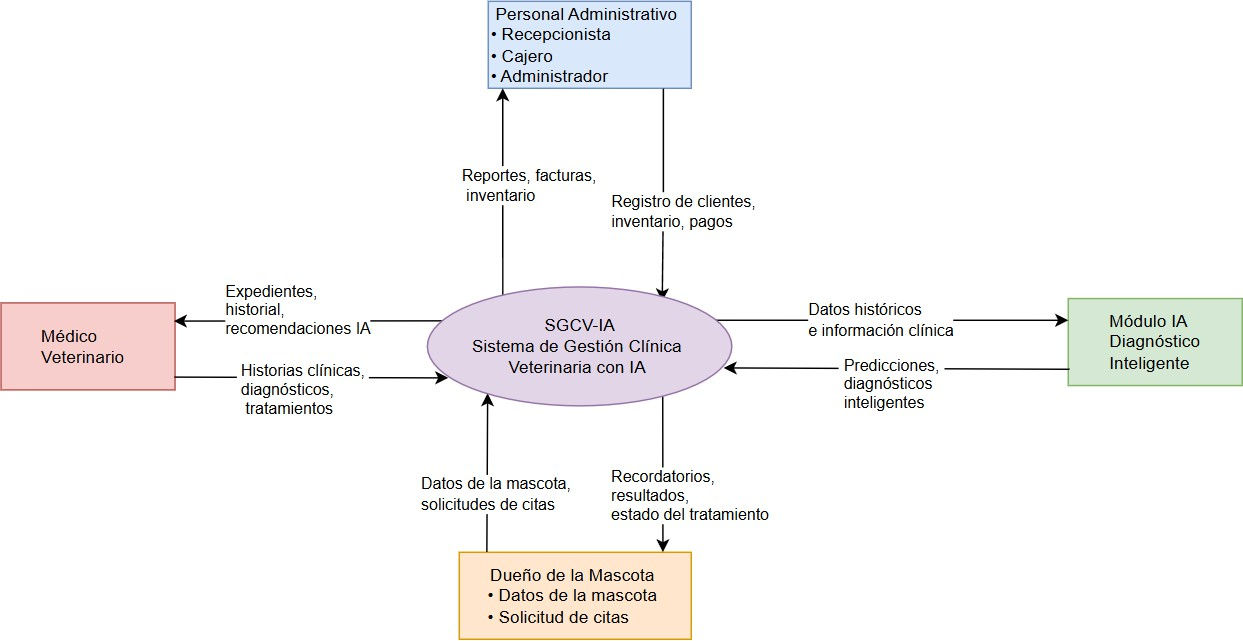
\includegraphics[width=6.2158in,height=3.205in]{./media/image1.jpeg}

\protect\phantomsection\label{_bookmark13}{}\emph{\textbf{Ilustración 1.
Diagrama de Contexto del Sistema}}

\subsubsection{Funciones del Producto}\label{funciones-del-producto}

\subsubsection{}\label{section}

\begin{quote}
A continuación, se presentan las principales funciones que ofrece el
SGCV-IA:
\end{quote}

{\def\LTcaptype{none} % do not increment counter
\begin{longtable}[]{@{}
  >{\centering\arraybackslash}p{(\linewidth - 4\tabcolsep) * \real{0.0530}}
  >{\raggedright\arraybackslash}p{(\linewidth - 4\tabcolsep) * \real{0.2151}}
  >{\raggedright\arraybackslash}p{(\linewidth - 4\tabcolsep) * \real{0.6880}}@{}}
\toprule\noalign{}
\begin{minipage}[b]{\linewidth}\centering
\textbf{N.°}
\end{minipage} & \begin{minipage}[b]{\linewidth}\raggedright
\begin{quote}
\textbf{Función principal}
\end{quote}
\end{minipage} & \begin{minipage}[b]{\linewidth}\centering
\textbf{Descripción}
\end{minipage} \\
\midrule\noalign{}
\endhead
\bottomrule\noalign{}
\endlastfoot
\textbf{F1} & \begin{minipage}[t]{\linewidth}\raggedright
\begin{quote}
Gestión de historiales clínicos
\end{quote}
\end{minipage} & \begin{minipage}[t]{\linewidth}\raggedright
\begin{quote}
Permite registrar, consultar y actualizar la información clínica de las
mascotas, incluyendo diagnósticos, tratamientos y antecedentes médicos.
\end{quote}
\end{minipage} \\
\textbf{F2} & \begin{minipage}[t]{\linewidth}\raggedright
\begin{quote}
Control de inventario
\end{quote}
\end{minipage} & \begin{minipage}[t]{\linewidth}\raggedright
\begin{quote}
Permite administrar el inventario de medicamentos e insumos, con alertas

de productos próximos a vencer o con bajo stock.
\end{quote}
\end{minipage} \\
\textbf{F3} & \begin{minipage}[t]{\linewidth}\raggedright
\begin{quote}
Asistente de diagnóstico con IA
\end{quote}
\end{minipage} & \begin{minipage}[t]{\linewidth}\raggedright
\begin{quote}
Analiza la información clínica del paciente para generar sugerencias
diagnósticas que sirvan de apoyo al médico veterinario.
\end{quote}
\end{minipage} \\
\textbf{F4} & \begin{minipage}[t]{\linewidth}\raggedright
\begin{quote}
Seguimiento

nutricional
\end{quote}
\end{minipage} & \begin{minipage}[t]{\linewidth}\raggedright
\begin{quote}
Registra el peso y otros datos del paciente para ofrecer recomendaciones

nutricionales de acuerdo con sus necesidades.
\end{quote}
\end{minipage} \\
\textbf{F5} & \begin{minipage}[t]{\linewidth}\raggedright
\begin{quote}
Gestión de citas
\end{quote}
\end{minipage} & \begin{minipage}[t]{\linewidth}\raggedright
\begin{quote}
Permite registrar, consultar, actualizar y organizar las citas de
atención de los pacientes.
\end{quote}
\end{minipage} \\
\textbf{F6} & \begin{minipage}[t]{\linewidth}\raggedright
\begin{quote}
Facturación
\end{quote}
\end{minipage} & \begin{minipage}[t]{\linewidth}\raggedright
\begin{quote}
Facilita el registro de los servicios prestados y la emisión de la
factura

correspondiente.
\end{quote}
\end{minipage} \\
\textbf{F7} & \begin{minipage}[t]{\linewidth}\raggedright
\begin{quote}
Generación de reportes
\end{quote}
\end{minipage} & \begin{minipage}[t]{\linewidth}\raggedright
\begin{quote}
Permite generar reportes relacionados con la atención clínica, el
inventario y la gestión de la clínica veterinaria.
\end{quote}
\end{minipage} \\
\textbf{F8} & \begin{minipage}[t]{\linewidth}\raggedright
\begin{quote}
Gestión de usuarios
\end{quote}
\end{minipage} & \begin{minipage}[t]{\linewidth}\raggedright
\begin{quote}
Administra las cuentas de los usuarios y los permisos de acceso según el

rol asignado dentro del sistema.
\end{quote}
\end{minipage} \\
\end{longtable}
}

\begin{quote}
\protect\phantomsection\label{_bookmark15}{}Tabla 4. Funciones del
Producto
\end{quote}

\subsubsection{Clases y características de
usuarios}\label{clases-y-caracteruxedsticas-de-usuarios}

\begin{quote}
Se identificaron los principales usuarios que interactuarán con el
SGCV-IA. Cada uno tendrá diferentes responsabilidades y niveles de
acceso según las actividades que realice dentro de la clínica
veterinaria.
\end{quote}

{\def\LTcaptype{none} % do not increment counter
\begin{longtable}[]{@{}
  >{\raggedright\arraybackslash}p{(\linewidth - 8\tabcolsep) * \real{0.1743}}
  >{\raggedright\arraybackslash}p{(\linewidth - 8\tabcolsep) * \real{0.1988}}
  >{\raggedright\arraybackslash}p{(\linewidth - 8\tabcolsep) * \real{0.3536}}
  >{\raggedright\arraybackslash}p{(\linewidth - 8\tabcolsep) * \real{0.0963}}
  >{\raggedright\arraybackslash}p{(\linewidth - 8\tabcolsep) * \real{0.1348}}@{}}
\toprule\noalign{}
\begin{minipage}[b]{\linewidth}\centering
\textbf{Tipo de usuario}
\end{minipage} & \begin{minipage}[b]{\linewidth}\raggedright
\begin{quote}
\textbf{Descripción}
\end{quote}
\end{minipage} & \begin{minipage}[b]{\linewidth}\raggedright
\begin{quote}
\textbf{Responsabilidades principales}
\end{quote}
\end{minipage} & \begin{minipage}[b]{\linewidth}\raggedright
\begin{quote}
\textbf{Nivel técnico}
\end{quote}
\end{minipage} & \begin{minipage}[b]{\linewidth}\raggedright
\begin{quote}
\textbf{Frecuencia de uso}
\end{quote}
\end{minipage} \\
\midrule\noalign{}
\endhead
\bottomrule\noalign{}
\endlastfoot
\textbf{Médico veterinario} &
\begin{minipage}[t]{\linewidth}\raggedright
\begin{quote}
Profesional encargado de la atención médica de las mascotas.
\end{quote}
\end{minipage} & \begin{minipage}[t]{\linewidth}\raggedright
\begin{quote}
Registrar y consultar historiales clínicos, emitir diagnósticos,
registrar tratamientos, realizar el seguimiento nutricional y utilizar
el asistente de Inteligencia Artificial

como apoyo en la toma de decisiones.
\end{quote}
\end{minipage} & \begin{minipage}[t]{\linewidth}\raggedright
\begin{quote}
Medio
\end{quote}
\end{minipage} & \begin{minipage}[t]{\linewidth}\raggedright
\begin{quote}
Diaria
\end{quote}
\end{minipage} \\
\textbf{Personal administrativo} &
\begin{minipage}[t]{\linewidth}\raggedright
\begin{quote}
Responsable de las actividades administrativas de la clínica.
\end{quote}
\end{minipage} & \begin{minipage}[t]{\linewidth}\raggedright
\begin{quote}
Gestionar citas, controlar el inventario de medicamentos e insumos,
registrar la facturación,

administrar la información de los pacientes y generar reportes.
\end{quote}
\end{minipage} & \begin{minipage}[t]{\linewidth}\raggedright
\begin{quote}
Básico

- Medio
\end{quote}
\end{minipage} & \begin{minipage}[t]{\linewidth}\raggedright
\begin{quote}
Diaria
\end{quote}
\end{minipage} \\
\textbf{Administrador} & \begin{minipage}[t]{\linewidth}\raggedright
\begin{quote}
Usuario encargado de la administración general del

sistema.
\end{quote}
\end{minipage} & \begin{minipage}[t]{\linewidth}\raggedright
\begin{quote}
Gestionar usuarios y permisos de acceso, supervisar el funcionamiento
del sistema y consultar los reportes generados.
\end{quote}
\end{minipage} & \begin{minipage}[t]{\linewidth}\raggedright
\begin{quote}
Medio
\end{quote}
\end{minipage} & \begin{minipage}[t]{\linewidth}\raggedright
\begin{quote}
Frecuente
\end{quote}
\end{minipage} \\
\end{longtable}
}

\begin{quote}
\protect\phantomsection\label{_bookmark17}{}\emph{\textbf{Tabla 5.
Clases y características de usuarios}}
\end{quote}

\paragraph{Características generales de los
usuarios}\label{caracteruxedsticas-generales-de-los-usuarios}

\subparagraph{Médico veterinario}\label{muxe9dico-veterinario}

\begin{itemize}
\item
  Posee conocimientos en medicina veterinaria.
\item
  Maneja herramientas informáticas a nivel básico o intermedio.
\item
  Utiliza el sistema durante la atención y seguimiento de los pacientes.
\end{itemize}

\subparagraph{Personal administrativo}\label{personal-administrativo}

\begin{itemize}
\item
  Cuenta con conocimientos básicos en el manejo de computadoras.
\item
  Utiliza el sistema para gestionar citas, inventario, facturación y
  consultas administrativas.
\item
  Hace uso del sistema de forma continua durante la jornada laboral.
\end{itemize}

\subparagraph{Administrador}\label{administrador}

\begin{itemize}
\item
  Tiene conocimientos básicos o intermedios del sistema.
\item
  Es responsable de administrar los usuarios y supervisar el
  funcionamiento general del SGCV-IA.
\item
  Accede al sistema de acuerdo con las necesidades de control y
  administración.
\end{itemize}

\subsubsection{Mapa de stakeholders}\label{mapa-de-stakeholders}

\begin{quote}
Para identificar el nivel de participación e influencia de los actores
involucrados en el desarrollo del SGCV-IA, se utilizó la matriz de
poder--interés de Mendelow. Esta herramienta permite definir la
estrategia de gestión más adecuada para cada stakeholder durante el
desarrollo e implementación del sistema.
\end{quote}

{\def\LTcaptype{none} % do not increment counter
\begin{longtable}[]{@{}
  >{\raggedright\arraybackslash}p{(\linewidth - 8\tabcolsep) * \real{0.2508}}
  >{\raggedright\arraybackslash}p{(\linewidth - 8\tabcolsep) * \real{0.0811}}
  >{\raggedright\arraybackslash}p{(\linewidth - 8\tabcolsep) * \real{0.0899}}
  >{\raggedright\arraybackslash}p{(\linewidth - 8\tabcolsep) * \real{0.1623}}
  >{\raggedright\arraybackslash}p{(\linewidth - 8\tabcolsep) * \real{0.3741}}@{}}
\toprule\noalign{}
\begin{minipage}[b]{\linewidth}\raggedright
\begin{quote}
\textbf{Stakeholder}
\end{quote}
\end{minipage} & \begin{minipage}[b]{\linewidth}\raggedright
\begin{quote}
\textbf{Poder}
\end{quote}
\end{minipage} & \begin{minipage}[b]{\linewidth}\raggedright
\textbf{Interés}
\end{minipage} & \begin{minipage}[b]{\linewidth}\raggedright
\begin{quote}
\textbf{Clasificación}
\end{quote}
\end{minipage} & \begin{minipage}[b]{\linewidth}\raggedright
\begin{quote}
\textbf{Estrategia de gestión}
\end{quote}
\end{minipage} \\
\midrule\noalign{}
\endhead
\bottomrule\noalign{}
\endlastfoot
\textbf{Propietario o administrador de la}

\textbf{clínica} & Alto & Alto & Gestionar de cerca &
\begin{minipage}[t]{\linewidth}\raggedright
\begin{quote}
Participar en la definición de requisitos, validar funcionalidades y

aprobar los avances del proyecto.
\end{quote}
\end{minipage} \\
\textbf{Médico veterinario} & Alto & Alto & Gestionar de cerca &
\begin{minipage}[t]{\linewidth}\raggedright
\begin{quote}
Validar los procesos clínicos, el

funcionamiento del asistente de IA y los historiales clínicos.
\end{quote}
\end{minipage} \\
\textbf{Personal administrativo} & Medio & Alto & Mantener informado &
\begin{minipage}[t]{\linewidth}\raggedright
\begin{quote}
Validar los procesos relacionados con citas, inventario, facturación y

reportes.
\end{quote}
\end{minipage} \\
\textbf{Equipo de desarrollo} & Alto & Alto & Gestionar de cerca &
\begin{minipage}[t]{\linewidth}\raggedright
\begin{quote}
Planificar, desarrollar, implementar y

verificar el cumplimiento de los requisitos del sistema.
\end{quote}
\end{minipage} \\
\textbf{Docente evaluador (Mg. Gleiston Guerrero Ulloa)} & Alto & Medio
& Mantener satisfecho & \begin{minipage}[t]{\linewidth}\raggedright
\begin{quote}
Supervisar el desarrollo del proyecto y verificar el cumplimiento de los
criterios académicos establecidos.
\end{quote}
\end{minipage} \\
\end{longtable}
}

\begin{quote}
\protect\phantomsection\label{_bookmark19}{}\emph{\textbf{Tabla 6. Mapa
Stakeholders del proyecto}}
\end{quote}

\subsubsection{Entorno operativo}\label{entorno-operativo}

\begin{quote}
l SGCV-IA será desarrollado como una aplicación web, compatible con los
principales navegadores, como \textbf{Google Chrome} (versión 100 o
superior) y \textbf{Mozilla Firefox} (versión 100 o superior). La
información del sistema se almacenará en una base de datos relacional
utilizando \textbf{MySQL}, lo que permitirá una administración segura y
organizada de los datos.
\end{quote}

\begin{itemize}
\item
  \textbf{Software:} El sistema funcionará en un servidor web y podrá
  ser utilizado desde computadoras de escritorio, portátiles y
  dispositivos móviles con acceso a un navegador web compatible.
\item
  \textbf{Conectividad:} Será necesario contar con conexión a Internet
  para acceder al sistema y utilizar todas sus funcionalidades,
  especialmente las relacionadas con el asistente de Inteligencia
  Artificial.
\item
  \textbf{Hardware:} El sistema podrá utilizarse desde computadoras de
  escritorio o portátiles para las actividades administrativas y desde
  dispositivos móviles para facilitar el acceso del médico
\end{itemize}

\begin{quote}
veterinario durante la atención de los pacientes. No requerirá equipos o
dispositivos especializados para su funcionamiento.
\end{quote}

\begin{itemize}
\item
  \textbf{Base de datos:} Toda la información clínica, administrativa y
  del inventario será almacenada en una base de datos \textbf{MySQL},
  garantizando la disponibilidad y organización de la información.
\end{itemize}

\subsubsection{Restricciones}\label{restricciones}

\begin{quote}
Las siguientes restricciones deberán considerarse durante el desarrollo
del SGCV-IA:
\end{quote}

\begin{itemize}
\item
  \textbf{Tecnológica:} el sistema deberá ser compatible con
  computadoras y dispositivos móviles mediante un navegador web.
\item
  \textbf{Conectividad:} será necesaria una conexión a Internet para
  utilizar todas las funcionalidades del sistema y el asistente de
  Inteligencia Artificial.
\item
  \textbf{Seguridad:} el acceso al sistema estará protegido mediante
  usuarios y permisos según el rol asignado.
\item
  \textbf{Usabilidad:} la interfaz deberá ser sencilla e intuitiva para
  facilitar su uso.
\item
  \textbf{Inteligencia Artificial:} las sugerencias generadas por la IA
  servirán únicamente como apoyo al médico veterinario y no reemplazarán
  su criterio profesional.
\end{itemize}

\subsubsection{Suposiciones y
Dependencias}\label{suposiciones-y-dependencias}

\paragraph{Suposiciones}\label{suposiciones}

\begin{quote}
Las siguientes suposiciones se consideran válidas durante el desarrollo
e implementación del sistema. Si cambian, los requisitos deberán
revisarse:
\end{quote}

\begin{itemize}
\item
  Se asume que los dueños de mascotas disponen de un número de teléfono
  celular activo registrado en la clínica, lo que permite el envío de
  recordatorios y resultados.
\item
  Se asume que la clínica cuenta con acceso a internet estable durante
  la mayor parte del horario de atención.
\item
  Se asume que el personal veterinario dispone de dispositivos móviles
  con sistemas operativos Android o iOS actualizados.
\item
  Se asume que el número de registros de pacientes se mantiene dentro de
  un rango manejable para la versión inicial del sistema.
\item
  Se asume la disponibilidad de datos históricos suficientes para
  alimentar y mejorar los modelos de inteligencia artificial.
\end{itemize}

\paragraph{Dependencias}\label{dependencias}

\begin{quote}
El sistema depende de los siguientes elementos externos:
\end{quote}

\begin{itemize}
\item
  Disponibilidad de conexión a internet para sincronización y acceso a
  la nube.
\item
  Disponibilidad de servicios de almacenamiento en la nube para datos
  clínicos.
\item
  Acceso a la API de WhatsApp Business o servicio equivalente para el
  envío de notificaciones.
\item
  Disponibilidad de un proveedor externo de modelos de IA (LLM) para
  funcionalidades inteligentes.
\item
  Infraestructura mínima de dispositivos móviles y/o computadoras en la
  clínica
\end{itemize}

\section{Requisitos Específicos}\label{requisitos-especuxedficos}

\subsubsection{Interfaces externas}\label{interfaces-externas}

\paragraph{Interfaz de usuario}\label{interfaz-de-usuario}

\begin{quote}
A continuación se describen las pantallas principales de la interfaz de
usuario de SGCV-IA, identificadas a partir de las funciones del producto
definidas en la Sección 2.2 y de los hallazgos de las entrevistas de
elicitación (Apéndice B). Cada pantalla se vincula con la función o
módulo que soporta; la referencia a los requisitos funcionales formales
(RF-XX) se completará en la Sección 3.2 una vez consolidada su
numeración definitiva.
\end{quote}

{\def\LTcaptype{none} % do not increment counter
\begin{longtable}[]{@{}
  >{\raggedright\arraybackslash}p{(\linewidth - 4\tabcolsep) * \real{0.2458}}
  >{\raggedright\arraybackslash}p{(\linewidth - 4\tabcolsep) * \real{0.5532}}
  >{\raggedright\arraybackslash}p{(\linewidth - 4\tabcolsep) * \real{0.1843}}@{}}
\toprule\noalign{}
\begin{minipage}[b]{\linewidth}\raggedright
\textbf{Pantalla}
\end{minipage} & \begin{minipage}[b]{\linewidth}\raggedright
\begin{quote}
\textbf{Descripción}
\end{quote}
\end{minipage} & \begin{minipage}[b]{\linewidth}\raggedright
\textbf{Función relacionada (Sec. 2.2)}
\end{minipage} \\
\midrule\noalign{}
\endhead
\bottomrule\noalign{}
\endlastfoot
\textbf{Login / Selección de rol} &
\begin{minipage}[t]{\linewidth}\raggedright
\begin{quote}
Autenticación con usuario y contraseña; redirección al panel
correspondiente según el rol asignado (RBAC):

Médico Veterinario o Personal Administrativo.
\end{quote}
\end{minipage} & F9 \\
\textbf{Dashboard general} & \begin{minipage}[t]{\linewidth}\raggedright
\begin{quote}
Resumen del día: citas próximas, alertas de inventario por

vencer o agotarse, pacientes con seguimiento pendiente y accesos rápidos
según el rol del usuario.
\end{quote}
\end{minipage} & F1, F2, F5 \\
\textbf{Gestión de Historiales Clínicos} &
\begin{minipage}[t]{\linewidth}\raggedright
\begin{quote}
Listado de pacientes con búsqueda por nombre del animal o del dueño;
ficha de detalle con datos generales, historial

de consultas, diagnósticos y tratamientos previos.
\end{quote}
\end{minipage} & F1 \\
\textbf{Registro de Consulta} &
\begin{minipage}[t]{\linewidth}\raggedright
\begin{quote}
Formulario de nueva consulta (motivo, síntomas,

diagnóstico, tratamiento, dosis y frecuencia), con acceso directo al
panel de sugerencias de IA durante el registro.
\end{quote}
\end{minipage} & F1, F3 \\
\textbf{Panel de Diagnóstico Asistido por IA} &
\begin{minipage}[t]{\linewidth}\raggedright
\begin{quote}
Vista de los diagnósticos diferenciales sugeridos por el módulo de IA
junto con su respaldo bibliográfico; el veterinario puede aceptar,
modificar o rechazar cada

sugerencia antes de registrarla.
\end{quote}
\end{minipage} & F3 \\
\textbf{Seguimiento Nutricional} &
\begin{minipage}[t]{\linewidth}\raggedright
\begin{quote}
Registro cronológico de peso y condición corporal del

paciente, con gráfico de tendencia y recomendaciones de alimentación
generadas según raza, edad y peso.
\end{quote}
\end{minipage} & F4 \\
\textbf{Gestión de Citas y Recordatorios} &
\begin{minipage}[t]{\linewidth}\raggedright
\begin{quote}
Calendario de citas programadas por paciente, registro de
asistencia/inasistencia y configuración de recordatorios

automáticos enviados al dueño.
\end{quote}
\end{minipage} & F5 \\
\textbf{Comunicación con Dueños} &
\begin{minipage}[t]{\linewidth}\raggedright
\begin{quote}
Historial de comunicaciones (llamadas, WhatsApp) por

paciente, con opción de adjuntar y enviar resultados de exámenes
directamente desde la plataforma.
\end{quote}
\end{minipage} & F6 \\
\textbf{Facturación y Cobro} &
\begin{minipage}[t]{\linewidth}\raggedright
\begin{quote}
Formulario de cobro post-consulta en un máximo de tres pasos: selección
de servicios y productos utilizados, cálculo del monto total y emisión
del comprobante.
\end{quote}
\end{minipage} & F7 \\
\textbf{Inventario de Bodega} &
\begin{minipage}[t]{\linewidth}\raggedright
\begin{quote}
Listado de insumos y medicamentos con stock actual y fecha de
vencimiento; formulario de entradas/salidas y

panel de alertas de vencimiento próximo o stock mínimo.
\end{quote}
\end{minipage} & F2 \\
\textbf{Reportes y Exportación} &
\begin{minipage}[t]{\linewidth}\raggedright
\begin{quote}
Generación de reportes del historial clínico y de indicadores operativos
(consultas, facturación, inventario),

exportables en formato PDF para referencias a otras clínicas.
\end{quote}
\end{minipage} & F8 \\
\end{longtable}
}

{\def\LTcaptype{none} % do not increment counter
\begin{longtable}[]{@{}
  >{\raggedright\arraybackslash}p{(\linewidth - 4\tabcolsep) * \real{0.2458}}
  >{\raggedright\arraybackslash}p{(\linewidth - 4\tabcolsep) * \real{0.5532}}
  >{\raggedright\arraybackslash}p{(\linewidth - 4\tabcolsep) * \real{0.1843}}@{}}
\toprule\noalign{}
\begin{minipage}[b]{\linewidth}\raggedright
\textbf{Gestión de Usuarios y Accesos}
\end{minipage} & \begin{minipage}[b]{\linewidth}\raggedright
\begin{quote}
Alta y edición de cuentas de personal, asignación de rol

(Médico Veterinario / Personal Administrativo) y permisos de acceso a
cada módulo.
\end{quote}
\end{minipage} & \begin{minipage}[b]{\linewidth}\raggedright
F9
\end{minipage} \\
\midrule\noalign{}
\endhead
\bottomrule\noalign{}
\endlastfoot
\end{longtable}
}

\protect\phantomsection\label{_bookmark24}{}\emph{\textbf{Tabla 7.
Interfaz de usuario}}

\begin{quote}
Los mockups de alta fidelidad correspondientes a cada pantalla fueron
desarrollados en Figma y se presentan a continuación como capturas del
prototipo; los archivos editables se incluyen en la carpeta
modelos/mockups/ del repositorio GitHub del proyecto, conforme a lo
establecido en la guía de entrega.
\end{quote}

\subparagraph{Mockups de interfaz (capturas del
prototipo)}\label{mockups-de-interfaz-capturas-del-prototipo}

\begin{quote}
A continuación se presentan las capturas del prototipo de alta fidelidad
correspondientes a cada pantalla descrita en la Tabla de la sección
3.1.1, desarrolladas como parte del diseño de interfaz del sistema
SGCV-IA.
\end{quote}

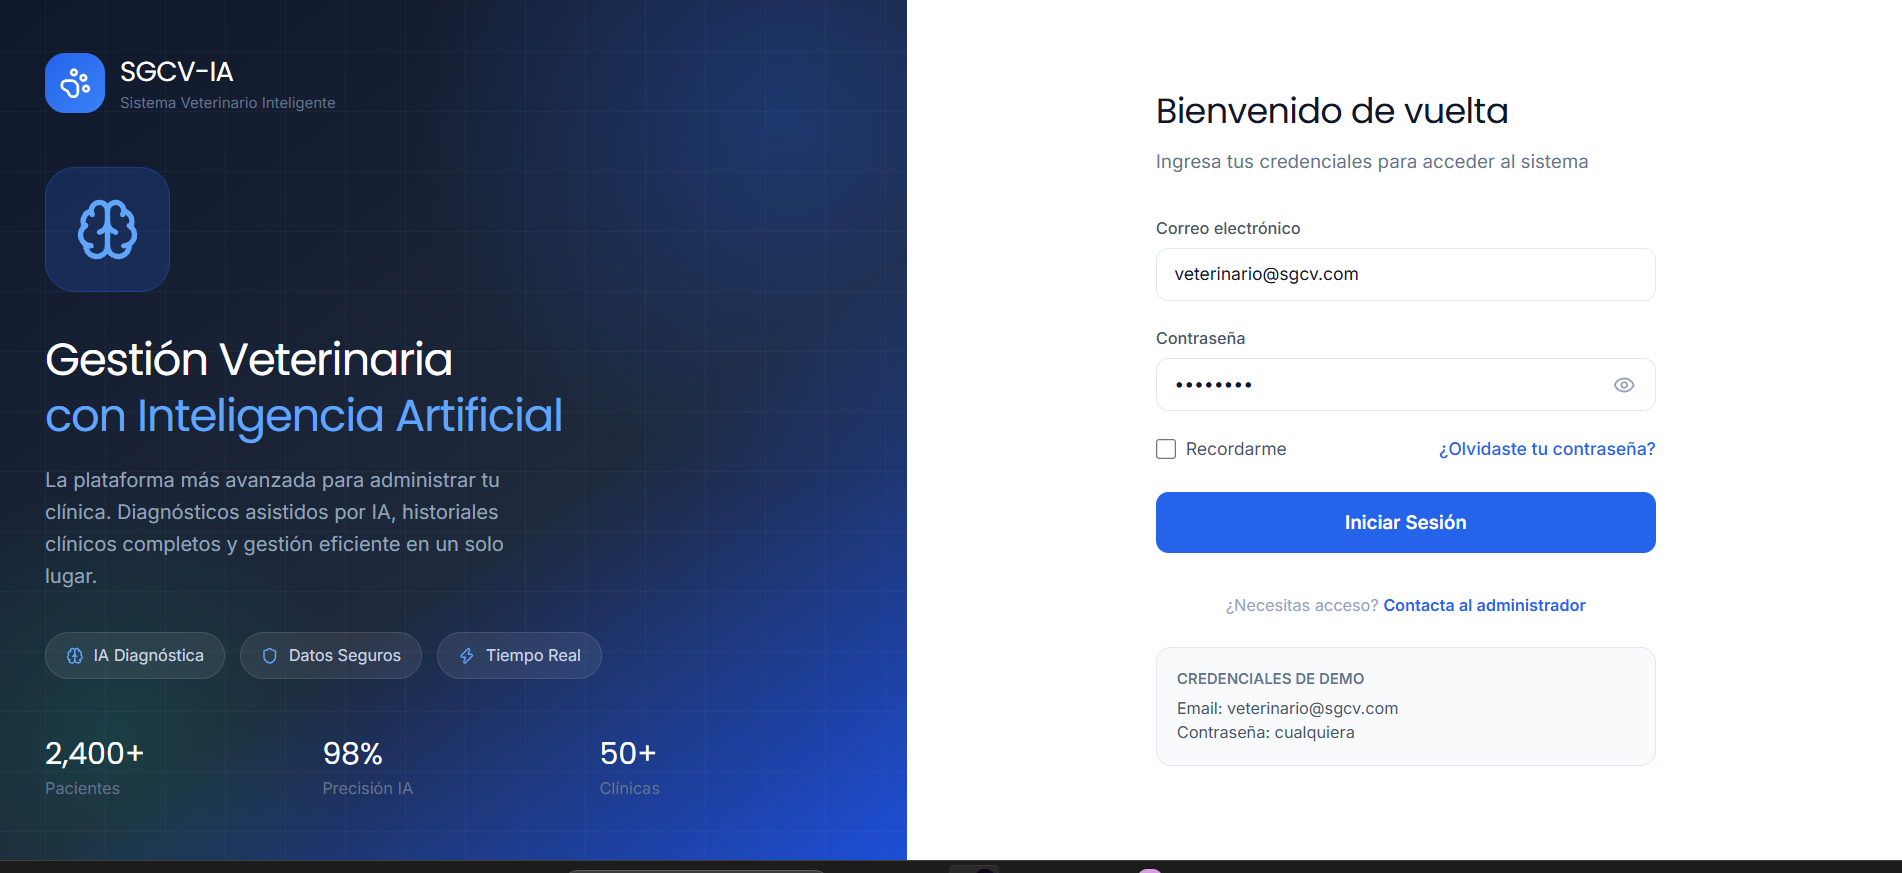
\includegraphics[width=6.79514in,height=3.11875in]{./media/image2.png}

\protect\phantomsection\label{_bookmark25}{}Ilustración 2. Login /
Selección de rol

\begin{quote}
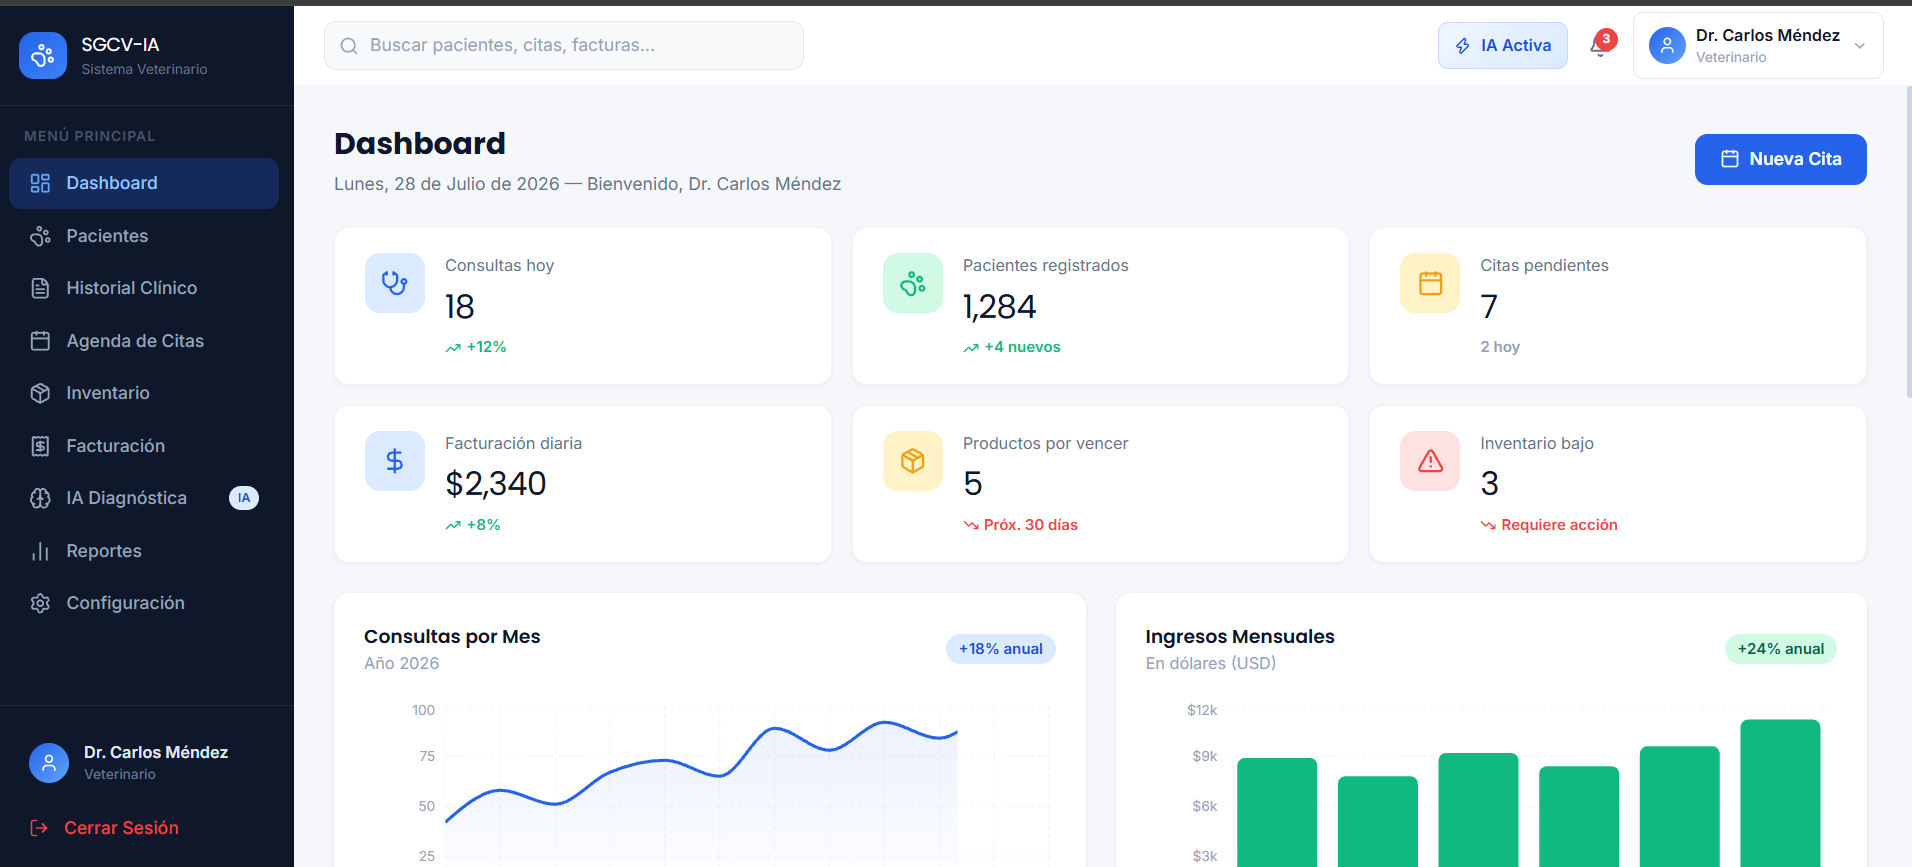
\includegraphics[width=6.79514in,height=3.08125in]{./media/image3.png}
\end{quote}

\protect\phantomsection\label{_bookmark26}{}Ilustración 3. Dashboard
general

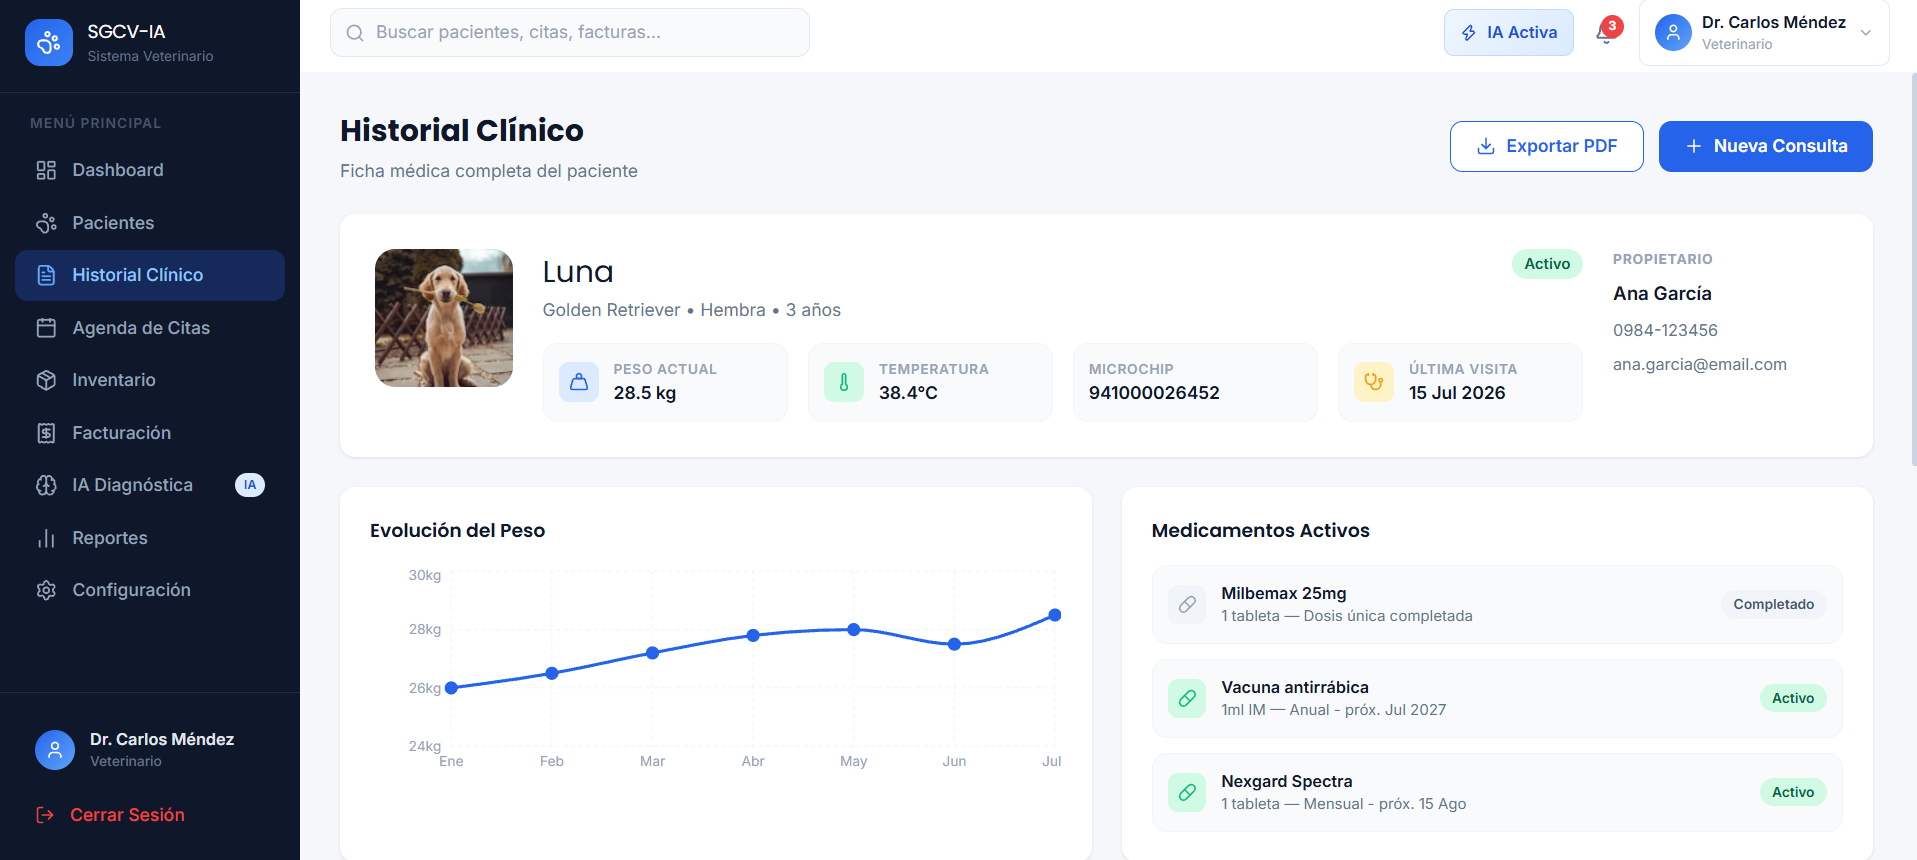
\includegraphics[width=6.79514in,height=3.04861in]{./media/image4.png}

\protect\phantomsection\label{_bookmark27}{}Ilustración 4. Gestión de
Historiales Clínicos

\begin{quote}
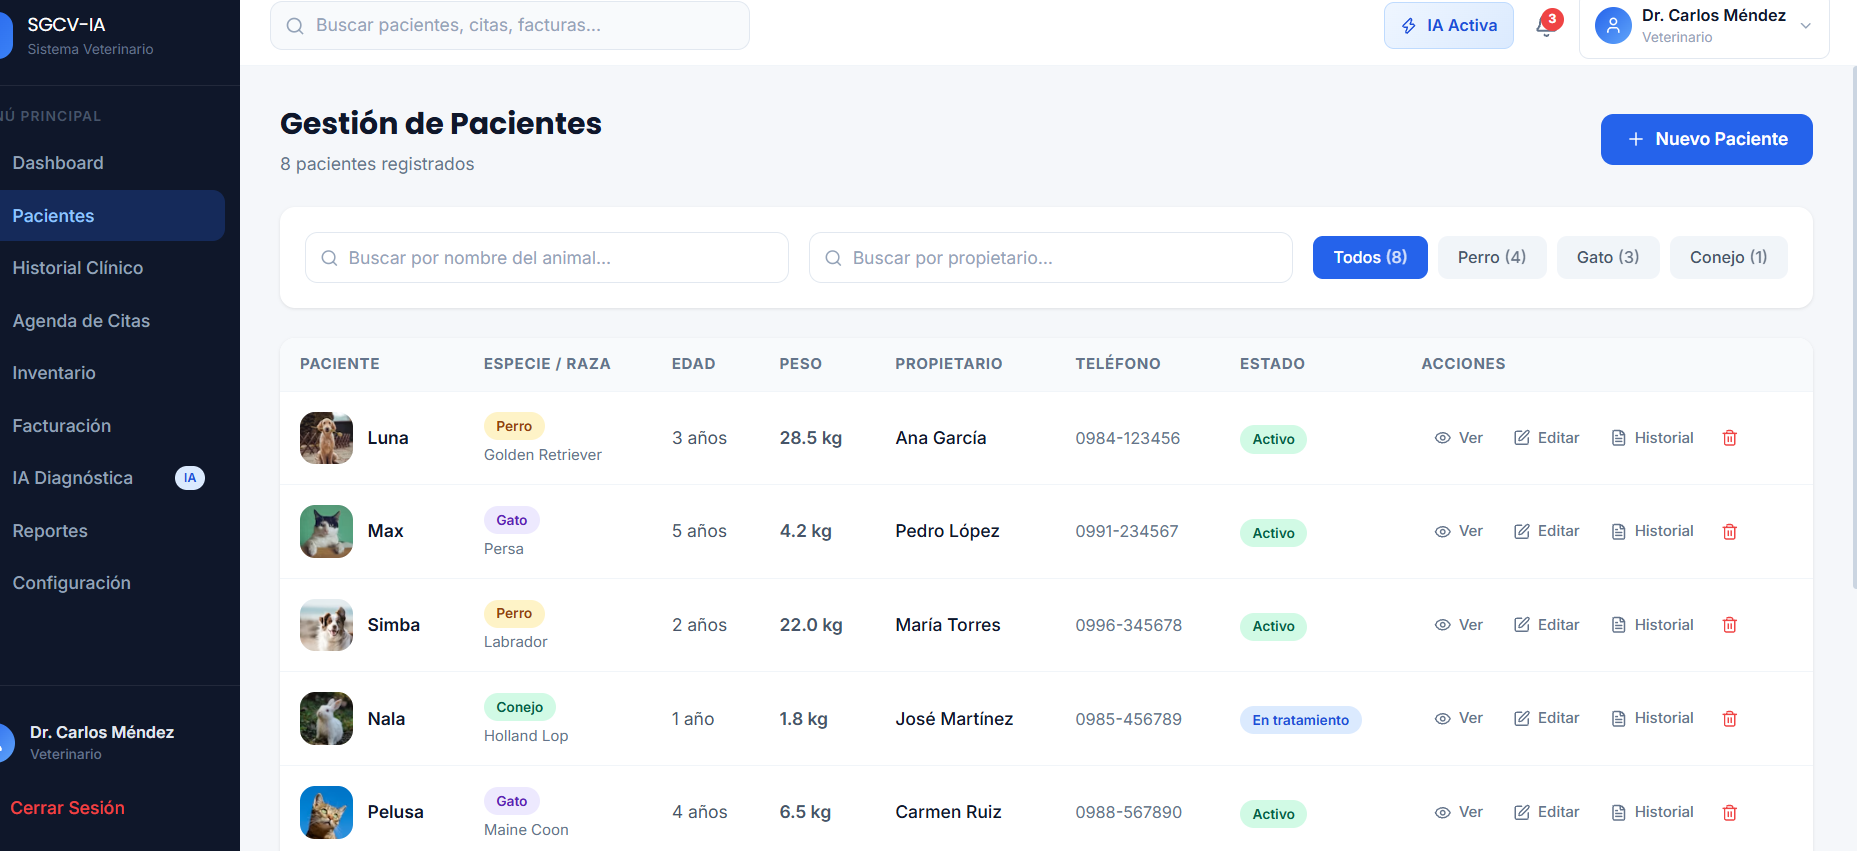
\includegraphics[width=6.79514in,height=3.11389in]{./media/image5.png}

\protect\phantomsection\label{_bookmark28}{}Ilustración 5. Registro de
pasientes
\end{quote}

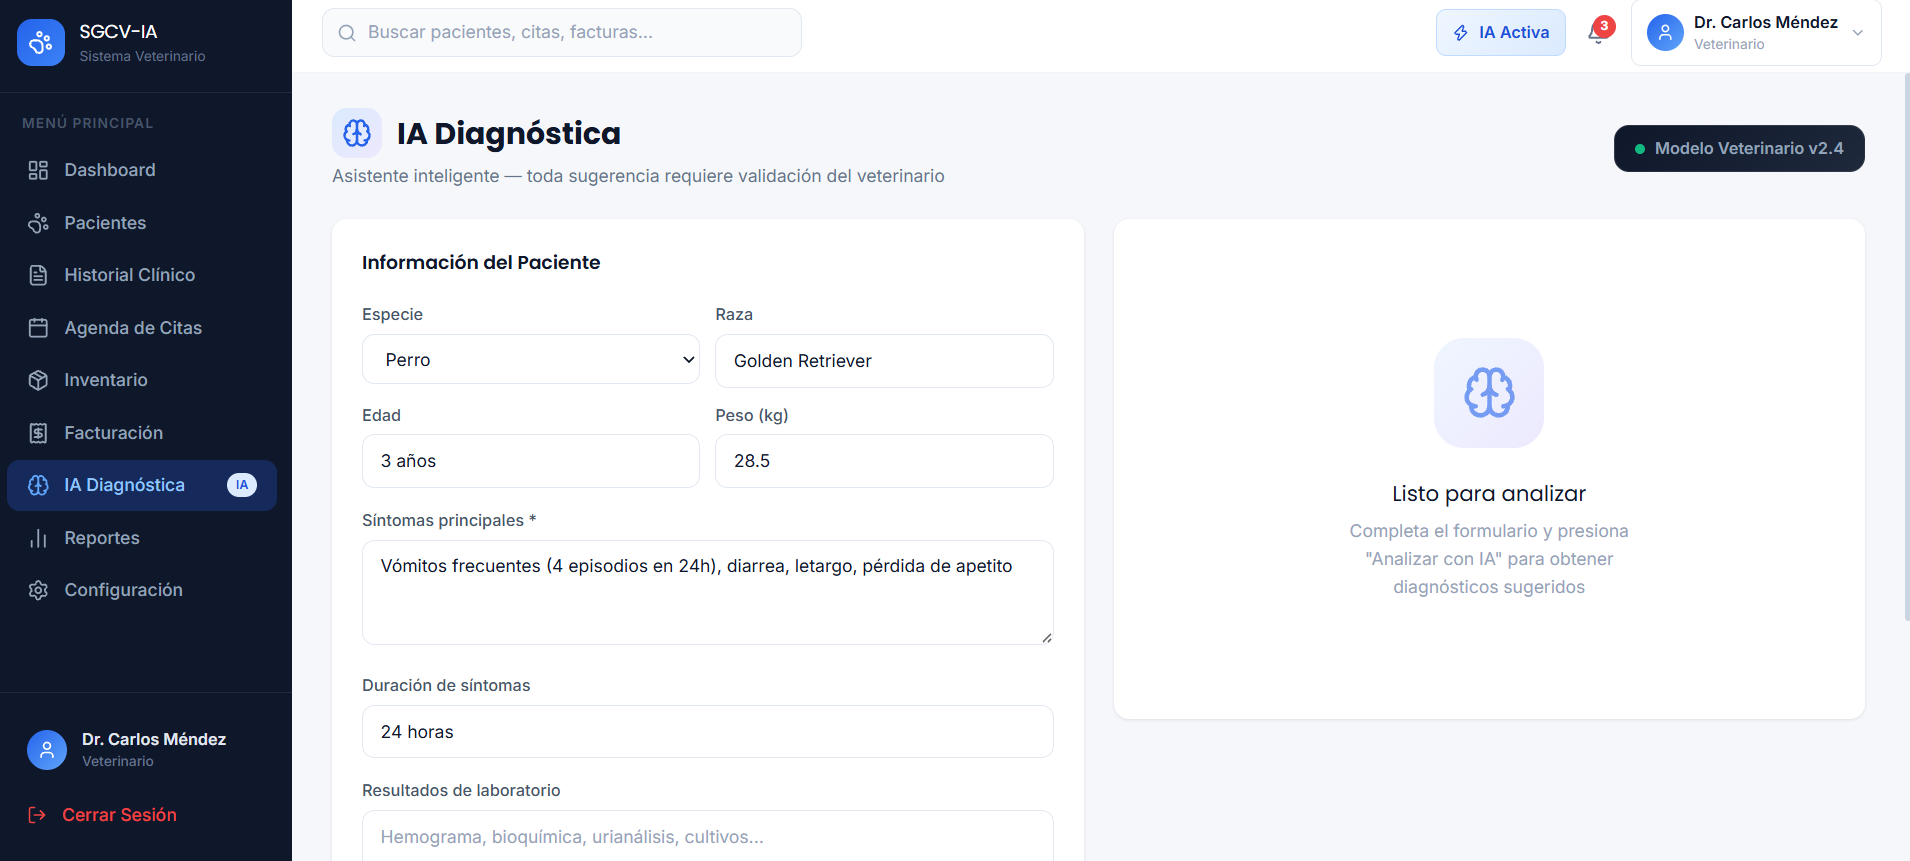
\includegraphics[width=6.79514in,height=3.06319in]{./media/image6.png}

\protect\phantomsection\label{_bookmark29}{}Ilustración 6. Panel de
Diagnóstico Asistido por IA

\begin{quote}
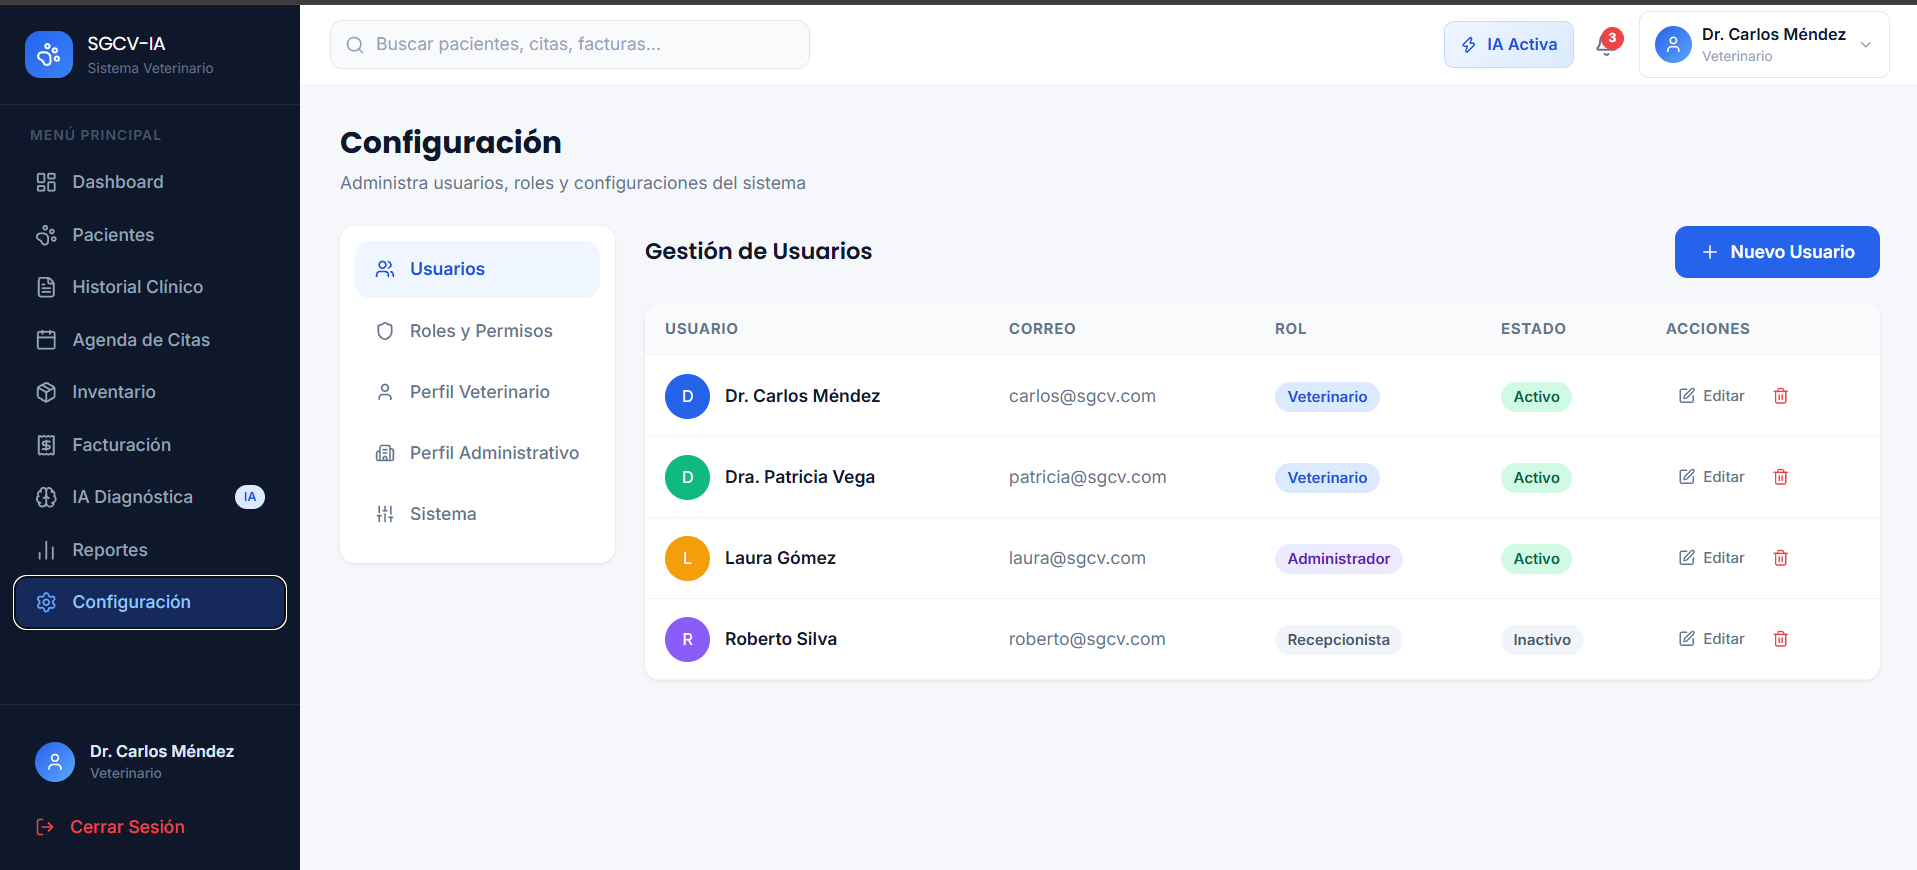
\includegraphics[width=6.79514in,height=3.08403in]{./media/image7.png}
\end{quote}

\protect\phantomsection\label{_bookmark30}{}Ilustración 7. Configuraion

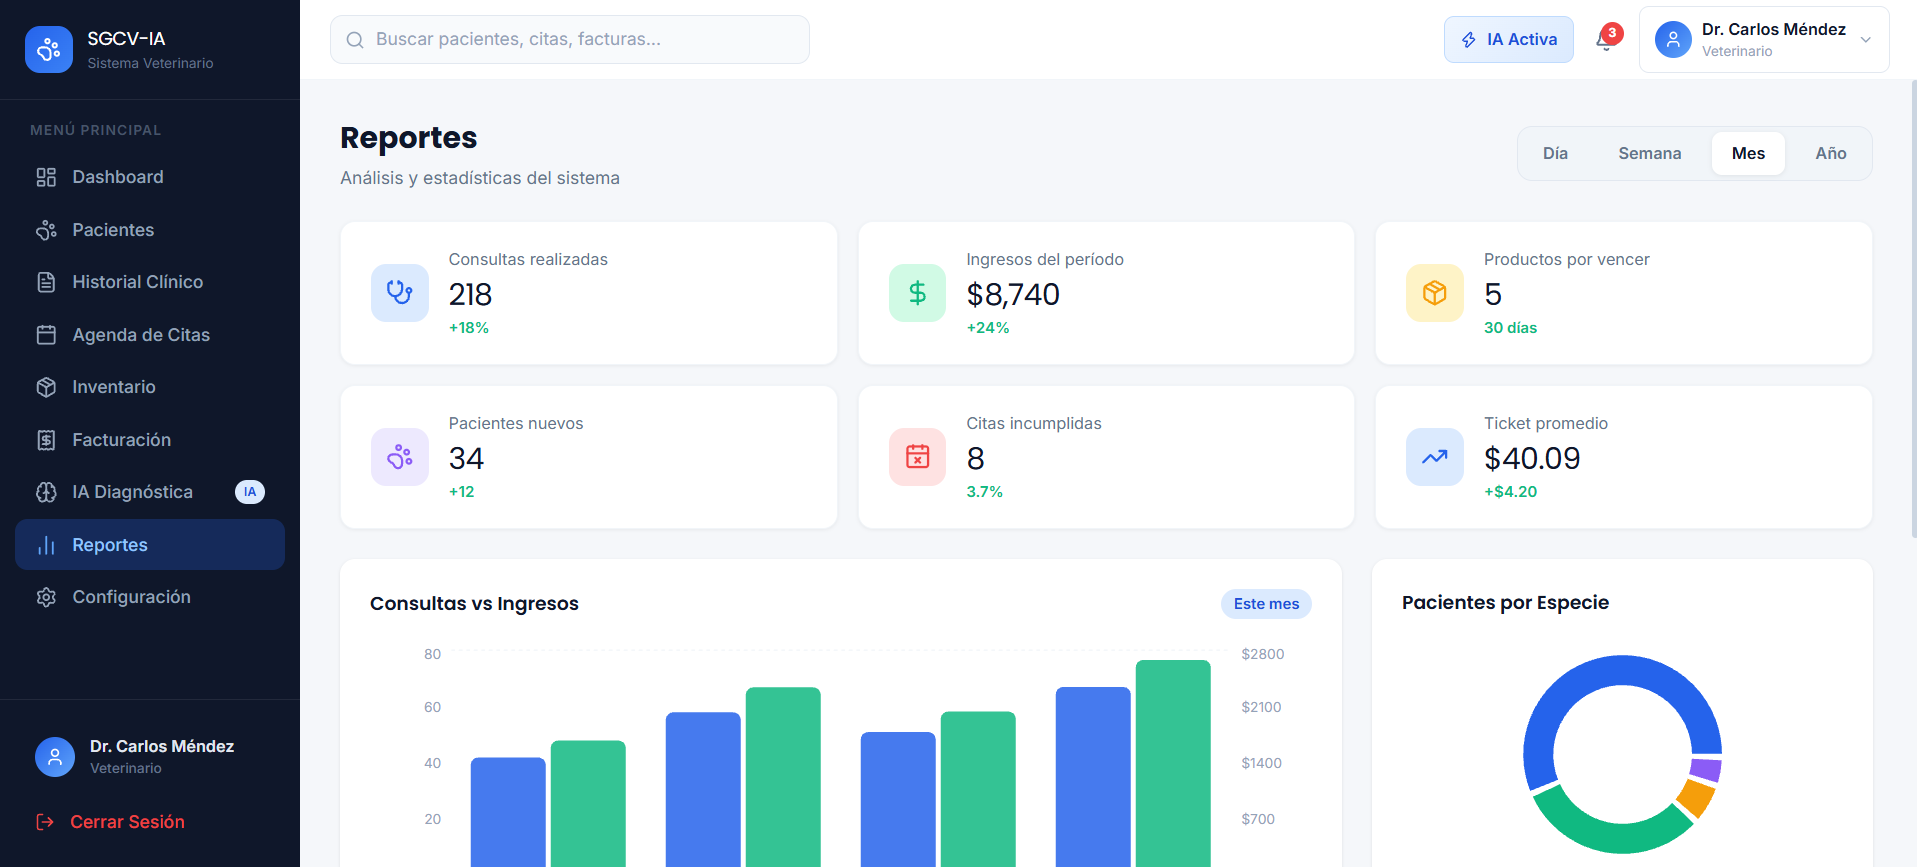
\includegraphics[width=6.79514in,height=3.07292in]{./media/image8.png}

\protect\phantomsection\label{_bookmark31}{}Ilustración 8 Gestión de
Citas y Recordatorios

\begin{quote}
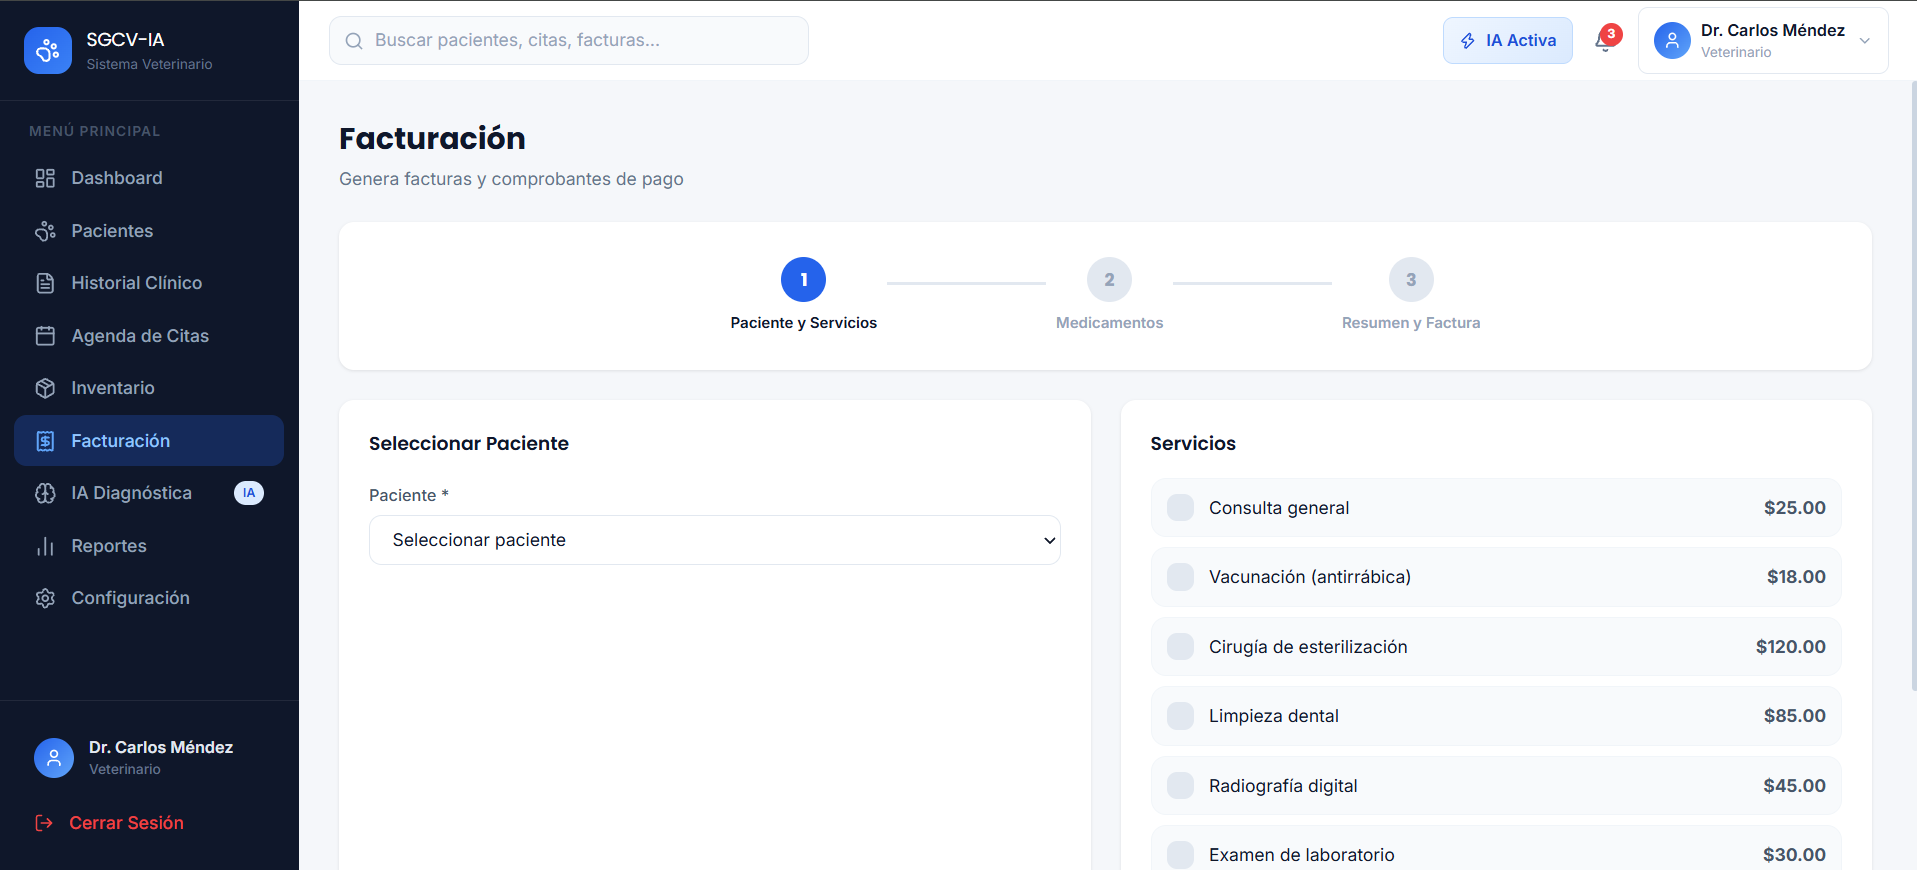
\includegraphics[width=6.79514in,height=3.08403in]{./media/image9.png}
\end{quote}

\protect\phantomsection\label{_bookmark32}{}Ilustración 9. Comunicación
con Dueños

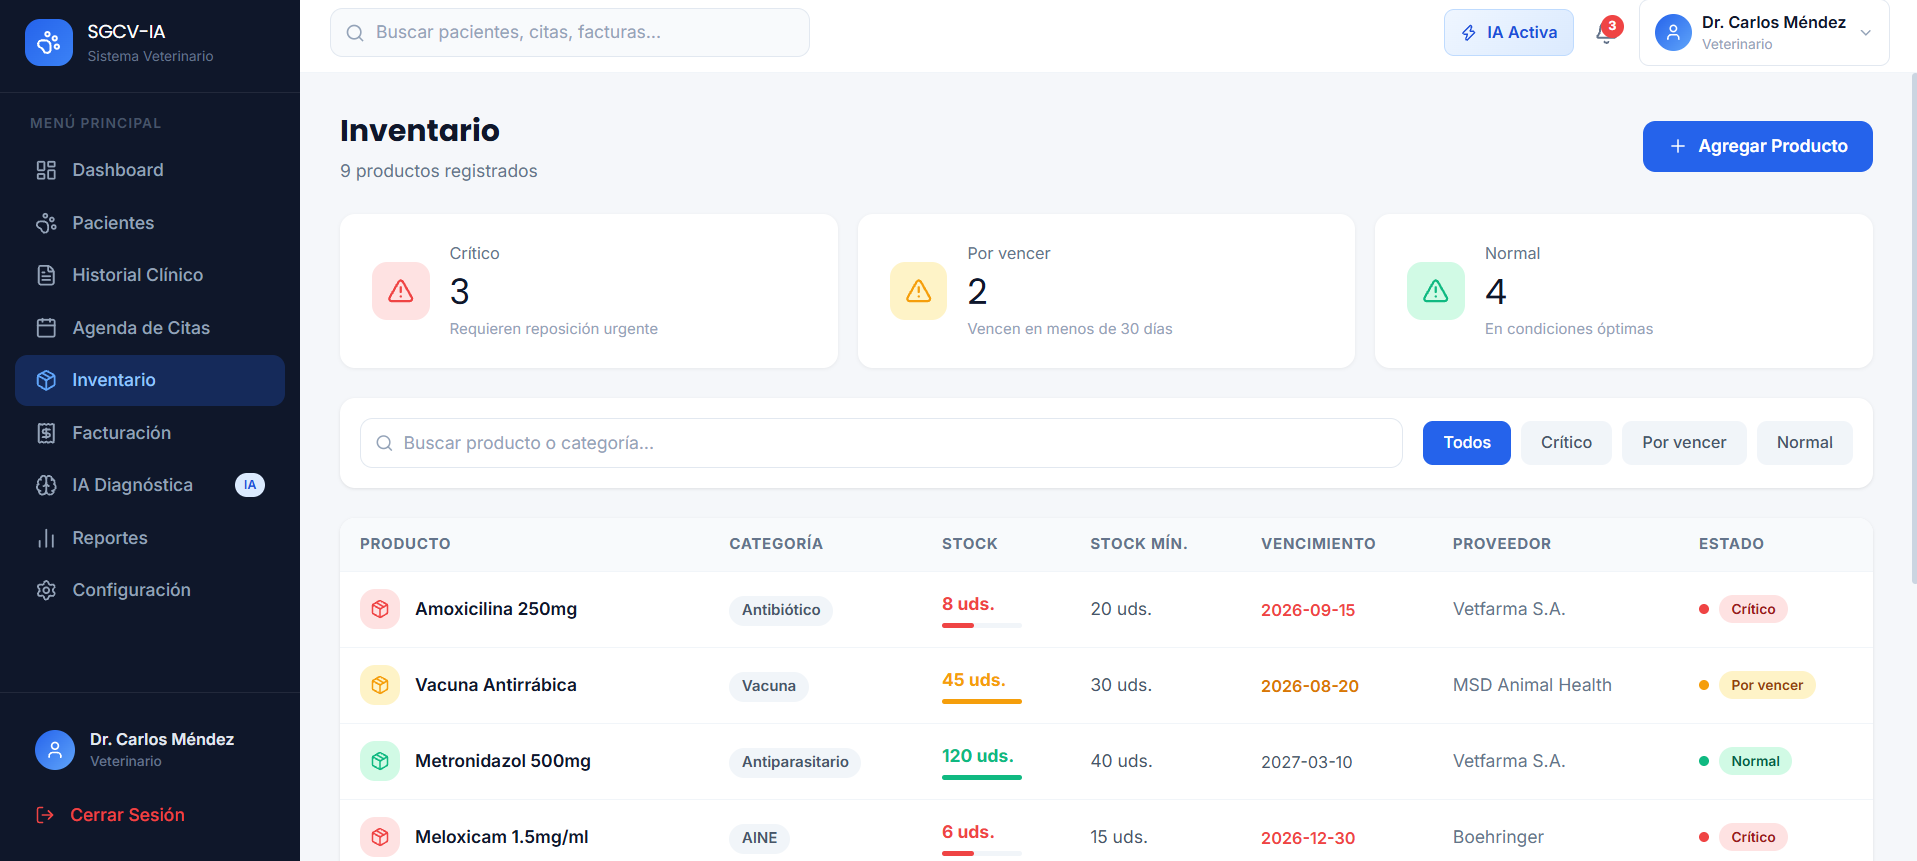
\includegraphics[width=6.79514in,height=3.05208in]{./media/image10.png}

\protect\phantomsection\label{_bookmark33}{}Ilustración 10. Inventario
de Bodega

\protect\phantomsection\label{_bookmark35}{}

\subparagraph{Prototipo interactivo en
Figma}\label{prototipo-interactivo-en-figma}

\begin{quote}
El prototipo navegable de alta fidelidad, con todas las pantallas
listadas anteriormente, puede consultarse en el siguiente enlace de
Figma:

\href{https://www.figma.com/make/gYiCFRRe7MInCu8yvNY2Bh/Veterinary-Clinic-Management-App?t=ZG1PmrVgNV05SnQY-1}{\ul{https://www.figma.com/make/gYiCFRRe7MInCu8yvNY2Bh/Veterinary-Clinic-Management-App}}
\end{quote}

\paragraph{Interfaz de hardware}\label{interfaz-de-hardware}

\begin{quote}
SGCV-IA es un sistema de gestión clínica veterinaria desarrollado como
aplicación de escritorio (Windows Forms / C\#); por ello, su interfaz de
hardware se limita a los dispositivos físicos sobre los cuales se
ejecuta y con los que interactúa el personal de la clínica durante la
consulta, la facturación y la gestión de inventario. La referencia a las
funciones del producto (Sec. 2.2) se mantiene a modo orientativo, en
espera de su vinculación definitiva con los requisitos funcionales
formales (RF-XX) en la Sección 3.2.
\end{quote}

{\def\LTcaptype{none} % do not increment counter
\begin{longtable}[]{@{}
  >{\raggedright\arraybackslash}p{(\linewidth - 4\tabcolsep) * \real{0.2458}}
  >{\raggedright\arraybackslash}p{(\linewidth - 4\tabcolsep) * \real{0.5532}}
  >{\raggedright\arraybackslash}p{(\linewidth - 4\tabcolsep) * \real{0.1843}}@{}}
\toprule\noalign{}
\begin{minipage}[b]{\linewidth}\raggedright
\textbf{Componente}
\end{minipage} & \begin{minipage}[b]{\linewidth}\raggedright
\begin{quote}
\textbf{Descripción}
\end{quote}
\end{minipage} & \begin{minipage}[b]{\linewidth}\raggedright
\textbf{Función relacionada (Sec.}

\textbf{2.2)}
\end{minipage} \\
\midrule\noalign{}
\endhead
\bottomrule\noalign{}
\endlastfoot
\textbf{Equipos de cómputo cliente} &
\begin{minipage}[t]{\linewidth}\raggedright
\begin{quote}
Computadoras de escritorio o portátiles con sistema operativo Windows 10
o superior, ubicadas en recepción, consultorio y administración.
Resolución mínima de pantalla de 1366x768 píxeles, mínimo 4 GB de RAM y
conexión a la

red local (LAN) de la clínica.
\end{quote}
\end{minipage} & F1--F9 \\
\textbf{Periféricos de entrada} &
\begin{minipage}[t]{\linewidth}\raggedright
\begin{quote}
Teclado y mouse estándar para el ingreso de datos en los formularios de
historiales clínicos, consultas, facturación e inventario. No se
requiere hardware especializado adicional

en el alcance actual del sistema.
\end{quote}
\end{minipage} & F1, F3, F7 \\
\textbf{Periféricos de salida} &
\begin{minipage}[t]{\linewidth}\raggedright
\begin{quote}
Impresora local o de red (matricial o láser) conectada al equipo de
recepción/administración, utilizada para la emisión de comprobantes de
cobro y la impresión de reportes

exportados en formato PDF.
\end{quote}
\end{minipage} & F7, F8 \\
\textbf{Almacenamiento y conectividad} &
\begin{minipage}[t]{\linewidth}\raggedright
\begin{quote}
Conexión permanente, mediante red local cableada o inalámbrica, al
servidor donde reside la base de datos del sistema. No se contempla
almacenamiento local independiente en los equipos cliente más allá de la
caché

temporal propia de la aplicación.
\end{quote}
\end{minipage} & F1--F9 \\
\end{longtable}
}

\protect\phantomsection\label{_bookmark36}{}\emph{\textbf{Tabla 8.
Interfaz de hardware}}

\begin{quote}
El sistema no requiere hardware especializado adicional (lectores
biométricos, sensores u otros dispositivos IoT) en su alcance actual;
cualquier ampliación futura del hardware de soporte se documentará en
versiones posteriores del ERS.
\end{quote}

\paragraph{Interfaz de software}\label{interfaz-de-software}

\begin{quote}
A continuación, se describen los componentes de software, formatos de
intercambio e integraciones con los que interactúa SGCV-IA como
aplicación de escritorio (Windows Forms / C\#). La referencia a las
funciones del producto (Sec. 2.2) se mantiene a modo orientativo, en
espera de su vinculación definitiva con los requisitos funcionales
formales (RF-XX) en la Sección 3.2.
\end{quote}

{\def\LTcaptype{none} % do not increment counter
\begin{longtable}[]{@{}
  >{\raggedright\arraybackslash}p{(\linewidth - 4\tabcolsep) * \real{0.2458}}
  >{\raggedright\arraybackslash}p{(\linewidth - 4\tabcolsep) * \real{0.5532}}
  >{\raggedright\arraybackslash}p{(\linewidth - 4\tabcolsep) * \real{0.1843}}@{}}
\toprule\noalign{}
\begin{minipage}[b]{\linewidth}\raggedright
\textbf{Componente}
\end{minipage} & \begin{minipage}[b]{\linewidth}\raggedright
\begin{quote}
\textbf{Descripción}
\end{quote}
\end{minipage} & \begin{minipage}[b]{\linewidth}\raggedright
\textbf{Función relacionada (Sec. 2.2)}
\end{minipage} \\
\midrule\noalign{}
\endhead
\bottomrule\noalign{}
\endlastfoot
\textbf{Sistema operativo y plataforma} &
\begin{minipage}[t]{\linewidth}\raggedright
\begin{quote}
Aplicación de escritorio desarrollada en C\# sobre el framework

.NET (Windows Forms), compatible con Windows 10 o superior. No requiere
instalación de máquina virtual ni dependencias de plataformas externas
para su ejecución en el cliente.
\end{quote}
\end{minipage} & F1--F9 \\
\textbf{Base de datos} & \begin{minipage}[t]{\linewidth}\raggedright
\begin{quote}
Motor de base de datos relacional (SQL Server o equivalente) alojado en
el servidor de la clínica, accedido mediante ADO.NET o un ORM (p. ej.
Entity Framework) a través de la red local. Almacena historiales
clínicos, citas, inventario,

facturación y usuarios.
\end{quote}
\end{minipage} & F1, F2, F5, F7, F9 \\
\textbf{Formato de intercambio de datos} &
\begin{minipage}[t]{\linewidth}\raggedright
\begin{quote}
Generación de reportes exportables en formato PDF (historial clínico,
indicadores operativos) mediante una biblioteca de generación de
documentos integrada en la aplicación.

Intercambio interno de datos en formato estructurado (objetos

.NET / DataSet) entre los módulos del sistema.
\end{quote}
\end{minipage} & F8 \\
\textbf{Módulo de IA} & \begin{minipage}[t]{\linewidth}\raggedright
\begin{quote}
Comunicación con el módulo de diagnóstico asistido mediante una API
interna (REST/HTTP) que recibe los datos de la consulta (síntomas,
motivo) y devuelve los diagnósticos diferenciales sugeridos junto con su
respaldo bibliográfico.
\end{quote}
\end{minipage} & F3 \\
\textbf{Comunicación con terceros} &
\begin{minipage}[t]{\linewidth}\raggedright
\begin{quote}
Integración con servicios externos de mensajería (p. ej. WhatsApp
Business API) y/o correo electrónico para el envío de
\end{quote}
\end{minipage} & F5, F6 \\
\end{longtable}
}

{\def\LTcaptype{none} % do not increment counter
\begin{longtable}[]{@{}
  >{\raggedright\arraybackslash}p{(\linewidth - 4\tabcolsep) * \real{0.2458}}
  >{\raggedright\arraybackslash}p{(\linewidth - 4\tabcolsep) * \real{0.5532}}
  >{\raggedright\arraybackslash}p{(\linewidth - 4\tabcolsep) * \real{0.1843}}@{}}
\toprule\noalign{}
\begin{minipage}[b]{\linewidth}\raggedright
\end{minipage} & \begin{minipage}[b]{\linewidth}\raggedright
\begin{quote}
recordatorios de citas y resultados de exámenes a los dueños de las
mascotas.
\end{quote}
\end{minipage} & \begin{minipage}[b]{\linewidth}\raggedright
\end{minipage} \\
\midrule\noalign{}
\endhead
\bottomrule\noalign{}
\endlastfoot
\end{longtable}
}

\subparagraph{Tabla 9. Interfaz de
software}\label{tabla-9.-interfaz-de-software}

\begin{quote}
El módulo de IA y las integraciones de comunicación con terceros se
diseñarán como componentes desacoplados del núcleo transaccional del
sistema, de forma que su eventual indisponibilidad no comprometa el
funcionamiento de los módulos clínicos y administrativos principales.
\end{quote}

\paragraph{Interfaces de
comunicación}\label{interfaces-de-comunicaciuxf3n}

\begin{quote}
\emph{Sección pendiente de elaboración.}
\end{quote}

\subsubsection{Requisitos Funcionales}\label{requisitos-funcionales}

\begin{quote}
A continuación, se formalizan los requisitos funcionales (RF) de
SGCV-IA, derivados de los requisitos crudos (RC) identificados durante
la elicitación (Sección III del documento de Entrega 1A) y organizados
por área funcional. Cada RF se documenta mediante la plantilla de ocho
atributos establecida en la guía de entrega. El requisito de negocio
RC-22 ("Bajo costo de implementación y operación") no se formaliza como
RF, ya que corresponde a un criterio de adopción y se incorpora como
restricción en la Sección 3.4.
\end{quote}

\subsubsection{Área 1: Gestión
Operativa}\label{uxe1rea-1-gestiuxf3n-operativa}

\paragraph{RF-01 --- Acceso multiplataforma (móvil y
escritorio)}\label{rf-01-acceso-multiplataforma-muxf3vil-y-escritorio}

{\def\LTcaptype{none} % do not increment counter
\begin{longtable}[]{@{}
  >{\raggedright\arraybackslash}p{(\linewidth - 2\tabcolsep) * \real{0.2455}}
  >{\raggedright\arraybackslash}p{(\linewidth - 2\tabcolsep) * \real{0.7368}}@{}}
\toprule\noalign{}
\begin{minipage}[b]{\linewidth}\raggedright
\textbf{ID}
\end{minipage} & \begin{minipage}[b]{\linewidth}\raggedright
\begin{quote}
RF-01
\end{quote}
\end{minipage} \\
\midrule\noalign{}
\endhead
\bottomrule\noalign{}
\endlastfoot
\textbf{Nombre} & \begin{minipage}[t]{\linewidth}\raggedright
\begin{quote}
Acceso multiplataforma (móvil y escritorio)
\end{quote}
\end{minipage} \\
\textbf{Descripción} & \begin{minipage}[t]{\linewidth}\raggedright
\begin{quote}
El sistema debe ser accesible desde smartphones (Android/iOS) y desde
computadoras de escritorio mediante navegador web, manteniendo la misma

funcionalidad esencial en ambos entornos.
\end{quote}
\end{minipage} \\
\textbf{Fuente} & \begin{minipage}[t]{\linewidth}\raggedright
\begin{quote}
RC-01 --- Entrevista, bloque D3 (Amagua y Dr. Antonio).
\end{quote}
\end{minipage} \\
\textbf{Prioridad} & \begin{minipage}[t]{\linewidth}\raggedright
\begin{quote}
Must have
\end{quote}
\end{minipage} \\
\textbf{Estabilidad} & \begin{minipage}[t]{\linewidth}\raggedright
\begin{quote}
Estable
\end{quote}
\end{minipage} \\
\textbf{Criterio de aceptación} &
\begin{minipage}[t]{\linewidth}\raggedright
\begin{quote}
El usuario puede iniciar sesión y acceder a los módulos principales
(historiales,

citas, facturación) desde un dispositivo Android, un dispositivo iOS y
un navegador de escritorio, sin pérdida de funcionalidad.
\end{quote}
\end{minipage} \\
\textbf{Dependencias} & \begin{minipage}[t]{\linewidth}\raggedright
\begin{quote}
RF-20 (Login / Selección de rol)
\end{quote}
\end{minipage} \\
\end{longtable}
}

\subparagraph{RF-02 --- Centralización de información
clínica}\label{rf-02-centralizaciuxf3n-de-informaciuxf3n-cluxednica}

{\def\LTcaptype{none} % do not increment counter
\begin{longtable}[]{@{}
  >{\raggedright\arraybackslash}p{(\linewidth - 2\tabcolsep) * \real{0.2455}}
  >{\raggedright\arraybackslash}p{(\linewidth - 2\tabcolsep) * \real{0.7368}}@{}}
\toprule\noalign{}
\begin{minipage}[b]{\linewidth}\raggedright
\textbf{ID}
\end{minipage} & \begin{minipage}[b]{\linewidth}\raggedright
\begin{quote}
RF-02
\end{quote}
\end{minipage} \\
\midrule\noalign{}
\endhead
\bottomrule\noalign{}
\endlastfoot
\textbf{Nombre} & \begin{minipage}[t]{\linewidth}\raggedright
\begin{quote}
Centralización de información clínica
\end{quote}
\end{minipage} \\
\textbf{Descripción} & \begin{minipage}[t]{\linewidth}\raggedright
\begin{quote}
El sistema debe centralizar los historiales de todos los pacientes
(nombre, edad, raza,

peso, diagnósticos, tratamientos) en una única base de datos consultable
desde cualquier módulo autorizado.
\end{quote}
\end{minipage} \\
\textbf{Fuente} & \begin{minipage}[t]{\linewidth}\raggedright
\begin{quote}
RC-02 --- Entrevistas A1/A2 (Amagua; Dr. Antonio).
\end{quote}
\end{minipage} \\
\textbf{Prioridad} & \begin{minipage}[t]{\linewidth}\raggedright
\begin{quote}
Must have
\end{quote}
\end{minipage} \\
\textbf{Estabilidad} & \begin{minipage}[t]{\linewidth}\raggedright
\begin{quote}
Estable
\end{quote}
\end{minipage} \\
\textbf{Criterio de aceptación} &
\begin{minipage}[t]{\linewidth}\raggedright
\begin{quote}
Toda consulta nueva queda asociada al paciente correspondiente y es
recuperable desde cualquier punto de acceso autorizado, sin duplicar
registros del mismo paciente.
\end{quote}
\end{minipage} \\
\textbf{Dependencias} & \begin{minipage}[t]{\linewidth}\raggedright
\begin{quote}
RF-04
\end{quote}
\end{minipage} \\
\end{longtable}
}

\subparagraph{RF-03 --- Búsqueda de pacientes por nombre del animal y
del
dueño}\label{rf-03-buxfasqueda-de-pacientes-por-nombre-del-animal-y-del-dueuxf1o}

{\def\LTcaptype{none} % do not increment counter
\begin{longtable}[]{@{}
  >{\raggedright\arraybackslash}p{(\linewidth - 2\tabcolsep) * \real{0.2455}}
  >{\raggedright\arraybackslash}p{(\linewidth - 2\tabcolsep) * \real{0.7368}}@{}}
\toprule\noalign{}
\begin{minipage}[b]{\linewidth}\raggedright
\textbf{ID}
\end{minipage} & \begin{minipage}[b]{\linewidth}\raggedright
\begin{quote}
RF-03
\end{quote}
\end{minipage} \\
\midrule\noalign{}
\endhead
\bottomrule\noalign{}
\endlastfoot
\textbf{Nombre} & \begin{minipage}[t]{\linewidth}\raggedright
\begin{quote}
Búsqueda de pacientes por nombre del animal y del dueño
\end{quote}
\end{minipage} \\
\textbf{Descripción} & \begin{minipage}[t]{\linewidth}\raggedright
\begin{quote}
El sistema debe permitir la búsqueda de pacientes por el nombre del
animal y por el nombre del propietario, resolviendo el problema de
organización identificado por el personal administrativo.
\end{quote}
\end{minipage} \\
\end{longtable}
}

{\def\LTcaptype{none} % do not increment counter
\begin{longtable}[]{@{}
  >{\raggedright\arraybackslash}p{(\linewidth - 2\tabcolsep) * \real{0.2455}}
  >{\raggedright\arraybackslash}p{(\linewidth - 2\tabcolsep) * \real{0.7368}}@{}}
\toprule\noalign{}
\begin{minipage}[b]{\linewidth}\raggedright
\textbf{Fuente}
\end{minipage} & \begin{minipage}[b]{\linewidth}\raggedright
\begin{quote}
RC-03 --- Entrevista A2, Amagua ("no está bien organizado el tema de
buscar por nombre y dueño").
\end{quote}
\end{minipage} \\
\midrule\noalign{}
\endhead
\bottomrule\noalign{}
\endlastfoot
\textbf{Prioridad} & \begin{minipage}[t]{\linewidth}\raggedright
\begin{quote}
Must have
\end{quote}
\end{minipage} \\
\textbf{Estabilidad} & \begin{minipage}[t]{\linewidth}\raggedright
\begin{quote}
Estable
\end{quote}
\end{minipage} \\
\textbf{Criterio de aceptación} &
\begin{minipage}[t]{\linewidth}\raggedright
\begin{quote}
El sistema retorna resultados coincidentes a partir de 2 caracteres
ingresados, tanto por nombre del animal como por nombre del dueño
(tiempo de respuesta

cuantificado en RNF-01).
\end{quote}
\end{minipage} \\
\textbf{Dependencias} & \begin{minipage}[t]{\linewidth}\raggedright
\begin{quote}
RF-02
\end{quote}
\end{minipage} \\
\end{longtable}
}

\subparagraph{RF-04 --- Registro detallado del historial
clínico}\label{rf-04-registro-detallado-del-historial-cluxednico}

{\def\LTcaptype{none} % do not increment counter
\begin{longtable}[]{@{}
  >{\raggedright\arraybackslash}p{(\linewidth - 2\tabcolsep) * \real{0.2455}}
  >{\raggedright\arraybackslash}p{(\linewidth - 2\tabcolsep) * \real{0.7368}}@{}}
\toprule\noalign{}
\begin{minipage}[b]{\linewidth}\raggedright
\textbf{ID}
\end{minipage} & \begin{minipage}[b]{\linewidth}\raggedright
\begin{quote}
RF-04
\end{quote}
\end{minipage} \\
\midrule\noalign{}
\endhead
\bottomrule\noalign{}
\endlastfoot
\textbf{Nombre} & \begin{minipage}[t]{\linewidth}\raggedright
\begin{quote}
Registro detallado del historial clínico
\end{quote}
\end{minipage} \\
\textbf{Descripción} & \begin{minipage}[t]{\linewidth}\raggedright
\begin{quote}
El sistema debe registrar en cada consulta: nombre, edad, raza, peso,
motivo de consulta, diagnóstico, tratamiento, dosis, frecuencia de
administración y fecha.
\end{quote}
\end{minipage} \\
\textbf{Fuente} & \begin{minipage}[t]{\linewidth}\raggedright
\begin{quote}
RC-04 --- Entrevistas A1 (Amagua) y A2 (Dr. Antonio).
\end{quote}
\end{minipage} \\
\textbf{Prioridad} & \begin{minipage}[t]{\linewidth}\raggedright
\begin{quote}
Must have
\end{quote}
\end{minipage} \\
\textbf{Estabilidad} & \begin{minipage}[t]{\linewidth}\raggedright
\begin{quote}
Estable
\end{quote}
\end{minipage} \\
\textbf{Criterio de aceptación} &
\begin{minipage}[t]{\linewidth}\raggedright
\begin{quote}
El formulario de registro de consulta no permite guardar si falta alguno
de los campos obligatorios (motivo, diagnóstico, tratamiento, dosis,
frecuencia, fecha).
\end{quote}
\end{minipage} \\
\textbf{Dependencias} & \begin{minipage}[t]{\linewidth}\raggedright
\begin{quote}
RF-02, RF-23
\end{quote}
\end{minipage} \\
\end{longtable}
}

\subparagraph{RF-05 --- Alertas automáticas de vencimiento de
inventario}\label{rf-05-alertas-automuxe1ticas-de-vencimiento-de-inventario}

{\def\LTcaptype{none} % do not increment counter
\begin{longtable}[]{@{}
  >{\raggedright\arraybackslash}p{(\linewidth - 2\tabcolsep) * \real{0.2455}}
  >{\raggedright\arraybackslash}p{(\linewidth - 2\tabcolsep) * \real{0.7368}}@{}}
\toprule\noalign{}
\begin{minipage}[b]{\linewidth}\raggedright
\textbf{ID}
\end{minipage} & \begin{minipage}[b]{\linewidth}\raggedright
\begin{quote}
RF-05
\end{quote}
\end{minipage} \\
\midrule\noalign{}
\endhead
\bottomrule\noalign{}
\endlastfoot
\textbf{Nombre} & \begin{minipage}[t]{\linewidth}\raggedright
\begin{quote}
Alertas automáticas de vencimiento de inventario
\end{quote}
\end{minipage} \\
\textbf{Descripción} & \begin{minipage}[t]{\linewidth}\raggedright
\begin{quote}
El sistema debe registrar la fecha de vencimiento de cada producto y
generar alertas automáticas conforme se aproxime dicha fecha.
\end{quote}
\end{minipage} \\
\textbf{Fuente} & \begin{minipage}[t]{\linewidth}\raggedright
\begin{quote}
RC-05 --- Entrevista A4, Dr. Antonio ("siempre se caducan por falta de
precaución") y Amagua ("manualmente revisando uno a uno").
\end{quote}
\end{minipage} \\
\textbf{Prioridad} & \begin{minipage}[t]{\linewidth}\raggedright
\begin{quote}
Must have
\end{quote}
\end{minipage} \\
\textbf{Estabilidad} & \begin{minipage}[t]{\linewidth}\raggedright
\begin{quote}
Estable
\end{quote}
\end{minipage} \\
\textbf{Criterio de aceptación} &
\begin{minipage}[t]{\linewidth}\raggedright
\begin{quote}
Las alertas se generan en los umbrales y latencia definidos en RNF-03
(30, 15 y 7 días antes del vencimiento).
\end{quote}
\end{minipage} \\
\textbf{Dependencias} & \begin{minipage}[t]{\linewidth}\raggedright
\begin{quote}
RF-06
\end{quote}
\end{minipage} \\
\end{longtable}
}

\subparagraph{RF-06 --- Gestión de stock con alertas de
faltantes}\label{rf-06-gestiuxf3n-de-stock-con-alertas-de-faltantes}

{\def\LTcaptype{none} % do not increment counter
\begin{longtable}[]{@{}
  >{\raggedright\arraybackslash}p{(\linewidth - 2\tabcolsep) * \real{0.2455}}
  >{\raggedright\arraybackslash}p{(\linewidth - 2\tabcolsep) * \real{0.7368}}@{}}
\toprule\noalign{}
\begin{minipage}[b]{\linewidth}\raggedright
\textbf{ID}
\end{minipage} & \begin{minipage}[b]{\linewidth}\raggedright
\begin{quote}
RF-06
\end{quote}
\end{minipage} \\
\midrule\noalign{}
\endhead
\bottomrule\noalign{}
\endlastfoot
\textbf{Nombre} & \begin{minipage}[t]{\linewidth}\raggedright
\begin{quote}
Gestión de stock con alertas de faltantes
\end{quote}
\end{minipage} \\
\textbf{Descripción} & \begin{minipage}[t]{\linewidth}\raggedright
\begin{quote}
El sistema debe registrar las cantidades en stock de cada insumo y
generar una alerta cuando el nivel disponible caiga por debajo de un
umbral mínimo configurable por producto.
\end{quote}
\end{minipage} \\
\textbf{Fuente} & \begin{minipage}[t]{\linewidth}\raggedright
\begin{quote}
RC-06 --- Entrevista A4 (ambas entrevistas).
\end{quote}
\end{minipage} \\
\textbf{Prioridad} & \begin{minipage}[t]{\linewidth}\raggedright
\begin{quote}
Must have
\end{quote}
\end{minipage} \\
\textbf{Estabilidad} & \begin{minipage}[t]{\linewidth}\raggedright
\begin{quote}
Estable
\end{quote}
\end{minipage} \\
\textbf{Criterio de aceptación} &
\begin{minipage}[t]{\linewidth}\raggedright
\begin{quote}
El sistema permite configurar un umbral mínimo por insumo y genera una
notificación visible al Bodeguero/Administrativo en cuanto el stock
cruza dicho

umbral.
\end{quote}
\end{minipage} \\
\textbf{Dependencias} & \begin{minipage}[t]{\linewidth}\raggedright
\begin{quote}
RF-05
\end{quote}
\end{minipage} \\
\end{longtable}
}

\subparagraph{RF-07 --- Registro del proceso de
cobro}\label{rf-07-registro-del-proceso-de-cobro}

{\def\LTcaptype{none} % do not increment counter
\begin{longtable}[]{@{}
  >{\raggedright\arraybackslash}p{(\linewidth - 2\tabcolsep) * \real{0.2455}}
  >{\raggedright\arraybackslash}p{(\linewidth - 2\tabcolsep) * \real{0.7368}}@{}}
\toprule\noalign{}
\begin{minipage}[b]{\linewidth}\raggedright
\textbf{ID}
\end{minipage} & \begin{minipage}[b]{\linewidth}\raggedright
\begin{quote}
RF-07
\end{quote}
\end{minipage} \\
\midrule\noalign{}
\endhead
\bottomrule\noalign{}
\endlastfoot
\textbf{Nombre} & \begin{minipage}[t]{\linewidth}\raggedright
\begin{quote}
Registro del proceso de cobro
\end{quote}
\end{minipage} \\
\textbf{Descripción} & \begin{minipage}[t]{\linewidth}\raggedright
\begin{quote}
El sistema debe permitir registrar el cobro de cada consulta, incluyendo
los servicios prestados, los productos utilizados y el monto total
cobrado.
\end{quote}
\end{minipage} \\
\textbf{Fuente} & \begin{minipage}[t]{\linewidth}\raggedright
\begin{quote}
RC-07 --- Entrevista A3, Dr. Antonio y Amagua ("la parte más demorada").
\end{quote}
\end{minipage} \\
\textbf{Prioridad} & \begin{minipage}[t]{\linewidth}\raggedright
\begin{quote}
Must have
\end{quote}
\end{minipage} \\
\end{longtable}
}

{\def\LTcaptype{none} % do not increment counter
\begin{longtable}[]{@{}
  >{\raggedright\arraybackslash}p{(\linewidth - 2\tabcolsep) * \real{0.2455}}
  >{\raggedright\arraybackslash}p{(\linewidth - 2\tabcolsep) * \real{0.7368}}@{}}
\toprule\noalign{}
\begin{minipage}[b]{\linewidth}\raggedright
\textbf{Estabilidad}
\end{minipage} & \begin{minipage}[b]{\linewidth}\raggedright
\begin{quote}
Estable
\end{quote}
\end{minipage} \\
\midrule\noalign{}
\endhead
\bottomrule\noalign{}
\endlastfoot
\textbf{Criterio de aceptación} &
\begin{minipage}[t]{\linewidth}\raggedright
\begin{quote}
El sistema permite seleccionar servicios y productos asociados a la
consulta y calcula automáticamente el monto total a cobrar, generando un
comprobante

asociado.
\end{quote}
\end{minipage} \\
\textbf{Dependencias} & \begin{minipage}[t]{\linewidth}\raggedright
\begin{quote}
RF-08
\end{quote}
\end{minipage} \\
\end{longtable}
}

\subparagraph{RF-08 --- Módulo de facturación ágil (máximo 3
pasos)}\label{rf-08-muxf3dulo-de-facturaciuxf3n-uxe1gil-muxe1ximo-3-pasos}

{\def\LTcaptype{none} % do not increment counter
\begin{longtable}[]{@{}
  >{\raggedright\arraybackslash}p{(\linewidth - 2\tabcolsep) * \real{0.2455}}
  >{\raggedright\arraybackslash}p{(\linewidth - 2\tabcolsep) * \real{0.7368}}@{}}
\toprule\noalign{}
\begin{minipage}[b]{\linewidth}\raggedright
\textbf{ID}
\end{minipage} & \begin{minipage}[b]{\linewidth}\raggedright
\begin{quote}
RF-08
\end{quote}
\end{minipage} \\
\midrule\noalign{}
\endhead
\bottomrule\noalign{}
\endlastfoot
\textbf{Nombre} & \begin{minipage}[t]{\linewidth}\raggedright
\begin{quote}
Módulo de facturación ágil (máximo 3 pasos)
\end{quote}
\end{minipage} \\
\textbf{Descripción} & \begin{minipage}[t]{\linewidth}\raggedright
\begin{quote}
El proceso de registro de una factura no debe requerir más de tres pasos
desde el inicio hasta la emisión del comprobante, eliminando las demoras
identificadas en el

sistema actual.
\end{quote}
\end{minipage} \\
\textbf{Fuente} & \begin{minipage}[t]{\linewidth}\raggedright
\begin{quote}
RC-08 --- Entrevista A3, Amagua ("es la parte más demorada").
\end{quote}
\end{minipage} \\
\textbf{Prioridad} & \begin{minipage}[t]{\linewidth}\raggedright
\begin{quote}
Must have
\end{quote}
\end{minipage} \\
\textbf{Estabilidad} & \begin{minipage}[t]{\linewidth}\raggedright
\begin{quote}
Estable
\end{quote}
\end{minipage} \\
\textbf{Criterio de aceptación} &
\begin{minipage}[t]{\linewidth}\raggedright
\begin{quote}
El flujo de cobro se completa en un máximo de 3 pantallas/pasos
(selección de servicios y productos, cálculo del total, emisión del
comprobante); el tiempo total

queda cuantificado en RNF-02.
\end{quote}
\end{minipage} \\
\textbf{Dependencias} & \begin{minipage}[t]{\linewidth}\raggedright
\begin{quote}
RF-07
\end{quote}
\end{minipage} \\
\end{longtable}
}

\subparagraph{RF-09 --- Registro de comunicaciones
post-consulta}\label{rf-09-registro-de-comunicaciones-post-consulta}

{\def\LTcaptype{none} % do not increment counter
\begin{longtable}[]{@{}
  >{\raggedright\arraybackslash}p{(\linewidth - 2\tabcolsep) * \real{0.2455}}
  >{\raggedright\arraybackslash}p{(\linewidth - 2\tabcolsep) * \real{0.7368}}@{}}
\toprule\noalign{}
\begin{minipage}[b]{\linewidth}\raggedright
\textbf{ID}
\end{minipage} & \begin{minipage}[b]{\linewidth}\raggedright
\begin{quote}
RF-09
\end{quote}
\end{minipage} \\
\midrule\noalign{}
\endhead
\bottomrule\noalign{}
\endlastfoot
\textbf{Nombre} & \begin{minipage}[t]{\linewidth}\raggedright
\begin{quote}
Registro de comunicaciones post-consulta
\end{quote}
\end{minipage} \\
\textbf{Descripción} & \begin{minipage}[t]{\linewidth}\raggedright
\begin{quote}
El sistema debe registrar las comunicaciones realizadas con los dueños
de las mascotas (llamada, WhatsApp, mensaje), indicando fecha y un
resumen del

contenido.
\end{quote}
\end{minipage} \\
\textbf{Fuente} & \begin{minipage}[t]{\linewidth}\raggedright
\begin{quote}
RC-09 --- Entrevista A6 (ambas entrevistas).
\end{quote}
\end{minipage} \\
\textbf{Prioridad} & \begin{minipage}[t]{\linewidth}\raggedright
\begin{quote}
Should have
\end{quote}
\end{minipage} \\
\textbf{Estabilidad} & \begin{minipage}[t]{\linewidth}\raggedright
\begin{quote}
Volátil
\end{quote}
\end{minipage} \\
\textbf{Criterio de aceptación} &
\begin{minipage}[t]{\linewidth}\raggedright
\begin{quote}
Cada comunicación registrada queda asociada al paciente correspondiente,
con tipo, fecha y resumen visibles en su ficha.
\end{quote}
\end{minipage} \\
\textbf{Dependencias} & \begin{minipage}[t]{\linewidth}\raggedright
\begin{quote}
RF-02
\end{quote}
\end{minipage} \\
\end{longtable}
}

\subparagraph{RF-10 --- Envío de resultados de exámenes por
WhatsApp}\label{rf-10-envuxedo-de-resultados-de-exuxe1menes-por-whatsapp}

{\def\LTcaptype{none} % do not increment counter
\begin{longtable}[]{@{}
  >{\raggedright\arraybackslash}p{(\linewidth - 2\tabcolsep) * \real{0.2455}}
  >{\raggedright\arraybackslash}p{(\linewidth - 2\tabcolsep) * \real{0.7368}}@{}}
\toprule\noalign{}
\begin{minipage}[b]{\linewidth}\raggedright
\textbf{ID}
\end{minipage} & \begin{minipage}[b]{\linewidth}\raggedright
\begin{quote}
RF-10
\end{quote}
\end{minipage} \\
\midrule\noalign{}
\endhead
\bottomrule\noalign{}
\endlastfoot
\textbf{Nombre} & \begin{minipage}[t]{\linewidth}\raggedright
\begin{quote}
Envío de resultados de exámenes por WhatsApp
\end{quote}
\end{minipage} \\
\textbf{Descripción} & \begin{minipage}[t]{\linewidth}\raggedright
\begin{quote}
El sistema debe permitir adjuntar y enviar resultados de exámenes
directamente por WhatsApp desde la plataforma.
\end{quote}
\end{minipage} \\
\textbf{Fuente} & \begin{minipage}[t]{\linewidth}\raggedright
\begin{quote}
RC-10 --- Entrevista A6, Amagua ("los resultados de exámenes se lo
enviamos directamente por WhatsApp").
\end{quote}
\end{minipage} \\
\textbf{Prioridad} & \begin{minipage}[t]{\linewidth}\raggedright
\begin{quote}
Should have
\end{quote}
\end{minipage} \\
\textbf{Estabilidad} & \begin{minipage}[t]{\linewidth}\raggedright
\begin{quote}
Volátil
\end{quote}
\end{minipage} \\
\textbf{Criterio de aceptación} &
\begin{minipage}[t]{\linewidth}\raggedright
\begin{quote}
El sistema permite adjuntar un archivo de resultado y enviarlo por
WhatsApp desde la ficha del paciente, dejando registro del envío en el
historial de comunicaciones

(RF-09).
\end{quote}
\end{minipage} \\
\textbf{Dependencias} & \begin{minipage}[t]{\linewidth}\raggedright
\begin{quote}
RF-09
\end{quote}
\end{minipage} \\
\end{longtable}
}

\subparagraph{RF-11 --- Registro de citas y seguimiento de
inasistencias}\label{rf-11-registro-de-citas-y-seguimiento-de-inasistencias}

{\def\LTcaptype{none} % do not increment counter
\begin{longtable}[]{@{}
  >{\raggedright\arraybackslash}p{(\linewidth - 2\tabcolsep) * \real{0.2455}}
  >{\raggedright\arraybackslash}p{(\linewidth - 2\tabcolsep) * \real{0.7368}}@{}}
\toprule\noalign{}
\begin{minipage}[b]{\linewidth}\raggedright
\textbf{ID}
\end{minipage} & \begin{minipage}[b]{\linewidth}\raggedright
\begin{quote}
RF-11
\end{quote}
\end{minipage} \\
\midrule\noalign{}
\endhead
\bottomrule\noalign{}
\endlastfoot
\textbf{Nombre} & \begin{minipage}[t]{\linewidth}\raggedright
\begin{quote}
Registro de citas y seguimiento de inasistencias
\end{quote}
\end{minipage} \\
\textbf{Descripción} & \begin{minipage}[t]{\linewidth}\raggedright
\begin{quote}
El sistema debe registrar las citas programadas, así como las
asistencias e inasistencias, permitiendo conocer la evolución del
paciente aun cuando no regrese

a control.
\end{quote}
\end{minipage} \\
\textbf{Fuente} & \begin{minipage}[t]{\linewidth}\raggedright
\begin{quote}
RC-11 --- Entrevista A5, Amagua ("no sabemos qué pasó con el paciente").
\end{quote}
\end{minipage} \\
\textbf{Prioridad} & \begin{minipage}[t]{\linewidth}\raggedright
\begin{quote}
Must have
\end{quote}
\end{minipage} \\
\end{longtable}
}

{\def\LTcaptype{none} % do not increment counter
\begin{longtable}[]{@{}
  >{\raggedright\arraybackslash}p{(\linewidth - 2\tabcolsep) * \real{0.2455}}
  >{\raggedright\arraybackslash}p{(\linewidth - 2\tabcolsep) * \real{0.7368}}@{}}
\toprule\noalign{}
\begin{minipage}[b]{\linewidth}\raggedright
\textbf{Estabilidad}
\end{minipage} & \begin{minipage}[b]{\linewidth}\raggedright
\begin{quote}
Estable
\end{quote}
\end{minipage} \\
\midrule\noalign{}
\endhead
\bottomrule\noalign{}
\endlastfoot
\textbf{Criterio de aceptación} &
\begin{minipage}[t]{\linewidth}\raggedright
\begin{quote}
Cada cita programada queda registrada con su estado (asistió/no asistió)
y es consultable desde el historial de citas del paciente.
\end{quote}
\end{minipage} \\
\textbf{Dependencias} & \begin{minipage}[t]{\linewidth}\raggedright
\begin{quote}
RF-12
\end{quote}
\end{minipage} \\
\end{longtable}
}

\subparagraph{RF-12 --- Recordatorios automáticos de
citas}\label{rf-12-recordatorios-automuxe1ticos-de-citas}

{\def\LTcaptype{none} % do not increment counter
\begin{longtable}[]{@{}
  >{\raggedright\arraybackslash}p{(\linewidth - 2\tabcolsep) * \real{0.2455}}
  >{\raggedright\arraybackslash}p{(\linewidth - 2\tabcolsep) * \real{0.7368}}@{}}
\toprule\noalign{}
\begin{minipage}[b]{\linewidth}\raggedright
\textbf{ID}
\end{minipage} & \begin{minipage}[b]{\linewidth}\raggedright
\begin{quote}
RF-12
\end{quote}
\end{minipage} \\
\midrule\noalign{}
\endhead
\bottomrule\noalign{}
\endlastfoot
\textbf{Nombre} & \begin{minipage}[t]{\linewidth}\raggedright
\begin{quote}
Recordatorios automáticos de citas
\end{quote}
\end{minipage} \\
\textbf{Descripción} & \begin{minipage}[t]{\linewidth}\raggedright
\begin{quote}
El sistema debe enviar recordatorios automáticos (WhatsApp o SMS) al
dueño de la mascota con 24 horas de antelación a una cita programada.
\end{quote}
\end{minipage} \\
\textbf{Fuente} & \begin{minipage}[t]{\linewidth}\raggedright
\begin{quote}
RC-12 --- Entrevista A5 (Amagua) y A6 (Dr. Antonio).
\end{quote}
\end{minipage} \\
\textbf{Prioridad} & \begin{minipage}[t]{\linewidth}\raggedright
\begin{quote}
Should have
\end{quote}
\end{minipage} \\
\textbf{Estabilidad} & \begin{minipage}[t]{\linewidth}\raggedright
\begin{quote}
Volátil
\end{quote}
\end{minipage} \\
\textbf{Criterio de aceptación} &
\begin{minipage}[t]{\linewidth}\raggedright
\begin{quote}
El recordatorio se envía automáticamente 24 horas antes de la cita, sin
intervención manual del personal de la clínica.
\end{quote}
\end{minipage} \\
\textbf{Dependencias} & \begin{minipage}[t]{\linewidth}\raggedright
\begin{quote}
RF-11
\end{quote}
\end{minipage} \\
\end{longtable}
}

\subparagraph{Área 2: Seguimiento Clínico y
Nutricional}\label{uxe1rea-2-seguimiento-cluxednico-y-nutricional}

\begin{quote}
\textbf{RF-13 --- Seguimiento cronológico de peso y condición corporal}
\end{quote}

{\def\LTcaptype{none} % do not increment counter
\begin{longtable}[]{@{}
  >{\raggedright\arraybackslash}p{(\linewidth - 2\tabcolsep) * \real{0.2455}}
  >{\raggedright\arraybackslash}p{(\linewidth - 2\tabcolsep) * \real{0.7368}}@{}}
\toprule\noalign{}
\begin{minipage}[b]{\linewidth}\raggedright
\textbf{ID}
\end{minipage} & \begin{minipage}[b]{\linewidth}\raggedright
\begin{quote}
RF-13
\end{quote}
\end{minipage} \\
\midrule\noalign{}
\endhead
\bottomrule\noalign{}
\endlastfoot
\textbf{Nombre} & \begin{minipage}[t]{\linewidth}\raggedright
\begin{quote}
Seguimiento cronológico de peso y condición corporal
\end{quote}
\end{minipage} \\
\textbf{Descripción} & \begin{minipage}[t]{\linewidth}\raggedright
\begin{quote}
El sistema debe registrar de forma cronológica el peso, la edad y los
parámetros de condición corporal del animal en cada visita, permitiendo
visualizar su tendencia.
\end{quote}
\end{minipage} \\
\textbf{Fuente} & \begin{minipage}[t]{\linewidth}\raggedright
\begin{quote}
RC-13 --- Entrevista B1, Dr. Antonio ("en base a la edad va a agarrar el
peso") y Amagua.
\end{quote}
\end{minipage} \\
\textbf{Prioridad} & \begin{minipage}[t]{\linewidth}\raggedright
\begin{quote}
Must have
\end{quote}
\end{minipage} \\
\textbf{Estabilidad} & \begin{minipage}[t]{\linewidth}\raggedright
\begin{quote}
Estable
\end{quote}
\end{minipage} \\
\textbf{Criterio de aceptación} &
\begin{minipage}[t]{\linewidth}\raggedright
\begin{quote}
Cada nueva visita registrada se incorpora al historial de seguimiento
del paciente y se refleja en un gráfico de tendencia de peso, en orden
cronológico.
\end{quote}
\end{minipage} \\
\textbf{Dependencias} & \begin{minipage}[t]{\linewidth}\raggedright
\begin{quote}
RF-04
\end{quote}
\end{minipage} \\
\end{longtable}
}

\subparagraph{RF-14 --- Recomendaciones nutricionales
personalizadas}\label{rf-14-recomendaciones-nutricionales-personalizadas}

{\def\LTcaptype{none} % do not increment counter
\begin{longtable}[]{@{}
  >{\raggedright\arraybackslash}p{(\linewidth - 2\tabcolsep) * \real{0.2455}}
  >{\raggedright\arraybackslash}p{(\linewidth - 2\tabcolsep) * \real{0.7368}}@{}}
\toprule\noalign{}
\begin{minipage}[b]{\linewidth}\raggedright
\textbf{ID}
\end{minipage} & \begin{minipage}[b]{\linewidth}\raggedright
\begin{quote}
RF-14
\end{quote}
\end{minipage} \\
\midrule\noalign{}
\endhead
\bottomrule\noalign{}
\endlastfoot
\textbf{Nombre} & \begin{minipage}[t]{\linewidth}\raggedright
\begin{quote}
Recomendaciones nutricionales personalizadas
\end{quote}
\end{minipage} \\
\textbf{Descripción} & \begin{minipage}[t]{\linewidth}\raggedright
\begin{quote}
El sistema debe generar recomendaciones de alimentación a partir de la
raza, edad, peso y condición de salud del animal, como apoyo al juicio
del veterinario.
\end{quote}
\end{minipage} \\
\textbf{Fuente} & \begin{minipage}[t]{\linewidth}\raggedright
\begin{quote}
RC-14 --- Entrevista B2, Dr. Antonio ("inculcarle al dueño del perro la
alimentación nutritiva adecuada") y Amagua.
\end{quote}
\end{minipage} \\
\textbf{Prioridad} & \begin{minipage}[t]{\linewidth}\raggedright
\begin{quote}
Should have
\end{quote}
\end{minipage} \\
\textbf{Estabilidad} & \begin{minipage}[t]{\linewidth}\raggedright
\begin{quote}
Volátil
\end{quote}
\end{minipage} \\
\textbf{Criterio de aceptación} &
\begin{minipage}[t]{\linewidth}\raggedright
\begin{quote}
La recomendación nutricional se actualiza automáticamente al registrarse
un nuevo dato de peso o condición corporal (RF-13) y queda visible en la
ficha del paciente.
\end{quote}
\end{minipage} \\
\textbf{Dependencias} & \begin{minipage}[t]{\linewidth}\raggedright
\begin{quote}
RF-13
\end{quote}
\end{minipage} \\
\end{longtable}
}

\subparagraph{RF-15 --- Recordatorios de seguimiento de indicaciones
médicas}\label{rf-15-recordatorios-de-seguimiento-de-indicaciones-muxe9dicas}

{\def\LTcaptype{none} % do not increment counter
\begin{longtable}[]{@{}
  >{\raggedright\arraybackslash}p{(\linewidth - 4\tabcolsep) * \real{0.2458}}
  >{\raggedright\arraybackslash}p{(\linewidth - 4\tabcolsep) * \real{0.5047}}
  >{\raggedright\arraybackslash}p{(\linewidth - 4\tabcolsep) * \real{0.2328}}@{}}
\toprule\noalign{}
\begin{minipage}[b]{\linewidth}\raggedright
\textbf{ID}
\end{minipage} &
\multicolumn{2}{>{\raggedright\arraybackslash}p{(\linewidth - 4\tabcolsep) * \real{0.7374} + 2\tabcolsep}@{}}{%
\begin{minipage}[b]{\linewidth}\raggedright
\begin{quote}
RF-15
\end{quote}
\end{minipage}} \\
\midrule\noalign{}
\endhead
\bottomrule\noalign{}
\endlastfoot
\textbf{Nombre} & \begin{minipage}[t]{\linewidth}\raggedright
\begin{quote}
Recordatorios de seguimiento de indicaciones médicas
\end{quote}
\end{minipage} & \\
\textbf{Descripción} &
\multicolumn{2}{>{\raggedright\arraybackslash}p{(\linewidth - 4\tabcolsep) * \real{0.7374} + 2\tabcolsep}@{}}{%
\begin{minipage}[t]{\linewidth}\raggedright
\begin{quote}
El sistema debe permitir programar recordatorios para verificar el
cumplimiento de

indicaciones médicas (medicación, dieta, reposo) en fechas establecidas
por el veterinario.
\end{quote}
\end{minipage}} \\
\textbf{Fuente} &
\multicolumn{2}{>{\raggedright\arraybackslash}p{(\linewidth - 4\tabcolsep) * \real{0.7374} + 2\tabcolsep}@{}}{%
\begin{minipage}[t]{\linewidth}\raggedright
\begin{quote}
RC-15 --- Entrevista B3, Amagua ("esperamos que lleguen; si no, no
podemos saber").
\end{quote}
\end{minipage}} \\
\textbf{Prioridad} &
\multicolumn{2}{>{\raggedright\arraybackslash}p{(\linewidth - 4\tabcolsep) * \real{0.7374} + 2\tabcolsep}@{}}{%
\begin{minipage}[t]{\linewidth}\raggedright
\begin{quote}
Should have
\end{quote}
\end{minipage}} \\
\end{longtable}
}

{\def\LTcaptype{none} % do not increment counter
\begin{longtable}[]{@{}
  >{\raggedright\arraybackslash}p{(\linewidth - 2\tabcolsep) * \real{0.2455}}
  >{\raggedright\arraybackslash}p{(\linewidth - 2\tabcolsep) * \real{0.7368}}@{}}
\toprule\noalign{}
\begin{minipage}[b]{\linewidth}\raggedright
\textbf{Estabilidad}
\end{minipage} & \begin{minipage}[b]{\linewidth}\raggedright
\begin{quote}
Volátil
\end{quote}
\end{minipage} \\
\midrule\noalign{}
\endhead
\bottomrule\noalign{}
\endlastfoot
\textbf{Criterio de aceptación} &
\begin{minipage}[t]{\linewidth}\raggedright
\begin{quote}
El veterinario puede programar un recordatorio con fecha y descripción;
el sistema lo notifica al personal correspondiente en la fecha
establecida.
\end{quote}
\end{minipage} \\
\textbf{Dependencias} & \begin{minipage}[t]{\linewidth}\raggedright
\begin{quote}
RF-04
\end{quote}
\end{minipage} \\
\end{longtable}
}

\subparagraph{RF-16 --- Exportación de reportes de salud del paciente en
PDF}\label{rf-16-exportaciuxf3n-de-reportes-de-salud-del-paciente-en-pdf}

{\def\LTcaptype{none} % do not increment counter
\begin{longtable}[]{@{}
  >{\raggedright\arraybackslash}p{(\linewidth - 2\tabcolsep) * \real{0.2455}}
  >{\raggedright\arraybackslash}p{(\linewidth - 2\tabcolsep) * \real{0.7368}}@{}}
\toprule\noalign{}
\begin{minipage}[b]{\linewidth}\raggedright
\textbf{ID}
\end{minipage} & \begin{minipage}[b]{\linewidth}\raggedright
\begin{quote}
RF-16
\end{quote}
\end{minipage} \\
\midrule\noalign{}
\endhead
\bottomrule\noalign{}
\endlastfoot
\textbf{Nombre} & \begin{minipage}[t]{\linewidth}\raggedright
\begin{quote}
Exportación de reportes de salud del paciente en PDF
\end{quote}
\end{minipage} \\
\textbf{Descripción} & \begin{minipage}[t]{\linewidth}\raggedright
\begin{quote}
El sistema debe generar y exportar reportes del historial clínico del
paciente en formato PDF, para facilitar su referencia a clínicas con
mayor equipamiento.
\end{quote}
\end{minipage} \\
\textbf{Fuente} & \begin{minipage}[t]{\linewidth}\raggedright
\begin{quote}
RC-16 --- Entrevista B4, Dr. Antonio ("se le indica que hay que hacer
pruebas de sangre o llevar a una clínica con todos los equipos").
\end{quote}
\end{minipage} \\
\textbf{Prioridad} & \begin{minipage}[t]{\linewidth}\raggedright
\begin{quote}
Should have
\end{quote}
\end{minipage} \\
\textbf{Estabilidad} & \begin{minipage}[t]{\linewidth}\raggedright
\begin{quote}
Estable
\end{quote}
\end{minipage} \\
\textbf{Criterio de aceptación} &
\begin{minipage}[t]{\linewidth}\raggedright
\begin{quote}
El sistema genera un archivo PDF con el historial clínico completo del
paciente seleccionado, descargable en menos de 5 segundos.
\end{quote}
\end{minipage} \\
\textbf{Dependencias} & \begin{minipage}[t]{\linewidth}\raggedright
\begin{quote}
RF-04
\end{quote}
\end{minipage} \\
\end{longtable}
}

\subsubsection{Área 3: Módulo de Inteligencia
Artificial}\label{uxe1rea-3-muxf3dulo-de-inteligencia-artificial}

\subparagraph{RF-17 --- Sugerencias diagnósticas asistidas por IA (con
validación
obligatoria)}\label{rf-17-sugerencias-diagnuxf3sticas-asistidas-por-ia-con-validaciuxf3n-obligatoria}

{\def\LTcaptype{none} % do not increment counter
\begin{longtable}[]{@{}
  >{\raggedright\arraybackslash}p{(\linewidth - 2\tabcolsep) * \real{0.2455}}
  >{\raggedright\arraybackslash}p{(\linewidth - 2\tabcolsep) * \real{0.7368}}@{}}
\toprule\noalign{}
\begin{minipage}[b]{\linewidth}\raggedright
\textbf{ID}
\end{minipage} & \begin{minipage}[b]{\linewidth}\raggedright
\begin{quote}
RF-17
\end{quote}
\end{minipage} \\
\midrule\noalign{}
\endhead
\bottomrule\noalign{}
\endlastfoot
\textbf{Nombre} & \begin{minipage}[t]{\linewidth}\raggedright
\begin{quote}
Sugerencias diagnósticas asistidas por IA (con validación obligatoria)
\end{quote}
\end{minipage} \\
\textbf{Descripción} & \begin{minipage}[t]{\linewidth}\raggedright
\begin{quote}
El sistema debe analizar los datos clínicos ingresados por el
veterinario y sugerir

posibles diagnósticos diferenciales, sin que ninguna sugerencia pueda
aplicarse sin revisión y aprobación explícita del veterinario.
\end{quote}
\end{minipage} \\
\textbf{Fuente} & \begin{minipage}[t]{\linewidth}\raggedright
\begin{quote}
RC-17 --- Entrevista C2/C4, Amagua ("si tengo que dar un visto bueno
antes, sí") y Dr. Antonio (confianza moderada).
\end{quote}
\end{minipage} \\
\textbf{Prioridad} & \begin{minipage}[t]{\linewidth}\raggedright
\begin{quote}
Must have
\end{quote}
\end{minipage} \\
\textbf{Estabilidad} & \begin{minipage}[t]{\linewidth}\raggedright
\begin{quote}
Volátil
\end{quote}
\end{minipage} \\
\textbf{Criterio de aceptación} &
\begin{minipage}[t]{\linewidth}\raggedright
\begin{quote}
Ninguna sugerencia generada por el módulo de IA se incorpora al
historial clínico sin una acción explícita de aprobación por parte del
veterinario.
\end{quote}
\end{minipage} \\
\textbf{Dependencias} & \begin{minipage}[t]{\linewidth}\raggedright
\begin{quote}
RF-04, RF-18, RF-19
\end{quote}
\end{minipage} \\
\end{longtable}
}

\subparagraph{RF-18 --- Respaldo bibliográfico de las sugerencias de
IA}\label{rf-18-respaldo-bibliogruxe1fico-de-las-sugerencias-de-ia}

{\def\LTcaptype{none} % do not increment counter
\begin{longtable}[]{@{}
  >{\raggedright\arraybackslash}p{(\linewidth - 2\tabcolsep) * \real{0.2455}}
  >{\raggedright\arraybackslash}p{(\linewidth - 2\tabcolsep) * \real{0.7368}}@{}}
\toprule\noalign{}
\begin{minipage}[b]{\linewidth}\raggedright
\textbf{ID}
\end{minipage} & \begin{minipage}[b]{\linewidth}\raggedright
\begin{quote}
RF-18
\end{quote}
\end{minipage} \\
\midrule\noalign{}
\endhead
\bottomrule\noalign{}
\endlastfoot
\textbf{Nombre} & \begin{minipage}[t]{\linewidth}\raggedright
\begin{quote}
Respaldo bibliográfico de las sugerencias de IA
\end{quote}
\end{minipage} \\
\textbf{Descripción} & \begin{minipage}[t]{\linewidth}\raggedright
\begin{quote}
Cada sugerencia generada por el módulo de IA debe indicar su fuente
bibliográfica científica, para que el veterinario pueda evaluarla antes
de aceptarla.
\end{quote}
\end{minipage} \\
\textbf{Fuente} & \begin{minipage}[t]{\linewidth}\raggedright
\begin{quote}
RC-18 --- Bloque C5, ambas entrevistas (primera opción seleccionada en
ambos casos).
\end{quote}
\end{minipage} \\
\textbf{Prioridad} & \begin{minipage}[t]{\linewidth}\raggedright
\begin{quote}
Must have
\end{quote}
\end{minipage} \\
\textbf{Estabilidad} & \begin{minipage}[t]{\linewidth}\raggedright
\begin{quote}
Volátil
\end{quote}
\end{minipage} \\
\textbf{Criterio de aceptación} &
\begin{minipage}[t]{\linewidth}\raggedright
\begin{quote}
Cada sugerencia diagnóstica desplegada en el panel de IA incluye al
menos una referencia bibliográfica científica visible para el
veterinario.
\end{quote}
\end{minipage} \\
\textbf{Dependencias} & \begin{minipage}[t]{\linewidth}\raggedright
\begin{quote}
RF-17
\end{quote}
\end{minipage} \\
\end{longtable}
}

\subparagraph{RF-19 --- Revisión y corrección de sugerencias de IA por
el
veterinario}\label{rf-19-revisiuxf3n-y-correcciuxf3n-de-sugerencias-de-ia-por-el-veterinario}

{\def\LTcaptype{none} % do not increment counter
\begin{longtable}[]{@{}
  >{\raggedright\arraybackslash}p{(\linewidth - 2\tabcolsep) * \real{0.2455}}
  >{\raggedright\arraybackslash}p{(\linewidth - 2\tabcolsep) * \real{0.7368}}@{}}
\toprule\noalign{}
\begin{minipage}[b]{\linewidth}\raggedright
\textbf{ID}
\end{minipage} & \begin{minipage}[b]{\linewidth}\raggedright
\begin{quote}
RF-19
\end{quote}
\end{minipage} \\
\midrule\noalign{}
\endhead
\bottomrule\noalign{}
\endlastfoot
\textbf{Nombre} & \begin{minipage}[t]{\linewidth}\raggedright
\begin{quote}
Revisión y corrección de sugerencias de IA por el veterinario
\end{quote}
\end{minipage} \\
\textbf{Descripción} & \begin{minipage}[t]{\linewidth}\raggedright
\begin{quote}
El sistema debe permitir al veterinario ver, modificar o rechazar
cualquier sugerencia del módulo de IA antes de que sea registrada en el
historial del paciente.
\end{quote}
\end{minipage} \\
\textbf{Fuente} & \begin{minipage}[t]{\linewidth}\raggedright
\begin{quote}
RC-19 --- Bloque C5, Amagua (segunda opción) y Dr. Antonio.
\end{quote}
\end{minipage} \\
\textbf{Prioridad} & \begin{minipage}[t]{\linewidth}\raggedright
\begin{quote}
Must have
\end{quote}
\end{minipage} \\
\end{longtable}
}

{\def\LTcaptype{none} % do not increment counter
\begin{longtable}[]{@{}
  >{\raggedright\arraybackslash}p{(\linewidth - 2\tabcolsep) * \real{0.2455}}
  >{\raggedright\arraybackslash}p{(\linewidth - 2\tabcolsep) * \real{0.7368}}@{}}
\toprule\noalign{}
\begin{minipage}[b]{\linewidth}\raggedright
\textbf{Estabilidad}
\end{minipage} & \begin{minipage}[b]{\linewidth}\raggedright
\begin{quote}
Volátil
\end{quote}
\end{minipage} \\
\midrule\noalign{}
\endhead
\bottomrule\noalign{}
\endlastfoot
\textbf{Criterio de aceptación} &
\begin{minipage}[t]{\linewidth}\raggedright
\begin{quote}
El veterinario dispone de las opciones "aceptar", "modificar" y
"rechazar" sobre cada sugerencia individual antes de su incorporación al
historial.
\end{quote}
\end{minipage} \\
\textbf{Dependencias} & \begin{minipage}[t]{\linewidth}\raggedright
\begin{quote}
RF-17
\end{quote}
\end{minipage} \\
\end{longtable}
}

\subsubsection{Área 4: Usabilidad, Acceso y Calidad del
Sistema}\label{uxe1rea-4-usabilidad-acceso-y-calidad-del-sistema}

\subparagraph{RF-20 --- Interfaz sencilla sin capacitación
prolongada}\label{rf-20-interfaz-sencilla-sin-capacitaciuxf3n-prolongada}

{\def\LTcaptype{none} % do not increment counter
\begin{longtable}[]{@{}
  >{\raggedright\arraybackslash}p{(\linewidth - 2\tabcolsep) * \real{0.2455}}
  >{\raggedright\arraybackslash}p{(\linewidth - 2\tabcolsep) * \real{0.7368}}@{}}
\toprule\noalign{}
\begin{minipage}[b]{\linewidth}\raggedright
\textbf{ID}
\end{minipage} & \begin{minipage}[b]{\linewidth}\raggedright
\begin{quote}
RF-20
\end{quote}
\end{minipage} \\
\midrule\noalign{}
\endhead
\bottomrule\noalign{}
\endlastfoot
\textbf{Nombre} & \begin{minipage}[t]{\linewidth}\raggedright
\begin{quote}
Interfaz sencilla sin capacitación prolongada
\end{quote}
\end{minipage} \\
\textbf{Descripción} & \begin{minipage}[t]{\linewidth}\raggedright
\begin{quote}
El sistema debe poder ser utilizado por un veterinario con experiencia
digital básica, sin necesidad de un proceso de formación mayor a 2
horas.
\end{quote}
\end{minipage} \\
\textbf{Fuente} & \begin{minipage}[t]{\linewidth}\raggedright
\begin{quote}
RC-20 --- Entrevista D2, Dr. Antonio ("que sea fácil de usar") y Amagua
("facilidad de utilizarla").
\end{quote}
\end{minipage} \\
\textbf{Prioridad} & \begin{minipage}[t]{\linewidth}\raggedright
\begin{quote}
Must have
\end{quote}
\end{minipage} \\
\textbf{Estabilidad} & \begin{minipage}[t]{\linewidth}\raggedright
\begin{quote}
Estable
\end{quote}
\end{minipage} \\
\textbf{Criterio de aceptación} &
\begin{minipage}[t]{\linewidth}\raggedright
\begin{quote}
Un usuario con experiencia digital básica completa el registro de una
consulta sin asistencia adicional, tras una inducción no mayor a 2
horas.
\end{quote}
\end{minipage} \\
\textbf{Dependencias} & \begin{minipage}[t]{\linewidth}\raggedright
\begin{quote}
---
\end{quote}
\end{minipage} \\
\end{longtable}
}

\subparagraph{RF-21 --- Operación local con sincronización
posterior}\label{rf-21-operaciuxf3n-local-con-sincronizaciuxf3n-posterior}

{\def\LTcaptype{none} % do not increment counter
\begin{longtable}[]{@{}
  >{\raggedright\arraybackslash}p{(\linewidth - 2\tabcolsep) * \real{0.2455}}
  >{\raggedright\arraybackslash}p{(\linewidth - 2\tabcolsep) * \real{0.7368}}@{}}
\toprule\noalign{}
\begin{minipage}[b]{\linewidth}\raggedright
\textbf{ID}
\end{minipage} & \begin{minipage}[b]{\linewidth}\raggedright
\begin{quote}
RF-21
\end{quote}
\end{minipage} \\
\midrule\noalign{}
\endhead
\bottomrule\noalign{}
\endlastfoot
\textbf{Nombre} & \begin{minipage}[t]{\linewidth}\raggedright
\begin{quote}
Operación local con sincronización posterior
\end{quote}
\end{minipage} \\
\textbf{Descripción} & \begin{minipage}[t]{\linewidth}\raggedright
\begin{quote}
El sistema debe permitir el registro y la consulta de historiales
clínicos de manera

local cuando no haya conexión a internet, sincronizando automáticamente
los cambios al restablecerse la conexión.
\end{quote}
\end{minipage} \\
\textbf{Fuente} & \begin{minipage}[t]{\linewidth}\raggedright
\begin{quote}
RC-21 --- Entrevista D4, Dr. Antonio (nivel 2-3/5 de cortes) y Amagua
(cortes poco frecuentes).
\end{quote}
\end{minipage} \\
\textbf{Prioridad} & \begin{minipage}[t]{\linewidth}\raggedright
\begin{quote}
Should have
\end{quote}
\end{minipage} \\
\textbf{Estabilidad} & \begin{minipage}[t]{\linewidth}\raggedright
\begin{quote}
Estable
\end{quote}
\end{minipage} \\
\textbf{Criterio de aceptación} &
\begin{minipage}[t]{\linewidth}\raggedright
\begin{quote}
El registro y la consulta de historiales clínicos permanecen disponibles
sin conexión;

la sincronización con el servidor se completa según lo definido en
RNF-04 al restablecerse la conectividad.
\end{quote}
\end{minipage} \\
\textbf{Dependencias} & \begin{minipage}[t]{\linewidth}\raggedright
\begin{quote}
RF-02, RF-04
\end{quote}
\end{minipage} \\
\end{longtable}
}

\subparagraph{RF-22 --- Perfiles de usuario diferenciados con control de
acceso}\label{rf-22-perfiles-de-usuario-diferenciados-con-control-de-acceso}

{\def\LTcaptype{none} % do not increment counter
\begin{longtable}[]{@{}
  >{\raggedright\arraybackslash}p{(\linewidth - 2\tabcolsep) * \real{0.2455}}
  >{\raggedright\arraybackslash}p{(\linewidth - 2\tabcolsep) * \real{0.7368}}@{}}
\toprule\noalign{}
\begin{minipage}[b]{\linewidth}\raggedright
\textbf{ID}
\end{minipage} & \begin{minipage}[b]{\linewidth}\raggedright
\begin{quote}
RF-22
\end{quote}
\end{minipage} \\
\midrule\noalign{}
\endhead
\bottomrule\noalign{}
\endlastfoot
\textbf{Nombre} & \begin{minipage}[t]{\linewidth}\raggedright
\begin{quote}
Perfiles de usuario diferenciados con control de acceso
\end{quote}
\end{minipage} \\
\textbf{Descripción} & \begin{minipage}[t]{\linewidth}\raggedright
\begin{quote}
El sistema debe gestionar al menos dos tipos de perfil de usuario,
médico veterinario y personal administrativo, con accesos y permisos
diferenciados por rol (RBAC).
\end{quote}
\end{minipage} \\
\textbf{Fuente} & \begin{minipage}[t]{\linewidth}\raggedright
\begin{quote}
RC-23 --- Secciones C/D de ambas entrevistas; requisito identificado por
el equipo.
\end{quote}
\end{minipage} \\
\textbf{Prioridad} & \begin{minipage}[t]{\linewidth}\raggedright
\begin{quote}
Must have
\end{quote}
\end{minipage} \\
\textbf{Estabilidad} & \begin{minipage}[t]{\linewidth}\raggedright
\begin{quote}
Estable
\end{quote}
\end{minipage} \\
\textbf{Criterio de aceptación} &
\begin{minipage}[t]{\linewidth}\raggedright
\begin{quote}
El sistema restringe el acceso a cada módulo según el rol asignado al
usuario autenticado, conforme a lo cuantificado en RNF-05.
\end{quote}
\end{minipage} \\
\textbf{Dependencias} & \begin{minipage}[t]{\linewidth}\raggedright
\begin{quote}
RF-01
\end{quote}
\end{minipage} \\
\end{longtable}
}

\subparagraph{RF-23 --- Trazabilidad de cambios en historiales
clínicos}\label{rf-23-trazabilidad-de-cambios-en-historiales-cluxednicos}

{\def\LTcaptype{none} % do not increment counter
\begin{longtable}[]{@{}
  >{\raggedright\arraybackslash}p{(\linewidth - 2\tabcolsep) * \real{0.2455}}
  >{\raggedright\arraybackslash}p{(\linewidth - 2\tabcolsep) * \real{0.7368}}@{}}
\toprule\noalign{}
\begin{minipage}[b]{\linewidth}\raggedright
\textbf{ID}
\end{minipage} & \begin{minipage}[b]{\linewidth}\raggedright
\begin{quote}
RF-23
\end{quote}
\end{minipage} \\
\midrule\noalign{}
\endhead
\bottomrule\noalign{}
\endlastfoot
\textbf{Nombre} & \begin{minipage}[t]{\linewidth}\raggedright
\begin{quote}
Trazabilidad de cambios en historiales clínicos
\end{quote}
\end{minipage} \\
\textbf{Descripción} & \begin{minipage}[t]{\linewidth}\raggedright
\begin{quote}
El sistema debe registrar automáticamente quién realizó cada
modificación sobre un historial clínico, junto con la fecha y una
descripción del cambio.
\end{quote}
\end{minipage} \\
\textbf{Fuente} & \begin{minipage}[t]{\linewidth}\raggedright
\begin{quote}
RC-24 --- Derivado de RC-04 y RC-17, buenas prácticas de IA clínica.
\end{quote}
\end{minipage} \\
\textbf{Prioridad} & \begin{minipage}[t]{\linewidth}\raggedright
\begin{quote}
Should have
\end{quote}
\end{minipage} \\
\end{longtable}
}

{\def\LTcaptype{none} % do not increment counter
\begin{longtable}[]{@{}
  >{\raggedright\arraybackslash}p{(\linewidth - 2\tabcolsep) * \real{0.2455}}
  >{\raggedright\arraybackslash}p{(\linewidth - 2\tabcolsep) * \real{0.7368}}@{}}
\toprule\noalign{}
\begin{minipage}[b]{\linewidth}\raggedright
\textbf{Estabilidad}
\end{minipage} & \begin{minipage}[b]{\linewidth}\raggedright
\begin{quote}
Estable
\end{quote}
\end{minipage} \\
\midrule\noalign{}
\endhead
\bottomrule\noalign{}
\endlastfoot
\textbf{Criterio de aceptación} &
\begin{minipage}[t]{\linewidth}\raggedright
\begin{quote}
Toda modificación a un historial clínico genera un registro de auditoría
(usuario, fecha, descripción) que no puede editarse ni eliminarse
retroactivamente, conforme

a RNF-06.
\end{quote}
\end{minipage} \\
\textbf{Dependencias} & \begin{minipage}[t]{\linewidth}\raggedright
\begin{quote}
RF-04
\end{quote}
\end{minipage} \\
\end{longtable}
}

\begin{quote}
Resumen: se formalizaron 23 requisitos funcionales (RF-01 a RF-23), a
partir de 24 requisitos crudos elicitados (RC-01 a RC-24), de los cuales
RC-22 se reclasificó como restricción de diseño (Sección 3.4) por
tratarse de un criterio de negocio y no de una función observable del
sistema.
\end{quote}

\subsubsection{Requisitos No Funcionales (ISO/IEC
25010)}\label{requisitos-no-funcionales-isoiec-25010}

\subsubsection{Restricciones de
Diseño}\label{restricciones-de-diseuxf1o}

\begin{quote}
A continuación, se documentan las restricciones de diseño de SGCV-IA:
limitaciones impuestas por el entorno, el presupuesto, la arquitectura y
consideraciones regulatorias/éticas, derivadas del alcance definido en
la Sección 1.2 y de los requisitos funcionales y no funcionales
formalizados en las Secciones 3.2 y 3.3. Se incluye RC-22 ("Bajo costo
de implementación y operación"), reclasificado en esta sección por
tratarse de un criterio de negocio y no de una función observable del
sistema.
\end{quote}

{\def\LTcaptype{none} % do not increment counter
\begin{longtable}[]{@{}
  >{\raggedright\arraybackslash}p{(\linewidth - 6\tabcolsep) * \real{0.1267}}
  >{\raggedright\arraybackslash}p{(\linewidth - 6\tabcolsep) * \real{0.5591}}
  >{\raggedright\arraybackslash}p{(\linewidth - 6\tabcolsep) * \real{0.1627}}
  >{\raggedright\arraybackslash}p{(\linewidth - 6\tabcolsep) * \real{0.1358}}@{}}
\toprule\noalign{}
\begin{minipage}[b]{\linewidth}\raggedright
\textbf{ID}
\end{minipage} & \begin{minipage}[b]{\linewidth}\raggedright
\textbf{Restricción}
\end{minipage} & \begin{minipage}[b]{\linewidth}\raggedright
\textbf{Tipo / Origen}
\end{minipage} & \begin{minipage}[b]{\linewidth}\raggedright
\textbf{Relacionado}
\end{minipage} \\
\midrule\noalign{}
\endhead
\bottomrule\noalign{}
\endlastfoot
\textbf{RST-01} & El sistema debe contemplar un modelo de costos
accesible para clínicas de 1 a 3 veterinarios; se priorizará el uso de
frameworks, bibliotecas y servicios de bajo costo o de código

abierto. & Presupuestaria & RC-22 \\
\textbf{RST-02} & El sistema debe diseñarse con una arquitectura que
permita su consumo equivalente desde aplicaciones móviles (Android/iOS)
y desde navegador de escritorio, sin requerir un

rediseño del backend para cada plataforma. & Tecnológica & RF-01 \\
\textbf{RST-03} & El módulo de sincronización offline debe implementarse
mediante una cola local de operaciones pendientes, evitando una réplica
completa de la base de datos en el dispositivo

cliente. & Técnica / Hardware & RF-21 \\
\textbf{RST-04} & El módulo de Inteligencia Artificial debe
implementarse como un componente desacoplado del backend transaccional

principal, de forma que su indisponibilidad o reentrenamiento no afecte
la disponibilidad del resto del sistema. & Arquitectónica & RF-17,
RF-18, RF-19 \\
\textbf{RST-05} & Toda sugerencia generada por el módulo de IA debe
quedar sujeta a revisión y aprobación explícita del veterinario; el
sistema no debe permitir que una sugerencia se incorpore

automáticamente al historial clínico sin dicha validación. & Ética /

Regulatoria & RF-17 \\
\textbf{RST-06} & El sistema debe implementar control de acceso basado
en roles (RBAC), restringiendo cada módulo según el perfil del usuario

autenticado (médico veterinario o personal administrativo). & Seguridad
& RF-22 \\
\textbf{RST-07} & El registro de auditoría de los historiales clínicos
(usuario, fecha, descripción del cambio) no debe permitir edición ni

eliminación retroactiva. & Seguridad & RF-23 \\
\textbf{RST-08} & El sistema no debe emitir diagnósticos definitivos ni
prescripciones automatizadas de medicamentos; toda salida del módulo de
IA tiene carácter de sugerencia sujeta a decisión del

veterinario. & Regulatoria / Alcance & RF-17, RF-19 \\
\textbf{RST-09} & El sistema no debe integrarse con sistemas
gubernamentales de salud animal ni emitir facturación electrónica
certificada ante el SRI en la versión 1.0. & Regulatoria / Alcance &
Sec. 1.2 \\
\end{longtable}
}

\begin{quote}
\protect\phantomsection\label{_bookmark41}{}Tabla 10. Restricciones de
diseño del SGCV-IA

Se identificaron 9 restricciones de diseño (RST-01 a RST-09), agrupadas
en cinco tipos: presupuestaria, tecnológica, técnica/hardware,
arquitectónica, ética/regulatoria y de seguridad. Estas restricciones
condicionan las decisiones de diseño detallado que se tomarán en fases
posteriores del proyecto y deberán verificarse contra los RF y RNF
correspondientes durante el modelado UML (Sección 4).
\end{quote}

\section{Modelado del Sistema (UML)}\label{modelado-del-sistema-uml}

\section{\texorpdfstring{\protect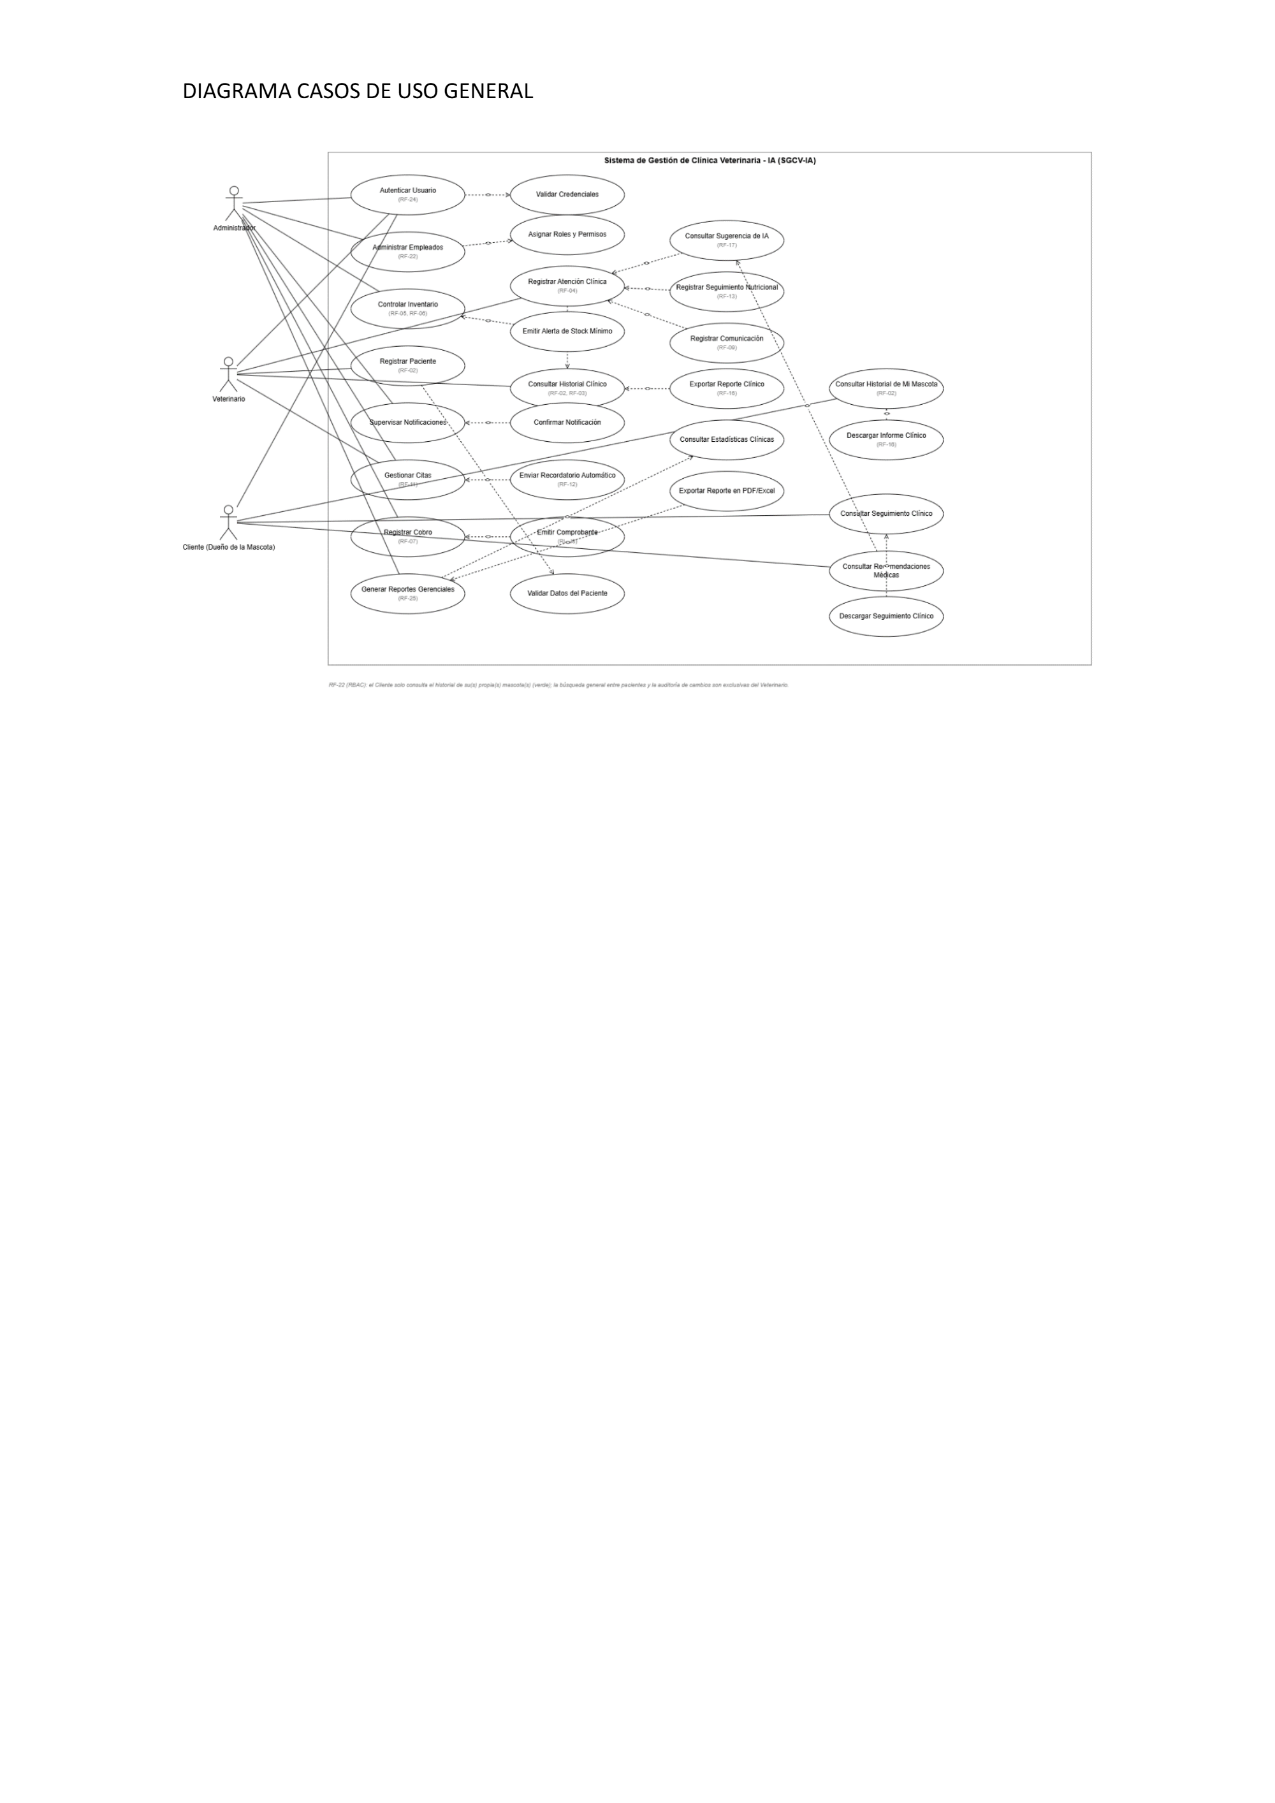
\includegraphics[width=5.79722in,height=3.42847in]{./media/image11.png}}{}}\label{section-1}

\section{}\label{section-2}

\section{}\label{section-3}

\section{}\label{section-4}

\section{}\label{section-5}

\section{}\label{section-6}

\section{}\label{section-7}

\section{}\label{section-8}

\section{}\label{section-9}

\subsubsection{Diagrama de Casos de Uso}\label{diagrama-de-casos-de-uso}

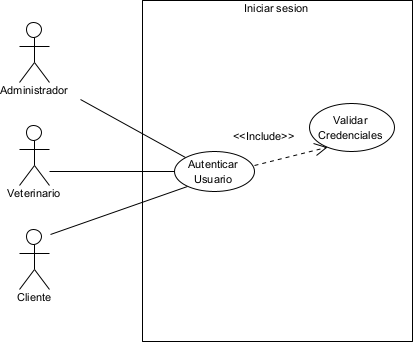
\includegraphics[width=4.30304in,height=3.5625in]{./media/image12.png}

\protect\phantomsection\label{_bookmark44}{}Ilustración 13. Caso de uso
Inicio sesión

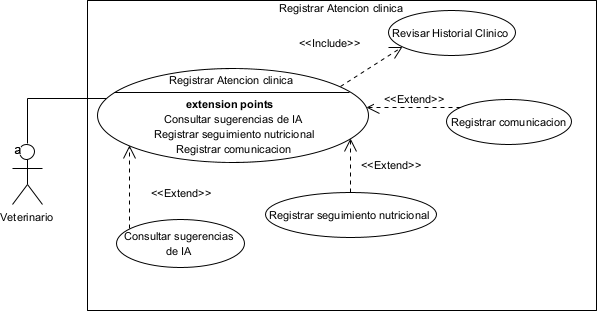
\includegraphics[width=5.72229in,height=2.98042in]{./media/image13.png}

\protect\phantomsection\label{_bookmark45}{}Ilustración 14. Caso de uso
Registrar atención clínica

\begin{quote}
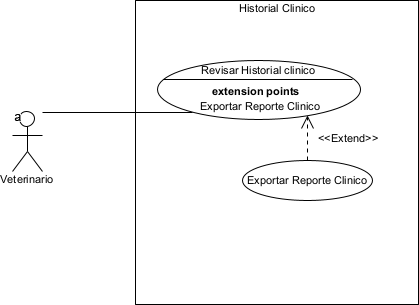
\includegraphics[width=4.36548in,height=3.17708in]{./media/image14.png}
\end{quote}

\protect\phantomsection\label{_bookmark46}{}Ilustración 15. Caso de uso
historial clínico

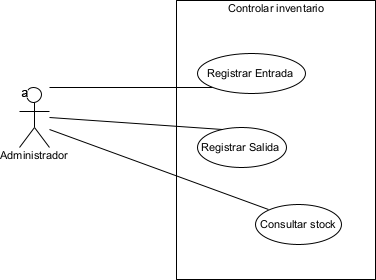
\includegraphics[width=3.91752in,height=2.91667in]{./media/image15.png}

\protect\phantomsection\label{_bookmark47}{}Ilustración 16. Caso de uso
Controlar inventario

\begin{quote}
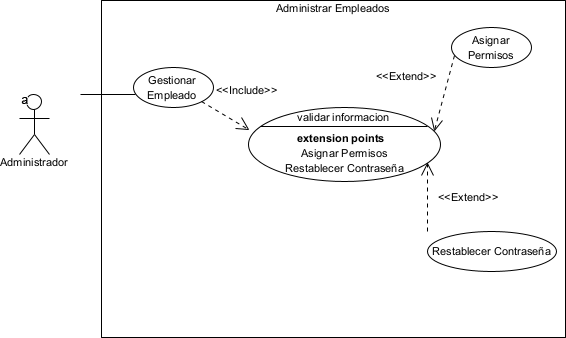
\includegraphics[width=5.66204in,height=3.38in]{./media/image16.png}
\end{quote}

\protect\phantomsection\label{_bookmark48}{}Ilustración 17. Caso de uso
Administrar Empleados

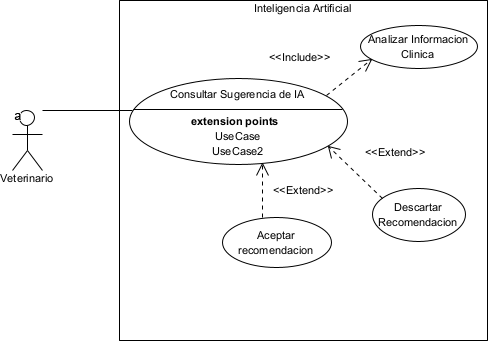
\includegraphics[width=5.08333in,height=3.55208in]{./media/image17.png}

\begin{quote}
\protect\phantomsection\label{_bookmark49}{}Ilustración 18. Cas de uso
Inteligencia Artificial

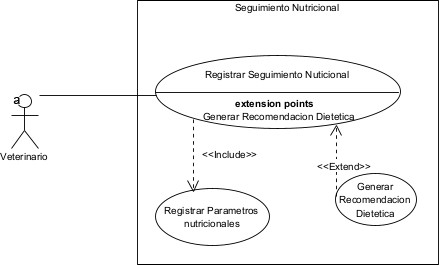
\includegraphics[width=4.57292in,height=2.76042in]{./media/image18.jpeg}
\end{quote}

\protect\phantomsection\label{_bookmark50}{}Ilustración 19. Caso de uso
Seguimiento Nutricional

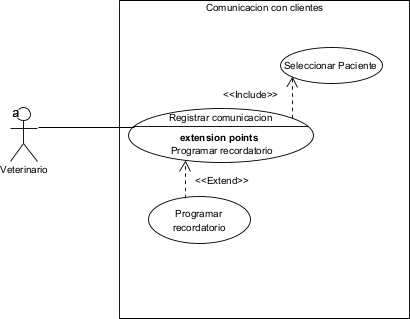
\includegraphics[width=2.94767in,height=2.29281in]{./media/image19.png}

\protect\phantomsection\label{_bookmark51}{}Ilustración 20. Caso de uso
Comunicación con cliente

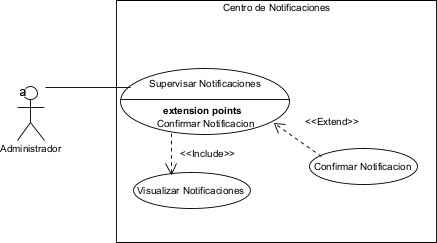
\includegraphics[width=4.55345in,height=2.53125in]{./media/image20.jpeg}

\protect\phantomsection\label{_bookmark52}{}Ilustración 21. Caso de uso
Centro de notificación

\paragraph{Caso de uso general del
SGCV-IA}\label{caso-de-uso-general-del-sgcv-ia}

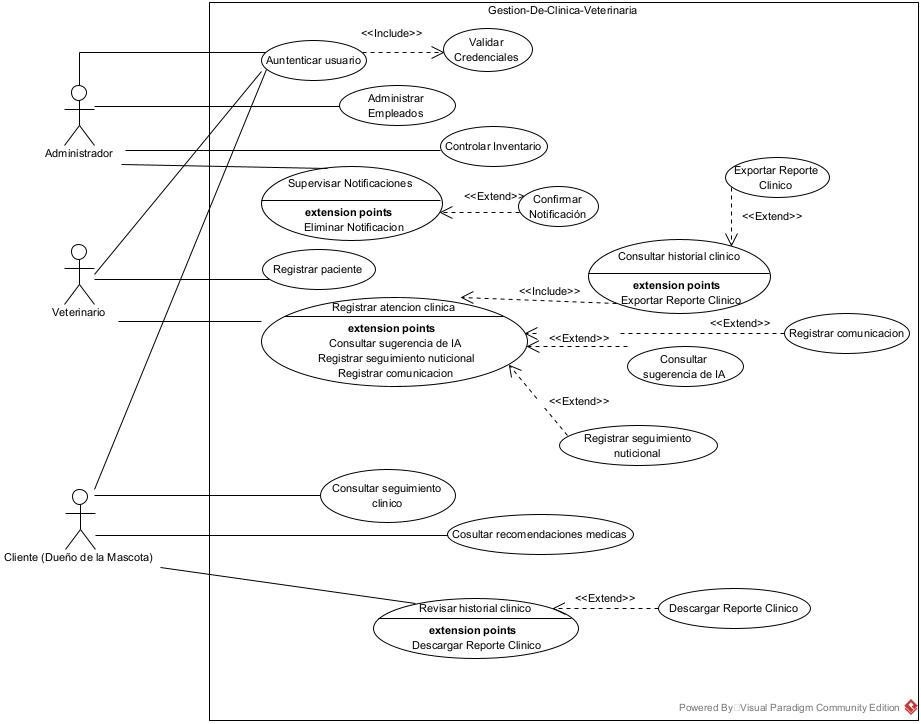
\includegraphics[width=5.85622in,height=4.60042in]{./media/image21.jpeg}

\begin{quote}
\protect\phantomsection\label{_bookmark53}{}Ilustración 22. Caso de uso
General
\end{quote}

\subsubsection{Especificación de Casos de
Uso}\label{especificaciuxf3n-de-casos-de-uso}

{\def\LTcaptype{none} % do not increment counter
\begin{longtable}[]{@{}
  >{\raggedright\arraybackslash}p{(\linewidth - 2\tabcolsep) * \real{0.3188}}
  >{\raggedright\arraybackslash}p{(\linewidth - 2\tabcolsep) * \real{0.5504}}@{}}
\toprule\noalign{}
\begin{minipage}[b]{\linewidth}\raggedright
CU-01--- Iniciar Sesión
\end{minipage} & \begin{minipage}[b]{\linewidth}\raggedright
\textbf{Actor principal:} Administrador, Veterinario y Cliente

\textbf{Actores secundarios:} Sistema de Autenticación
\textbf{Precondiciones:} El usuario debe estar registrado y su cuenta
debe encontrarse activa.

\textbf{Postcondiciones (éxito):} El usuario accede al sistema con los
permisos correspondientes a su rol. \textbf{Flujo principal:}

\begin{enumerate}
\def\labelenumi{\arabic{enumi}.}
\item
  El usuario accede a la página de inicio de sesión.
\item
  Ingresa su usuario y contraseña.
\item
  El sistema valida las credenciales.
\item
  El sistema identifica el rol del usuario.
\item
  El sistema concede el acceso y muestra el panel correspondiente.
\end{enumerate}
\end{minipage} \\
\midrule\noalign{}
\endhead
\bottomrule\noalign{}
\endlastfoot
\end{longtable}
}

{\def\LTcaptype{none} % do not increment counter
\begin{longtable}[]{@{}
  >{\raggedright\arraybackslash}p{(\linewidth - 2\tabcolsep) * \real{0.3188}}
  >{\raggedright\arraybackslash}p{(\linewidth - 2\tabcolsep) * \real{0.5504}}@{}}
\toprule\noalign{}
\begin{minipage}[b]{\linewidth}\raggedright
\end{minipage} & \begin{minipage}[b]{\linewidth}\raggedright
\textbf{Flujos alternativos:} A1: Credenciales incorrectas

→ El sistema informa el error y permite un nuevo intento.

A2: Campos obligatorios vacíos → El sistema solicita completar la
información.

A3: Cuenta inactiva → El sistema deniega el acceso.
\textbf{Postcondición (fallo):} El usuario no accede al sistema.
\end{minipage} \\
\midrule\noalign{}
\endhead
\bottomrule\noalign{}
\endlastfoot
\end{longtable}
}

{\def\LTcaptype{none} % do not increment counter
\begin{longtable}[]{@{}
  >{\raggedright\arraybackslash}p{(\linewidth - 2\tabcolsep) * \real{0.3188}}
  >{\raggedright\arraybackslash}p{(\linewidth - 2\tabcolsep) * \real{0.5504}}@{}}
\toprule\noalign{}
\begin{minipage}[b]{\linewidth}\raggedright
\textbf{CU-02 --- Registrar Atención Clínica}
\end{minipage} & \begin{minipage}[b]{\linewidth}\raggedright
\textbf{Actor principal:} Veterinario

\textbf{Actores secundarios:} Módulo de IA \textbf{Precondiciones:} El
veterinario ha iniciado sesión y el paciente se encuentra registrado.

\textbf{Postcondiciones (éxito):} La atención clínica queda registrada y
el historial del paciente es actualizado. \textbf{Flujo principal:}

\begin{enumerate}
\def\labelenumi{\arabic{enumi}.}
\item
  El veterinario accede al módulo de atención clínica.
\item
  Selecciona al paciente.
\item
  El sistema muestra el historial clínico.
\item
  El veterinario registra el diagnóstico y tratamiento.
\item
  El sistema valida la información.
\item
  El sistema actualiza el historial clínico. \textbf{Flujos
  alternativos:} A1: El veterinario solicita sugerencias de IA → El
  sistema presenta recomendaciones para apoyar el diagnóstico.
\end{enumerate}

A2: El veterinario registra un seguimiento nutricional

→ El sistema almacena la información correspondiente.

A3: El veterinario registra una comunicación con el dueño → El sistema
registra la comunicación en el historial.

A4: Información incompleta → El sistema solicita corregir los datos
antes de guardar.

\textbf{Postcondición (fallo):} La atención clínica no es registrada.
\end{minipage} \\
\midrule\noalign{}
\endhead
\bottomrule\noalign{}
\endlastfoot
\end{longtable}
}

{\def\LTcaptype{none} % do not increment counter
\begin{longtable}[]{@{}
  >{\raggedright\arraybackslash}p{(\linewidth - 2\tabcolsep) * \real{0.4347}}
  >{\raggedright\arraybackslash}p{(\linewidth - 2\tabcolsep) * \real{0.4345}}@{}}
\toprule\noalign{}
\begin{minipage}[b]{\linewidth}\raggedright
CU-03 --- Revisar Historial Clínico
\end{minipage} & \begin{minipage}[b]{\linewidth}\raggedright
\textbf{Actor principal:} Veterinario

\textbf{Actores secundarios:} Ninguno \textbf{Precondiciones:} El
paciente debe estar registrado en el sistema.

\textbf{Postcondiciones (éxito):} El historial clínico es consultado
correctamente.
\end{minipage} \\
\midrule\noalign{}
\endhead
\bottomrule\noalign{}
\endlastfoot
\end{longtable}
}

{\def\LTcaptype{none} % do not increment counter
\begin{longtable}[]{@{}
  >{\raggedright\arraybackslash}p{(\linewidth - 2\tabcolsep) * \real{0.4347}}
  >{\raggedright\arraybackslash}p{(\linewidth - 2\tabcolsep) * \real{0.4345}}@{}}
\toprule\noalign{}
\begin{minipage}[b]{\linewidth}\raggedright
\end{minipage} & \begin{minipage}[b]{\linewidth}\raggedright
\textbf{Flujo principal:}

\begin{enumerate}
\def\labelenumi{\arabic{enumi}.}
\item
  El veterinario accede al módulo de historial clínico.
\item
  Busca al paciente.
\item
  El sistema muestra el historial clínico.
\item
  El veterinario revisa la información médica registrada.
\end{enumerate}

\textbf{Flujos alternativos:}

A1: El paciente no existe → El sistema informa que no se encontraron
registros. A2: El veterinario exporta el historial → El sistema genera
el reporte clínico.

\textbf{Postcondición (fallo):} No se muestra información del historial.
\end{minipage} \\
\midrule\noalign{}
\endhead
\bottomrule\noalign{}
\endlastfoot
\end{longtable}
}

{\def\LTcaptype{none} % do not increment counter
\begin{longtable}[]{@{}
  >{\raggedright\arraybackslash}p{(\linewidth - 2\tabcolsep) * \real{0.4347}}
  >{\raggedright\arraybackslash}p{(\linewidth - 2\tabcolsep) * \real{0.4345}}@{}}
\toprule\noalign{}
\begin{minipage}[b]{\linewidth}\raggedright
CU-04 --- Controlar Inventario
\end{minipage} & \begin{minipage}[b]{\linewidth}\raggedright
\textbf{Actor principal:} Administrador \textbf{Actores secundarios:}
Sistema de Notificaciones

\textbf{Precondiciones:} El administrador ha iniciado sesión.

\textbf{Postcondiciones (éxito):} El inventario queda actualizado.

\textbf{Flujo principal:}

\begin{enumerate}
\def\labelenumi{\arabic{enumi}.}
\item
  El administrador accede al módulo de inventario.
\item
  El sistema muestra los productos registrados.
\item
  El administrador registra una entrada o salida de productos.
\item
  El sistema actualiza el stock.
\item
  El sistema guarda los cambios realizados.
\end{enumerate}

\textbf{Flujos alternativos:}

A1: Stock insuficiente → El sistema rechaza la operación.

A2: Stock mínimo alcanzado → El sistema genera una alerta de
abastecimiento.

Postcondición (fallo): El inventario permanece sin cambios.
\end{minipage} \\
\midrule\noalign{}
\endhead
\bottomrule\noalign{}
\endlastfoot
\end{longtable}
}

{\def\LTcaptype{none} % do not increment counter
\begin{longtable}[]{@{}
  >{\raggedright\arraybackslash}p{(\linewidth - 2\tabcolsep) * \real{0.4347}}
  >{\raggedright\arraybackslash}p{(\linewidth - 2\tabcolsep) * \real{0.4345}}@{}}
\toprule\noalign{}
\begin{minipage}[b]{\linewidth}\raggedright
CU-05 --- Gestionar Empleados
\end{minipage} & \begin{minipage}[b]{\linewidth}\raggedright
\textbf{Actor principal:} Administrador \textbf{Actores secundarios:}
Ninguno \textbf{Precondiciones:} El administrador ha iniciado sesión.

\textbf{Postcondiciones (éxito):} La información del empleado queda
actualizada correctamente.
\end{minipage} \\
\midrule\noalign{}
\endhead
\bottomrule\noalign{}
\endlastfoot
\end{longtable}
}

{\def\LTcaptype{none} % do not increment counter
\begin{longtable}[]{@{}
  >{\raggedright\arraybackslash}p{(\linewidth - 2\tabcolsep) * \real{0.4347}}
  >{\raggedright\arraybackslash}p{(\linewidth - 2\tabcolsep) * \real{0.4345}}@{}}
\toprule\noalign{}
\begin{minipage}[b]{\linewidth}\raggedright
\end{minipage} & \begin{minipage}[b]{\linewidth}\raggedright
\textbf{Flujo principal}

\begin{enumerate}
\def\labelenumi{\arabic{enumi}.}
\item
  El administrador accede al módulo de gestión de personal.
\item
  Selecciona el empleado que desea administrar.
\item
  El sistema muestra la información del empleado.
\item
  El administrador realiza las modificaciones necesarias.
\item
  El sistema valida la información ingresada.
\item
  El sistema guarda los cambios realizados.
\end{enumerate}

\textbf{Flujos alternativos}

A1: El administrador asigna permisos al empleado → El sistema actualiza
el rol y los permisos correspondientes.

A2: El administrador restablece la contraseña del empleado → El sistema
genera una nueva contraseña o solicita definir una nueva.

A3: Información inválida → El sistema informa los errores encontrados y
solicita corregirlos.

\textbf{Postcondición (fallo):} Los cambios no son almacenados.
\end{minipage} \\
\midrule\noalign{}
\endhead
\bottomrule\noalign{}
\endlastfoot
\end{longtable}
}

\subsubsection{Diagrama de Clases
Conceptual}\label{diagrama-de-clases-conceptual}

{\def\LTcaptype{none} % do not increment counter
\begin{longtable}[]{@{}
  >{\raggedright\arraybackslash}p{(\linewidth - 4\tabcolsep) * \real{0.3191}}
  >{\raggedright\arraybackslash}p{(\linewidth - 4\tabcolsep) * \real{0.1536}}
  >{\raggedright\arraybackslash}p{(\linewidth - 4\tabcolsep) * \real{0.4058}}@{}}
\toprule\noalign{}
\multicolumn{3}{@{}>{\centering\arraybackslash}p{(\linewidth - 4\tabcolsep) * \real{0.8785} + 4\tabcolsep}@{}}{%
\begin{minipage}[b]{\linewidth}\centering
\textbf{Relaciones Principales y Multiplicidad}
\end{minipage}} \\
\midrule\noalign{}
\endhead
\bottomrule\noalign{}
\endlastfoot
\textbf{Relación} & \textbf{Multiplicidad} & \textbf{Justificación} \\
Usuario - Administrador & No aplica & Un administrador es un tipo de
usuario,

por lo que hereda sus atributos y características generales. \\
Usuario --- Veterinario & No aplica & Un veterinario es un tipo de
usuario, compartiendo la información común definida en la clase
Usuario. \\
Cliente --- Paciente & 1: N & Un cliente puede ser propietario de varias
mascotas, mientras que cada paciente

pertenece a un único cliente. \\
Paciente --- Historial & 1: 1 & Cada paciente posee un único historial

clínico, el cual no puede existir sin el paciente. \\
Paciente --- Atención Clínica & 1: N & Un paciente puede recibir
múltiples atenciones clínicas a lo largo del tiempo, pero cada atención
corresponde a un

único paciente. \\
Historial Clínico --- Atención Clínica & 1: N & Un historial clínico
almacena todas las atenciones realizadas al paciente y estas no tienen
sentido sin el historial al que

pertenecen. \\
\end{longtable}
}

{\def\LTcaptype{none} % do not increment counter
\begin{longtable}[]{@{}
  >{\raggedright\arraybackslash}p{(\linewidth - 4\tabcolsep) * \real{0.3191}}
  >{\raggedright\arraybackslash}p{(\linewidth - 4\tabcolsep) * \real{0.1536}}
  >{\raggedright\arraybackslash}p{(\linewidth - 4\tabcolsep) * \real{0.4058}}@{}}
\toprule\noalign{}
\begin{minipage}[b]{\linewidth}\raggedright
Veterinario --- Atención Clínica
\end{minipage} & \begin{minipage}[b]{\linewidth}\raggedright
1: N
\end{minipage} & \begin{minipage}[b]{\linewidth}\raggedright
Un veterinario puede realizar numerosas atenciones clínicas, mientras
que cada

atención es realizada por un único veterinario
\end{minipage} \\
\midrule\noalign{}
\endhead
\bottomrule\noalign{}
\endlastfoot
Administrador --- Inventario & 1: 1 & El administrador supervisa el
inventario del sistema, siendo responsable de su

gestión y actualización. \\
Inventario --- Producto & 1: N & Un inventario administra múltiples
productos. Los productos pueden existir independientemente del
inventario, por lo

que no existe dependencia de vida. \\
Inventario --- Notificación & 1: N & El inventario puede generar
múltiples notificaciones relacionadas con bajo stock

o vencimiento de productos, dependiendo de su estado. \\
\end{longtable}
}

\protect\phantomsection\label{_bookmark56}{}Tabla 11. Relaciones
principales y multiplicidad del diagrama de clases

\textbf{Diagramas de actividad}

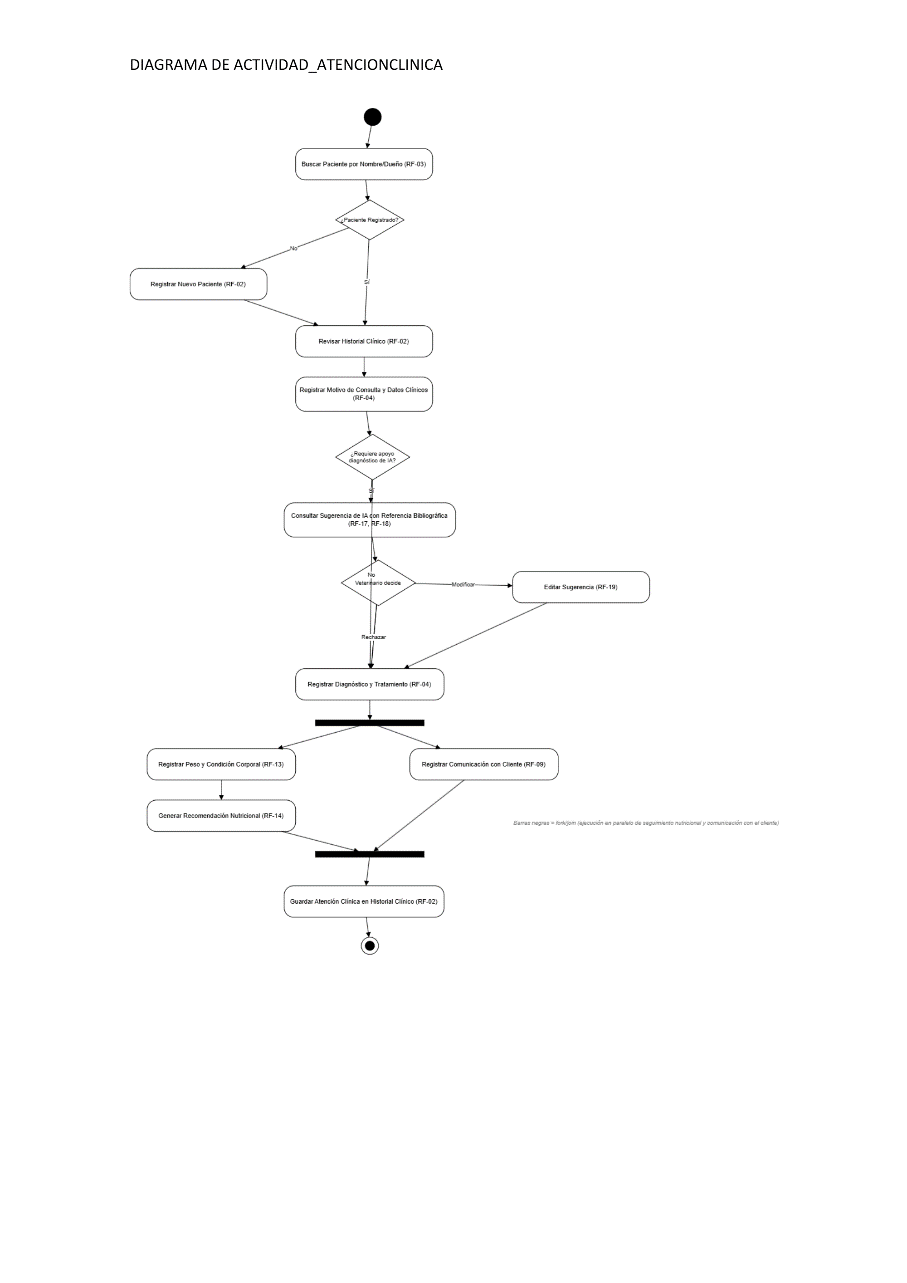
\includegraphics[width=4.11905in,height=4.56797in]{./media/image22.png}

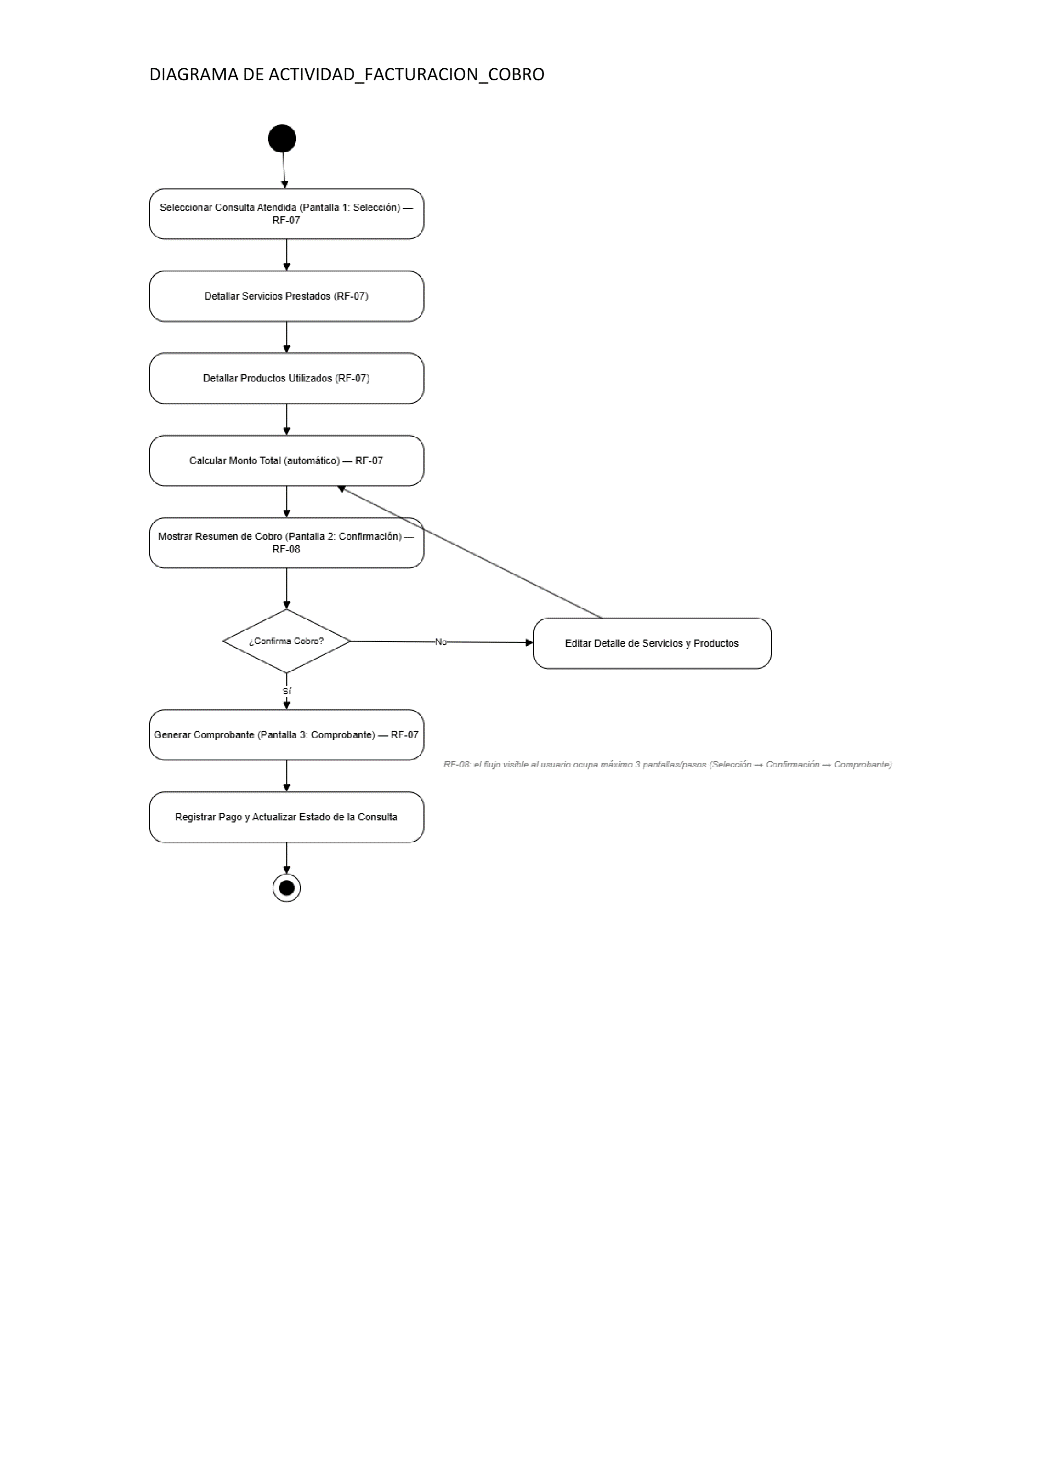
\includegraphics[width=4.72619in,height=4.33874in]{./media/image23.png}

\subsubsection{Diagrama de clase}\label{diagrama-de-clase}

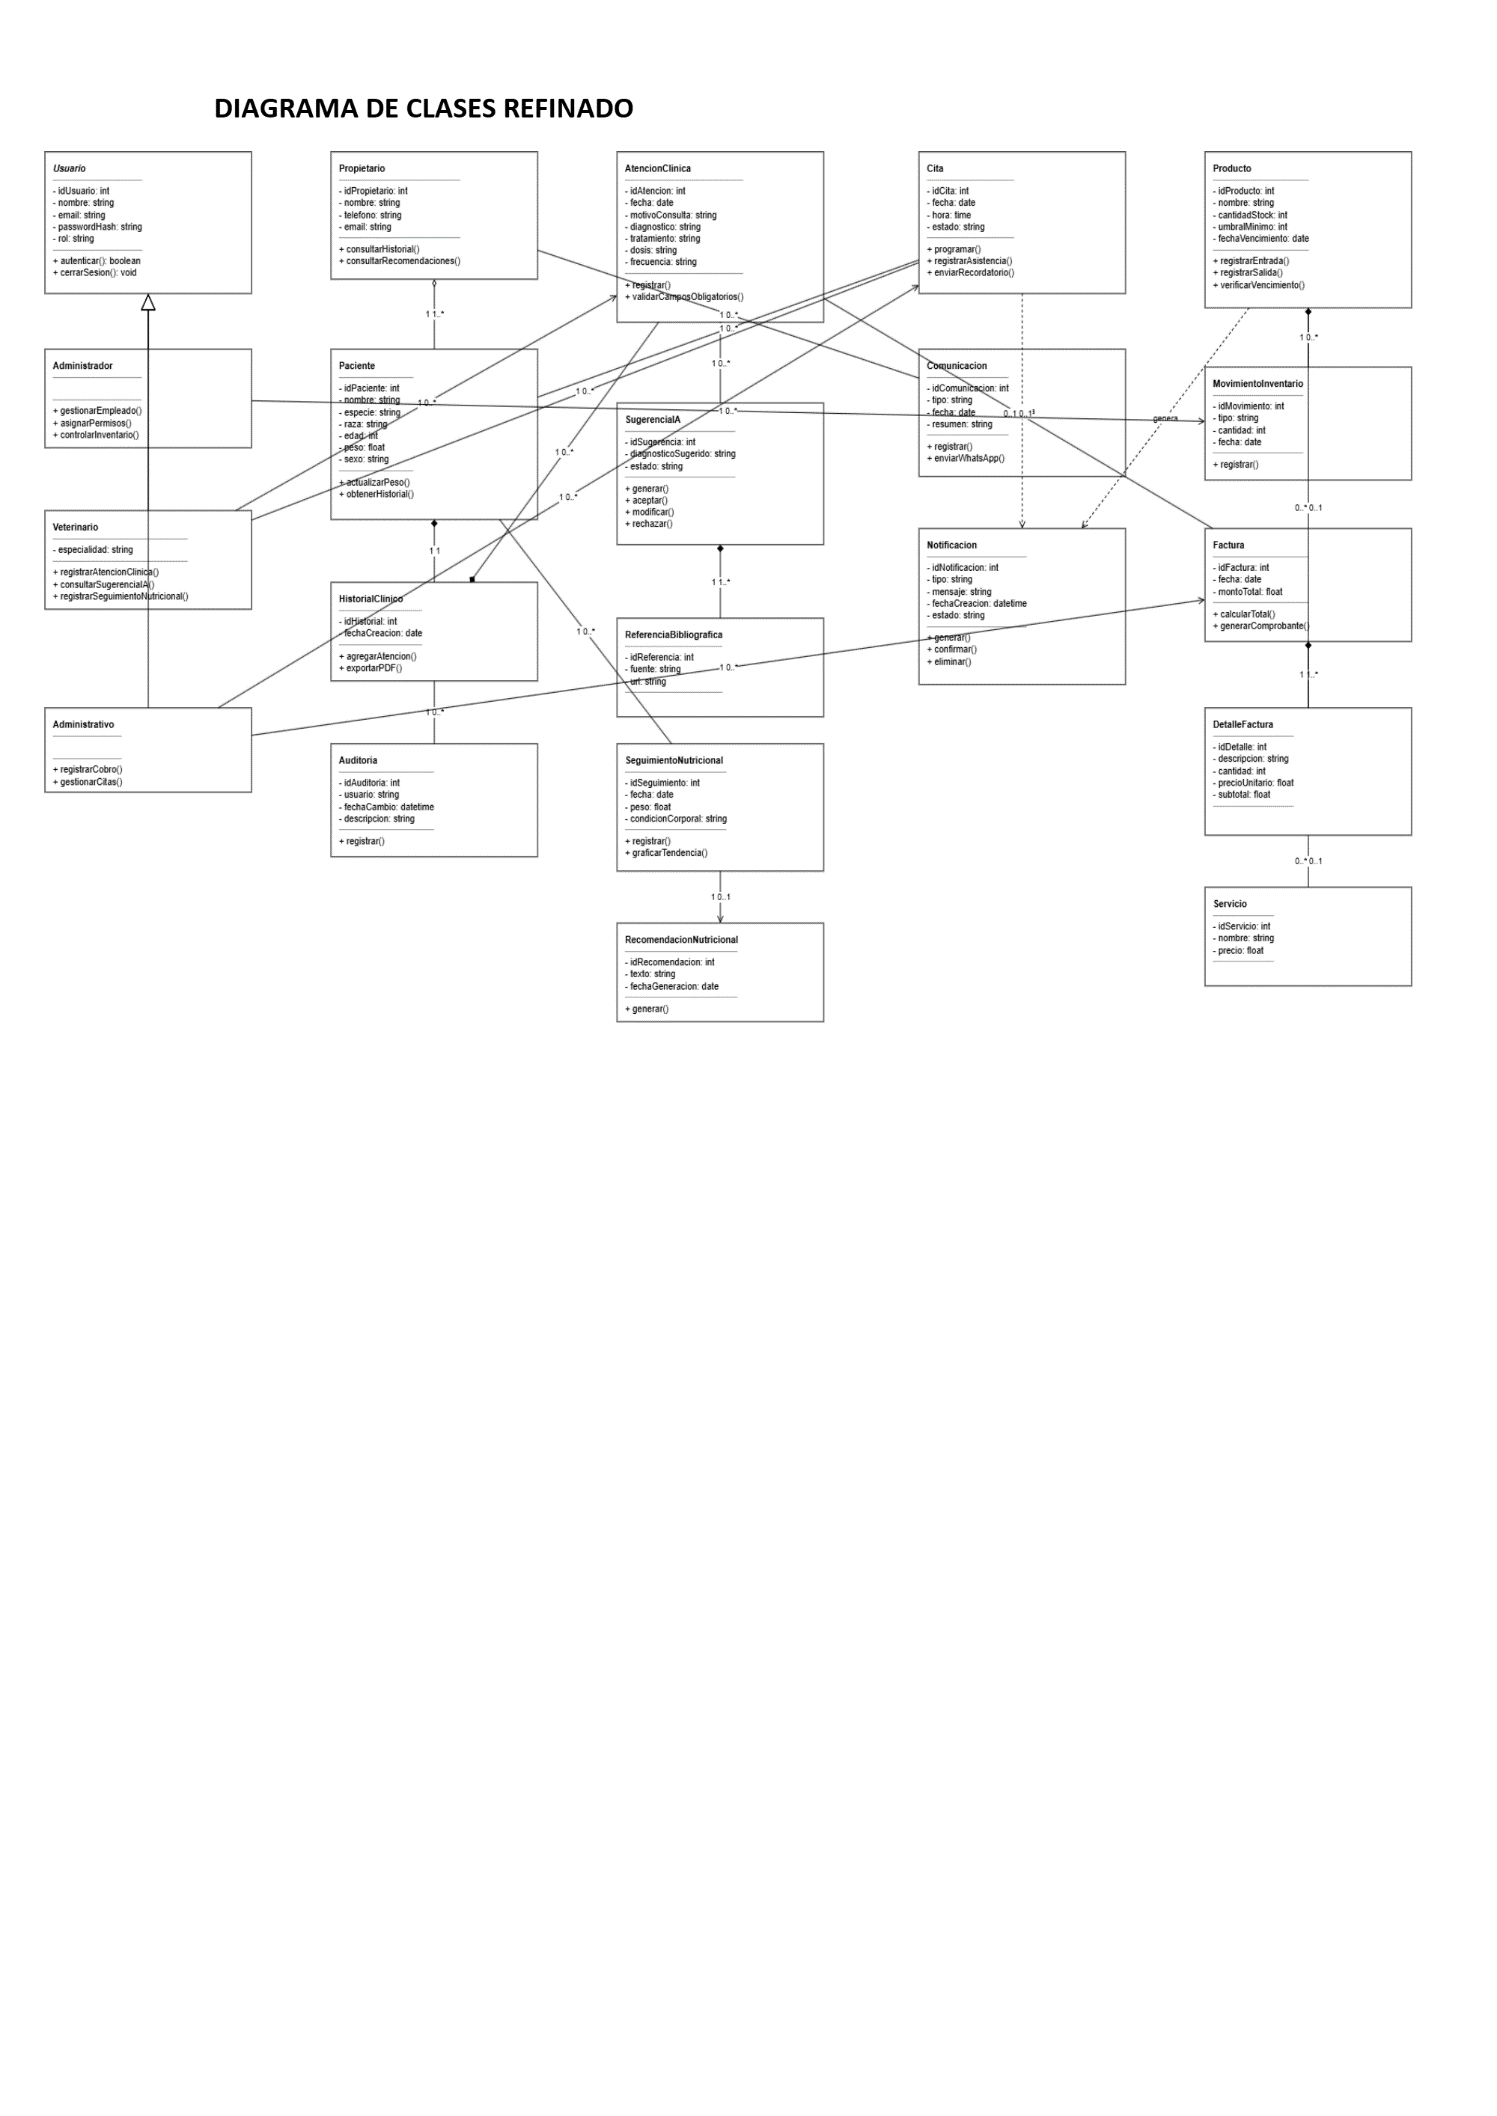
\includegraphics[width=6.79514in,height=5.0119in]{./media/image24.png}

\protect\phantomsection\label{_bookmark57}{}\emph{\textbf{Ilustración
23. Diagrama de clases}}

\textbf{Diagrama de componentes}

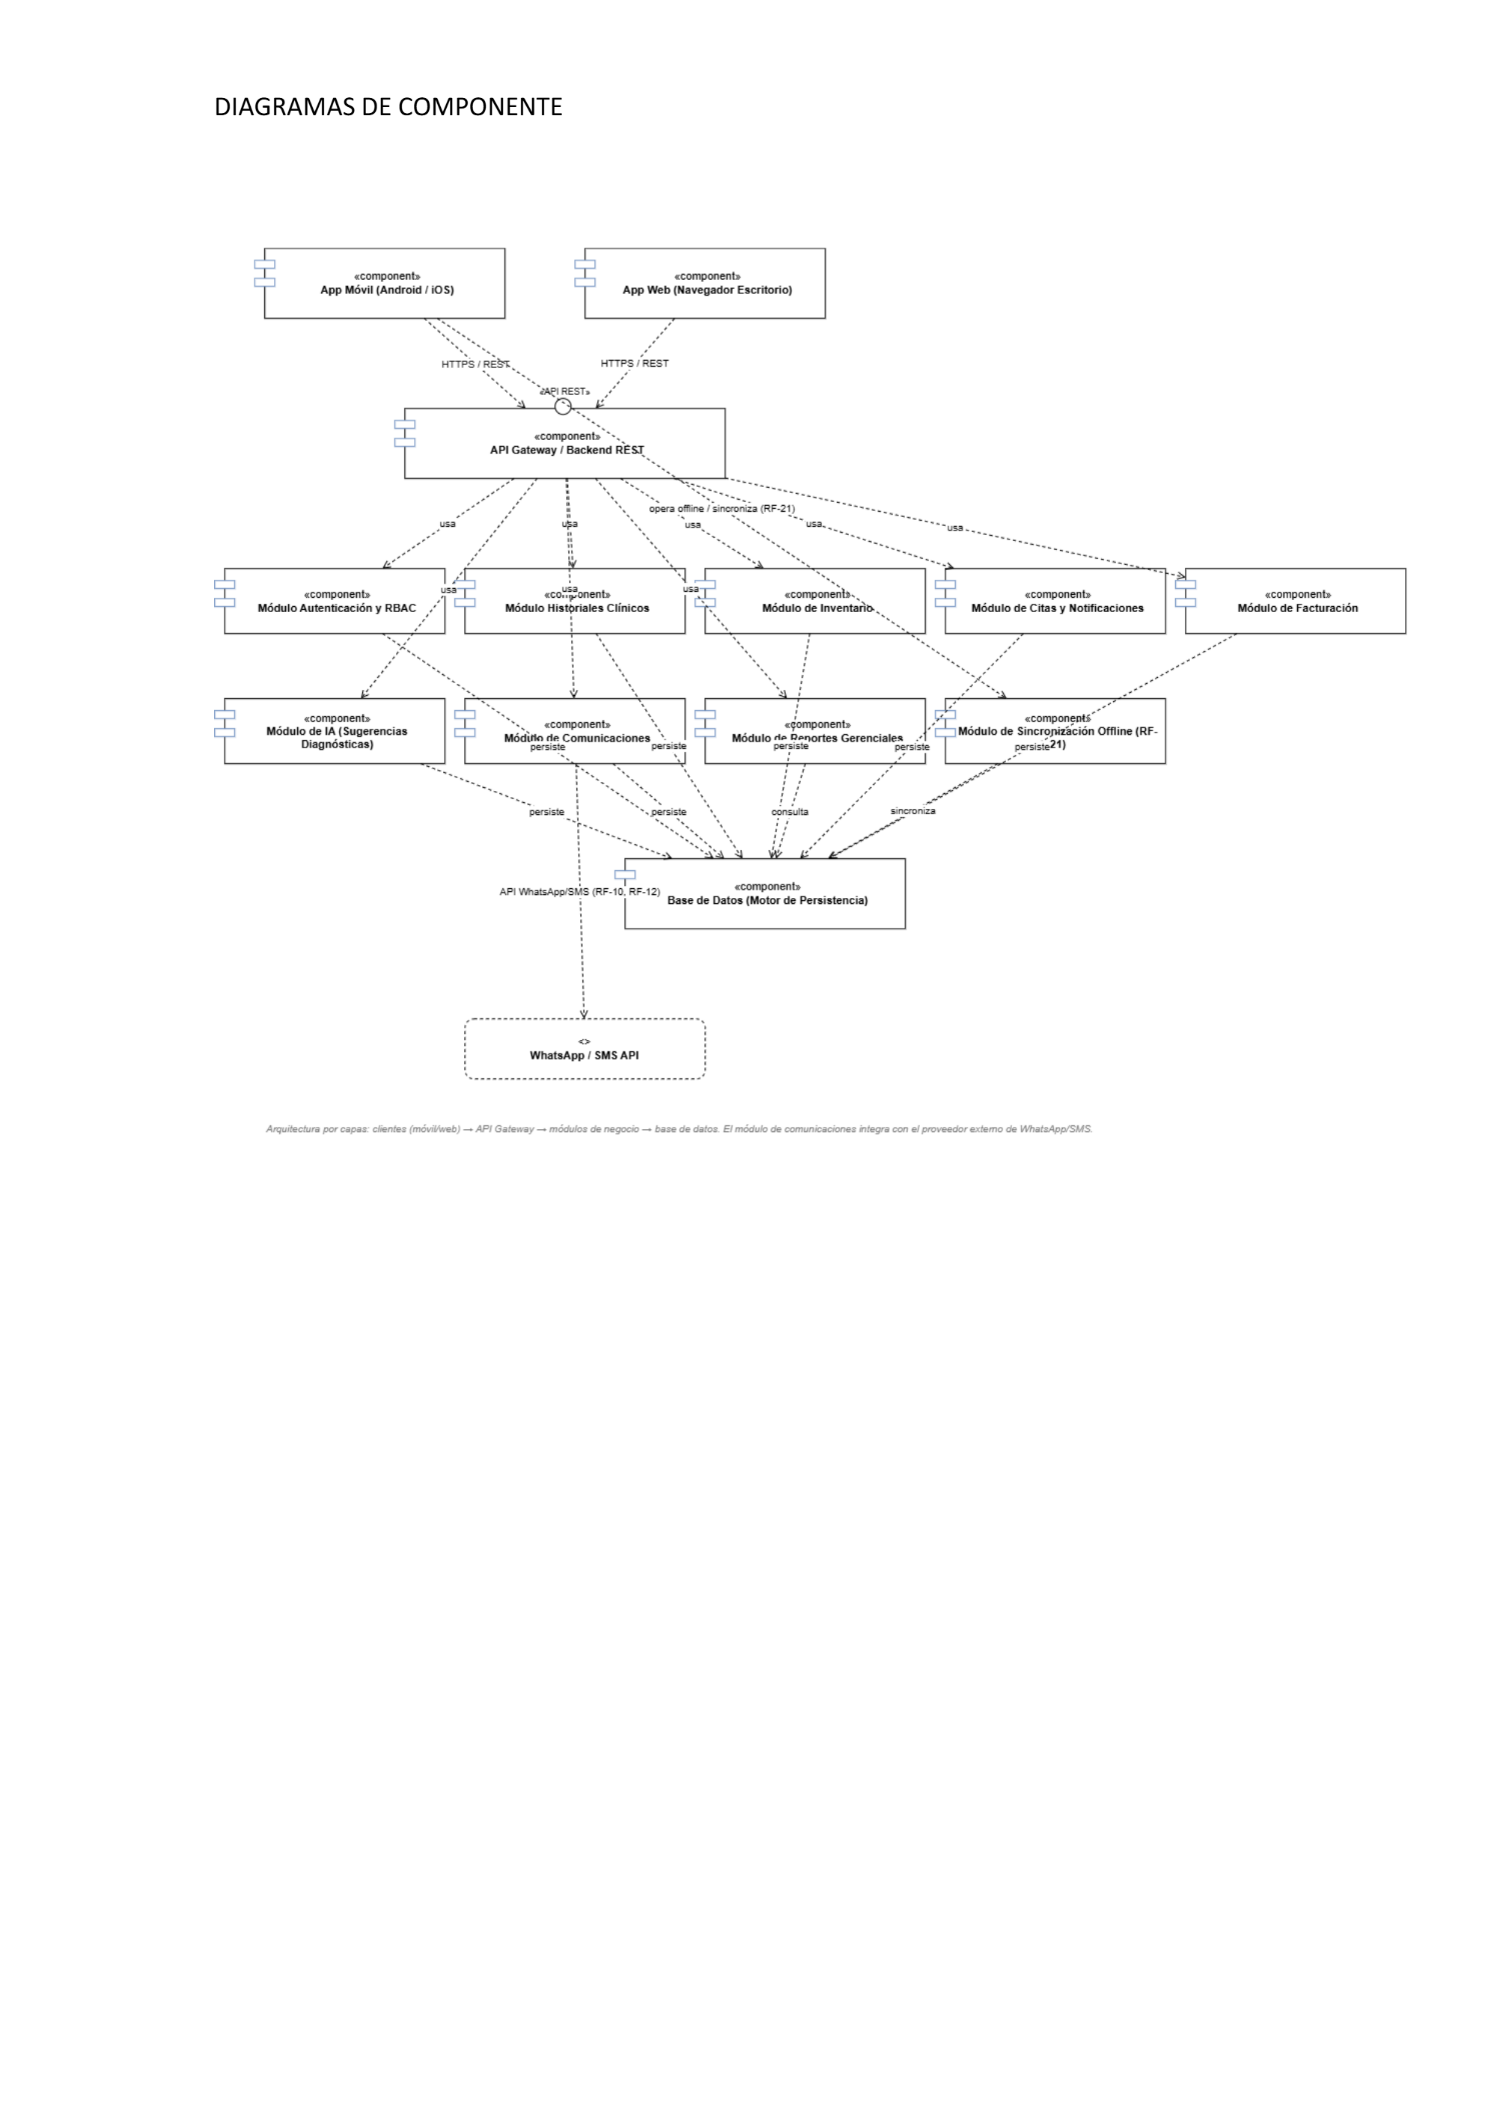
\includegraphics[width=6.79514in,height=5.79762in]{./media/image25.png}

\textbf{Diagrama de despliegue}

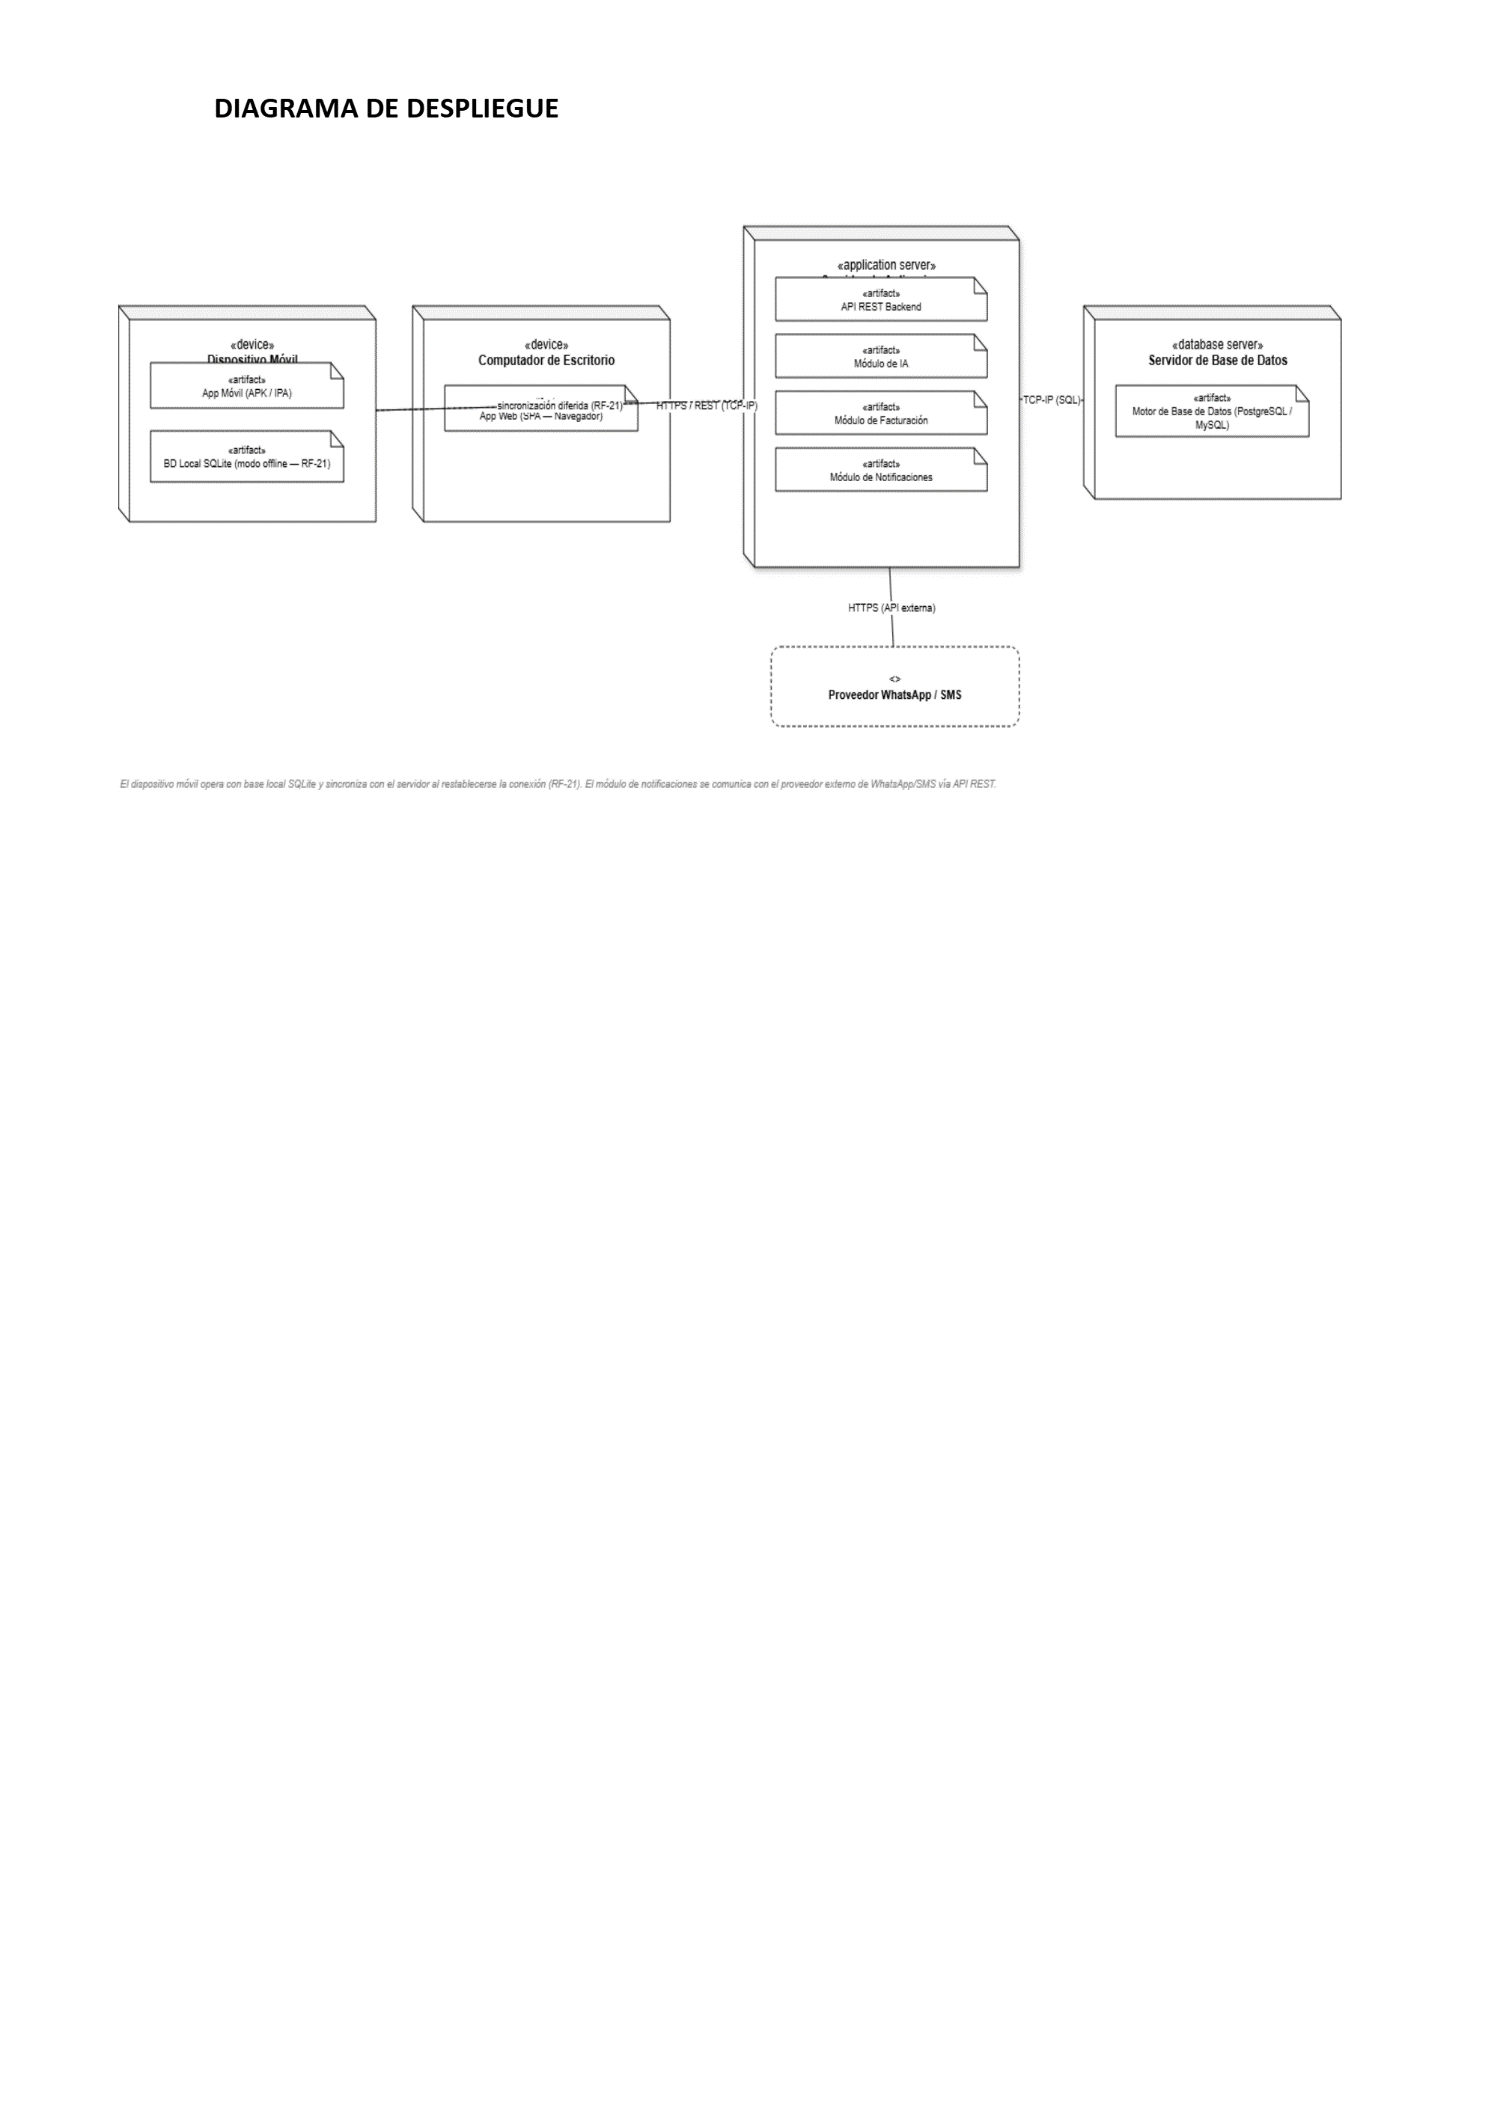
\includegraphics[width=6.79514in,height=3.69048in]{./media/image26.png}

\textbf{Diagrama de esatdo}

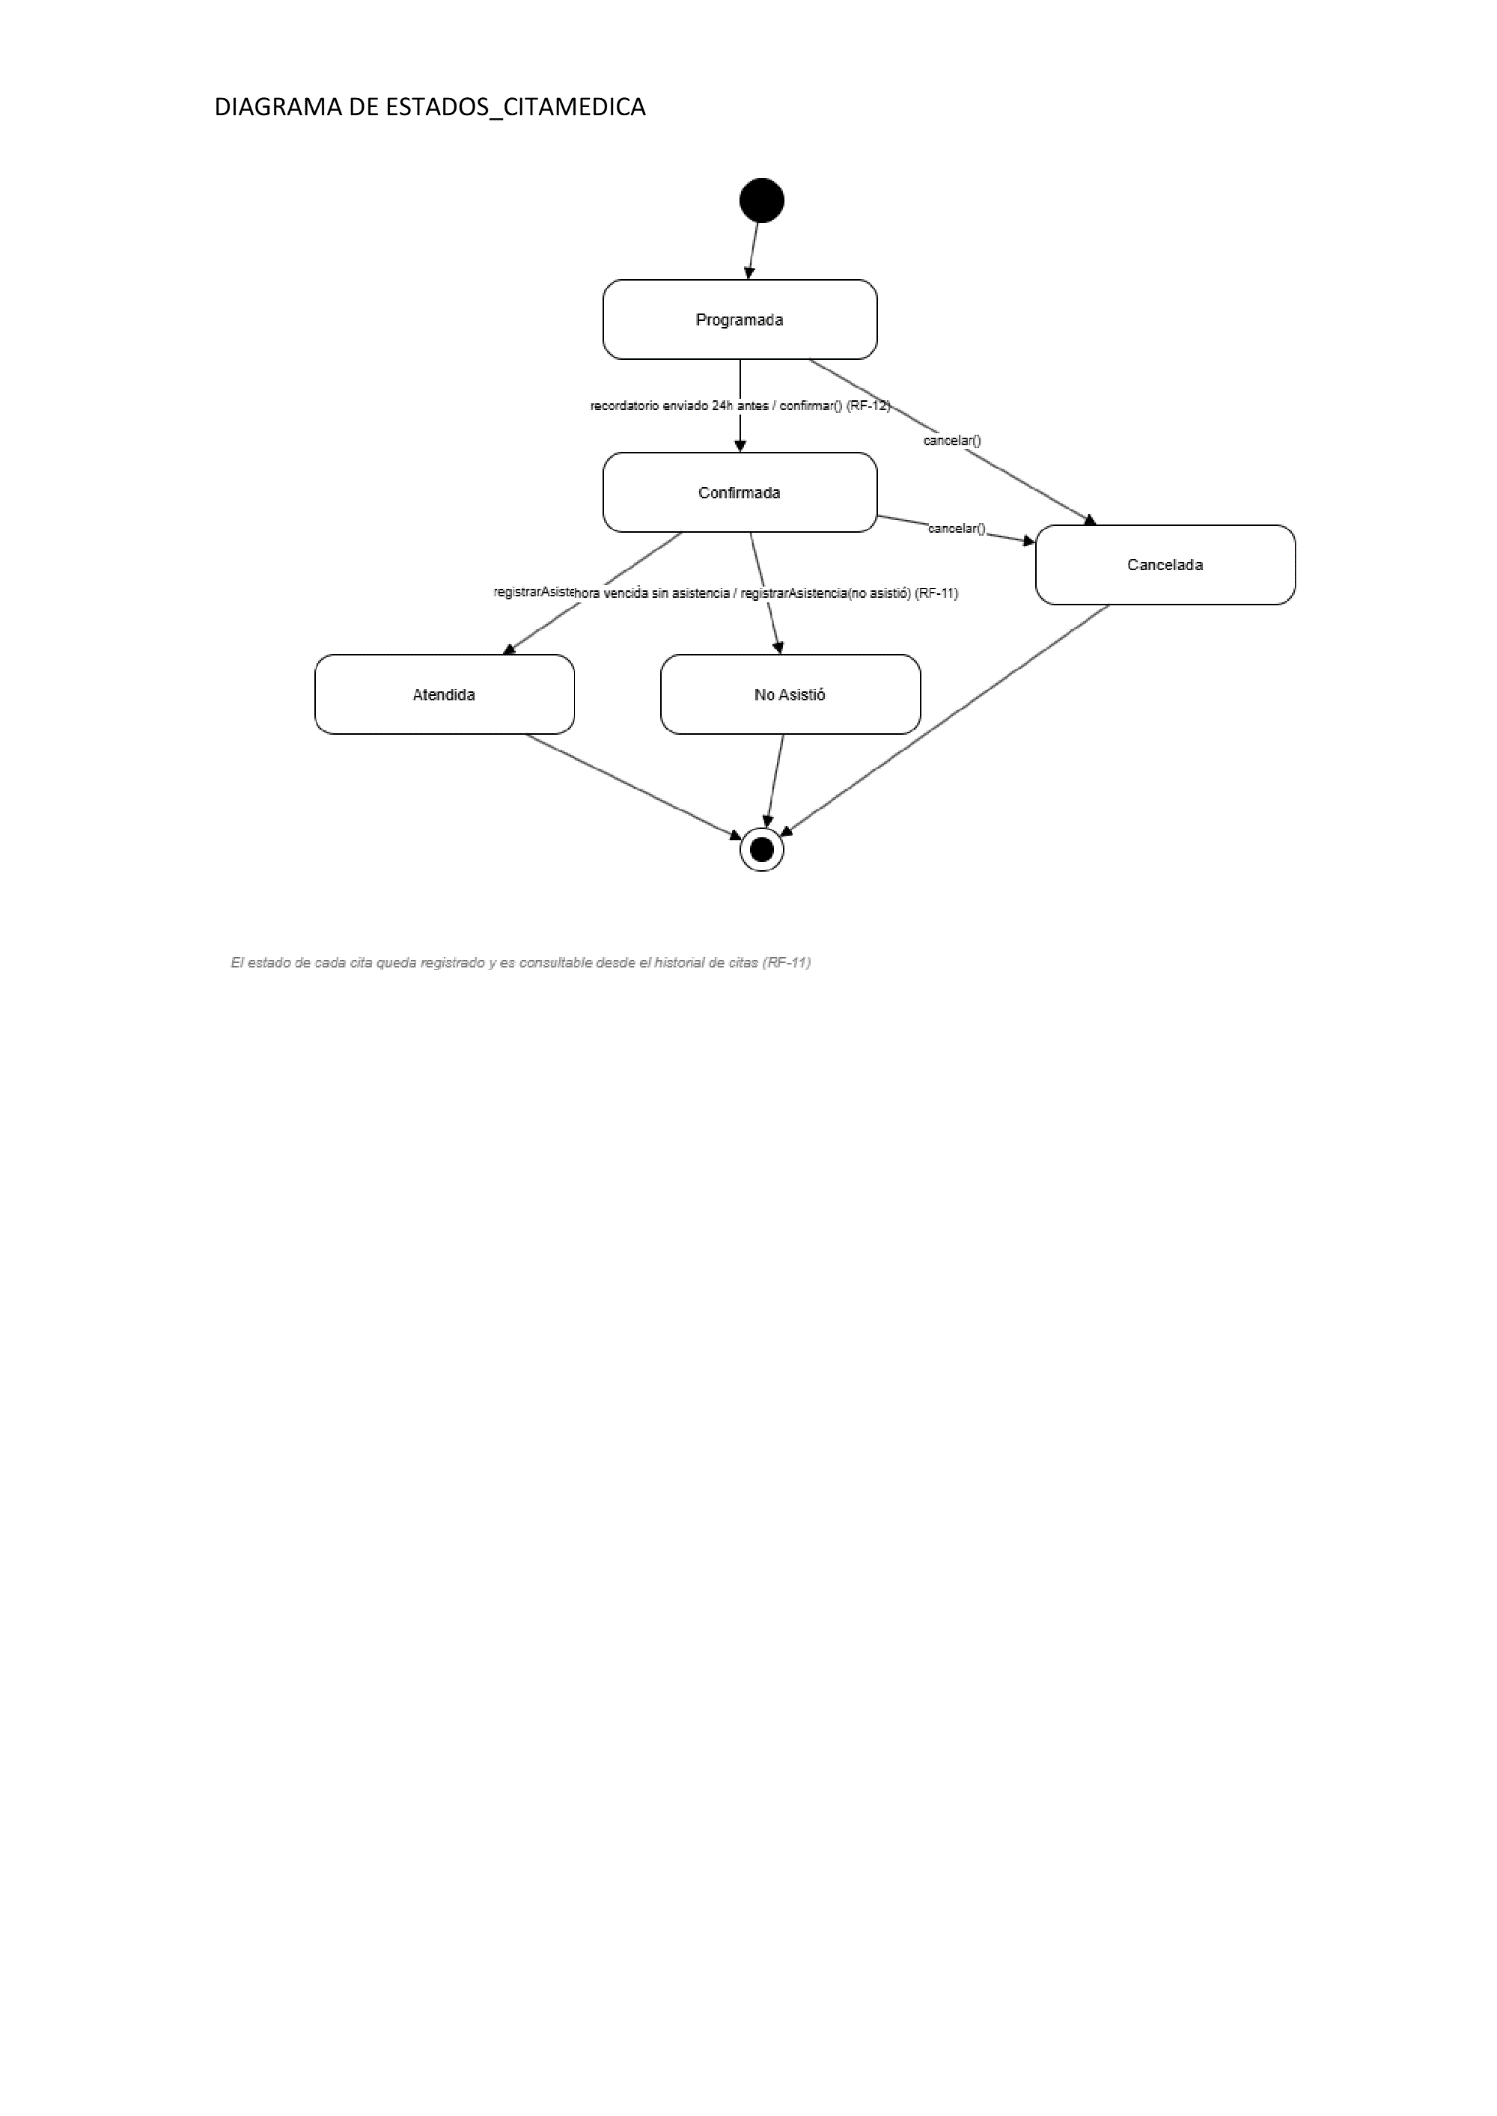
\includegraphics[width=6.79514in,height=5.07143in]{./media/image27.png}

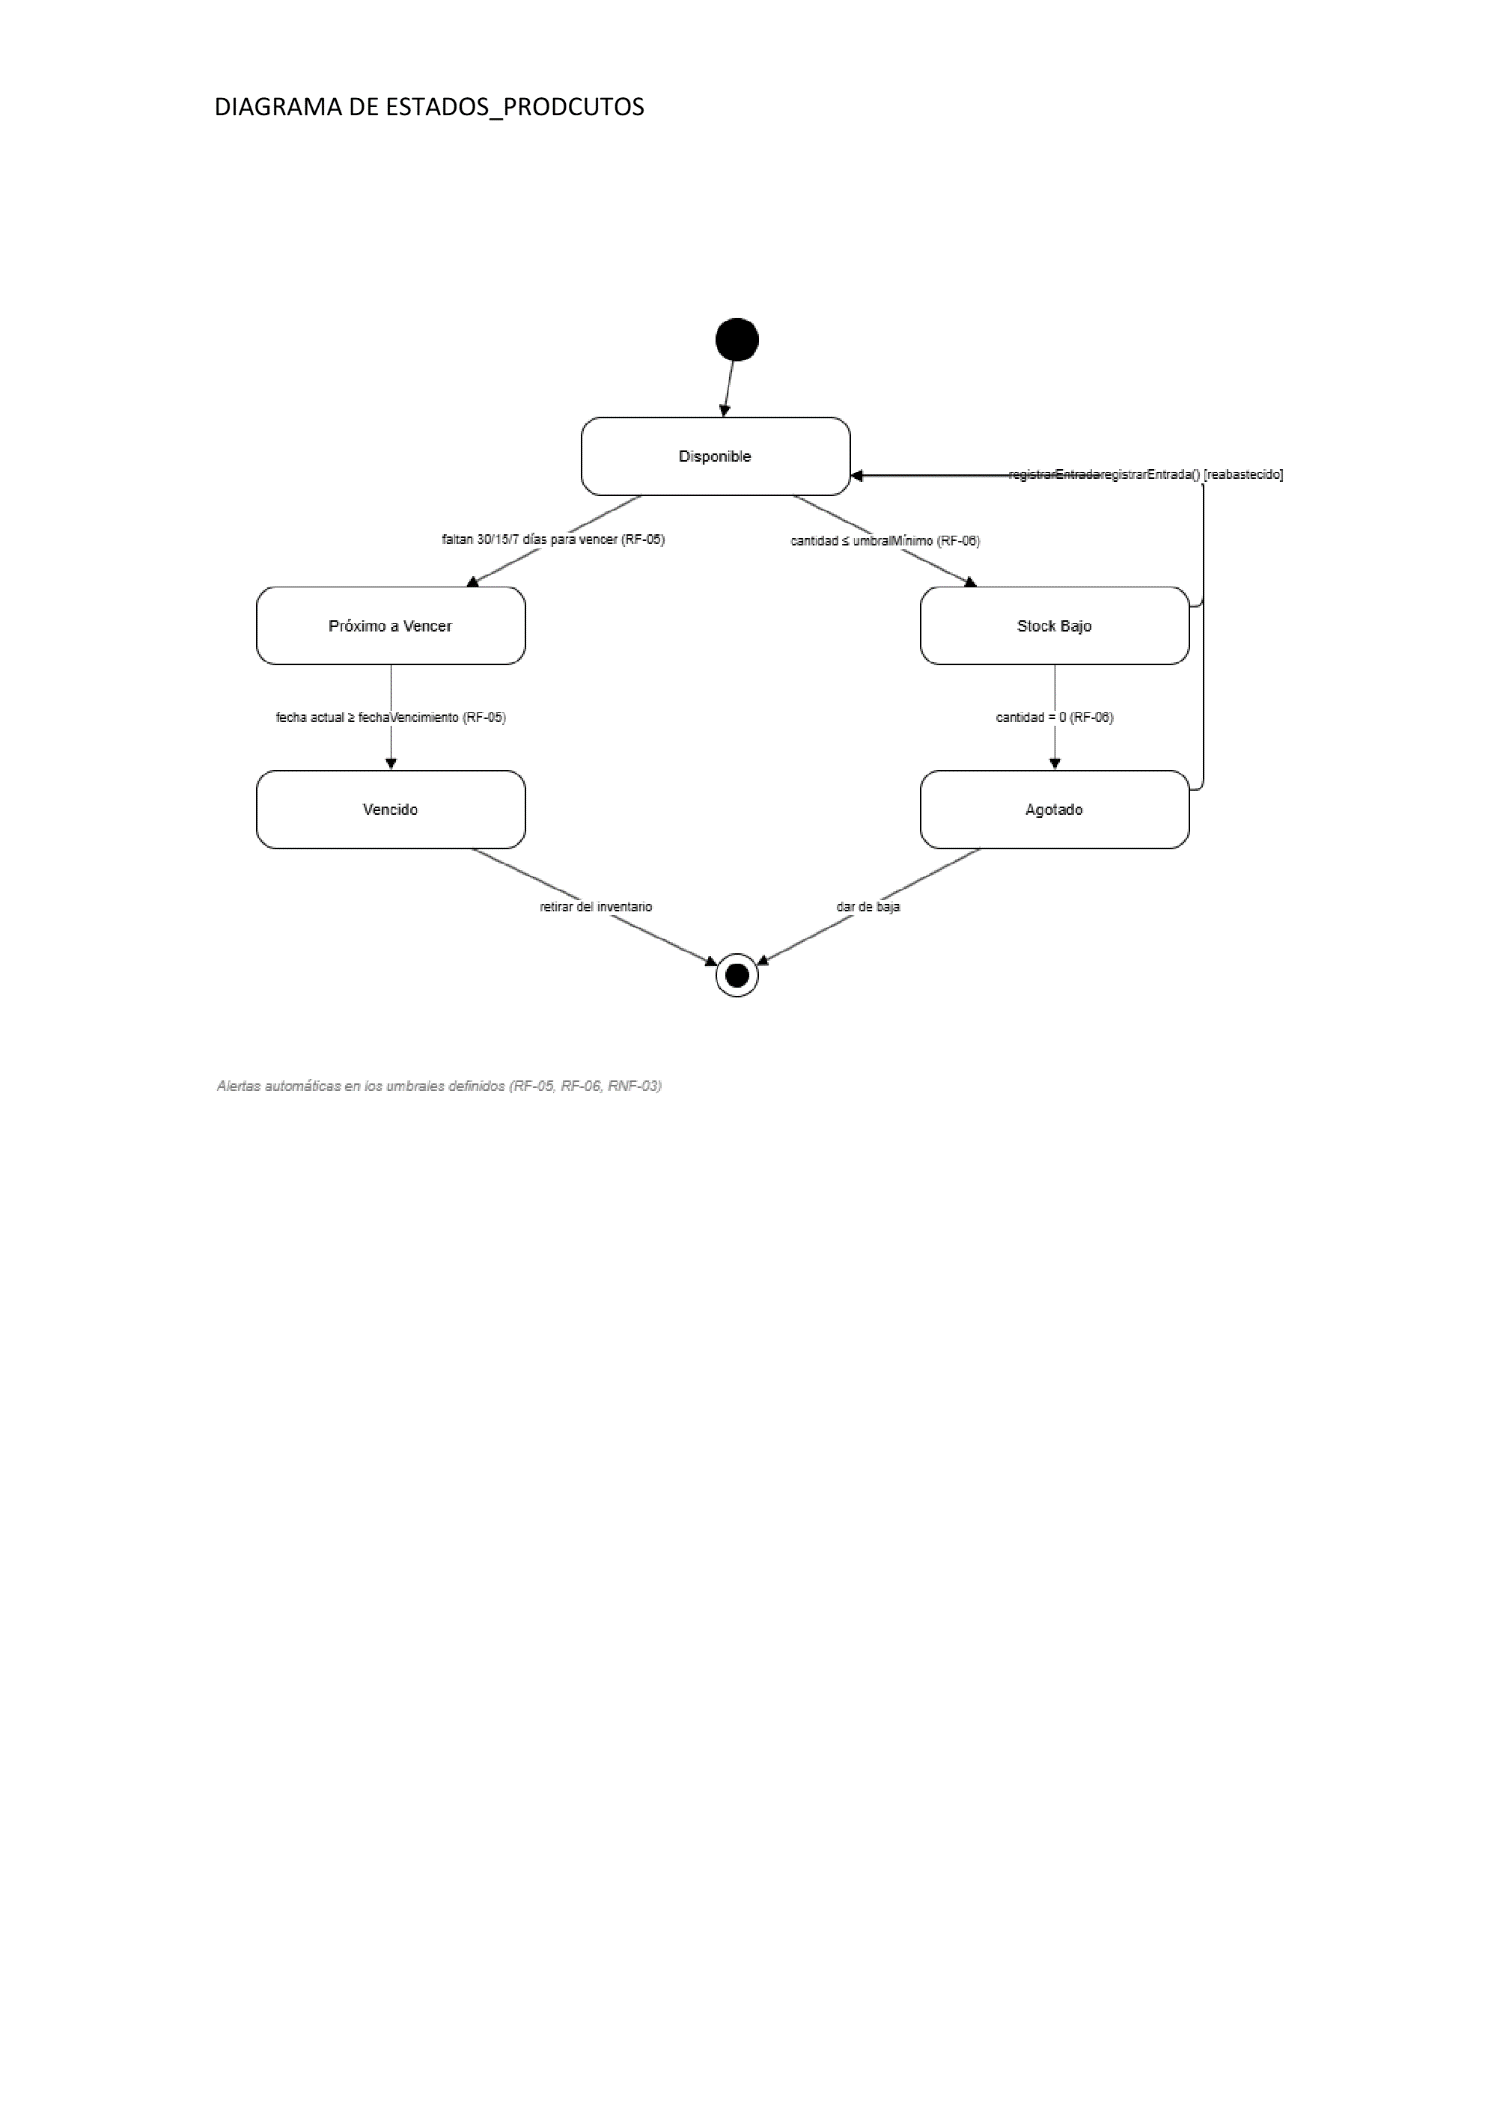
\includegraphics[width=6.79514in,height=5.30952in]{./media/image28.png}

\textbf{Diagrama de secuencias}

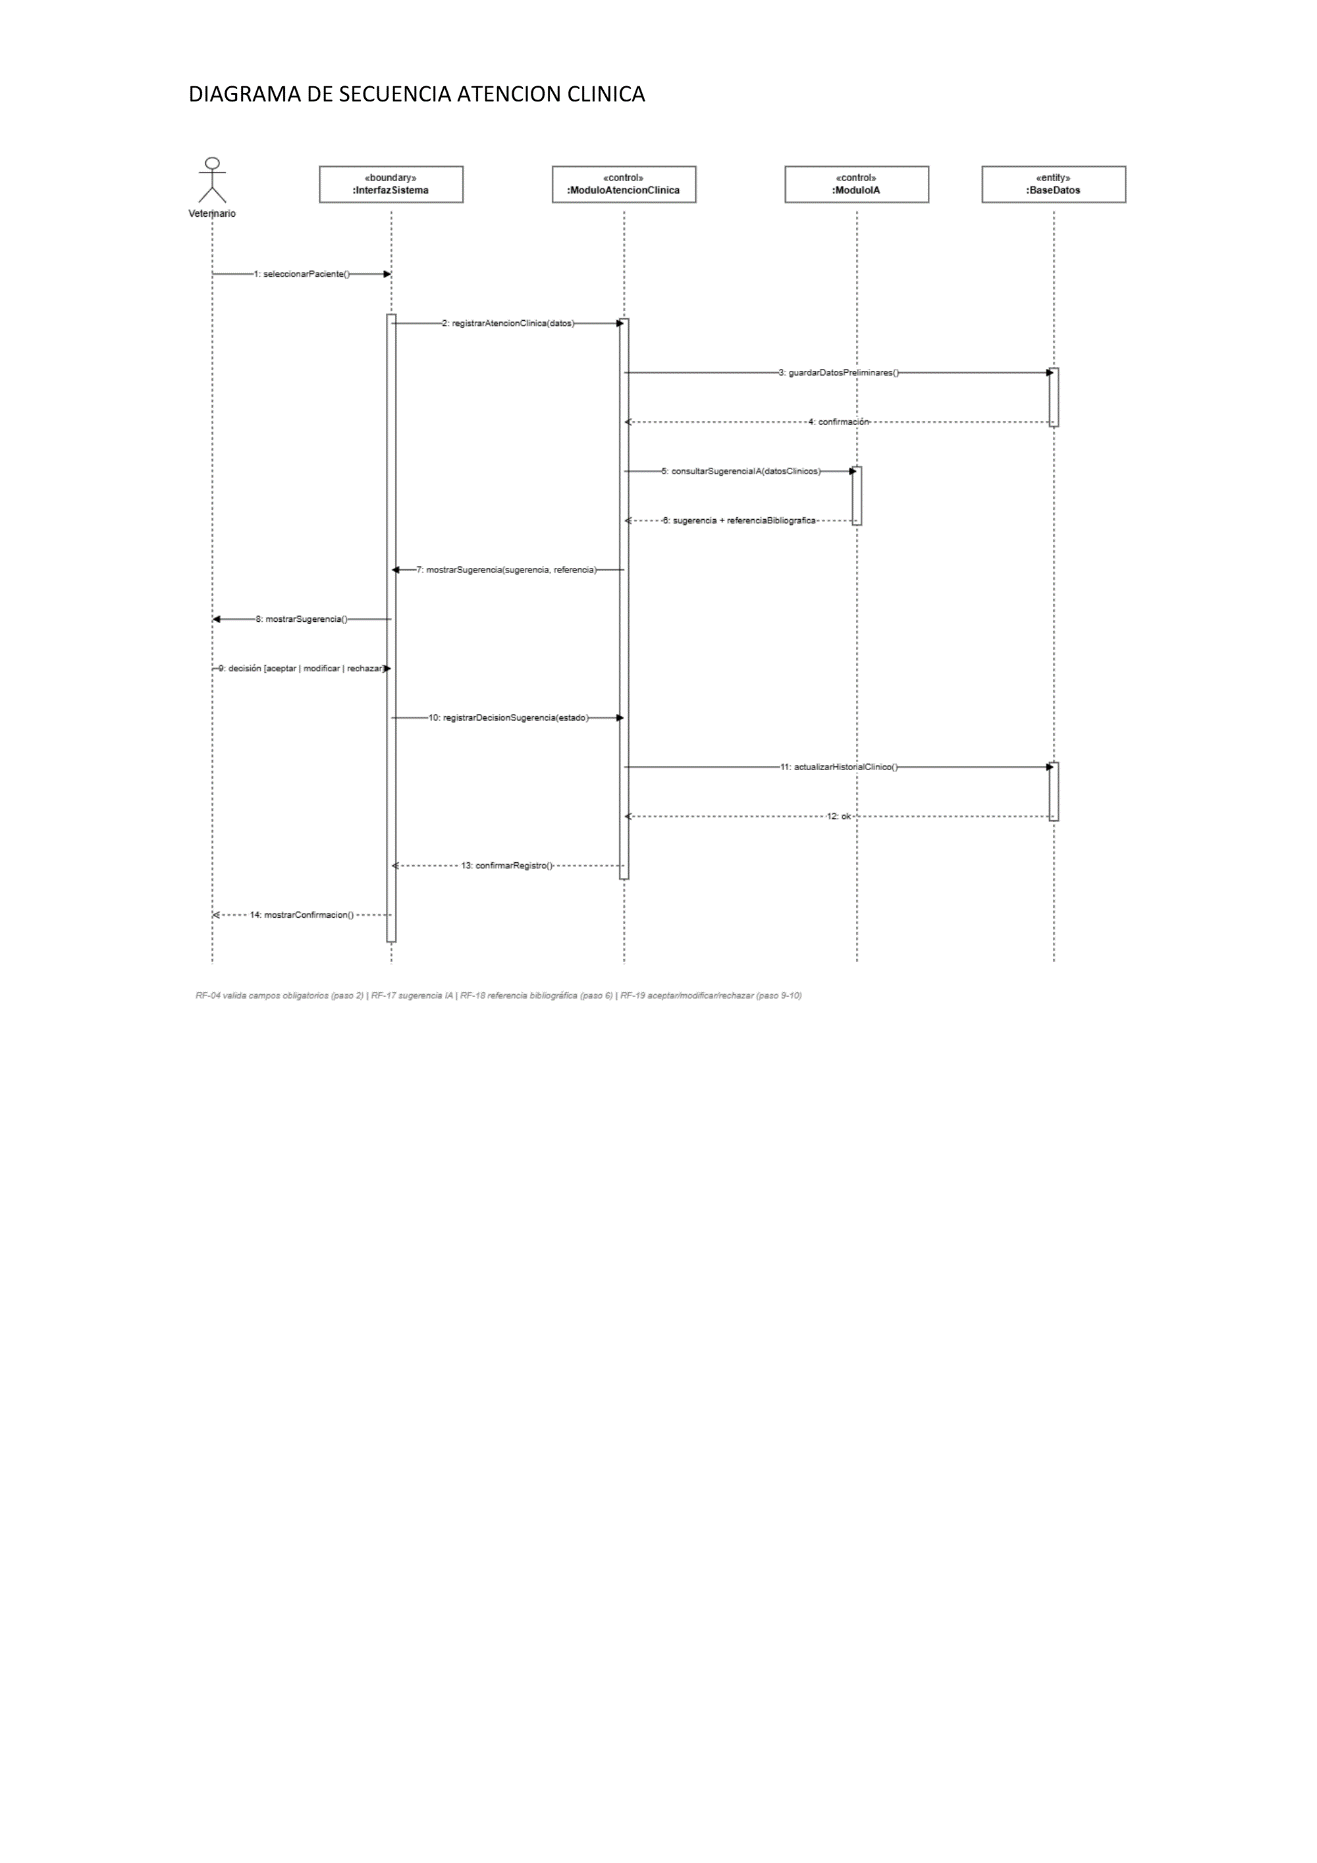
\includegraphics[width=5.98809in,height=4.92021in]{./media/image29.png}

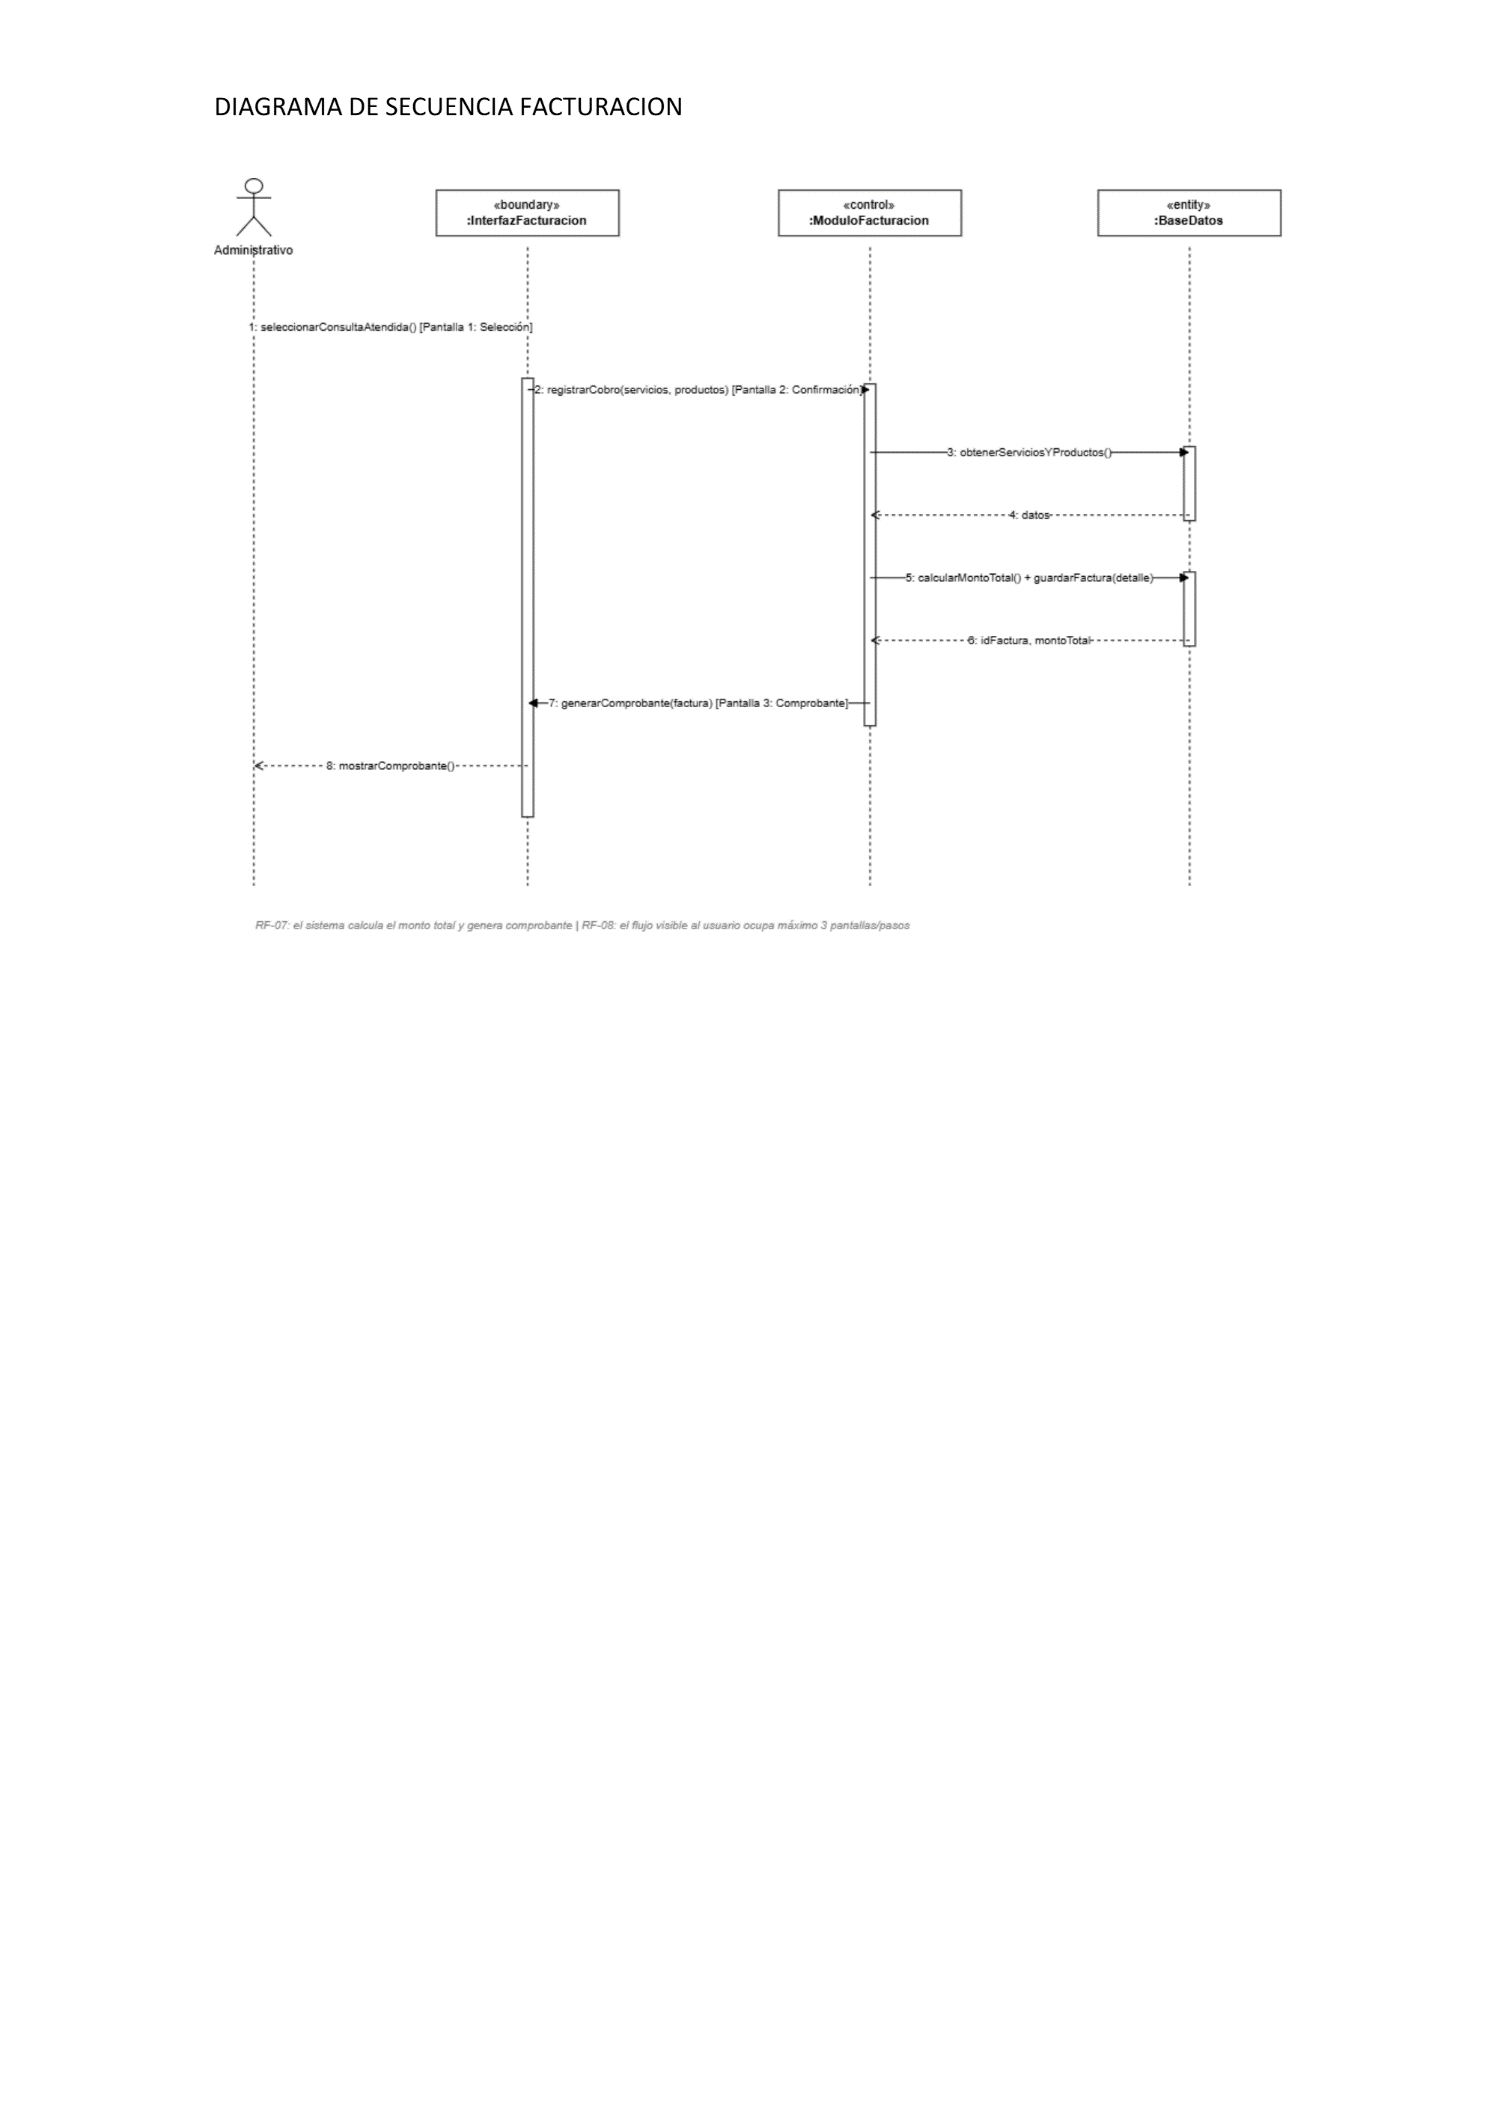
\includegraphics[width=6.79514in,height=4.64286in]{./media/image30.png}

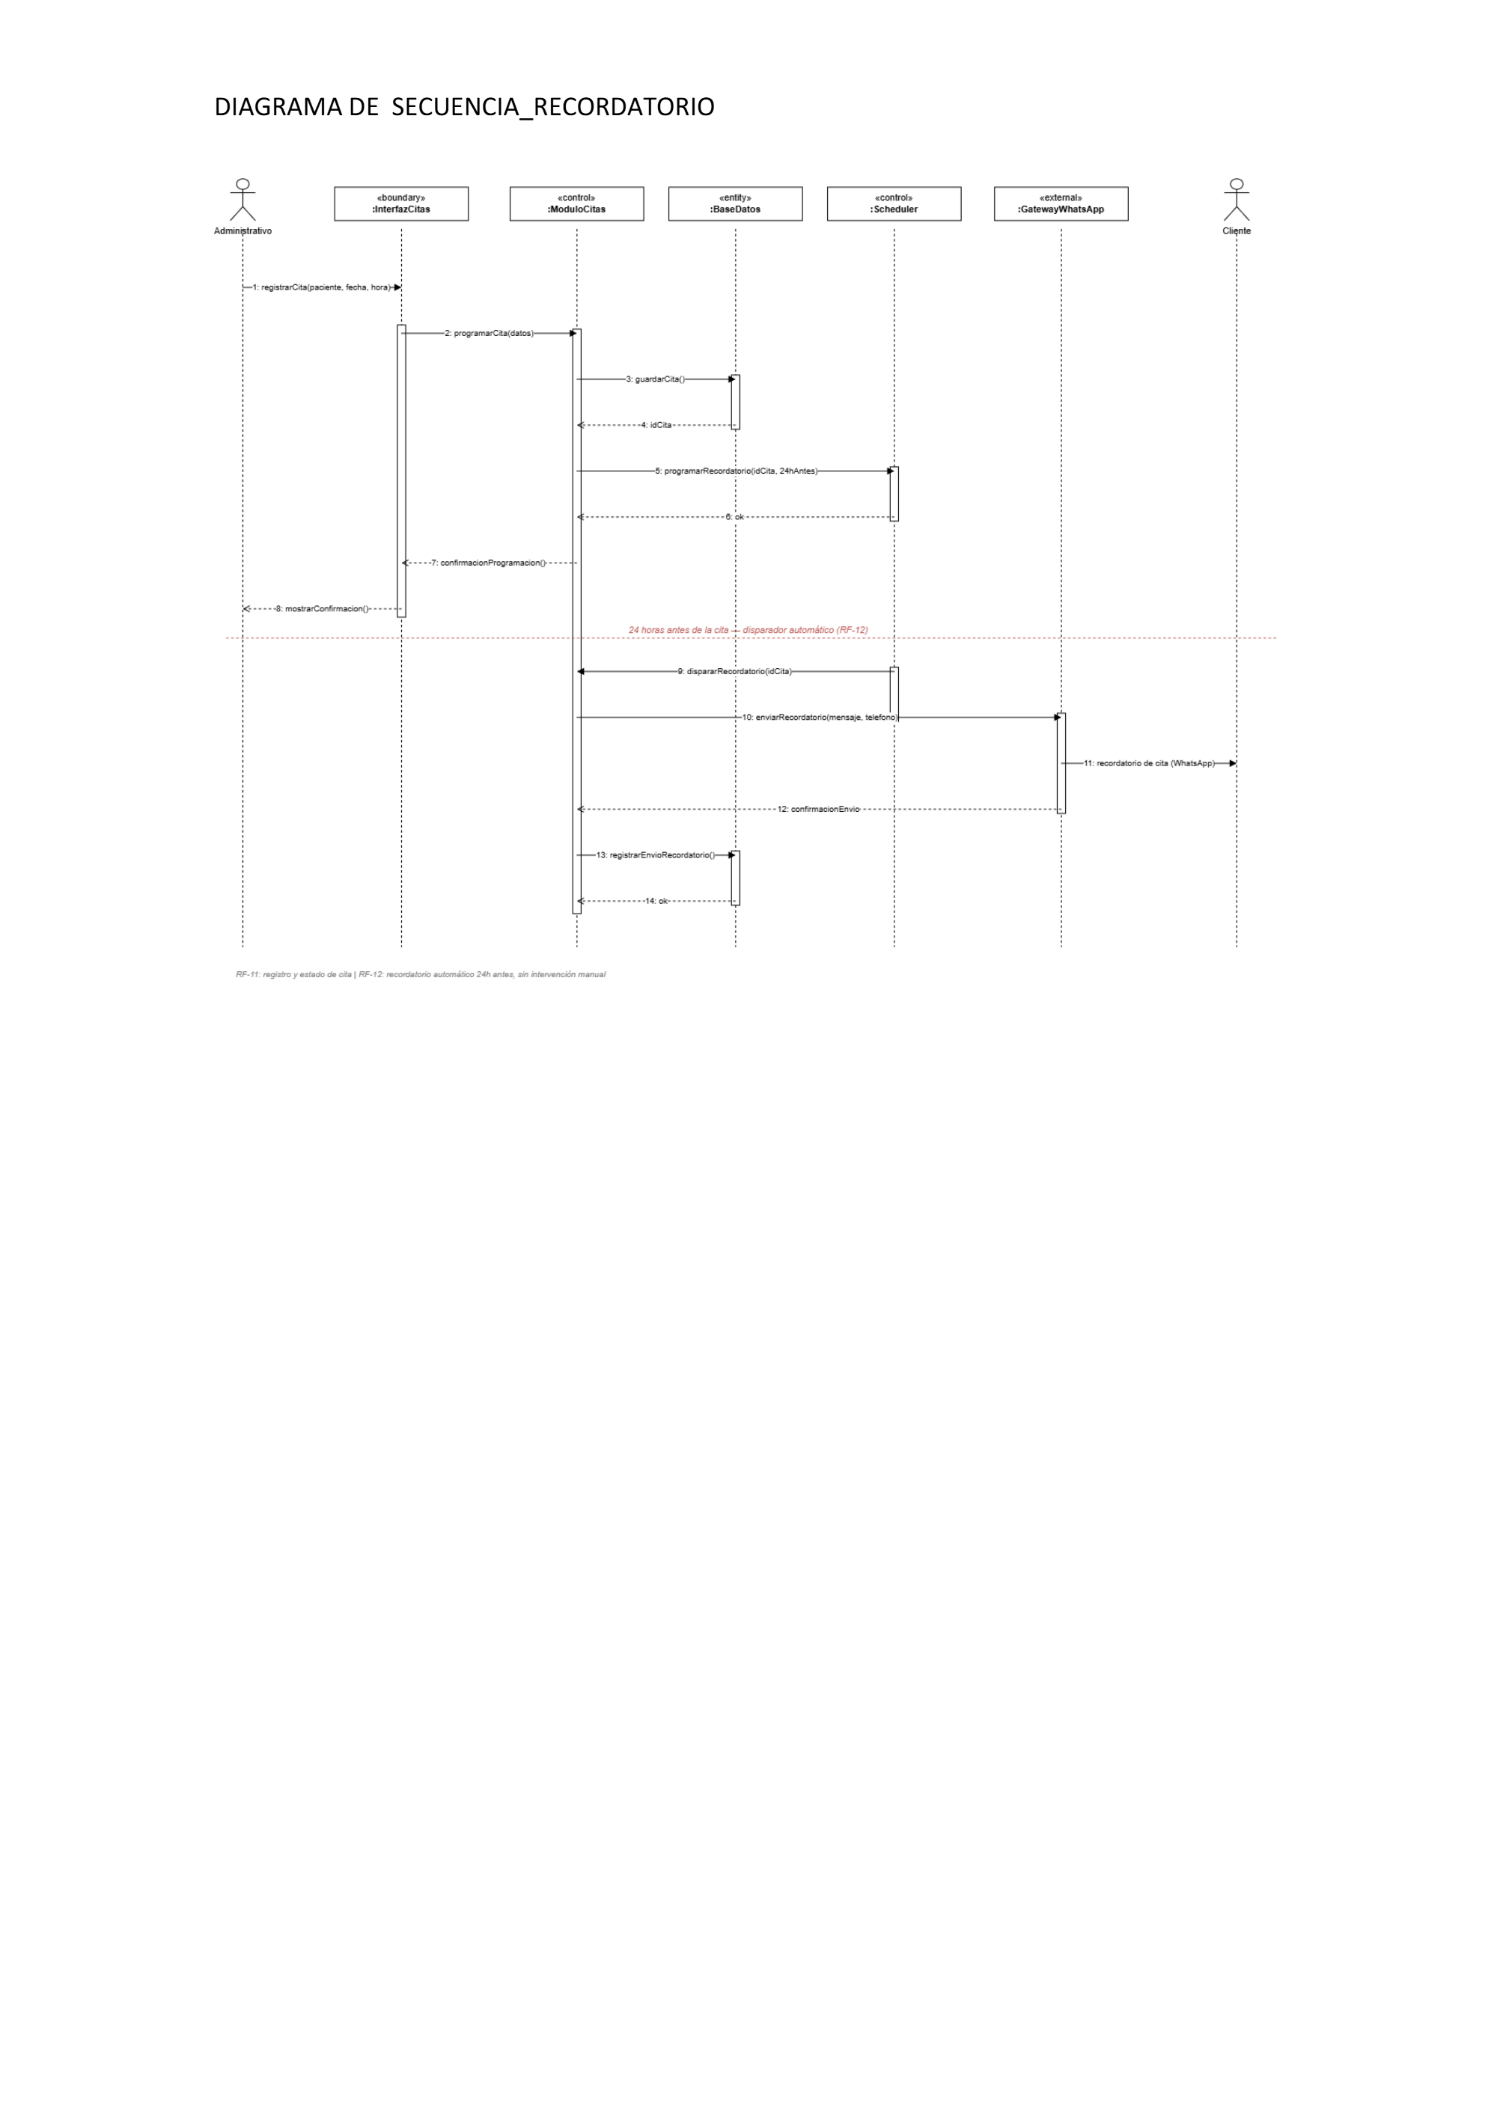
\includegraphics[width=6.79514in,height=4.86905in]{./media/image31.png}

\paragraph{Priorización y
Trazabilidad}\label{priorizaciuxf3n-y-trazabilidad}

\begin{quote}
Clasificar todos los requisitos (RF/NFR/restricción), priorizarlos con
\textbf{MoSCoW} (justificando Must y Won\textquotesingle t) y construir
la \textbf{matriz de trazabilidad parcial} que enlace evidencia de campo
→ requisito → caso de uso.
\end{quote}

\begin{enumerate}
\def\labelenumi{\arabic{enumi}.}
\item
  \protect\phantomsection\label{_bookmark59}{}\textbf{Clasificación de
  Requisitos}
\end{enumerate}

\paragraph{Clasificación de
requisitos}\label{clasificaciuxf3n-de-requisitos}

\paragraph{}\label{section-10}

\begin{quote}
Se clasifican los tres tipos de artefactos de requisitos identificados
en el documento: 24 Requisitos Funcionales (RF), 10 Requisitos No
Funcionales (RNF) y 6 Restricciones (RST), para un total de 40 elementos
clasificados.
\end{quote}

{\def\LTcaptype{none} % do not increment counter
\begin{longtable}[]{@{}
  >{\centering\arraybackslash}p{(\linewidth - 4\tabcolsep) * \real{0.3604}}
  >{\centering\arraybackslash}p{(\linewidth - 4\tabcolsep) * \real{0.2775}}
  >{\centering\arraybackslash}p{(\linewidth - 4\tabcolsep) * \real{0.3184}}@{}}
\toprule\noalign{}
\begin{minipage}[b]{\linewidth}\centering
\textbf{Tipo}
\end{minipage} & \begin{minipage}[b]{\linewidth}\centering
\textbf{Cantidad}
\end{minipage} & \begin{minipage}[b]{\linewidth}\centering
\textbf{Rango de IDs}
\end{minipage} \\
\midrule\noalign{}
\endhead
\bottomrule\noalign{}
\endlastfoot
Requisito Funcional (RF) & 24 & RF-01 a RF-24 \\
Requisito No Funcional (RNF) & 10 & RNF-01 a RNF-10 \\
Restricción (RST) & 6 & RST-01 a RST-06 \\
\end{longtable}
}

\begin{quote}
\protect\phantomsection\label{_bookmark61}{}Tabla 12. Clasificación de
requisitos.
\end{quote}

{\def\LTcaptype{none} % do not increment counter
\begin{longtable}[]{@{}
  >{\raggedright\arraybackslash}p{(\linewidth - 4\tabcolsep) * \real{0.1157}}
  >{\raggedright\arraybackslash}p{(\linewidth - 4\tabcolsep) * \real{0.6334}}
  >{\raggedright\arraybackslash}p{(\linewidth - 4\tabcolsep) * \real{0.2070}}@{}}
\toprule\noalign{}
\begin{minipage}[b]{\linewidth}\centering
\textbf{ID}
\end{minipage} & \begin{minipage}[b]{\linewidth}\centering
\textbf{Restricción}
\end{minipage} & \begin{minipage}[b]{\linewidth}\raggedright
\begin{quote}
\textbf{Origen}
\end{quote}
\end{minipage} \\
\midrule\noalign{}
\endhead
\bottomrule\noalign{}
\endlastfoot
RST-01 & \begin{minipage}[t]{\linewidth}\raggedright
\begin{quote}
Base de datos relacional (PostgreSQL/MySQL), sin NoSQL como
almacenamiento principal.
\end{quote}
\end{minipage} & \begin{minipage}[t]{\linewidth}\raggedright
\begin{quote}
Sección 2.5 / 3.4
\end{quote}
\end{minipage} \\
RST-02 & \begin{minipage}[t]{\linewidth}\raggedright
\begin{quote}
Cumplimiento de la normativa ecuatoriana de protección de datos
personales (LOPDP).
\end{quote}
\end{minipage} & \begin{minipage}[t]{\linewidth}\raggedright
\begin{quote}
Sección 2.6
\end{quote}
\end{minipage} \\
RST-03 & \begin{minipage}[t]{\linewidth}\raggedright
\begin{quote}
Autenticación y RBAC obligatorios por confidencialidad de datos
clínicos.
\end{quote}
\end{minipage} & \begin{minipage}[t]{\linewidth}\raggedright
\begin{quote}
Sección 2.6
\end{quote}
\end{minipage} \\
RST-04 & \begin{minipage}[t]{\linewidth}\raggedright
\begin{quote}
Uso prioritario de frameworks y bibliotecas de código abierto
(presupuesto).
\end{quote}
\end{minipage} & \begin{minipage}[t]{\linewidth}\raggedright
\begin{quote}
Sección 2.6
\end{quote}
\end{minipage} \\
RST-05 & \begin{minipage}[t]{\linewidth}\raggedright
\begin{quote}
Arquitectura cliente-servidor con API REST; módulo de IA desacoplado del
backend.
\end{quote}
\end{minipage} & \begin{minipage}[t]{\linewidth}\raggedright
\begin{quote}
Sección 3.4
\end{quote}
\end{minipage} \\
RST-06 & \begin{minipage}[t]{\linewidth}\raggedright
\begin{quote}
Sincronización offline mediante cola local de operaciones (no réplica
completa de base de datos en cliente).
\end{quote}
\end{minipage} & \begin{minipage}[t]{\linewidth}\raggedright
\begin{quote}
Sección 3.4
\end{quote}
\end{minipage} \\
\end{longtable}
}

\begin{quote}
\protect\phantomsection\label{_bookmark62}{}Tabla 13. Restricciones
clasificadas.
\end{quote}

\subparagraph{Priorización MoSCoW}\label{priorizaciuxf3n-moscow}

{\def\LTcaptype{none} % do not increment counter
\begin{longtable}[]{@{}
  >{\centering\arraybackslash}p{(\linewidth - 6\tabcolsep) * \real{0.1452}}
  >{\raggedright\arraybackslash}p{(\linewidth - 6\tabcolsep) * \real{0.2013}}
  >{\raggedright\arraybackslash}p{(\linewidth - 6\tabcolsep) * \real{0.1875}}
  >{\raggedright\arraybackslash}p{(\linewidth - 6\tabcolsep) * \real{0.4232}}@{}}
\toprule\noalign{}
\begin{minipage}[b]{\linewidth}\centering
\textbf{Prioridad}
\end{minipage} & \begin{minipage}[b]{\linewidth}\centering
\textbf{RF}
\end{minipage} & \begin{minipage}[b]{\linewidth}\centering
\textbf{RNF}
\end{minipage} & \begin{minipage}[b]{\linewidth}\centering
\textbf{Justificación de grupo}
\end{minipage} \\
\midrule\noalign{}
\endhead
\bottomrule\noalign{}
\endlastfoot
Must have & RF-01, RF-02,

RF-03, RF-04,

RF-05, RF-06,

RF-07, RF-08,

RF-09, RF-10,

RF-11, RF-12,

RF-13, RF-14,

RF-15, RF-16, RF-17 (17 RF) &
\begin{minipage}[t]{\linewidth}\raggedright
\begin{quote}
RNF-01, RNF-02, RNF-04, RNF-05, RNF-09 (5 RNF)
\end{quote}
\end{minipage} & Son las funciones sin las cuales el sistema no
reemplaza el proceso manual actual: registro de pacientes, historial
clínico, atención médica con diagnóstico asistido por IA, control de
inventario, gestión de empleados, facturación y comunicación. Sin estos,
SGCV-IA no es operable en una clínica veterinaria

real. \\
\textbf{Prioridad} & \textbf{RF} & \textbf{RNF} & \textbf{Justificación
de grupo} \\
Should have & RF-18, RF-19,

RF-20, RF-21,

RF-22, RF-23 (6 RF) & \begin{minipage}[t]{\linewidth}\raggedright
\begin{quote}
RNF-03, RNF-06, RNF-07 (3 RNF)
\end{quote}
\end{minipage} & Aportan valor significativo (reportes comparativos,
seguimiento nutricional detallado, recordatorios automáticos,
trazabilidad de auditoría) pero el sistema es funcional sin ellos en una
primera versión; pueden incorporarse en una

segunda iteración sin bloquear la operación diaria. \\
\textbf{Prioridad} & \textbf{RF} & \textbf{RNF} & \textbf{Justificación
de grupo} \\
Could have & RF-24 (1 RF) & \begin{minipage}[t]{\linewidth}\raggedright
\begin{quote}
RNF-08, RNF-10 (2 RNF)
\end{quote}
\end{minipage} & La predicción de momento óptimo de cosecha (RF-24)
depende de datos históricos que la clínica todavía no posee (mínimo 2
ciclos de pacientes); la portabilidad extendida (RNF-08) y la \\
\end{longtable}
}

{\def\LTcaptype{none} % do not increment counter
\begin{longtable}[]{@{}
  >{\raggedleft\arraybackslash}p{(\linewidth - 6\tabcolsep) * \real{0.1452}}
  >{\centering\arraybackslash}p{(\linewidth - 6\tabcolsep) * \real{0.2013}}
  >{\centering\arraybackslash}p{(\linewidth - 6\tabcolsep) * \real{0.1875}}
  >{\raggedright\arraybackslash}p{(\linewidth - 6\tabcolsep) * \real{0.4232}}@{}}
\toprule\noalign{}
\begin{minipage}[b]{\linewidth}\raggedleft
\end{minipage} & \begin{minipage}[b]{\linewidth}\centering
\end{minipage} & \begin{minipage}[b]{\linewidth}\centering
\end{minipage} & \begin{minipage}[b]{\linewidth}\raggedright
tolerancia a fallos del proveedor IA (RNF-10) son deseables pero no
garantizables en este alcance.
\end{minipage} \\
\midrule\noalign{}
\endhead
\bottomrule\noalign{}
\endlastfoot
\textbf{Prioridad} & \textbf{RF} & \textbf{RNF} &
\begin{minipage}[t]{\linewidth}\raggedright
\begin{quote}
\textbf{Justificación de grupo}
\end{quote}
\end{minipage} \\
Won\textquotesingle t have & --- &
\begin{minipage}[t]{\linewidth}\centering
\begin{quote}
---
\end{quote}
\end{minipage} & No se identificaron requisitos a excluir explícitamente
del alcance funcional ya definido, dado que las exclusiones de alcance
(diagnósticos definitivos sin validación humana, prescripción
automatizada de medicamentos, integración con sistemas gubernamentales
de salud animal, facturación electrónica certificada ante el SRI,
e-commerce --- Sección 1.2) ya se filtraron en la fase de planificación
(1A) y nunca entraron como RC/RF

candidatos. \\
\end{longtable}
}

\begin{quote}
\protect\phantomsection\label{_bookmark64}{}Tabla 14. Priorización de
requisitos mediante la técnica MoSCoW.

\textbf{Resumen cuantitativo:} 17 Must (71\%), 6 Should (25\%), 1 Could
(4\%), 0 Won\textquotesingle t --- consistente con la regla general de
MoSCoW de no exceder \textasciitilde60\% en Must have. Ajustado al
contexto académico del proyecto.
\end{quote}

\subparagraph{Matriz de Trazabilidad}\label{matriz-de-trazabilidad}

\begin{quote}
Trazabilidad evidencia de campo → requisito → caso de uso. Las
evidencias EV-01 a EV-04 corresponden al registro de evidencias del
Apéndice B (EV-01: entrevista a Dr. Antonio, 24/05/2026; EV-02:
entrevista a Amagua, 25/05/2026; EV-03: acta de reunión firmada; EV-04:
consentimiento informado firmado). Cuando un requisito no corresponde a
uno de los 4 CU detallados en 4.2, se referencia el caso de uso
equivalente del diagrama general (4.1).
\end{quote}

{\def\LTcaptype{none} % do not increment counter
\begin{longtable}[]{@{}
  >{\raggedright\arraybackslash}p{(\linewidth - 14\tabcolsep) * \real{0.0886}}
  >{\raggedright\arraybackslash}p{(\linewidth - 14\tabcolsep) * \real{0.0786}}
  >{\raggedright\arraybackslash}p{(\linewidth - 14\tabcolsep) * \real{0.1258}}
  >{\raggedright\arraybackslash}p{(\linewidth - 14\tabcolsep) * \real{0.1380}}
  >{\raggedright\arraybackslash}p{(\linewidth - 14\tabcolsep) * \real{0.1054}}
  >{\raggedright\arraybackslash}p{(\linewidth - 14\tabcolsep) * \real{0.1506}}
  >{\raggedright\arraybackslash}p{(\linewidth - 14\tabcolsep) * \real{0.1367}}
  >{\raggedright\arraybackslash}p{(\linewidth - 14\tabcolsep) * \real{0.1764}}@{}}
\toprule\noalign{}
\begin{minipage}[b]{\linewidth}\raggedright
\textbf{ID}
\end{minipage} & \begin{minipage}[b]{\linewidth}\raggedright
\textbf{Tipo}
\end{minipage} & \begin{minipage}[b]{\linewidth}\raggedright
\textbf{MoSCoW}
\end{minipage} & \begin{minipage}[b]{\linewidth}\raggedright
\textbf{Kano}
\end{minipage} & \begin{minipage}[b]{\linewidth}\raggedright
\textbf{Valor\\
Negocio}\strut
\end{minipage} & \begin{minipage}[b]{\linewidth}\raggedright
\textbf{Norma/Ley}
\end{minipage} & \begin{minipage}[b]{\linewidth}\raggedright
\textbf{Caso de\\
Uso}\strut
\end{minipage} & \begin{minipage}[b]{\linewidth}\raggedright
\textbf{Mockup /\\
Pantalla}\strut
\end{minipage} \\
\midrule\noalign{}
\endhead
\bottomrule\noalign{}
\endlastfoot
RF-01 & RF & Must & Desempeño & Alto & IEEE 29148 & CU-01 &
\begin{minipage}[t]{\linewidth}\raggedright
Todas las pantallas\\
(responsive)\strut
\end{minipage} \\
RF-02 & RF & Must & Básico & Alto & --- & CU-02 &
\begin{minipage}[t]{\linewidth}\raggedright
Gestión de\\
Historiales Clínicos\strut
\end{minipage} \\
RF-03 & RF & Must & Desempeño & Alto & --- & CU-03 &
\begin{minipage}[t]{\linewidth}\raggedright
Gestión de\\
Historiales Clínicos\strut
\end{minipage} \\
RF-04 & RF & Must & Básico & Alto & LOPDP Art. 4 & CU-02 &
\begin{minipage}[t]{\linewidth}\raggedright
Registro de\\
Consulta\strut
\end{minipage} \\
RF-05 & RF & Must & Desempeño & Alto & --- & CU-04 &
\begin{minipage}[t]{\linewidth}\raggedright
Inventario de\\
Bodega\strut
\end{minipage} \\
RF-06 & RF & Must & Desempeño & Medio & --- & CU-04 &
\begin{minipage}[t]{\linewidth}\raggedright
Inventario de\\
Bodega\strut
\end{minipage} \\
RF-07 & RF & Must & Básico & Alto & --- & CU-02 &
\begin{minipage}[t]{\linewidth}\raggedright
Facturación y\\
Cobro\strut
\end{minipage} \\
RF-08 & RF & Must & Atractivo & Alto & --- & CU-02 &
\begin{minipage}[t]{\linewidth}\raggedright
Facturación y\\
Cobro\strut
\end{minipage} \\
RF-09 & RF & Must & Básico & Medio & LOPDP Art. 4 & CU-02 &
\begin{minipage}[t]{\linewidth}\raggedright
Comunicación\\
con Dueños\strut
\end{minipage} \\
RF-10 & RF & Must & Atractivo & Medio & LOPDP Art. 4 & CU-02 &
\begin{minipage}[t]{\linewidth}\raggedright
Comunicación\\
con Dueños\strut
\end{minipage} \\
RF-11 & RF & Must & Básico & Alto & --- & CU-02 &
\begin{minipage}[t]{\linewidth}\raggedright
Gestión de Citas\\
y Recordatorios\strut
\end{minipage} \\
RF-12 & RF & Should & Atractivo & Medio & --- & CU-02 &
\begin{minipage}[t]{\linewidth}\raggedright
Gestión de Citas\\
y Recordatorios\strut
\end{minipage} \\
RF-13 & RF & Must & Desempeño & Alto & --- & CU-02 &
\begin{minipage}[t]{\linewidth}\raggedright
Seguimiento\\
Nutricional\strut
\end{minipage} \\
RF-14 & RF & Should & Atractivo & Medio & --- & CU-02 &
\begin{minipage}[t]{\linewidth}\raggedright
Seguimiento\\
Nutricional\strut
\end{minipage} \\
RF-15 & RF & Should & Atractivo & Medio & --- & CU-02 &
\begin{minipage}[t]{\linewidth}\raggedright
Gestión de Citas\\
y Recordatorios\strut
\end{minipage} \\
RF-16 & RF & Should & Desempeño & Medio & --- & CU-03 &
\begin{minipage}[t]{\linewidth}\raggedright
Reportes y\\
Exportación\strut
\end{minipage} \\
RF-17 & RF & Must & Atractivo & Alto &
\begin{minipage}[t]{\linewidth}\raggedright
RST-05\\
(ética IA)\strut
\end{minipage} & CU-02 & \begin{minipage}[t]{\linewidth}\raggedright
Panel de\\
Diagnóstico IA\strut
\end{minipage} \\
RF-18 & RF & Should & Básico & Alto & --- & CU-02 &
\begin{minipage}[t]{\linewidth}\raggedright
Panel de\\
Diagnóstico IA\strut
\end{minipage} \\
RF-19 & RF & Should & Básico & Alto & --- & CU-02 &
\begin{minipage}[t]{\linewidth}\raggedright
Panel de\\
Diagnóstico IA\strut
\end{minipage} \\
RF-20 & RF & Should & Básico & Alto & --- & CU-01 &
\begin{minipage}[t]{\linewidth}\raggedright
Login /\\
Selección de rol\strut
\end{minipage} \\
RF-21 & RF & Should & Desempeño & Medio & --- & CU-02 & Dashboard
general* \\
RF-22 & RF & Should & Básico & Alto & --- & CU-01 &
\begin{minipage}[t]{\linewidth}\raggedright
No aplica\\
(criterio de negocio\\
transversal)\strut
\end{minipage} \\
RF-23 & RF & Should & Básico & Alto & LOPDP Art. 4 & CU-01 &
\begin{minipage}[t]{\linewidth}\raggedright
Gestión de Usuarios\\
y Accesos\strut
\end{minipage} \\
RF-24 & RF & Could & Desempeño & Medio &
\begin{minipage}[t]{\linewidth}\raggedright
LOPDP Art. 4\\
(auditoría)\strut
\end{minipage} & CU-03 & \begin{minipage}[t]{\linewidth}\raggedright
Gestión de\\
Historiales Clínicos*\strut
\end{minipage} \\
RNF-01 & RNF & Must & Desempeño & Alto & ISO/IEC 25010 & Transversal &
Transversal \\
RNF-02 & RNF & Must & Desempeño & Alto & ISO/IEC 25010 & CU-02 &
\begin{minipage}[t]{\linewidth}\raggedright
Facturación y\\
Cobro\strut
\end{minipage} \\
RNF-03 & RNF & Should & Desempeño & Medio & ISO/IEC 25010 & CU-04 &
\begin{minipage}[t]{\linewidth}\raggedright
Inventario de\\
Bodega\strut
\end{minipage} \\
RNF-04 & RNF & Must & Básico & Medio & ISO/IEC 25010 & CU-02 & Dashboard
general* \\
RNF-05 & RNF & Must & Básico & Alto &
\begin{minipage}[t]{\linewidth}\raggedright
LOPDP Art. 4 +\\
ISO/IEC 25010\strut
\end{minipage} & CU-01 & \begin{minipage}[t]{\linewidth}\raggedright
Login / Gestión\\
de Usuarios\strut
\end{minipage} \\
RNF-06 & RNF & Should & Básico & Medio & LOPDP Art. 4 & CU-03 &
\begin{minipage}[t]{\linewidth}\raggedright
Gestión de\\
Historiales Clínicos*\strut
\end{minipage} \\
RNF-07 & RNF & Should & Básico & Alto & ISO/IEC 25010 & CU-01 &
\begin{minipage}[t]{\linewidth}\raggedright
Login /\\
Selección de rol\strut
\end{minipage} \\
RNF-08 & RNF & Must & Indiferente & Bajo & ISO/IEC 25010 & CU-01 &
\begin{minipage}[t]{\linewidth}\raggedright
Todas las\\
pantallas\strut
\end{minipage} \\
RNF-09 & RNF & Must & Atractivo & Alto & ISO/IEC 25010 & CU-02 &
\begin{minipage}[t]{\linewidth}\raggedright
Panel de\\
Diagnóstico IA\strut
\end{minipage} \\
RNF-10 & RNF & Could & Indiferente & Bajo & ISO/IEC 25010 & --- &
\begin{minipage}[t]{\linewidth}\raggedright
No aplica\\
(arquitectura interna)\strut
\end{minipage} \\
RST-01 & RST & N/A & N/A & Alto & --- & --- & No aplica \\
RST-02 & RST & N/A & N/A & Alto & LOPDP & CU-01 / CU-03 & No aplica \\
RST-03 & RST & N/A & N/A & Alto & LOPDP Art. 4 & CU-01 & No aplica \\
RST-04 & RST & N/A & N/A & Medio & --- & --- & No aplica \\
RST-05 & RST & N/A & N/A & Alto & --- & CU-02 &
\begin{minipage}[t]{\linewidth}\raggedright
Panel de\\
Diagnóstico IA\strut
\end{minipage} \\
RST-06 & RST & N/A & N/A & Medio & --- & CU-02 &
\begin{minipage}[t]{\linewidth}\raggedright
No aplica\\
(módulo interno)\strut
\end{minipage} \\
\end{longtable}
}

{\def\LTcaptype{none} % do not increment counter
\begin{longtable}[]{@{}
  >{\raggedright\arraybackslash}p{(\linewidth - 4\tabcolsep) * \real{0.1878}}
  >{\raggedright\arraybackslash}p{(\linewidth - 4\tabcolsep) * \real{0.4182}}
  >{\raggedright\arraybackslash}p{(\linewidth - 4\tabcolsep) * \real{0.3503}}@{}}
\toprule\noalign{}
\begin{minipage}[b]{\linewidth}\raggedright
EV-01
\end{minipage} & \begin{minipage}[b]{\linewidth}\raggedright
\begin{quote}
RF-09 --- Registro de comunicaciones post-consulta
\end{quote}
\end{minipage} & \begin{minipage}[b]{\linewidth}\raggedright
CU-02 Registrar Atención Clínica
\end{minipage} \\
\midrule\noalign{}
\endhead
\bottomrule\noalign{}
\endlastfoot
EV-02 & \begin{minipage}[t]{\linewidth}\raggedright
\begin{quote}
RF-10 --- Envío de resultados por WhatsApp
\end{quote}
\end{minipage} & CU-02 Registrar Atención Clínica \\
EV-01, EV-02 & \begin{minipage}[t]{\linewidth}\raggedright
\begin{quote}
RF-11 --- Registro de citas e inasistencias
\end{quote}
\end{minipage} & CU-02 Registrar Atención Clínica \\
EV-02 & \begin{minipage}[t]{\linewidth}\raggedright
\begin{quote}
RF-12 --- Recordatorios automáticos de citas
\end{quote}
\end{minipage} & CU-02 Registrar Atención Clínica \\
EV-01 & \begin{minipage}[t]{\linewidth}\raggedright
\begin{quote}
RF-13 --- Registro de parámetros de crecimiento y peso
\end{quote}
\end{minipage} & CU-02 Registrar Atención Clínica \\
EV-01 & \begin{minipage}[t]{\linewidth}\raggedright
\begin{quote}
RF-14 --- Generación de recomendaciones nutricionales personalizadas
\end{quote}
\end{minipage} & CU-02 Registrar Atención Clínica \\
EV-02 & \begin{minipage}[t]{\linewidth}\raggedright
\begin{quote}
RF-15 --- Programación de recordatorios de seguimiento médico
\end{quote}
\end{minipage} & CU-02 Registrar Atención Clínica \\
EV-01 & \begin{minipage}[t]{\linewidth}\raggedright
\begin{quote}
RF-16 --- Exportación de reportes de salud del paciente
\end{quote}
\end{minipage} & CU-03 Historial Clínico \\
EV-01, EV-02 & \begin{minipage}[t]{\linewidth}\raggedright
\begin{quote}
RF-17 --- Sugerencias diagnósticas basadas en datos clínicos (con
validación obligatoria)
\end{quote}
\end{minipage} & CU-02 Registrar Atención Clínica \\
EV-01, EV-02 & \begin{minipage}[t]{\linewidth}\raggedright
\begin{quote}
RF-18 --- Respaldo de recomendaciones en literatura científica
veterinaria validada
\end{quote}
\end{minipage} & CU-02 Registrar Atención Clínica \\
EV-01, EV-02 & \begin{minipage}[t]{\linewidth}\raggedright
\begin{quote}
RF-19 --- Capacidad de revisión y corrección de sugerencias de IA por
parte del veterinario
\end{quote}
\end{minipage} & CU-02 Registrar Atención Clínica \\
EV-01, EV-02 & \begin{minipage}[t]{\linewidth}\raggedright
\begin{quote}
RF-20 --- Interfaz sencilla sin capacitación prolongada
\end{quote}
\end{minipage} & CU-01 Iniciar Sesión \\
EV-01, EV-02 & \begin{minipage}[t]{\linewidth}\raggedright
\begin{quote}
RF-21 --- Operación con baja dependencia de conectividad permanente
\end{quote}
\end{minipage} & CU-02 Registrar Atención Clínica \\
EV-01 & \begin{minipage}[t]{\linewidth}\raggedright
\begin{quote}
RF-22 --- Bajo costo de implementación y operación
\end{quote}
\end{minipage} & CU-01 Iniciar Sesión \\
EV-01, EV-02 & \begin{minipage}[t]{\linewidth}\raggedright
\begin{quote}
RF-23 --- Perfiles de usuario diferenciados con control de acceso
\end{quote}
\end{minipage} & CU-01 Iniciar Sesión \\
EV-02 & \begin{minipage}[t]{\linewidth}\raggedright
\begin{quote}
RF-24 --- Trazabilidad de cambios en historiales clínicos
\end{quote}
\end{minipage} & CU-03 Historial Clínico \\
\end{longtable}
}

\protect\phantomsection\label{_bookmark66}{}\emph{\textbf{Tabla 15
Matriz de trazabilidad}}

\paragraph{Conclusiones}\label{conclusiones}

\begin{quote}
La Entrega 1B consolidó en un único documento la planificación y la
elicitación de la Entrega 1A (ajustada según la retroalimentación
docente) junto con la especificación parcial del sistema SGCV-IA. Se
clasificaron 40 elementos de requisitos: 24 requisitos funcionales
(RF-01 a RF-24), 10 requisitos no funcionales cuantificados según
ISO/IEC 25010 y 6 restricciones de diseño, todos trazados a la evidencia
de campo recolectada durante la elicitación.

Se construyó el modelado UML inicial: un diagrama de casos de uso
general, la especificación textual detallada de cinco casos de uso
(CU-01 a CU-05, entre ellos Iniciar Sesión, Registrar Atención Clínica,
Revisar Historial Clínico, Controlar Inventario y Gestionar Empleados) y
un diagrama de clases conceptual con diez relaciones principales
debidamente justificadas y con su multiplicidad definida entre las
entidades del dominio (Usuario, Paciente, Historial Clínico, Atención
Clínica, Inventario, entre otras).

Entre las decisiones de diseño tempranas destacan la arquitectura
cliente-servidor con API REST y módulo de IA desacoplado del backend, el
almacenamiento en base de datos relacional MySQL, la sincronización
offline mediante cola local de operaciones y el asistente de diagnóstico
basado en inteligencia artificial, cuyas sugerencias requieren
validación obligatoria del veterinario y respaldo en literatura
científica. El alcance se acotó de forma explícita, excluyendo
diagnósticos definitivos sin supervisión humana, la prescripción
automática de medicamentos, la integración con sistemas gubernamentales
de salud animal y la facturación electrónica certificada ante el SRI.

La trazabilidad quedó establecida de extremo a extremo (evidencia →
requisito → caso de uso) en una matriz con cobertura del 100\% sobre los
24 requisitos funcionales, sustentada en dos entrevistas
semiestructuradas a médicos veterinarios (Veterinaria Colombia y
Veterinaria Macay) con consentimiento informado firmado, complementadas
con observación directa de los procesos clínicos y administrativos. La
priorización MoSCoW resultó en 17 requisitos Must have, 6 Should have y
1 Could have, sin elementos Won\textquotesingle t have, ya que las
exclusiones de alcance se habían delimitado desde la fase de
planificación.

Como trabajo pendiente para la siguiente entrega se contempla: maquetar
los mockups de las pantallas principales en Figma y enlazarlos
formalmente a los requisitos, refinar los requisitos más volátiles (en
especial los asociados al módulo de inteligencia artificial), elaborar
el diseño detallado de la arquitectura del sistema, y validar nuevamente
la especificación con los stakeholders entrevistados.
\end{quote}

\subsection{APÉNDICE A --- PLAN DEL PROYECTO DE INGENIERÍA DE
REQUISITOS}\label{apuxe9ndice-a-plan-del-proyecto-de-ingenieruxeda-de-requisitos}

\subsubsection{Identificación y Análisis de
Stakeholders}\label{identificaciuxf3n-y-anuxe1lisis-de-stakeholders}

\begin{quote}
Se identificaron los siguientes stakeholders a partir del contexto del
dominio y las entrevistas realizadas:
\end{quote}

{\def\LTcaptype{none} % do not increment counter
\begin{longtable}[]{@{}
  >{\raggedright\arraybackslash}p{(\linewidth - 8\tabcolsep) * \real{0.2668}}
  >{\raggedright\arraybackslash}p{(\linewidth - 8\tabcolsep) * \real{0.1747}}
  >{\centering\arraybackslash}p{(\linewidth - 8\tabcolsep) * \real{0.1333}}
  >{\centering\arraybackslash}p{(\linewidth - 8\tabcolsep) * \real{0.1131}}
  >{\raggedright\arraybackslash}p{(\linewidth - 8\tabcolsep) * \real{0.2730}}@{}}
\toprule\noalign{}
\begin{minipage}[b]{\linewidth}\raggedright
\begin{quote}
\textbf{Nombre / Rol}
\end{quote}
\end{minipage} & \begin{minipage}[b]{\linewidth}\centering
\textbf{Tipo}
\end{minipage} & \begin{minipage}[b]{\linewidth}\centering
\textbf{Influencia}
\end{minipage} & \begin{minipage}[b]{\linewidth}\centering
\textbf{Interés}
\end{minipage} & \begin{minipage}[b]{\linewidth}\raggedright
\begin{quote}
\textbf{Necesidades y expectativas}
\end{quote}
\end{minipage} \\
\midrule\noalign{}
\endhead
\bottomrule\noalign{}
\endlastfoot
\textbf{Dr. Antonio --- Médico Veterinario (Entrevistado 1)} &
\begin{minipage}[t]{\linewidth}\raggedright
\begin{quote}
Usuario primario
\end{quote}
\end{minipage} & Alta & Alta & Base de datos contable, acceso móvil,
bajo costo, facilidad de uso, soporte diagnóstico moderado. \\
\textbf{Amagua --- Médico Veterinario / Personal Clínico (Entrevistado
2)} & \begin{minipage}[t]{\linewidth}\raggedright
\begin{quote}
Usuario primario
\end{quote}
\end{minipage} & Alta & Alta & Facturación ágil, control de
vencimientos, historial organizado por nombre/dueño, portabilidad

(móvil + PC). \\
\textbf{Personal Administrativo --- clínica} &
\begin{minipage}[t]{\linewidth}\raggedright
\begin{quote}
Usuario secundario
\end{quote}
\end{minipage} & Media & Alta & Gestión centralizada de BD, control de
inventario y vencimientos. \\
\textbf{Dueños de mascotas} &
\begin{minipage}[t]{\linewidth}\raggedright
\begin{quote}
Usuario externo
\end{quote}
\end{minipage} & Baja & Media & Seguimiento post-consulta, recordatorios
de citas, resultados de exámenes por

WhatsApp. \\
\textbf{Equipo de desarrollo SGCV-IA} &
\begin{minipage}[t]{\linewidth}\raggedright
\begin{quote}
Parte interesada interna
\end{quote}
\end{minipage} & Alta & Alta & Requisitos claros, trazables y
verificables para implementar el sistema. \\
\end{longtable}
}

\protect\phantomsection\label{_bookmark70}{}\emph{\textbf{Tabla 16.
Identificación y Análisis de Stakeholders}}

\subparagraph{Cronograma de Actividades de Ingeniería de
Requisitos}\label{cronograma-de-actividades-de-ingenieruxeda-de-requisitos}

{\def\LTcaptype{none} % do not increment counter
\begin{longtable}[]{@{}
  >{\raggedright\arraybackslash}p{(\linewidth - 6\tabcolsep) * \real{0.3280}}
  >{\centering\arraybackslash}p{(\linewidth - 6\tabcolsep) * \real{0.1846}}
  >{\centering\arraybackslash}p{(\linewidth - 6\tabcolsep) * \real{0.1846}}
  >{\raggedright\arraybackslash}p{(\linewidth - 6\tabcolsep) * \real{0.2626}}@{}}
\toprule\noalign{}
\begin{minipage}[b]{\linewidth}\centering
\textbf{Actividad}
\end{minipage} & \begin{minipage}[b]{\linewidth}\centering
\textbf{Fecha inicio}
\end{minipage} & \begin{minipage}[b]{\linewidth}\centering
\textbf{Fecha fin}
\end{minipage} & \begin{minipage}[b]{\linewidth}\raggedright
\begin{quote}
\textbf{Responsable}
\end{quote}
\end{minipage} \\
\midrule\noalign{}
\endhead
\bottomrule\noalign{}
\endlastfoot
Definición del sistema objetivo y selección de stakeholders & 19/05/2026
& 21/05/2026 & \begin{minipage}[t]{\linewidth}\raggedright
\begin{quote}
Analista líder
\end{quote}
\end{minipage} \\
Diseño del instrumento de entrevista (SGCV-IA PreguntasV1) & 21/05/2026
& 23/05/2026 & \begin{minipage}[t]{\linewidth}\raggedright
\begin{quote}
Equipo completo
\end{quote}
\end{minipage} \\
Entrevista semiestructurada --- Dr. Antonio (Entrevistado 1) &
24/05/2026 & 24/05/2026 & \begin{minipage}[t]{\linewidth}\raggedright
\begin{quote}
Marcillo / Vera
\end{quote}
\end{minipage} \\
Entrevista semiestructurada --- Amagua (Entrevistado 2) & 25/05/2026 &
25/05/2026 & \begin{minipage}[t]{\linewidth}\raggedright
\begin{quote}
Barrionuevo / Mesias
\end{quote}
\end{minipage} \\
Transcripción y análisis de entrevistas & 26/05/2026 & 27/05/2026 &
\begin{minipage}[t]{\linewidth}\raggedright
\begin{quote}
Documentador
\end{quote}
\end{minipage} \\
Extracción de requisitos crudos (RC-01 a RC-21) & 27/05/2026 &
28/05/2026 & \begin{minipage}[t]{\linewidth}\raggedright
\begin{quote}
Verificador
\end{quote}
\end{minipage} \\
Redacción del documento ERS v1.0 (Entrega 1A) & 28/05/2026 & 31/05/2026
& \begin{minipage}[t]{\linewidth}\raggedright
\begin{quote}
Equipo completo
\end{quote}
\end{minipage} \\
Entrega 1A al docente & 31/05/2026 & 31/05/2026 &
\begin{minipage}[t]{\linewidth}\raggedright
\begin{quote}
Analista líder
\end{quote}
\end{minipage} \\
Correcciones según retroalimentación del docente & 01/06/2026 &
15/06/2026 & \begin{minipage}[t]{\linewidth}\raggedright
\begin{quote}
Documentador
\end{quote}
\end{minipage} \\
Elaboración de mockups, RF formales, RNF, UML (Entrega 1B) & 15/06/2026
& 12/07/2026 & \begin{minipage}[t]{\linewidth}\raggedright
\begin{quote}
Modelador + Equipo
\end{quote}
\end{minipage} \\
\end{longtable}
}

\protect\phantomsection\label{_bookmark72}{}\emph{\textbf{Tabla 17.
Cronograma de Actividades de Ingeniería de Requisitos}}

\paragraph{Técnicas de Elicitación Seleccionadas y
Justificación}\label{tuxe9cnicas-de-elicitaciuxf3n-seleccionadas-y-justificaciuxf3n}

{\def\LTcaptype{none} % do not increment counter
\begin{longtable}[]{@{}
  >{\raggedright\arraybackslash}p{(\linewidth - 4\tabcolsep) * \real{0.2254}}
  >{\raggedright\arraybackslash}p{(\linewidth - 4\tabcolsep) * \real{0.3850}}
  >{\raggedright\arraybackslash}p{(\linewidth - 4\tabcolsep) * \real{0.3484}}@{}}
\toprule\noalign{}
\begin{minipage}[b]{\linewidth}\centering
\textbf{Técnica}
\end{minipage} & \begin{minipage}[b]{\linewidth}\raggedright
\begin{quote}
\textbf{Descripción aplicada}
\end{quote}
\end{minipage} & \begin{minipage}[b]{\linewidth}\centering
\textbf{Justificación}
\end{minipage} \\
\midrule\noalign{}
\endhead
\bottomrule\noalign{}
\endlastfoot
\textbf{Entrevista semiestructurada} & Se elaboró un instrumento con 20
preguntas distribuidas en cuatro secciones (A: Gestión Operativa, B:
Seguimiento Clínico, C: Percepción de IA, D: Criterios de Adopción). Se
aplicó a dos veterinarios

reales con consentimiento informado. &
\begin{minipage}[t]{\linewidth}\raggedright
\begin{quote}
Permite capturar tanto datos cuantitativos (escalas) como cualitativos
(narrativa libre). Apropiada para dominios con usuarios de experiencia
digital básica que no

sabrían responder una encuesta técnica.
\end{quote}
\end{minipage} \\
\textbf{Análisis de documentos existentes} & Se analizó la descripción
del sistema objetivo (Proyecto\_1\_vcty) para identificar el problema de
dominio y el contexto

organizacional. & \begin{minipage}[t]{\linewidth}\raggedright
\begin{quote}
Permite validar que la elicitación oral coincide con el diagnóstico
previo del equipo, reduciendo contradicciones.
\end{quote}
\end{minipage} \\
\textbf{Observación directa (registro durante la entrevista)} & Durante
las entrevistas se registraron las herramientas actualmente en uso (Buff
Note, programa de facturación en línea,

WhatsApp), sus limitaciones y el flujo de trabajo informal. &
\begin{minipage}[t]{\linewidth}\raggedright
\begin{quote}
Complementa la entrevista con evidencia de comportamiento real, no solo
declarado.
\end{quote}
\end{minipage} \\
\end{longtable}
}

\begin{quote}
\protect\phantomsection\label{_bookmark74}{}\emph{\textbf{Tabla 18.
Técnicas de Elicitación Seleccionadas y Justificación}}
\end{quote}

\subsection{APÉNDICE B --- EVIDENCIAS DE
ELICITACIÓN}\label{apuxe9ndice-b-evidencias-de-elicitaciuxf3n}

\subsubsection{Instrumento de
Entrevista}\label{instrumento-de-entrevista}

{\def\LTcaptype{none} % do not increment counter
\begin{longtable}[]{@{}
  >{\raggedright\arraybackslash}p{(\linewidth - 10\tabcolsep) * \real{0.0611}}
  >{\raggedright\arraybackslash}p{(\linewidth - 10\tabcolsep) * \real{0.1386}}
  >{\centering\arraybackslash}p{(\linewidth - 10\tabcolsep) * \real{0.1160}}
  >{\raggedright\arraybackslash}p{(\linewidth - 10\tabcolsep) * \real{0.2153}}
  >{\raggedright\arraybackslash}p{(\linewidth - 10\tabcolsep) * \real{0.2681}}
  >{\raggedright\arraybackslash}p{(\linewidth - 10\tabcolsep) * \real{0.1603}}@{}}
\toprule\noalign{}
\begin{minipage}[b]{\linewidth}\raggedright
\begin{quote}
\textbf{ID-EV}
\end{quote}
\end{minipage} & \begin{minipage}[b]{\linewidth}\centering
\textbf{Tipo}
\end{minipage} & \begin{minipage}[b]{\linewidth}\centering
\textbf{Fecha}
\end{minipage} & \begin{minipage}[b]{\linewidth}\raggedright
\begin{quote}
\textbf{Fuente / participante (rol)}
\end{quote}
\end{minipage} & \begin{minipage}[b]{\linewidth}\raggedright
\begin{quote}
\textbf{Información obtenida}
\end{quote}
\end{minipage} & \begin{minipage}[b]{\linewidth}\raggedright
\textbf{Consentimiento}
\end{minipage} \\
\midrule\noalign{}
\endhead
\bottomrule\noalign{}
\endlastfoot
\textbf{EV-01} & Entrevista (audio) & 23/05/2026 & Dr. Diego Jaramillo
-- Médico veterinario y

propietario de la Veterinaria Colombia &
\begin{minipage}[t]{\linewidth}\raggedright
\begin{quote}
Información sobre el proceso de atención, registro de

pacientes, inventario y facturación.
\end{quote}
\end{minipage} & Sí \\
\textbf{EV-02} & Entrevista (audio) & 26/05/2026 & Dr. Bryan Macay --
Médico veterinario de la Veterinaria Macay &
\begin{minipage}[t]{\linewidth}\raggedright
\begin{quote}
Información sobre el seguimiento clínico, control de tratamientos y uso
de inteligencia artificial como apoyo al diagnóstico.
\end{quote}
\end{minipage} & Sí \\
\textbf{EV-03} & Observación de campo & 23/05/2026 & Veterinaria
Colombia & \begin{minipage}[t]{\linewidth}\raggedright
\begin{quote}
Observación de los procesos de atención y registro de

información clínica.
\end{quote}
\end{minipage} & N/A \\
\end{longtable}
}

\protect\phantomsection\label{_bookmark77}{}\emph{\textbf{Tabla 19.
Instrumento de Entrevista}}

\subsubsection{Actas de Reunión con
Stakeholders}\label{actas-de-reuniuxf3n-con-stakeholders}

\begin{enumerate}
\def\labelenumi{\arabic{enumi}.}
\item
  \protect\phantomsection\label{_bookmark78}{}\textbf{--- Acta de
  Entrevista N.° 1: Veterinaria Colombia}
\end{enumerate}

{\def\LTcaptype{none} % do not increment counter
\begin{longtable}[]{@{}
  >{\raggedright\arraybackslash}p{(\linewidth - 2\tabcolsep) * \real{0.1794}}
  >{\raggedright\arraybackslash}p{(\linewidth - 2\tabcolsep) * \real{0.7758}}@{}}
\toprule\noalign{}
\begin{minipage}[b]{\linewidth}\centering
\textbf{Dato}
\end{minipage} & \begin{minipage}[b]{\linewidth}\centering
\textbf{Información}
\end{minipage} \\
\midrule\noalign{}
\endhead
\bottomrule\noalign{}
\endlastfoot
\textbf{Stakeholder entrevistado} &
\begin{minipage}[t]{\linewidth}\raggedright
\begin{quote}
Dr. Diego Jaramillo
\end{quote}
\end{minipage} \\
\textbf{Experiencia} & \begin{minipage}[t]{\linewidth}\raggedright
\begin{quote}
8 años como medico veterinario
\end{quote}
\end{minipage} \\
\textbf{Rol en la clínica} & \begin{minipage}[t]{\linewidth}\raggedright
\begin{quote}
Médico veterinario y propietario de un establecimiento dedicado a la
atención clínica y venta de productos veterinarios.
\end{quote}
\end{minipage} \\
\textbf{Entrevistador} & \begin{minipage}[t]{\linewidth}\raggedright
\begin{quote}
Anthony Vera Gómez
\end{quote}
\end{minipage} \\
\textbf{Fecha de la entrevista} &
\begin{minipage}[t]{\linewidth}\raggedright
\begin{quote}
23 de mayo de 2026
\end{quote}
\end{minipage} \\
\textbf{Lugar} & \begin{minipage}[t]{\linewidth}\raggedright
\begin{quote}
Veterinaria Colombia-El empalme
\end{quote}
\end{minipage} \\
\textbf{Modalidad} & \begin{minipage}[t]{\linewidth}\raggedright
\begin{quote}
Presencial, con grabación de audio y consentimiento informado.
\end{quote}
\end{minipage} \\
\textbf{Duración aproximada} &
\begin{minipage}[t]{\linewidth}\raggedright
\begin{quote}
12:

30 minutos
\end{quote}
\end{minipage} \\
\textbf{Técnica de elicitación} &
\begin{minipage}[t]{\linewidth}\raggedright
\begin{quote}
Entrevista semiestructurada.
\end{quote}
\end{minipage} \\
\textbf{Objetivo de la sesión} &
\begin{minipage}[t]{\linewidth}\raggedright
\begin{quote}
Recopilar información sobre los procesos clínicos, administrativos y las
necesidades de la clínica veterinaria para identificar los requisitos
del Sistema de Gestión Clínica Veterinaria con Inteligencia Artificial
(SGCV-IA).
\end{quote}
\end{minipage} \\
\end{longtable}
}

\protect\phantomsection\label{_bookmark79}{}\emph{\textbf{Tabla 20. Acta
de Entrevista N.° 1}}

\begin{quote}
Resumen de hallazgos clave por sección:
\end{quote}

{\def\LTcaptype{none} % do not increment counter
\begin{longtable}[]{@{}
  >{\centering\arraybackslash}p{(\linewidth - 4\tabcolsep) * \real{0.0614}}
  >{\raggedright\arraybackslash}p{(\linewidth - 4\tabcolsep) * \real{0.2561}}
  >{\raggedright\arraybackslash}p{(\linewidth - 4\tabcolsep) * \real{0.6411}}@{}}
\toprule\noalign{}
\begin{minipage}[b]{\linewidth}\centering
\textbf{ID}
\end{minipage} & \begin{minipage}[b]{\linewidth}\centering
\textbf{Pregunta}
\end{minipage} & \begin{minipage}[b]{\linewidth}\raggedright
\begin{quote}
\textbf{Respuesta / Hallazgo relevante}
\end{quote}
\end{minipage} \\
\midrule\noalign{}
\endhead
\bottomrule\noalign{}
\endlastfoot
A1 & \textbf{Obtención de información clínica} &
\begin{minipage}[t]{\linewidth}\raggedright
\begin{quote}
Los propietarios suelen acudir en la etapa terminal del animal; la
información llega tarde y sin historial previo.
\end{quote}
\end{minipage} \\
A2 & \textbf{Dificultades con el historial} &
\begin{minipage}[t]{\linewidth}\raggedright
\begin{quote}
Falta de información de los propietarios sobre enfermedades previas; los
síntomas se presentan en etapas avanzadas.
\end{quote}
\end{minipage} \\
A3 & \textbf{Proceso de cobro y facturación} &
\begin{minipage}[t]{\linewidth}\raggedright
\begin{quote}
No se enfrenta ningún inconveniente: se informa el costo al propietario
antes del tratamiento y se trabaja con efectivo en un entorno de
confianza.
\end{quote}
\end{minipage} \\
A4 & \textbf{Control de inventario} &
\begin{minipage}[t]{\linewidth}\raggedright
\begin{quote}
No existe inventario formal. Los productos veterinarios suelen caducar
por falta de control sistemático.
\end{quote}
\end{minipage} \\
A5 & \textbf{Inasistencias} &
\begin{minipage}[t]{\linewidth}\raggedright
\begin{quote}
No aplica: el negocio opera como punto de venta de productos; no hay
sistema de citas.
\end{quote}
\end{minipage} \\
\end{longtable}
}

{\def\LTcaptype{none} % do not increment counter
\begin{longtable}[]{@{}
  >{\centering\arraybackslash}p{(\linewidth - 4\tabcolsep) * \real{0.0614}}
  >{\raggedright\arraybackslash}p{(\linewidth - 4\tabcolsep) * \real{0.2561}}
  >{\raggedright\arraybackslash}p{(\linewidth - 4\tabcolsep) * \real{0.6411}}@{}}
\toprule\noalign{}
\begin{minipage}[b]{\linewidth}\centering
A6
\end{minipage} & \begin{minipage}[b]{\linewidth}\raggedright
\textbf{Comunicación post-consulta}
\end{minipage} & \begin{minipage}[b]{\linewidth}\raggedright
\begin{quote}
Se realiza por llamadas telefónicas.
\end{quote}
\end{minipage} \\
\midrule\noalign{}
\endhead
\bottomrule\noalign{}
\endlastfoot
B1 & \textbf{Seguimiento nutricional} &
\begin{minipage}[t]{\linewidth}\raggedright
\begin{quote}
Se inculca al dueño una alimentación adecuada según la raza y la etapa
de crecimiento del animal.
\end{quote}
\end{minipage} \\
B2 & \textbf{Consultas sobre alimentación} &
\begin{minipage}[t]{\linewidth}\raggedright
\begin{quote}
Las recomendaciones se basan en la condición corporal del animal durante
la consulta presencial.
\end{quote}
\end{minipage} \\
B3 & \textbf{Cumplimiento de indicaciones} &
\begin{minipage}[t]{\linewidth}\raggedright
\begin{quote}
Se espera cumplimiento riguroso; los controles programados son
esenciales para la recuperación.
\end{quote}
\end{minipage} \\
B4 & \textbf{Ajuste sin ver al animal} &
\begin{minipage}[t]{\linewidth}\raggedright
\begin{quote}
Si el tratamiento no mejora, se refiere a clínicas con mayor
equipamiento o se solicitan pruebas de sangre.
\end{quote}
\end{minipage} \\
C1 & \textbf{Herramientas digitales} &
\begin{minipage}[t]{\linewidth}\raggedright
\begin{quote}
No utiliza ningún software o herramienta digital especializada.
\end{quote}
\end{minipage} \\
C2 & \textbf{Acuerdo con diagnóstico por IA} &
\begin{minipage}[t]{\linewidth}\raggedright
\begin{quote}
Escala: 4/5 (de acuerdo).
\end{quote}
\end{minipage} \\
C3 & \textbf{Mayor carga de trabajo} &
\begin{minipage}[t]{\linewidth}\raggedright
\begin{quote}
No identifica una carga específica.
\end{quote}
\end{minipage} \\
C4 & \textbf{Nivel de confianza en IA} &
\begin{minipage}[t]{\linewidth}\raggedright
\begin{quote}
Confianza moderada: usaría la IA como apoyo con validación propia.
\end{quote}
\end{minipage} \\
C5 & \textbf{Condición más importante para confiar} &
\begin{minipage}[t]{\linewidth}\raggedright
\begin{quote}
Que las recomendaciones sean confiables y estén respaldadas
científicamente para diagnosticar animales.
\end{quote}
\end{minipage} \\
D1 & \textbf{Primer problema a resolver} &
\begin{minipage}[t]{\linewidth}\raggedright
\begin{quote}
Una base de datos contable que ayude a llevar la contabilidad del
negocio.
\end{quote}
\end{minipage} \\
D2 & \textbf{Características indispensables} &
\begin{minipage}[t]{\linewidth}\raggedright
\begin{quote}
Facilidad de uso y bajo valor económico.
\end{quote}
\end{minipage} \\
D3 & \textbf{Dispositivo preferido} &
\begin{minipage}[t]{\linewidth}\raggedright
\begin{quote}
Teléfono móvil.
\end{quote}
\end{minipage} \\
D4 & \textbf{Problemas de conectividad} &
\begin{minipage}[t]{\linewidth}\raggedright
\begin{quote}
Nivel 2-3/5.
\end{quote}
\end{minipage} \\
D5 & \textbf{Necesidades no abordadas} &
\begin{minipage}[t]{\linewidth}\raggedright
\begin{quote}
Todo fue cubierto; reconoce necesidad de adaptarse a la modernización
tecnológica.
\end{quote}
\end{minipage} \\
\end{longtable}
}

\protect\phantomsection\label{_bookmark80}{}\emph{\textbf{Tabla 21. Acta
de Entrevista N.° 1- hallazgos}}

\begin{enumerate}
\def\labelenumi{\arabic{enumi}.}
\setcounter{enumi}{1}
\item
  \textbf{--- Acta de Entrevista N.° 2: Veterinaria Macay}
\end{enumerate}

{\def\LTcaptype{none} % do not increment counter
\begin{longtable}[]{@{}
  >{\raggedright\arraybackslash}p{(\linewidth - 2\tabcolsep) * \real{0.1942}}
  >{\raggedright\arraybackslash}p{(\linewidth - 2\tabcolsep) * \real{0.7610}}@{}}
\toprule\noalign{}
\begin{minipage}[b]{\linewidth}\centering
\textbf{Dato}
\end{minipage} & \begin{minipage}[b]{\linewidth}\centering
\textbf{Información}
\end{minipage} \\
\midrule\noalign{}
\endhead
\bottomrule\noalign{}
\endlastfoot
\textbf{Stakeholder}

\textbf{entrevistado} & \begin{minipage}[t]{\linewidth}\raggedright
\begin{quote}
Dr. Bryan Macay
\end{quote}
\end{minipage} \\
\textbf{Experiencia} & \begin{minipage}[t]{\linewidth}\raggedright
\begin{quote}
3-4 años como médico veterinario
\end{quote}
\end{minipage} \\
\textbf{Rol en la clínica} & \begin{minipage}[t]{\linewidth}\raggedright
\begin{quote}
Médico veterinario con funciones clínicas y de registro.
\end{quote}
\end{minipage} \\
\textbf{Entrevistador} & \begin{minipage}[t]{\linewidth}\raggedright
\begin{quote}
Robyn Amagua Sacon
\end{quote}
\end{minipage} \\
\textbf{Fecha de la}

\textbf{entrevista} & \begin{minipage}[t]{\linewidth}\raggedright
\begin{quote}
26 de mayo de 2026
\end{quote}
\end{minipage} \\
\textbf{Lugar} & \begin{minipage}[t]{\linewidth}\raggedright
\begin{quote}
Veterinaria Macay-El empalme
\end{quote}
\end{minipage} \\
\textbf{Modalidad} & \begin{minipage}[t]{\linewidth}\raggedright
\begin{quote}
Presencial, con grabación de audio y consentimiento informado.
\end{quote}
\end{minipage} \\
\textbf{Duración}

\textbf{aproximada} & \begin{minipage}[t]{\linewidth}\raggedright
\begin{quote}
10 minutos.
\end{quote}
\end{minipage} \\
\textbf{Técnica de}

\textbf{elicitación} & \begin{minipage}[t]{\linewidth}\raggedright
\begin{quote}
Entrevista semiestructurada.
\end{quote}
\end{minipage} \\
\textbf{Objetivo de la}

\textbf{sesión} & \begin{minipage}[t]{\linewidth}\raggedright
\begin{quote}
Identificar las necesidades y requerimientos de la clínica para el
desarrollo del Sistema de

Gestión Clínica Veterinaria con Inteligencia Artificial (SGCV-IA).
\end{quote}
\end{minipage} \\
\end{longtable}
}

\protect\phantomsection\label{_bookmark81}{}\emph{\textbf{Tabla 22. Acta
de Entrevista N.° 2}}

\begin{quote}
Resumen de hallazgos clave por sección:
\end{quote}

{\def\LTcaptype{none} % do not increment counter
\begin{longtable}[]{@{}
  >{\centering\arraybackslash}p{(\linewidth - 4\tabcolsep) * \real{0.0614}}
  >{\raggedright\arraybackslash}p{(\linewidth - 4\tabcolsep) * \real{0.2561}}
  >{\raggedright\arraybackslash}p{(\linewidth - 4\tabcolsep) * \real{0.6411}}@{}}
\toprule\noalign{}
\begin{minipage}[b]{\linewidth}\centering
\textbf{ID}
\end{minipage} & \begin{minipage}[b]{\linewidth}\centering
\textbf{Pregunta}
\end{minipage} & \begin{minipage}[b]{\linewidth}\raggedright
\begin{quote}
\textbf{Respuesta / Hallazgo relevante}
\end{quote}
\end{minipage} \\
\midrule\noalign{}
\endhead
\bottomrule\noalign{}
\endlastfoot
A1 & \textbf{Obtención de información clínica} &
\begin{minipage}[t]{\linewidth}\raggedright
\begin{quote}
El historial clínico se gestiona en Microsoft Buff Note (OneNote);
contiene nombre, edad, peso, motivo de consulta y seguimiento.
\end{quote}
\end{minipage} \\
A2 & \textbf{Dificultades con el historial} &
\begin{minipage}[t]{\linewidth}\raggedright
\begin{quote}
La búsqueda por nombre o dueño no está bien organizada; es difícil
localizar un registro específico rápidamente.
\end{quote}
\end{minipage} \\
A3 & \textbf{Proceso de cobro y facturación} &
\begin{minipage}[t]{\linewidth}\raggedright
\begin{quote}
Se usa un programa de facturación en línea, pero el proceso es lento:
apertura del programa, ingreso del cliente, del producto y del servicio
prestado. Es la etapa de mayor demora.
\end{quote}
\end{minipage} \\
A4 & \textbf{Control de inventario} &
\begin{minipage}[t]{\linewidth}\raggedright
\begin{quote}
El programa de facturación no permite ingresar fechas de vencimiento;
solo registra código, precio y nombre del producto. La verificación de
vencimientos es manual (revisión física uno a uno).
\end{quote}
\end{minipage} \\
A5 & \textbf{Inasistencias} &
\begin{minipage}[t]{\linewidth}\raggedright
\begin{quote}
Frecuencia moderada de inasistencias. El impacto principal no es
económico (primera consulta sin costo) sino clínico: se desconoce la

evolución del paciente.
\end{quote}
\end{minipage} \\
A6 & \textbf{Comunicación post-consulta} &
\begin{minipage}[t]{\linewidth}\raggedright
\begin{quote}
Las indicaciones y próximas citas se incluyen en la receta impresa. Los
resultados de exámenes se envían por WhatsApp.
\end{quote}
\end{minipage} \\
B1 & \textbf{Seguimiento nutricional} &
\begin{minipage}[t]{\linewidth}\raggedright
\begin{quote}
Se registra en Buff Note junto con el historial; es difícil encontrar
registros específicos.
\end{quote}
\end{minipage} \\
B2 & \textbf{Consultas sobre alimentación} &
\begin{minipage}[t]{\linewidth}\raggedright
\begin{quote}
Poco frecuentes; cuando ocurren se elabora una receta dietética verbal o
escrita.
\end{quote}
\end{minipage} \\
B3 & \textbf{Cumplimiento de indicaciones} &
\begin{minipage}[t]{\linewidth}\raggedright
\begin{quote}
Se verifica en las citas de seguimiento; si el paciente está grave, se
contacta por WhatsApp si se tiene el número.
\end{quote}
\end{minipage} \\
B4 & \textbf{Ajuste sin ver al animal} &
\begin{minipage}[t]{\linewidth}\raggedright
\begin{quote}
Se cita al paciente para revisión física; se insiste en la realización
de exámenes complementarios si no se han realizado.
\end{quote}
\end{minipage} \\
C1 & \textbf{Herramientas digitales} &
\begin{minipage}[t]{\linewidth}\raggedright
\begin{quote}
Uso de agenda digital (Buff Note) y programa de facturación en línea
básico.
\end{quote}
\end{minipage} \\
C2 & \textbf{Acuerdo con diagnóstico por IA} &
\begin{minipage}[t]{\linewidth}\raggedright
\begin{quote}
Escala: 2.5/5 (moderadamente de acuerdo); el diagnóstico depende del
estado clínico, raza y edad del animal.
\end{quote}
\end{minipage} \\
C3 & \textbf{Mayor carga de trabajo} &
\begin{minipage}[t]{\linewidth}\raggedright
\begin{quote}
Facturación e inventario son las tareas con mayor carga operativa.
\end{quote}
\end{minipage} \\
C4 & \textbf{Nivel de confianza en IA} &
\begin{minipage}[t]{\linewidth}\raggedright
\begin{quote}
No usaría si es totalmente automatizado; sí lo usaría si puede revisar y
aprobar la recomendación antes de aplicarla.
\end{quote}
\end{minipage} \\
C5 & \textbf{Condición más importante para confiar} &
\begin{minipage}[t]{\linewidth}\raggedright
\begin{quote}
1) Respaldo en literatura científica veterinaria validada; 2)
Posibilidad de revisar y corregir sugerencias antes de aplicarlas.
\end{quote}
\end{minipage} \\
D1 & \textbf{Primer problema a resolver} &
\begin{minipage}[t]{\linewidth}\raggedright
\begin{quote}
Facturación: hacerla lo más rápida y cómoda posible.
\end{quote}
\end{minipage} \\
D2 & \textbf{Características indispensables} &
\begin{minipage}[t]{\linewidth}\raggedright
\begin{quote}
Facilidad de uso, portabilidad (acceso desde móvil y computadora),
sencillez y utilidad práctica.
\end{quote}
\end{minipage} \\
D3 & \textbf{Dispositivo preferido} &
\begin{minipage}[t]{\linewidth}\raggedright
\begin{quote}
Ambos (móvil y computadora), con preferencia por el teléfono móvil.
\end{quote}
\end{minipage} \\
D4 & \textbf{Problemas de conectividad} &
\begin{minipage}[t]{\linewidth}\raggedright
\begin{quote}
Rara vez (escala 1-2/5).
\end{quote}
\end{minipage} \\
D5 & \textbf{Necesidades no abordadas} &
\begin{minipage}[t]{\linewidth}\raggedright
\begin{quote}
Todo fue cubierto en la entrevista.
\end{quote}
\end{minipage} \\
\end{longtable}
}

\protect\phantomsection\label{_bookmark82}{}\emph{\textbf{Tabla 23. Acta
de Entrevista N.° 2- hallazgos}}

\paragraph{Análisis Comparativo de las
Entrevistas}\label{anuxe1lisis-comparativo-de-las-entrevistas}

\begin{quote}
La siguiente tabla consolida los puntos de convergencia y divergencia
entre los dos stakeholders entrevistados, lo que permite priorizar y
ajustar los requisitos crudos:
\end{quote}

{\def\LTcaptype{none} % do not increment counter
\begin{longtable}[]{@{}
  >{\raggedright\arraybackslash}p{(\linewidth - 4\tabcolsep) * \real{0.2561}}
  >{\raggedright\arraybackslash}p{(\linewidth - 4\tabcolsep) * \real{0.3513}}
  >{\raggedright\arraybackslash}p{(\linewidth - 4\tabcolsep) * \real{0.3513}}@{}}
\toprule\noalign{}
\begin{minipage}[b]{\linewidth}\raggedright
\begin{quote}
\textbf{Dimensión analizada}
\end{quote}
\end{minipage} & \begin{minipage}[b]{\linewidth}\raggedright
\begin{quote}
\textbf{Dr. Diego Jaramillo}
\end{quote}
\end{minipage} & \begin{minipage}[b]{\linewidth}\raggedright
\begin{quote}
\textbf{Dr. Bryan Macay}
\end{quote}
\end{minipage} \\
\midrule\noalign{}
\endhead
\bottomrule\noalign{}
\endlastfoot
\textbf{Herramientas actuales} &
\begin{minipage}[t]{\linewidth}\raggedright
\begin{quote}
Ninguna digital especializada
\end{quote}
\end{minipage} & \begin{minipage}[t]{\linewidth}\raggedright
\begin{quote}
Buff Note + programa de facturación en línea
\end{quote}
\end{minipage} \\
\textbf{Mayor problema operativo} &
\begin{minipage}[t]{\linewidth}\raggedright
\begin{quote}
Inventario sin control sistemático; caducidad de productos
\end{quote}
\end{minipage} & \begin{minipage}[t]{\linewidth}\raggedright
\begin{quote}
Facturación lenta; inventario sin control de vencimientos
\end{quote}
\end{minipage} \\
\textbf{Confianza en IA} & \begin{minipage}[t]{\linewidth}\raggedright
\begin{quote}
Moderada (4/5 en sugerencia diagnóstica)
\end{quote}
\end{minipage} & \begin{minipage}[t]{\linewidth}\raggedright
\begin{quote}
Baja-moderada (2.5/5); solo si puede revisar antes de aplicar
\end{quote}
\end{minipage} \\
\end{longtable}
}

{\def\LTcaptype{none} % do not increment counter
\begin{longtable}[]{@{}
  >{\raggedright\arraybackslash}p{(\linewidth - 4\tabcolsep) * \real{0.2561}}
  >{\raggedright\arraybackslash}p{(\linewidth - 4\tabcolsep) * \real{0.3513}}
  >{\raggedright\arraybackslash}p{(\linewidth - 4\tabcolsep) * \real{0.3513}}@{}}
\toprule\noalign{}
\begin{minipage}[b]{\linewidth}\raggedright
\textbf{Condiciones para confiar en IA}
\end{minipage} & \begin{minipage}[b]{\linewidth}\raggedright
\begin{quote}
Confiabilidad científica para diagnosticar animales
\end{quote}
\end{minipage} & \begin{minipage}[b]{\linewidth}\raggedright
\begin{quote}
Literatura científica +

revisión/corrección previa del veterinario
\end{quote}
\end{minipage} \\
\midrule\noalign{}
\endhead
\bottomrule\noalign{}
\endlastfoot
\textbf{Dispositivo preferido} &
\begin{minipage}[t]{\linewidth}\raggedright
\begin{quote}
Teléfono móvil
\end{quote}
\end{minipage} & \begin{minipage}[t]{\linewidth}\raggedright
\begin{quote}
Teléfono móvil (preferencia) + computadora
\end{quote}
\end{minipage} \\
\textbf{Conectividad} & \begin{minipage}[t]{\linewidth}\raggedright
\begin{quote}
Nivel 2-3/5 (moderada)
\end{quote}
\end{minipage} & \begin{minipage}[t]{\linewidth}\raggedright
\begin{quote}
Nivel 1-2/5 (rara vez hay problemas)
\end{quote}
\end{minipage} \\
\textbf{Primer requisito crítico} &
\begin{minipage}[t]{\linewidth}\raggedright
\begin{quote}
Base de datos contable
\end{quote}
\end{minipage} & \begin{minipage}[t]{\linewidth}\raggedright
\begin{quote}
Facturación ágil
\end{quote}
\end{minipage} \\
\textbf{Comunicación con dueños} &
\begin{minipage}[t]{\linewidth}\raggedright
\begin{quote}
Llamadas telefónicas
\end{quote}
\end{minipage} & \begin{minipage}[t]{\linewidth}\raggedright
\begin{quote}
Receta impresa + WhatsApp para resultados
\end{quote}
\end{minipage} \\
\textbf{Características para adopción} &
\begin{minipage}[t]{\linewidth}\raggedright
\begin{quote}
Facilidad de uso + bajo costo
\end{quote}
\end{minipage} & \begin{minipage}[t]{\linewidth}\raggedright
\begin{quote}
Facilidad + portabilidad (móvil y PC)
\end{quote}
\end{minipage} \\
\end{longtable}
}

\begin{quote}
\protect\phantomsection\label{_bookmark84}{}\emph{\textbf{Tabla 24.
Análisis Comparativo de las Entrevistas}}
\end{quote}

\subparagraph{Cuestionario y resultados
exportados}\label{cuestionario-y-resultados-exportados}

\begin{quote}
En esta etapa del proyecto no se aplicaron cuestionarios ni encuestas.
La información necesaria para el levantamiento de requisitos se obtuvo a
través de entrevistas semiestructuradas realizadas a los médicos
veterinarios y de la observación de las actividades desarrolladas en la
clínica. Esta metodología permitió recopilar información suficiente para
identificar las necesidades del sistema. En caso de ser necesario, en
futuras etapas del proyecto podrán aplicarse encuestas para complementar
y validar los requisitos obtenidos.
\end{quote}

\paragraph{Registro de observación}\label{registro-de-observaciuxf3n}

\begin{quote}
Durante las visitas realizadas a la clínica veterinaria y las
entrevistas con los profesionales, se observaron los siguientes
aspectos:
\end{quote}

\begin{itemize}
\item
  La información de los pacientes se registra utilizando herramientas
  como Microsoft OneNote (Buff Note) y, en algunos casos, de forma
  manual.
\item
  Encontrar el historial clínico de una mascota puede tomar tiempo, ya
  que los registros no están organizados de la manera más eficiente.
\item
  El proceso de facturación se realiza mediante un sistema en línea,
  pero requiere varios pasos, lo que hace que la atención sea más lenta.
\item
  El control del inventario de medicamentos e insumos se lleva de forma
  manual, especialmente para verificar las fechas de vencimiento de los
  productos.
\item
  La comunicación con los dueños de las mascotas se realiza
  principalmente por WhatsApp, llamadas telefónicas y recetas impresas
  para informar resultados o dar seguimiento a los tratamientos.
\item
  Los médicos veterinarios mostraron interés en utilizar herramientas de
  inteligencia artificial que les ayuden durante el diagnóstico, siempre
  que ellos puedan revisar y aprobar las recomendaciones antes de
  aplicarlas.
\item
  Se evidenció la necesidad de contar con un sistema que reúna la
  información clínica, facilite la facturación, mejore el control del
  inventario y permita realizar un mejor seguimiento de los pacientes.
\end{itemize}

\paragraph{Formularios de consentimiento
firmados}\label{formularios-de-consentimiento-firmados}

\begin{quote}
A continuación, se incluyen los formularios de consentimiento informado
firmados por los dos médicos veterinarios entrevistados, quienes
autorizaron el uso académico de la información obtenida durante el
proceso de levantamiento de requisitos para el desarrollo del proyecto
SGCV-IA.

\pandocbounded{
\includegraphics[keepaspectratio]{./media/image34.jpeg}}
\end{quote}

\protect\phantomsection\label{_bookmark87}{}Ilustración 24.
Consentimiento informado firmado --- Dr. Diego Jaramillo

\begin{quote}
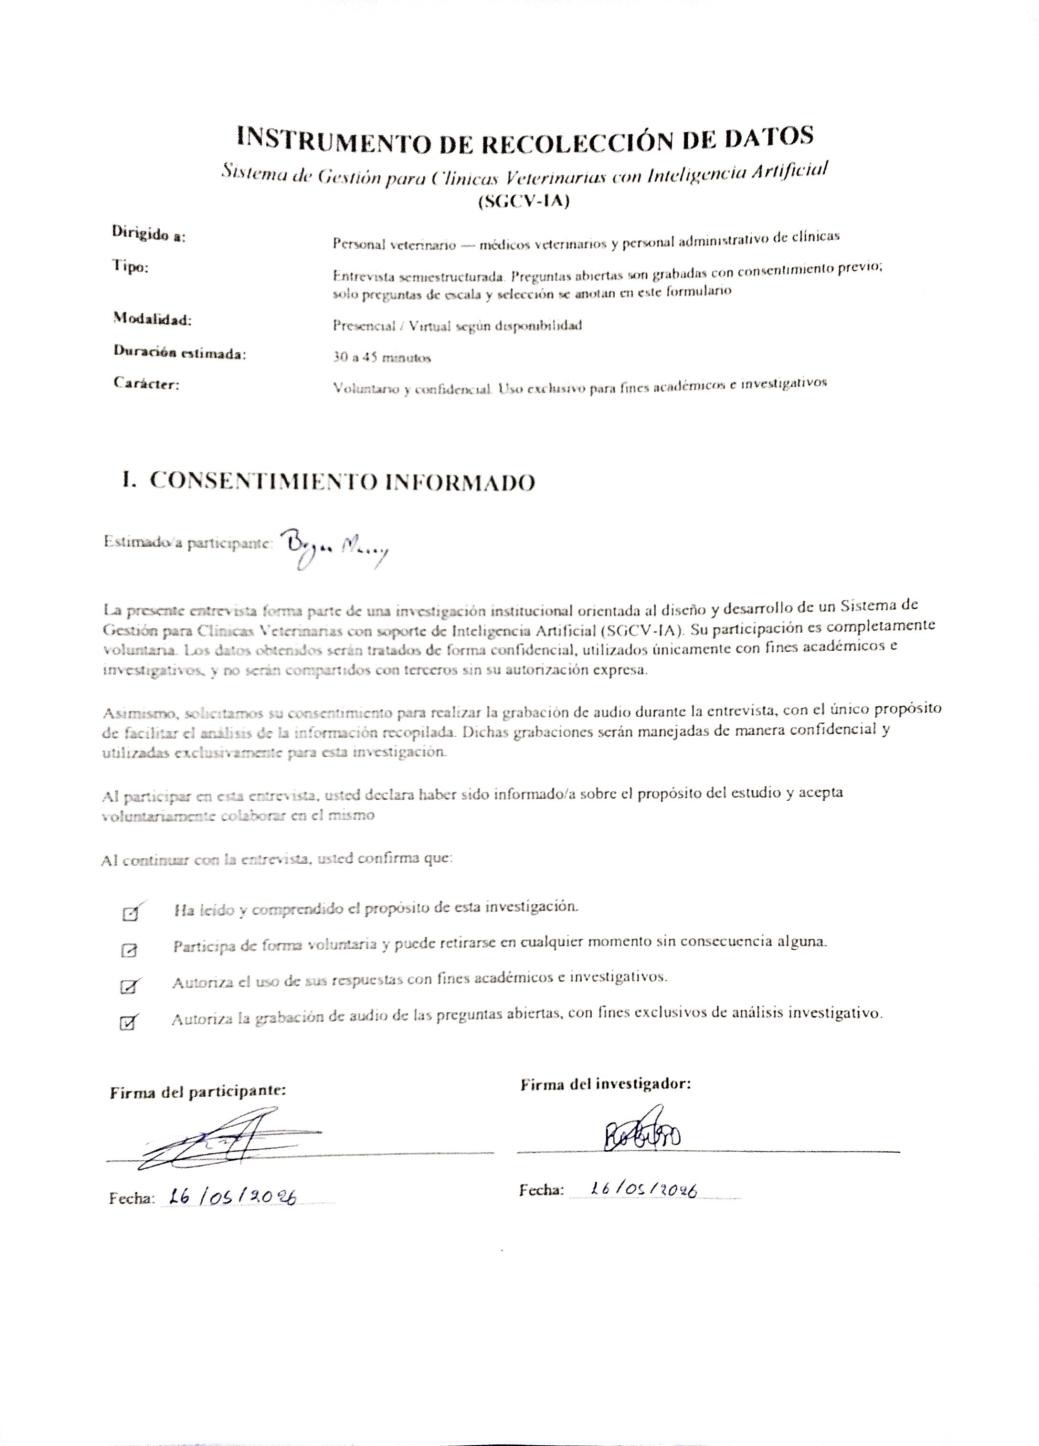
\includegraphics[width=5.19796in,height=7.23in]{./media/image36.jpeg}
\end{quote}

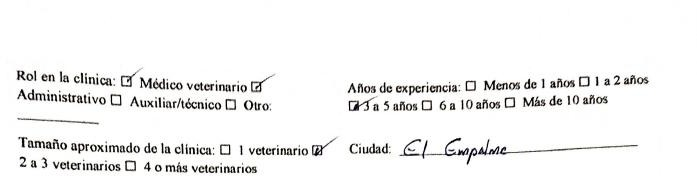
\includegraphics[width=5.44295in,height=1.38281in]{./media/image37.jpeg}

\begin{quote}
\protect\phantomsection\label{_bookmark88}{}Ilustración
25.Consentimiento informado firmado- Dr Bryan Macay
\end{quote}


\includegraphics[width=6.79514in,height=9.61528in]{./media/image38.png}

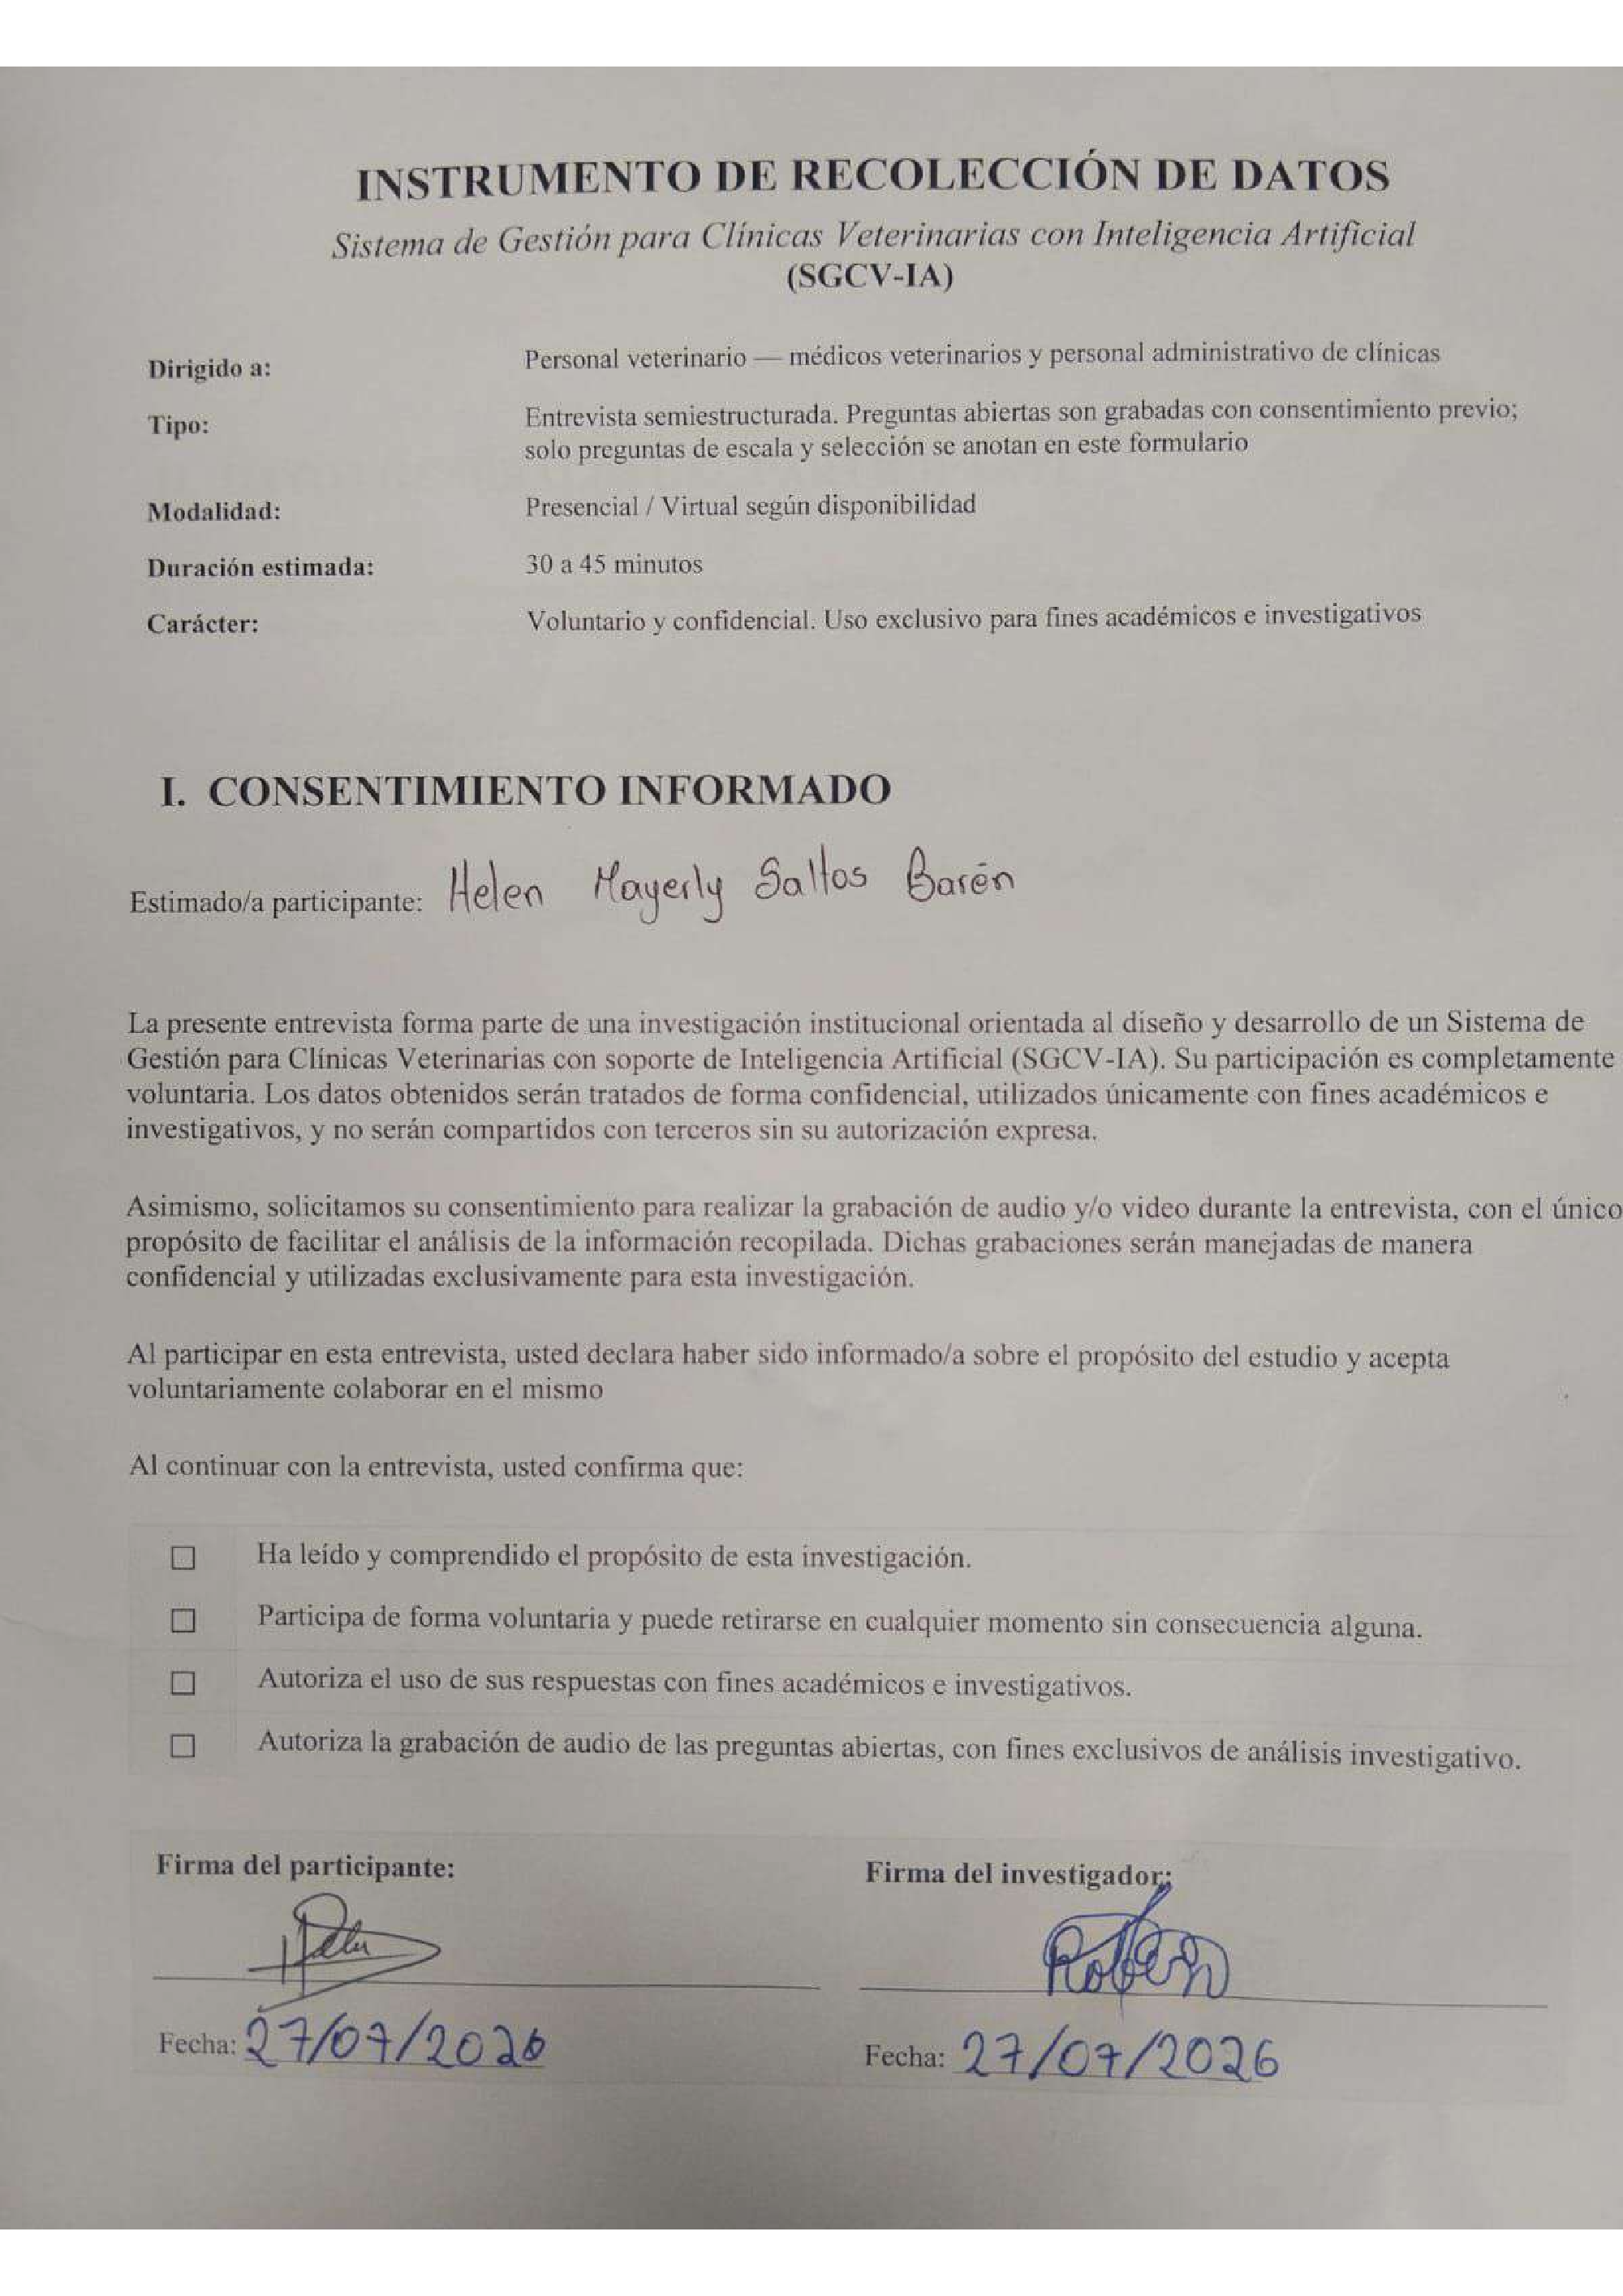
\includegraphics[width=6.79514in,height=9.61528in]{./media/image39.png}
\includegraphics[width=6.79514in,height=9.60833in]{./media/image40.png}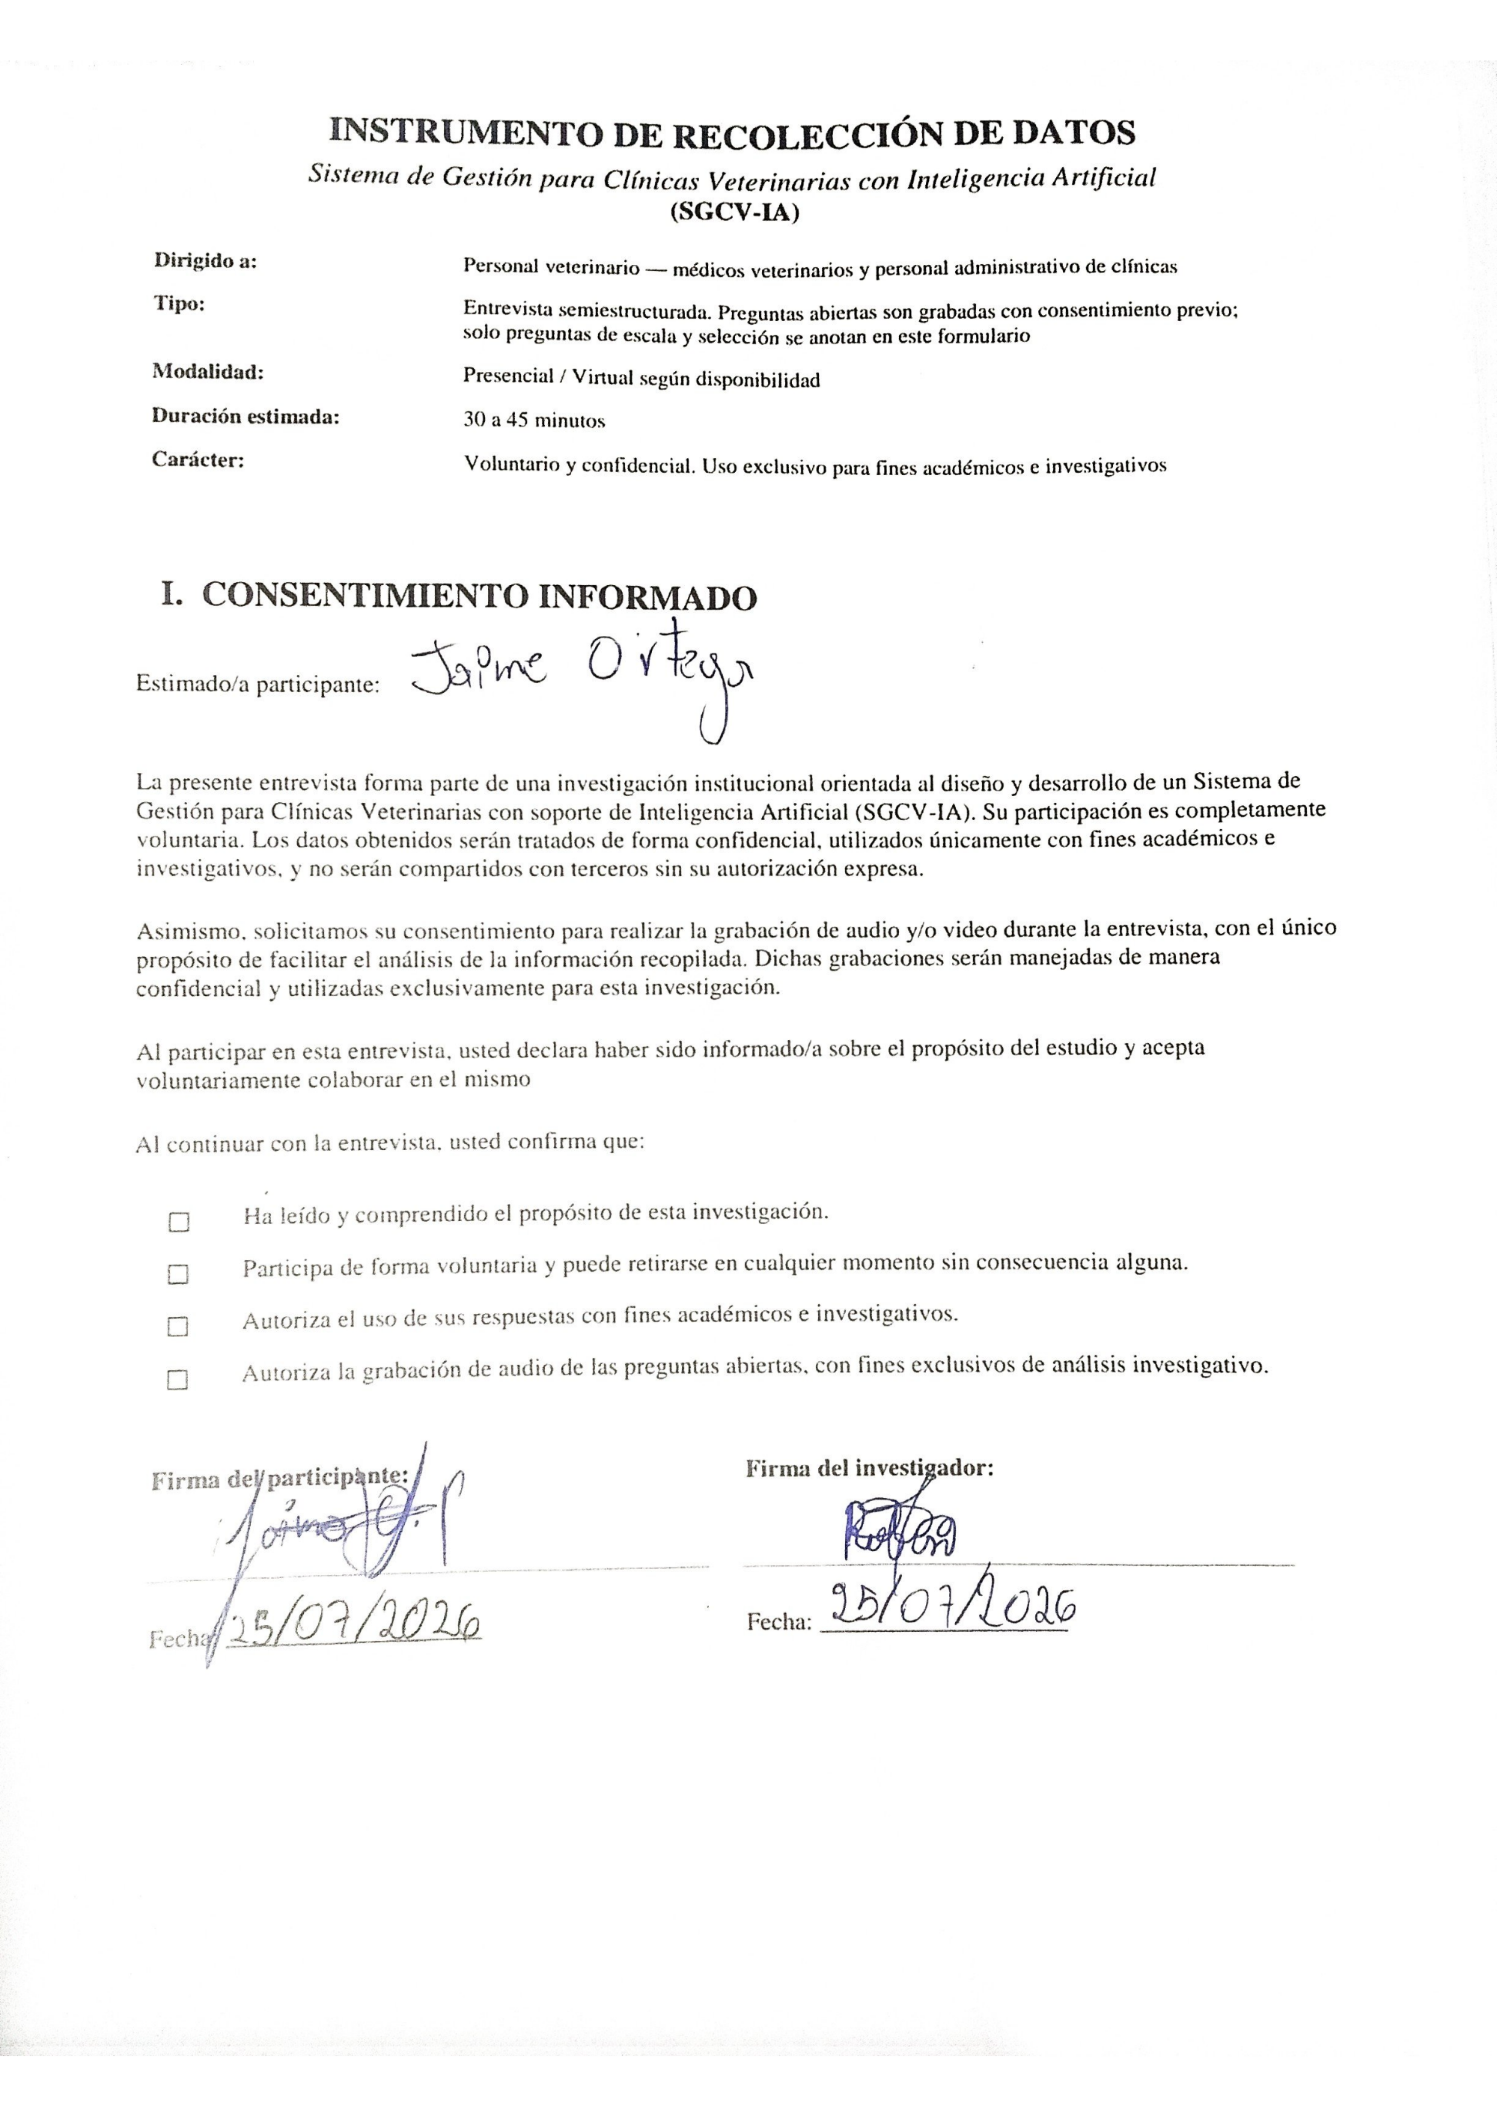
\includegraphics[width=6.79514in,height=9.60833in]{./media/image41.png}
\includegraphics[width=6.79514in,height=9.60833in]{./media/image42.png}
\includegraphics[width=6.79514in,height=9.61528in]{./media/image43.png}
\includegraphics[width=6.79514in,height=9.60833in]{./media/image44.png}

\paragraph{Índice de multimedia con
enlaces}\label{uxedndice-de-multimedia-con-enlaces}

\begin{quote}
Enlace de videos desde el repositorio:

\url{https://github.com/ramaguas-ship-it/SGCV-IA/tree/main/02_Evidencias/Video}

Link directo para los videos de las entrevistas de las clinicas
veterinarias mediante el link directo del repositorio.

\textbf{Eviencias A}
\end{quote}

{\def\LTcaptype{none} % do not increment counter
\begin{longtable}[]{@{}
  >{\raggedright\arraybackslash}p{(\linewidth - 4\tabcolsep) * \real{0.1945}}
  >{\raggedright\arraybackslash}p{(\linewidth - 4\tabcolsep) * \real{0.4379}}
  >{\raggedright\arraybackslash}p{(\linewidth - 4\tabcolsep) * \real{0.3616}}@{}}
\toprule\noalign{}
\begin{minipage}[b]{\linewidth}\centering
\textbf{Evidencia}
\end{minipage} & \begin{minipage}[b]{\linewidth}\centering
\textbf{Descripción}
\end{minipage} & \begin{minipage}[b]{\linewidth}\centering
\textbf{Ubicación en el repositorio}
\end{minipage} \\
\midrule\noalign{}
\endhead
\bottomrule\noalign{}
\endlastfoot
Audios de entrevistas & Grabaciones de las entrevistas realizadas a los
participantes durante la etapa de elicitación de requisitos. &
02\_Evidencias/Audio/ \\
Consentimientos informados & Documentos firmados por los participantes
autorizando el uso de la información recopilada para fines académicos y
de investigación. & 02\_Evidencias/Consentimientos/ \\
Transcripciones & Transcripciones anonimizadas de las entrevistas
utilizadas para el análisis cualitativo. &
02\_Evidencias/Transcripciones/ \\
Fotografías del entorno & Fotografías del entorno de las clínicas
veterinarias y del contexto donde se realizó el levantamiento de
información. & 02\_Evidencias/Fotos\_Entorno/ \\
Documentos de organización & Documentos institucionales proporcionados
por las clínicas veterinarias para comprender sus procesos y
funcionamiento. & 02\_Evidencias/Documentos\_Organizacion/ \\
Cuestionario & Instrumento utilizado para recopilar información
adicional de los participantes y sus respectivas respuestas. &
02\_Evidencias/Cuestionario/ \\
Codificación temática & Archivo con la codificación cualitativa de las
entrevistas, incluyendo fragmentos, códigos, categorías y requisitos
derivados. & 02\_Evidencias/Codificacion\_Tematica/ \\
\end{longtable}
}

\begin{quote}
\textbf{Fotos de evidencia:}

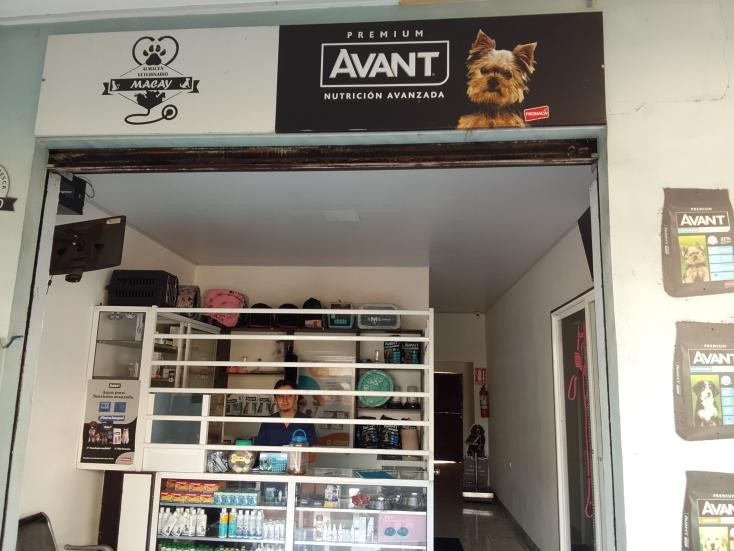
\includegraphics[width=3.67486in,height=2.755in]{./media/image45.jpeg}
\end{quote}

\protect\phantomsection\label{_bookmark90}{}Ilustración 26: Sesión de
entrevista-Veterinaria Macay

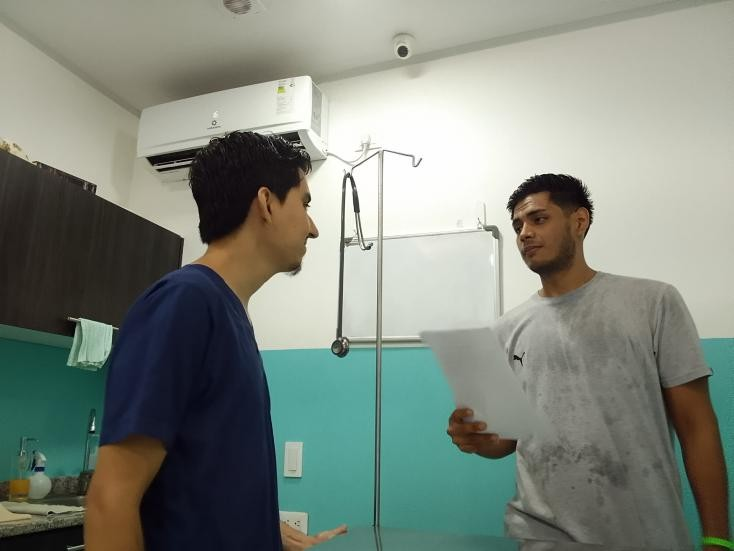
\includegraphics[width=3.67486in,height=2.755in]{./media/image46.jpeg}

\protect\phantomsection\label{_bookmark91}{}Ilustración 27.Sesión de
entrevista-Veterinaria Macay

\begin{quote}
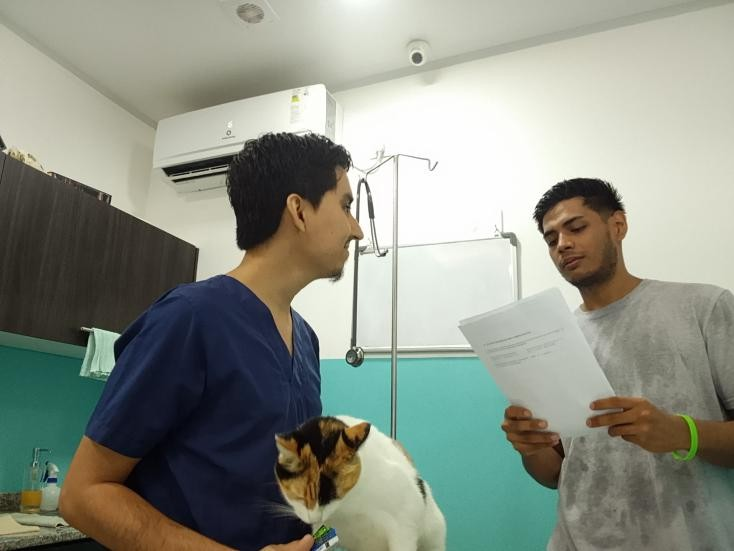
\includegraphics[width=3.67486in,height=2.755in]{./media/image47.jpeg}
\end{quote}

\protect\phantomsection\label{_bookmark92}{}Ilustración 28.Sesión de
entrevista-Veterinaria Macay

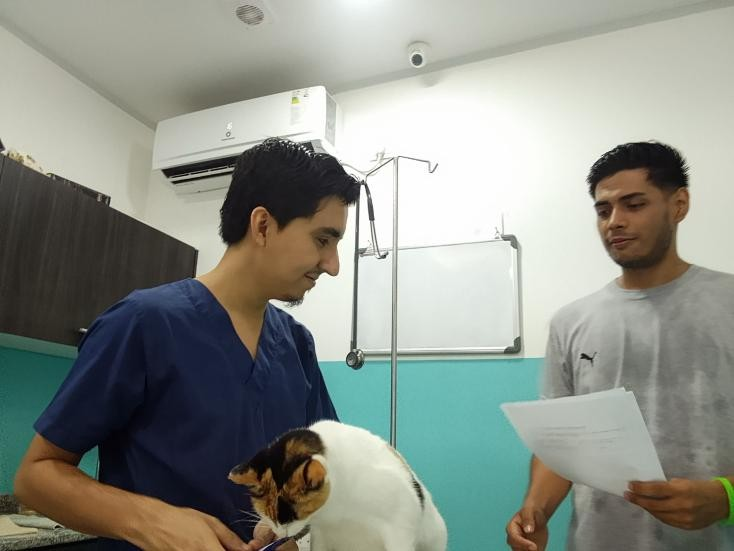
\includegraphics[width=3.67505in,height=2.755in]{./media/image48.jpeg}

\protect\phantomsection\label{_bookmark93}{}Ilustración 29.Sesión de
entrevista-Veterinaria Macay

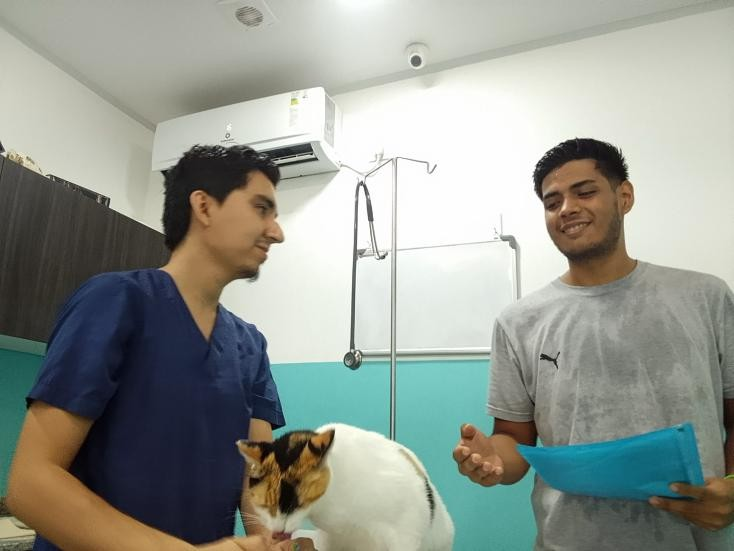
\includegraphics[width=3.67523in,height=2.755in]{./media/image49.jpeg}

\protect\phantomsection\label{_bookmark94}{}Ilustración 30.Sesión de
entrevista-Veterinaria Macay

\begin{quote}
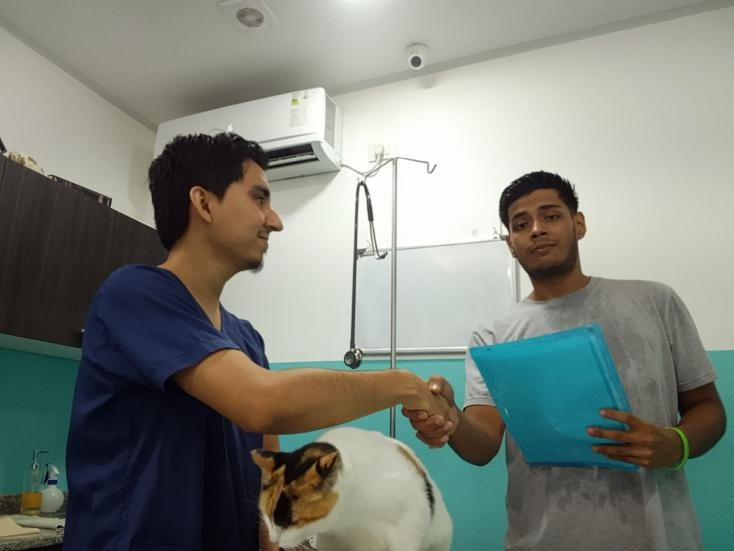
\includegraphics[width=3.67486in,height=2.755in]{./media/image50.jpeg}
\end{quote}

\protect\phantomsection\label{_bookmark95}{}Ilustración 31.Sesión de
entrevista-Veterinaria Macay

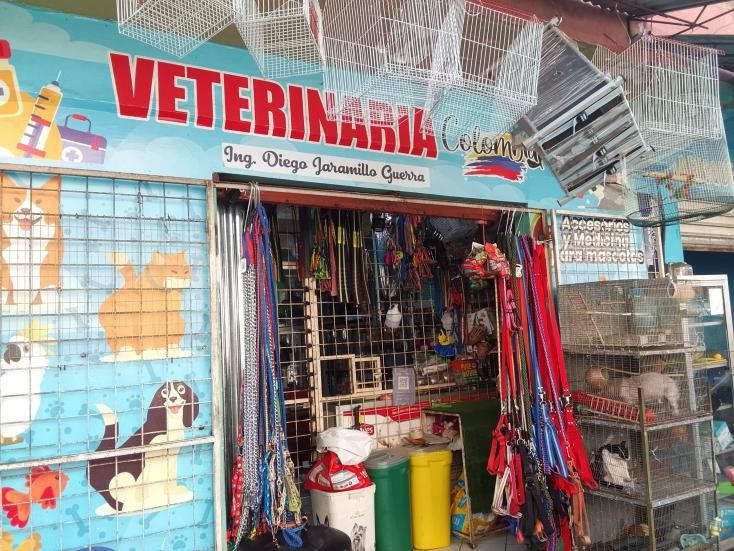
\includegraphics[width=3.67486in,height=2.755in]{./media/image51.jpeg}

\begin{quote}
\protect\phantomsection\label{_bookmark96}{}Ilustración 32.Sesión de
entrevista-Veterinaria Colombia
\end{quote}

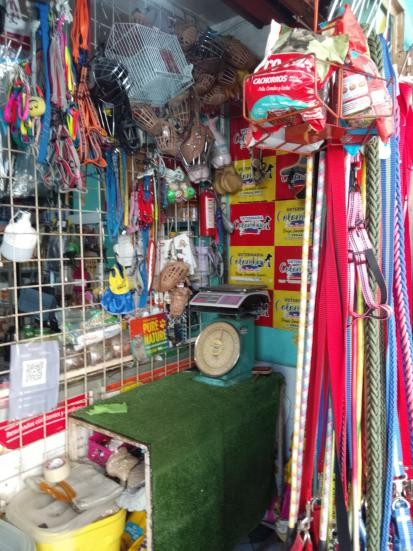
\includegraphics[width=2.06597in,height=2.755in]{./media/image52.jpeg}

\begin{quote}
\protect\phantomsection\label{_bookmark97}{}Ilustración 33.Sesión de
entrevista-Veterinaria Colombia

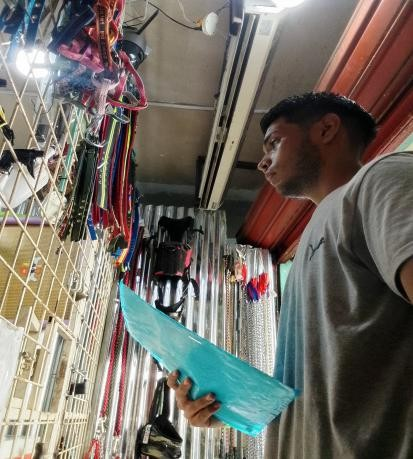
\includegraphics[width=2.06356in,height=2.295in]{./media/image53.jpeg}

\protect\phantomsection\label{_bookmark98}{}Ilustración 34.Sesión de
entrevista-Veterinaria Colombia
\end{quote}

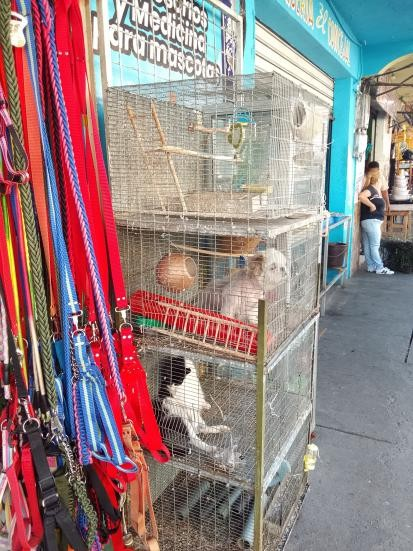
\includegraphics[width=2.06566in,height=2.755in]{./media/image54.jpeg}

\begin{quote}
\protect\phantomsection\label{_bookmark99}{}Ilustración 35.Sesión de
entrevista-Veterinaria Colombia

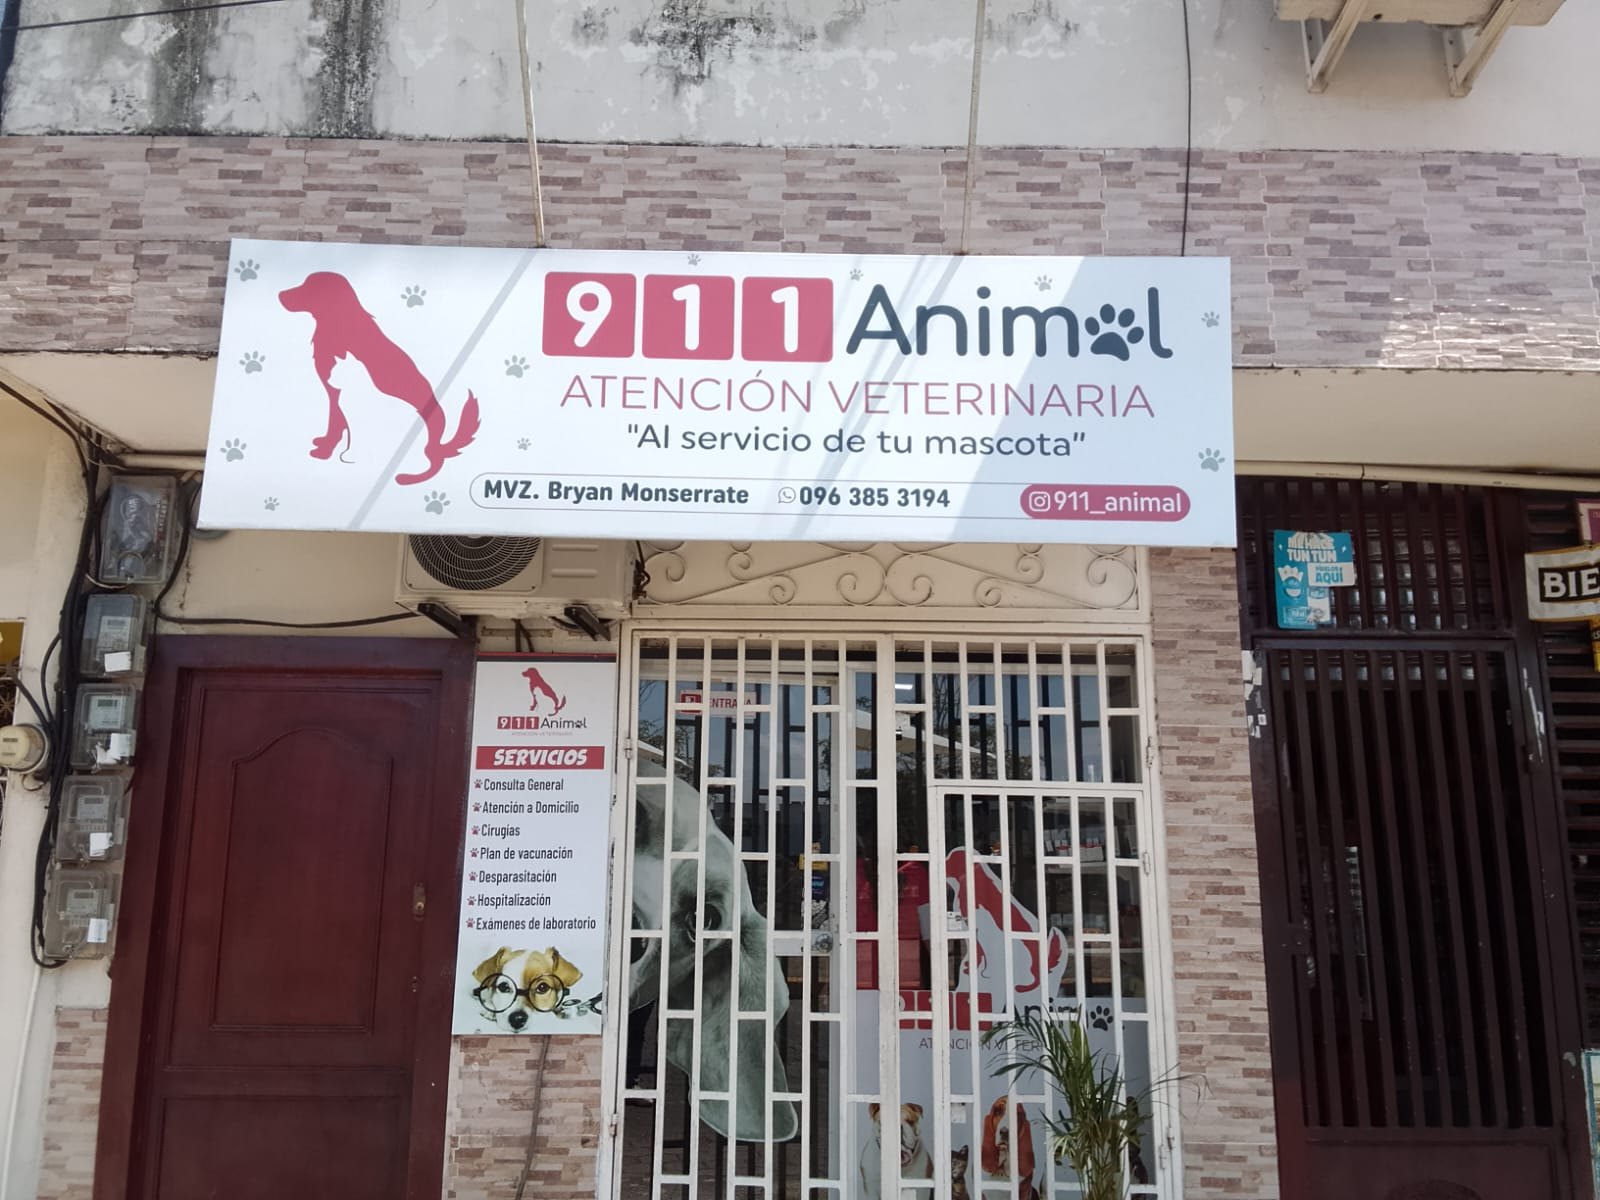
\includegraphics[width=4.58333in,height=3.43762in]{./media/image55.jpeg}
\end{quote}

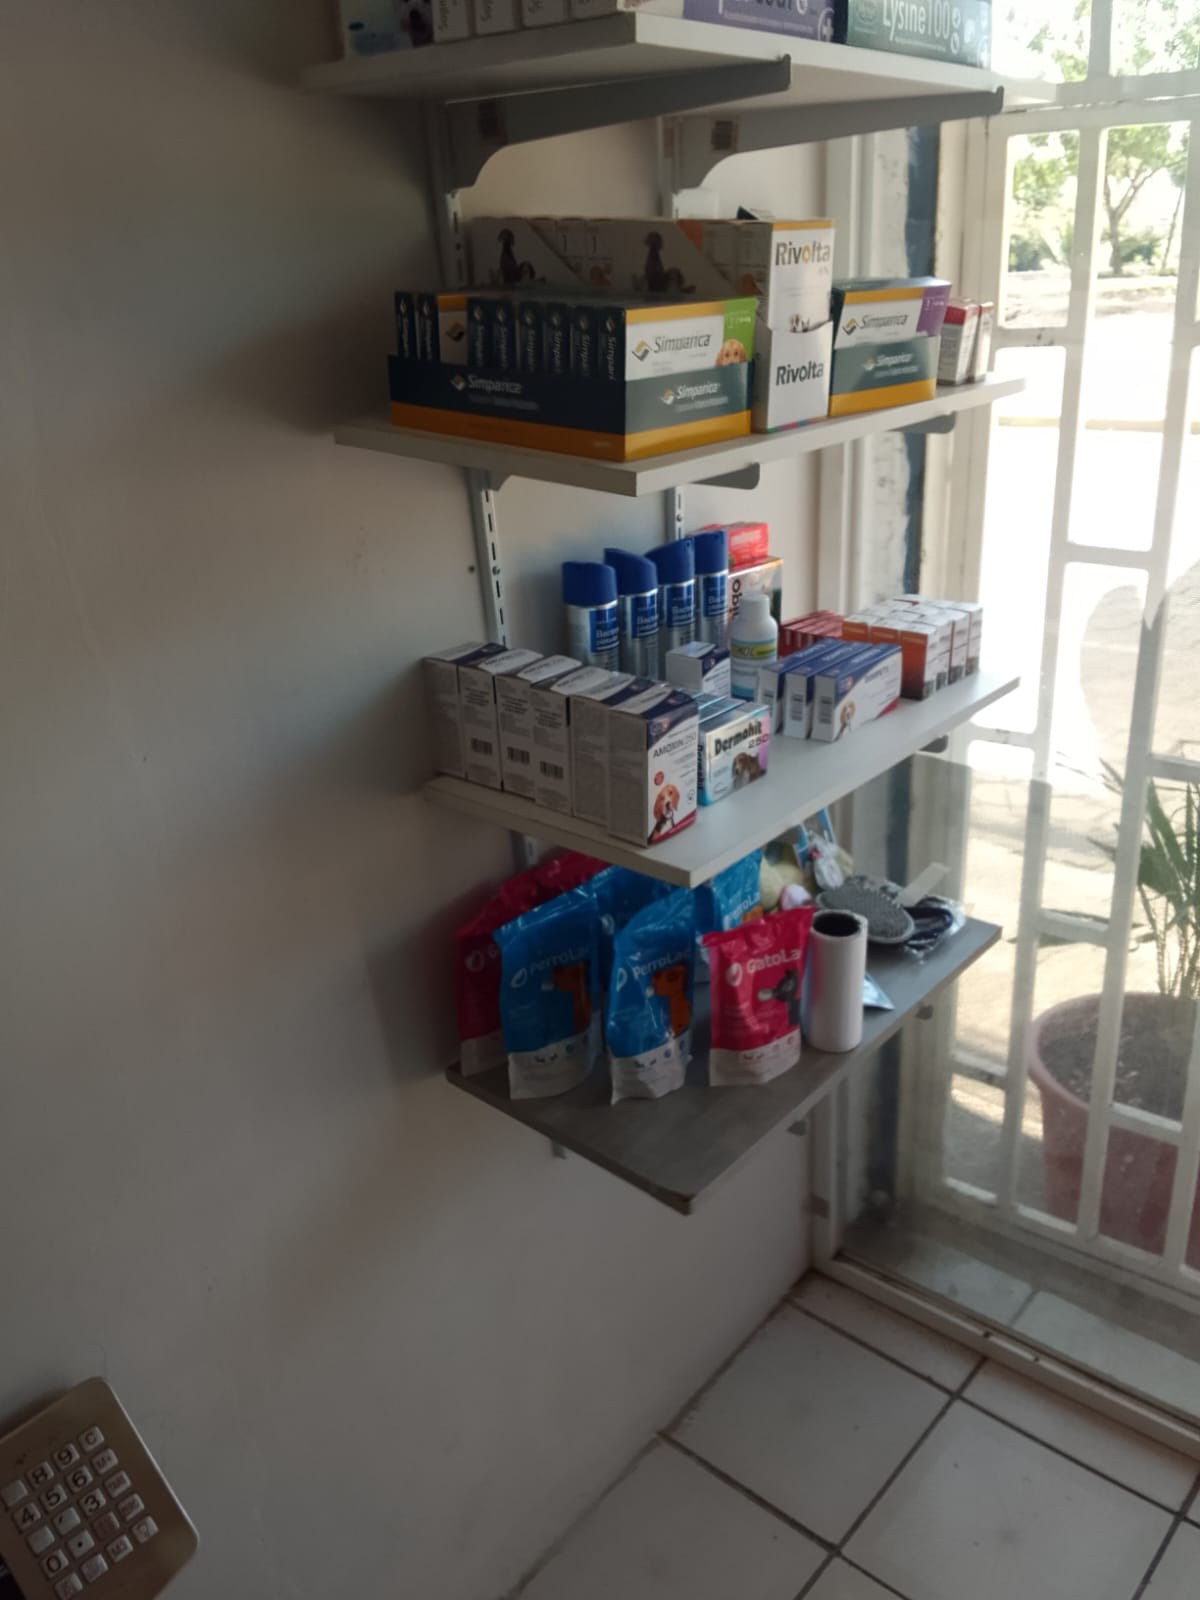
\includegraphics[width=4.15278in,height=5.53718in]{./media/image56.jpeg}

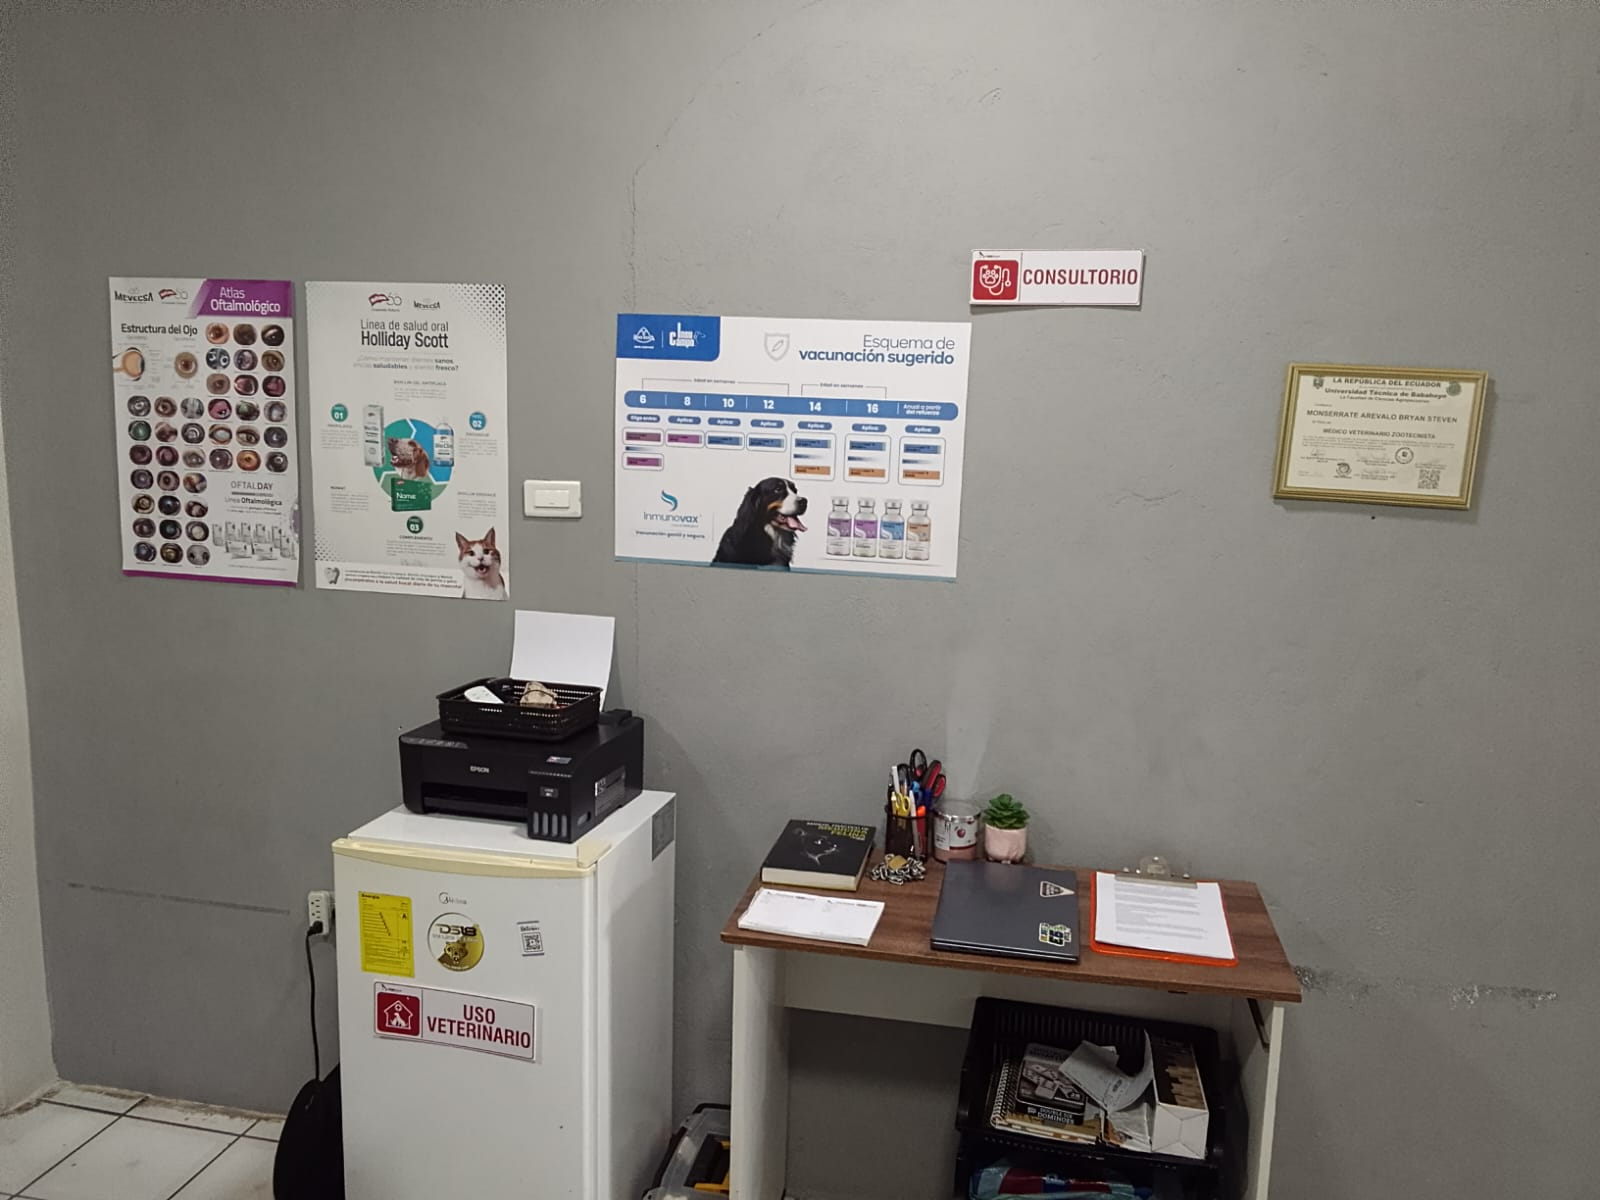
\includegraphics[width=4.05542in,height=3.04167in]{./media/image57.jpeg}

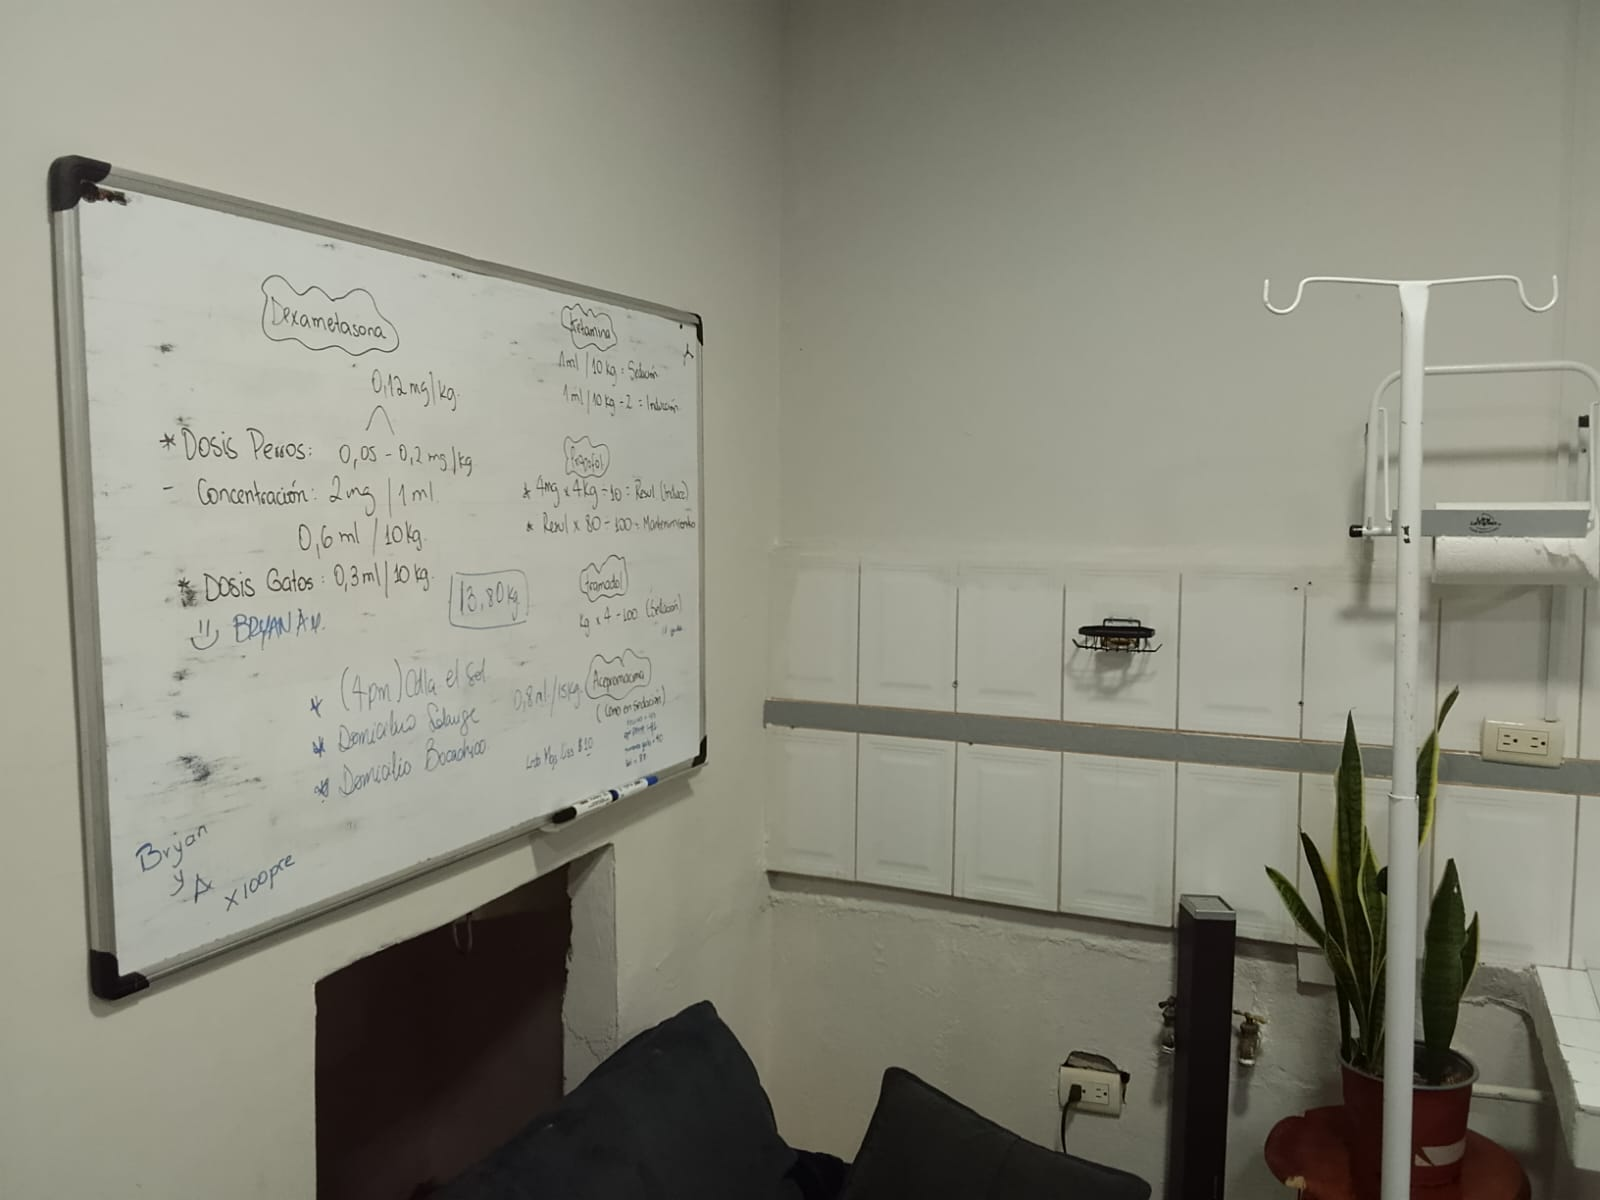
\includegraphics[width=4.61111in,height=3.45845in]{./media/image58.jpeg}


\includegraphics[width=4.73611in,height=3.5522in]{./media/image59.jpeg}

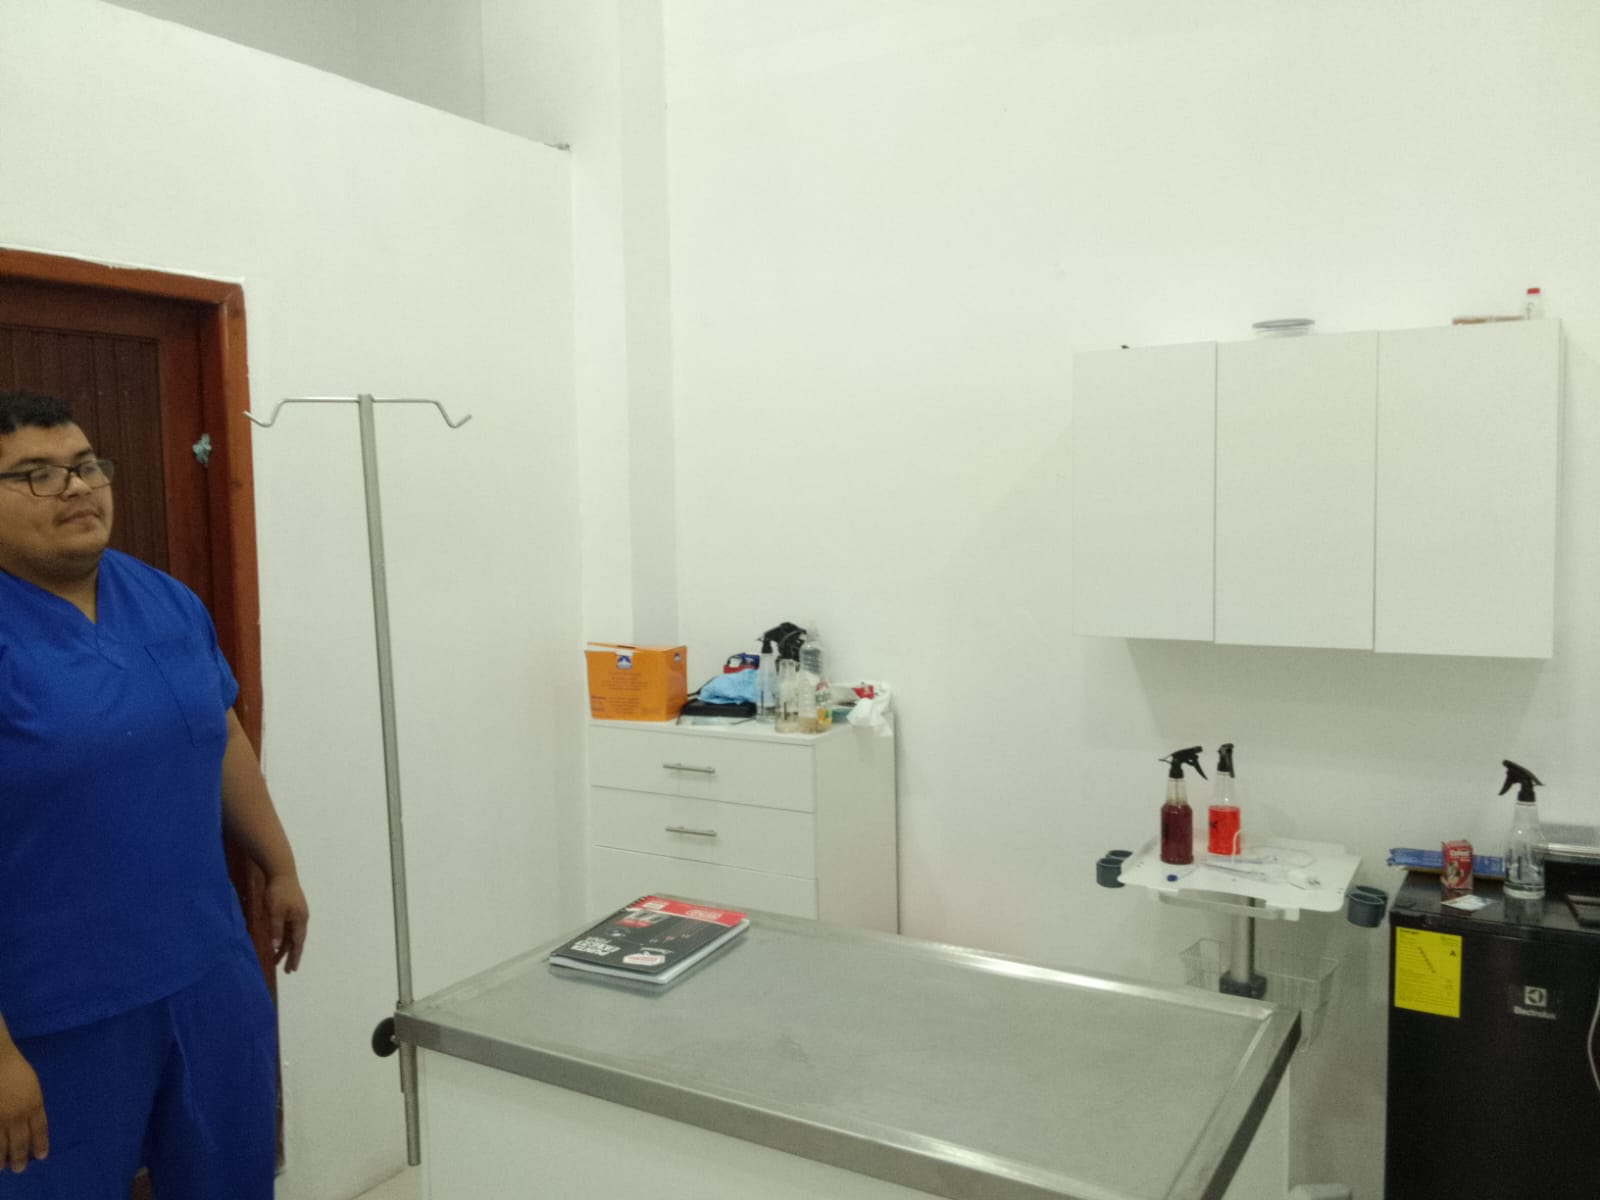
\includegraphics[width=4.98611in,height=3.73971in]{./media/image60.jpeg}

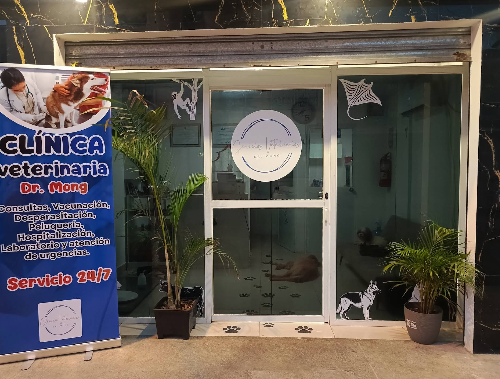
\includegraphics[width=5.20833in,height=3.94444in]{./media/image61.png}

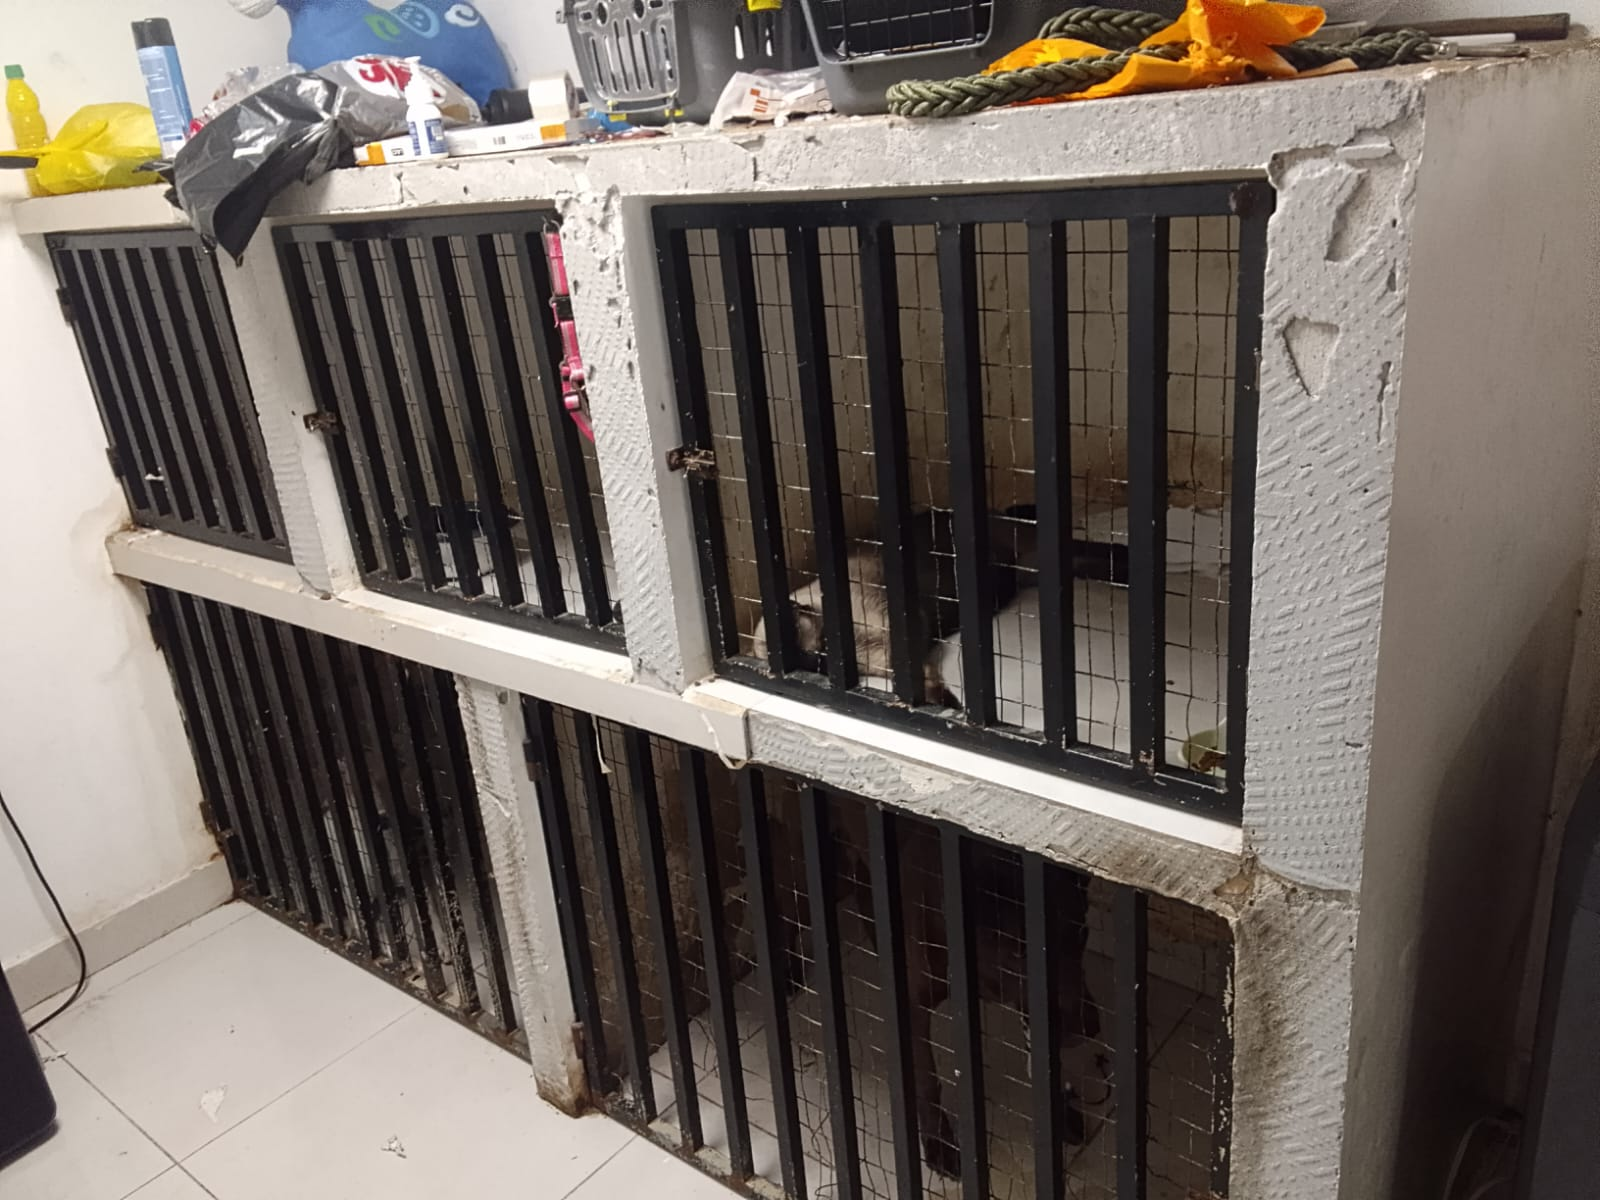
\includegraphics[width=4.68056in,height=3.51054in]{./media/image62.jpeg}

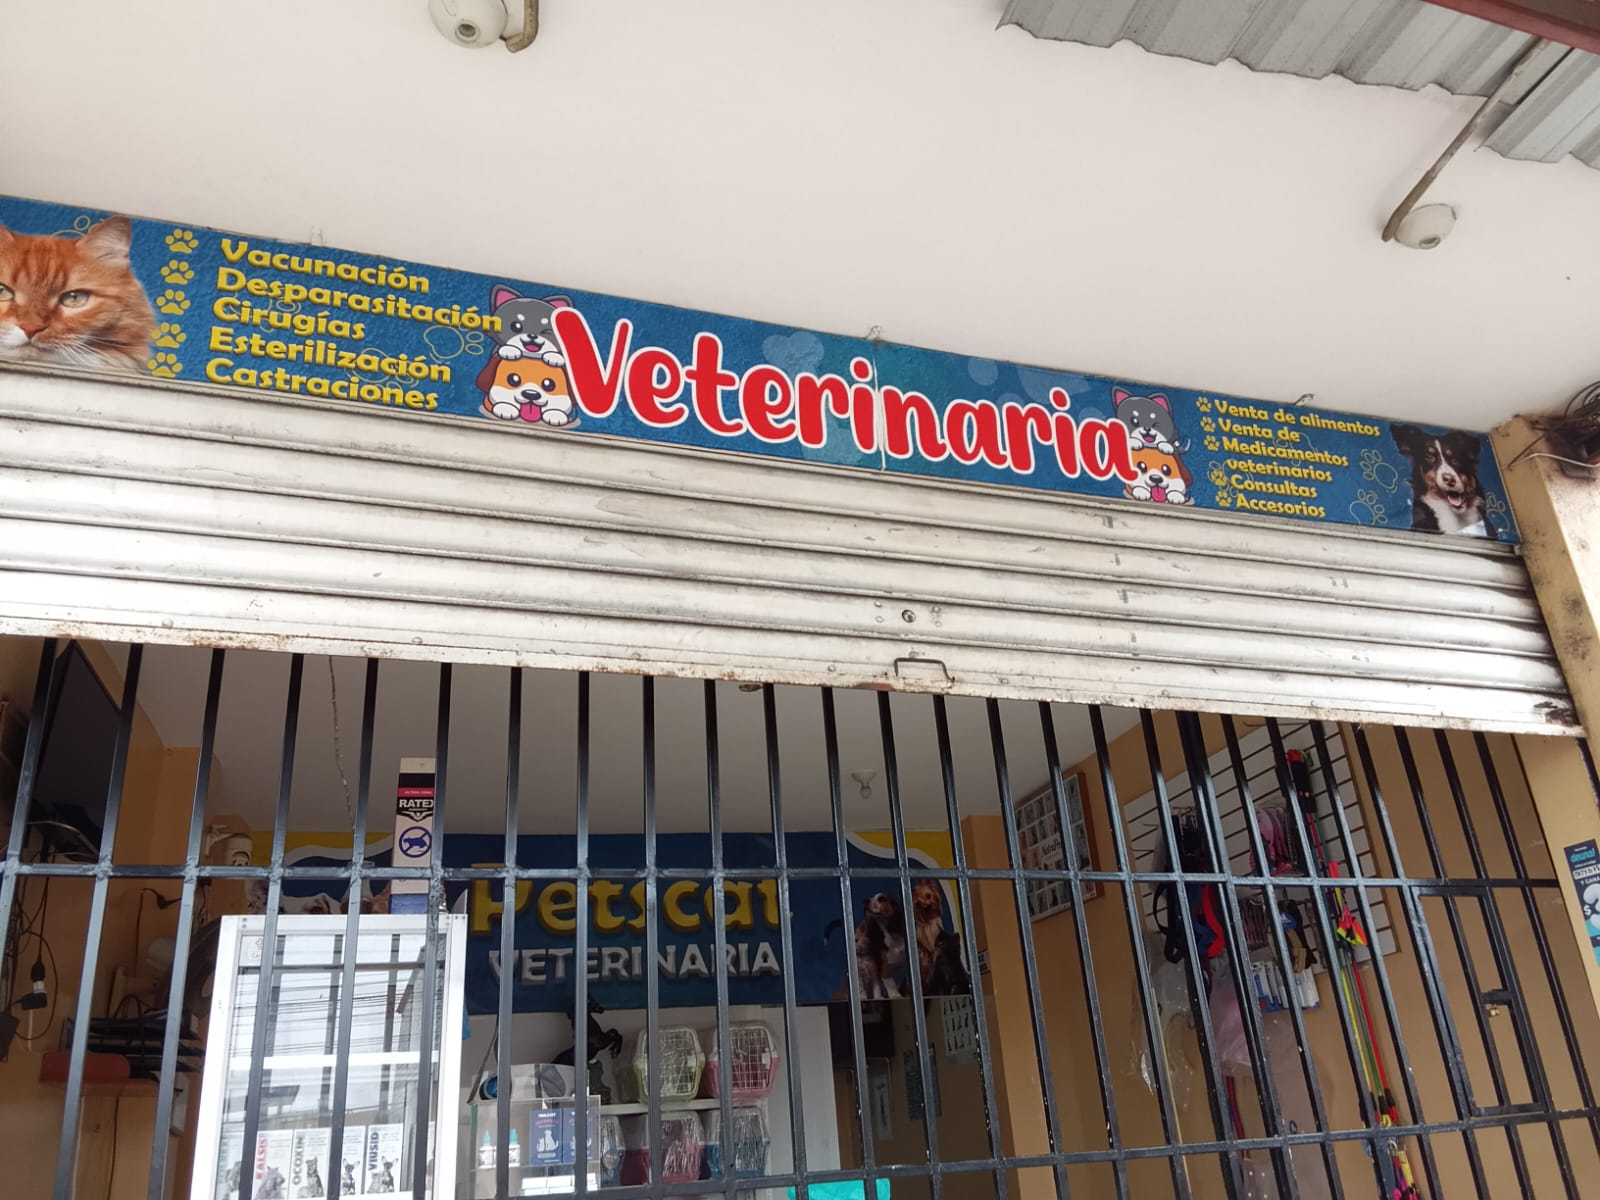
\includegraphics[width=4.99983in,height=3.75in]{./media/image63.jpeg}

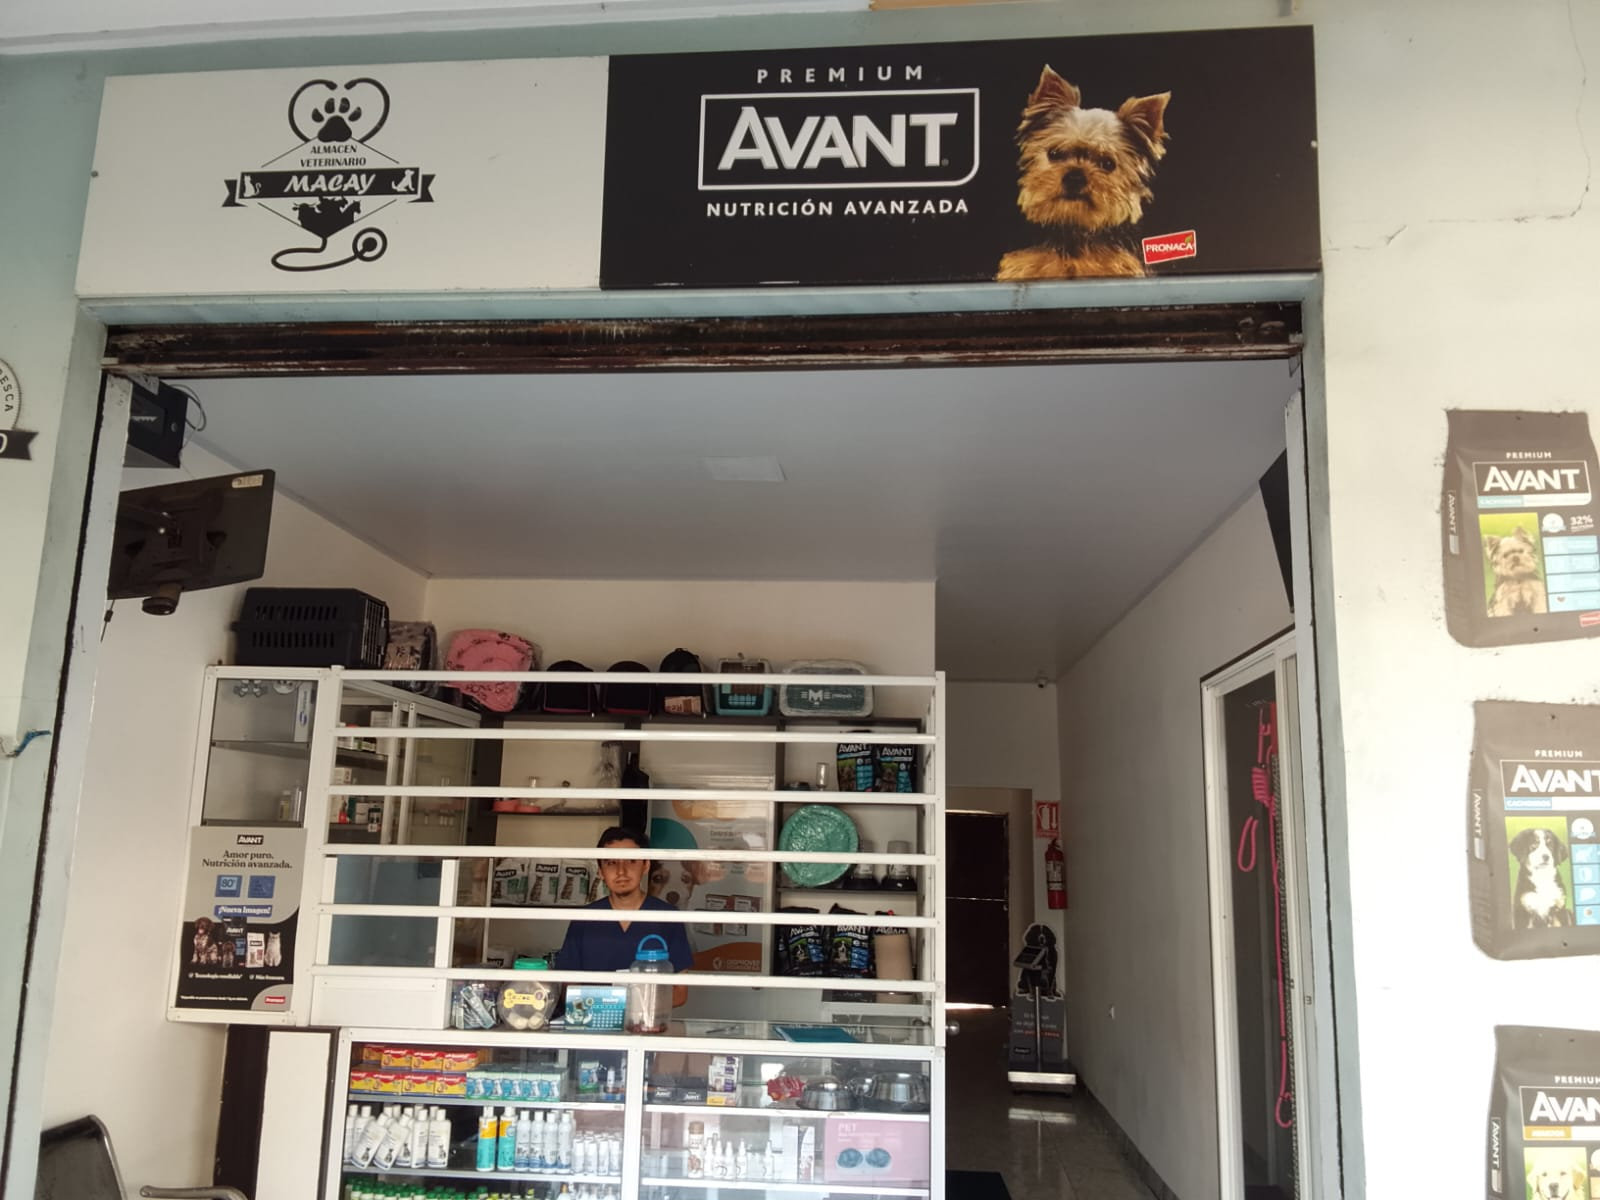
\includegraphics[width=4.56944in,height=3.4272in]{./media/image64.jpeg}

\paragraph{Clasificación y priorización MoSCoW (detalle
completo)}\label{clasificaciuxf3n-y-priorizaciuxf3n-moscow-detalle-completo}

\begin{enumerate}
\def\labelenumi{\arabic{enumi}.}
\item
  \protect\phantomsection\label{_bookmark101}{}\textbf{Clasificación de
  Requisitos}
\end{enumerate}

\begin{quote}
Se clasifican los tres tipos de artefactos identificados en este
documento: Requisitos Funcionales (RF), Requisitos No Funcionales (RNF)
y Restricciones (RST), para un total de 40 elementos.
\end{quote}

{\def\LTcaptype{none} % do not increment counter
\begin{longtable}[]{@{}
  >{\raggedright\arraybackslash}p{(\linewidth - 6\tabcolsep) * \real{0.2394}}
  >{\centering\arraybackslash}p{(\linewidth - 6\tabcolsep) * \real{0.1940}}
  >{\centering\arraybackslash}p{(\linewidth - 6\tabcolsep) * \real{0.2845}}
  >{\centering\arraybackslash}p{(\linewidth - 6\tabcolsep) * \real{0.2395}}@{}}
\toprule\noalign{}
\begin{minipage}[b]{\linewidth}\centering
\textbf{Tipo}
\end{minipage} & \begin{minipage}[b]{\linewidth}\centering
\textbf{Cantidad}
\end{minipage} & \begin{minipage}[b]{\linewidth}\centering
\textbf{Rango de IDs}
\end{minipage} & \begin{minipage}[b]{\linewidth}\centering
\textbf{Sección de origen}
\end{minipage} \\
\midrule\noalign{}
\endhead
\bottomrule\noalign{}
\endlastfoot
\begin{minipage}[t]{\linewidth}\raggedright
\begin{quote}
Requisito Funcional (RF)
\end{quote}
\end{minipage} & 24 & RF-01 a RF-24 & Sección 3.2 \\
\begin{minipage}[t]{\linewidth}\raggedright
\begin{quote}
Requisito No Funcional (RNF)
\end{quote}
\end{minipage} & 10 & RNF-01 a RNF-10 & Sección 3.3 \\
Restricción (RST) & 6 & RST-01 a RST-06 & Secciones 2.6 / 3.4 \\
\end{longtable}
}

\protect\phantomsection\label{_bookmark102}{}\emph{\textbf{Tabla 25.
Clasificación de Requisitos}}

\paragraph{Detalle de Restricciones
clasificadas}\label{detalle-de-restricciones-clasificadas}

\paragraph{}\label{section-11}

{\def\LTcaptype{none} % do not increment counter
\begin{longtable}[]{@{}
  >{\raggedright\arraybackslash}p{(\linewidth - 4\tabcolsep) * \real{0.1155}}
  >{\raggedright\arraybackslash}p{(\linewidth - 4\tabcolsep) * \real{0.5219}}
  >{\raggedright\arraybackslash}p{(\linewidth - 4\tabcolsep) * \real{0.3188}}@{}}
\toprule\noalign{}
\begin{minipage}[b]{\linewidth}\centering
\textbf{ID}
\end{minipage} & \begin{minipage}[b]{\linewidth}\centering
\textbf{Restricción}
\end{minipage} & \begin{minipage}[b]{\linewidth}\centering
\textbf{Tipo}
\end{minipage} \\
\midrule\noalign{}
\endhead
\bottomrule\noalign{}
\endlastfoot
RST-01 & Base de datos relacional (PostgreSQL/MySQL); sin NoSQL como
almacenamiento principal. & \begin{minipage}[t]{\linewidth}\raggedright
\begin{quote}
Tecnológica
\end{quote}
\end{minipage} \\
RST-02 & Cumplimiento de la normativa ecuatoriana de protección de datos
personales (LOPDP). & \begin{minipage}[t]{\linewidth}\raggedright
\begin{quote}
Regulatoria
\end{quote}
\end{minipage} \\
RST-03 & Autenticación y control de acceso basado en roles (RBAC)
obligatorios. & \begin{minipage}[t]{\linewidth}\raggedright
\begin{quote}
Seguridad
\end{quote}
\end{minipage} \\
RST-04 & Priorización de frameworks y bibliotecas de código abierto. &
\begin{minipage}[t]{\linewidth}\raggedright
\begin{quote}
Presupuestaria
\end{quote}
\end{minipage} \\
RST-05 & Arquitectura cliente-servidor con API REST; módulo de IA
desacoplado del backend. & \begin{minipage}[t]{\linewidth}\raggedright
\begin{quote}
Arquitectónica
\end{quote}
\end{minipage} \\
RST-06 & Sincronización offline mediante cola local de operaciones, no
réplica completa de BD en

cliente. & \begin{minipage}[t]{\linewidth}\raggedright
\begin{quote}
Técnica / Hardware
\end{quote}
\end{minipage} \\
\end{longtable}
}

\protect\phantomsection\label{_bookmark103}{}\emph{\textbf{Tabla 26.
Detalle de Restricciones clasificadas}}

\paragraph{Priorización MoSCoW por Requisito
Funcional}\label{priorizaciuxf3n-moscow-por-requisito-funcional}

\paragraph{}\label{section-12}

{\def\LTcaptype{none} % do not increment counter
\begin{longtable}[]{@{}
  >{\raggedleft\arraybackslash}p{(\linewidth - 4\tabcolsep) * \real{0.1155}}
  >{\raggedright\arraybackslash}p{(\linewidth - 4\tabcolsep) * \real{0.5219}}
  >{\raggedright\arraybackslash}p{(\linewidth - 4\tabcolsep) * \real{0.3188}}@{}}
\toprule\noalign{}
\begin{minipage}[b]{\linewidth}\raggedleft
\textbf{ID}
\end{minipage} & \begin{minipage}[b]{\linewidth}\centering
\textbf{Nombre del RF}
\end{minipage} & \begin{minipage}[b]{\linewidth}\centering
\textbf{Prioridad}
\end{minipage} \\
\midrule\noalign{}
\endhead
\bottomrule\noalign{}
\endlastfoot
RF-01 & Registro de paciente &
\begin{minipage}[t]{\linewidth}\raggedright
\begin{quote}
Must have
\end{quote}
\end{minipage} \\
RF-02 & Búsqueda rápida por nombre del paciente y dueño &
\begin{minipage}[t]{\linewidth}\raggedright
\begin{quote}
Must have
\end{quote}
\end{minipage} \\
RF-03 & Registro detallado de historial clínico &
\begin{minipage}[t]{\linewidth}\raggedright
\begin{quote}
Must have
\end{quote}
\end{minipage} \\
RF-04 & Actualización de historial clínico &
\begin{minipage}[t]{\linewidth}\raggedright
\begin{quote}
Must have
\end{quote}
\end{minipage} \\
RF-05 & Control de inventario con alertas de vencimiento &
\begin{minipage}[t]{\linewidth}\raggedright
\begin{quote}
Must have
\end{quote}
\end{minipage} \\
RF-06 & Gestión de stock con alertas de faltantes &
\begin{minipage}[t]{\linewidth}\raggedright
\begin{quote}
Must have
\end{quote}
\end{minipage} \\
RF-07 & Registro del proceso de cobro &
\begin{minipage}[t]{\linewidth}\raggedright
\begin{quote}
Must have
\end{quote}
\end{minipage} \\
RF-08 & Módulo de facturación ágil &
\begin{minipage}[t]{\linewidth}\raggedright
\begin{quote}
Must have
\end{quote}
\end{minipage} \\
RF-09 & Registro de comunicaciones post-consulta &
\begin{minipage}[t]{\linewidth}\raggedright
\begin{quote}
Must have
\end{quote}
\end{minipage} \\
RF-10 & Envío de resultados por WhatsApp &
\begin{minipage}[t]{\linewidth}\raggedright
\begin{quote}
Must have
\end{quote}
\end{minipage} \\
RF-11 & Registro de citas e inasistencias &
\begin{minipage}[t]{\linewidth}\raggedright
\begin{quote}
Must have
\end{quote}
\end{minipage} \\
RF-12 & Recordatorios automáticos de citas &
\begin{minipage}[t]{\linewidth}\raggedright
\begin{quote}
Must have
\end{quote}
\end{minipage} \\
RF-13 & Registro de parámetros de crecimiento y peso &
\begin{minipage}[t]{\linewidth}\raggedright
\begin{quote}
Must have
\end{quote}
\end{minipage} \\
RF-14 & Generación de recomendaciones nutricionales personalizadas &
\begin{minipage}[t]{\linewidth}\raggedright
\begin{quote}
Must have
\end{quote}
\end{minipage} \\
RF-15 & Programación de recordatorios de seguimiento médico &
\begin{minipage}[t]{\linewidth}\raggedright
\begin{quote}
Must have
\end{quote}
\end{minipage} \\
RF-16 & Exportación de reportes de salud del paciente &
\begin{minipage}[t]{\linewidth}\raggedright
\begin{quote}
Must have
\end{quote}
\end{minipage} \\
RF-17 & Sugerencias diagnósticas basadas en datos clínicos (con
validación obligatoria) & \begin{minipage}[t]{\linewidth}\raggedright
\begin{quote}
Must have
\end{quote}
\end{minipage} \\
RF-18 & Respaldo de recomendaciones en literatura científica veterinaria
validada & \begin{minipage}[t]{\linewidth}\raggedright
\begin{quote}
Should have
\end{quote}
\end{minipage} \\
RF-19 & Capacidad de revisión y corrección de sugerencias de IA por
parte del veterinario & \begin{minipage}[t]{\linewidth}\raggedright
\begin{quote}
Should have
\end{quote}
\end{minipage} \\
RF-20 & Interfaz sencilla sin capacitación prolongada &
\begin{minipage}[t]{\linewidth}\raggedright
\begin{quote}
Should have
\end{quote}
\end{minipage} \\
RF-21 & Operación con baja dependencia de conectividad permanente &
\begin{minipage}[t]{\linewidth}\raggedright
\begin{quote}
Should have
\end{quote}
\end{minipage} \\
RF-22 & Bajo costo de implementación y operación &
\begin{minipage}[t]{\linewidth}\raggedright
\begin{quote}
Should have
\end{quote}
\end{minipage} \\
RF-23 & Perfiles de usuario diferenciados con control de acceso &
\begin{minipage}[t]{\linewidth}\raggedright
\begin{quote}
Should have
\end{quote}
\end{minipage} \\
RF-24 & Trazabilidad de cambios en historiales clínicos &
\begin{minipage}[t]{\linewidth}\raggedright
\begin{quote}
Could have
\end{quote}
\end{minipage} \\
\end{longtable}
}

\begin{quote}
\protect\phantomsection\label{_bookmark104}{}\emph{\textbf{Tabla 27.
MoSCoW por Requisito Funcional}}
\end{quote}

\paragraph{Priorización MoSCoW por Requisito No
Funcional}\label{priorizaciuxf3n-moscow-por-requisito-no-funcional}

{\def\LTcaptype{none} % do not increment counter
\begin{longtable}[]{@{}
  >{\raggedright\arraybackslash}p{(\linewidth - 4\tabcolsep) * \real{0.1157}}
  >{\raggedright\arraybackslash}p{(\linewidth - 4\tabcolsep) * \real{0.5219}}
  >{\raggedright\arraybackslash}p{(\linewidth - 4\tabcolsep) * \real{0.3186}}@{}}
\toprule\noalign{}
\begin{minipage}[b]{\linewidth}\centering
\textbf{ID}
\end{minipage} & \begin{minipage}[b]{\linewidth}\raggedright
\begin{quote}
\textbf{Nombre del NFR}
\end{quote}
\end{minipage} & \begin{minipage}[b]{\linewidth}\centering
\textbf{Prioridad}
\end{minipage} \\
\midrule\noalign{}
\endhead
\bottomrule\noalign{}
\endlastfoot
RNF-01 & \begin{minipage}[t]{\linewidth}\raggedright
\begin{quote}
Eficiencia de desempeño (Tiempo de respuesta)
\end{quote}
\end{minipage} & \begin{minipage}[t]{\linewidth}\raggedright
\begin{quote}
Must have
\end{quote}
\end{minipage} \\
RNF-02 & \begin{minipage}[t]{\linewidth}\raggedright
\begin{quote}
Eficiencia de desempeño (Comportamiento temporal - facturación)
\end{quote}
\end{minipage} & \begin{minipage}[t]{\linewidth}\raggedright
\begin{quote}
Must have
\end{quote}
\end{minipage} \\
RNF-03 & \begin{minipage}[t]{\linewidth}\raggedright
\begin{quote}
Fiabilidad (Madurez - alertas de vencimiento)
\end{quote}
\end{minipage} & \begin{minipage}[t]{\linewidth}\raggedright
\begin{quote}
Should have
\end{quote}
\end{minipage} \\
RNF-04 & \begin{minipage}[t]{\linewidth}\raggedright
\begin{quote}
Fiabilidad (Disponibilidad - operación offline)
\end{quote}
\end{minipage} & \begin{minipage}[t]{\linewidth}\raggedright
\begin{quote}
Must have
\end{quote}
\end{minipage} \\
RNF-05 & \begin{minipage}[t]{\linewidth}\raggedright
\begin{quote}
Seguridad (Control de acceso / Confidencialidad)
\end{quote}
\end{minipage} & \begin{minipage}[t]{\linewidth}\raggedright
\begin{quote}
Must have
\end{quote}
\end{minipage} \\
RNF-06 & \begin{minipage}[t]{\linewidth}\raggedright
\begin{quote}
Seguridad (Trazabilidad / No repudio)
\end{quote}
\end{minipage} & \begin{minipage}[t]{\linewidth}\raggedright
\begin{quote}
Should have
\end{quote}
\end{minipage} \\
RNF-07 & \begin{minipage}[t]{\linewidth}\raggedright
\begin{quote}
Usabilidad (Capacidad de aprendizaje)
\end{quote}
\end{minipage} & \begin{minipage}[t]{\linewidth}\raggedright
\begin{quote}
Should have
\end{quote}
\end{minipage} \\
RNF-08 & \begin{minipage}[t]{\linewidth}\raggedright
\begin{quote}
Compatibilidad (Coexistencia operativa / Portabilidad)
\end{quote}
\end{minipage} & \begin{minipage}[t]{\linewidth}\raggedright
\begin{quote}
Could have
\end{quote}
\end{minipage} \\
\end{longtable}
}

{\def\LTcaptype{none} % do not increment counter
\begin{longtable}[]{@{}
  >{\raggedright\arraybackslash}p{(\linewidth - 4\tabcolsep) * \real{0.1157}}
  >{\raggedright\arraybackslash}p{(\linewidth - 4\tabcolsep) * \real{0.5219}}
  >{\raggedright\arraybackslash}p{(\linewidth - 4\tabcolsep) * \real{0.3186}}@{}}
\toprule\noalign{}
\begin{minipage}[b]{\linewidth}\raggedright
RNF-09
\end{minipage} & \begin{minipage}[b]{\linewidth}\raggedright
\begin{quote}
Fiabilidad / Adecuación funcional (Exactitud de la IA)
\end{quote}
\end{minipage} & \begin{minipage}[b]{\linewidth}\raggedright
\begin{quote}
Must have
\end{quote}
\end{minipage} \\
\midrule\noalign{}
\endhead
\bottomrule\noalign{}
\endlastfoot
RNF-10 & \begin{minipage}[t]{\linewidth}\raggedright
\begin{quote}
Mantenibilidad (Modularidad - desacoplamiento de IA)
\end{quote}
\end{minipage} & \begin{minipage}[t]{\linewidth}\raggedright
\begin{quote}
Could have
\end{quote}
\end{minipage} \\
\end{longtable}
}

\begin{quote}
\protect\phantomsection\label{_bookmark106}{}\emph{\textbf{Tabla 28.
MoSCoW por Requisito No Funcional}}
\end{quote}

\begin{enumerate}
\def\labelenumi{\arabic{enumi}.}
\setcounter{enumi}{4}
\item
  \protect\phantomsection\label{_bookmark107}{}\textbf{Justificación de
  los Extremos (Must y Won\textquotesingle t)}
  \protect\phantomsection\label{_bookmark108}{}\textbf{Justificación de
  Must have (17 RF + 5 NFR)}
\end{enumerate}

\begin{quote}
Se clasificaron como Must have aquellos requisitos sin los cuales
SGCV-IA no podría reemplazar el proceso manual actual de las clínicas
veterinarias entrevistadas (Dr. Antonio y Amagua), es decir, los que
sostienen el flujo clínico crítico de extremo a extremo: registro y
búsqueda de pacientes (RF-01, RF-02), historial clínico completo (RF-03,
RF-04), control de inventario con alertas de vencimiento (RF-05, RF-06),
facturación ágil (RF-07, RF-08), comunicación con dueños (RF-09, RF-10),
gestión de citas y recordatorios (RF-11, RF-12), seguimiento nutricional
(RF-13, RF-14), seguimiento médico (RF-15), exportación de reportes
(RF-16), y el módulo de IA con validación obligatoria del veterinario
(RF-17). La ausencia de cualquiera de estos rompe la trazabilidad del
ciclo clínico completo, validada directamente en las entrevistas con
ambos veterinarios (Apéndice B.2, hallazgos A1--A6, B1--B4, C1--C5,
D1--D5). A nivel de NFR, se exige como mínimo que el sistema responda
con rapidez verificable (RNF-01), que la facturación sea ágil (RNF-02),
esté disponible de forma confiable incluso offline (RNF-04), proteja
datos confidenciales mediante RBAC (RNF-05), y que las sugerencias de IA
incluyan respaldo científico y validación veterinaria (RNF-09), ya que
sin estas condiciones de calidad ningún RF anterior es utilizable en
producción real.
\end{quote}

\paragraph{Justificación de Won\textquotesingle t have (0
elementos)}\label{justificaciuxf3n-de-wont-have-0-elementos}

\begin{quote}
No se identificó ningún requisito a excluir explícitamente dentro del
conjunto de RF/NFR ya formalizado. Esto no es una omisión del ejercicio
de priorización: las exclusiones de alcance del sistema (diagnósticos
definitivos sin validación humana, prescripción automatizada de
medicamentos sin aprobación veterinaria, integración con sistemas
gubernamentales de salud animal en la versión 1.0, facturación
electrónica certificada ante el SRI, e-commerce --- Sección 1.2, "¿Qué
NO hará el sistema?") ya fueron delimitadas en la fase de planificación
de la Entrega 1A y, por tanto, nunca se generó un requisito crudo (RC)
ni un RF candidato para ellas. Si se hubiera detectado durante la
elicitación una solicitud explícita de un stakeholder para alguna de
esas funciones excluidas, esa solicitud habría calificado como
Won\textquotesingle t have; al no producirse esa solicitud, la categoría
queda vacía de forma justificada, no por descuido en el ejercicio de
clasificación.
\end{quote}

\paragraph{Matriz de trazabilidad parcial
(completa)}\label{matriz-de-trazabilidad-parcial-completa}

\begin{enumerate}
\def\labelenumi{\arabic{enumi}.}
\item
  \protect\phantomsection\label{_bookmark111}{}\textbf{Propósito y
  Alcance}
\end{enumerate}

\begin{quote}
Esta matriz traza la cadena evidencia de campo → requisito → caso de
uso, permitiendo verificar que cada requisito funcional formalizado en
la Sección 3.2 tiene origen rastreable en el trabajo de elicitación real
(Apéndice B) y se manifiesta en al menos un caso de uso del modelado
(Sección 4). Las evidencias EV-01 a EV-04 corresponden al registro de
evidencias del Apéndice B:
\end{quote}

\begin{itemize}
\item
  EV-01: Entrevista a Dr. Antonio, Médico Veterinario (24/05/2026).
\item
  EV-02: Entrevista a Amagua, Médico Veterinario / Personal Clínico
  (25/05/2026).
\item
  EV-03: Acta de reunión firmada de la entrevista de elicitación (Anexo
  2 de la 1A).
\item
  EV-04: Consentimiento informado firmado por los entrevistados (Anexo 1
  de la 1A).
\end{itemize}

\paragraph{Matriz de Trazabilidad}\label{matriz-de-trazabilidad-1}

{\def\LTcaptype{none} % do not increment counter
\begin{longtable}[]{@{}
  >{\raggedright\arraybackslash}p{(\linewidth - 4\tabcolsep) * \real{0.1880}}
  >{\raggedright\arraybackslash}p{(\linewidth - 4\tabcolsep) * \real{0.4499}}
  >{\raggedright\arraybackslash}p{(\linewidth - 4\tabcolsep) * \real{0.3184}}@{}}
\toprule\noalign{}
\begin{minipage}[b]{\linewidth}\raggedright
\begin{quote}
\textbf{Evidencia}
\end{quote}
\end{minipage} & \begin{minipage}[b]{\linewidth}\centering
\textbf{Requisito}
\end{minipage} & \begin{minipage}[b]{\linewidth}\raggedright
\begin{quote}
\textbf{Caso de Uso}
\end{quote}
\end{minipage} \\
\midrule\noalign{}
\endhead
\bottomrule\noalign{}
\endlastfoot
EV-01 & RF-01 --- Registro de paciente & CU-02 Registrar Atención
Clínica \\
EV-01, EV-02 & RF-02 --- Búsqueda rápida por nombre del paciente y dueño
& CU-03 Historial Clínico \\
EV-01 & RF-03 --- Registro detallado de historial clínico & CU-02
Registrar Atención Clínica \\
EV-01 & RF-04 --- Actualización de historial clínico & CU-02 Registrar
Atención Clínica \\
EV-02 & RF-05 --- Control de inventario con alertas de vencimiento &
CU-04 Controlar Inventario \\
EV-01, EV-02 & RF-06 --- Gestión de stock con alertas de faltantes &
CU-04 Controlar Inventario \\
EV-02 & RF-07 --- Registro del proceso de cobro & CU-02 Registrar
Atención Clínica \\
EV-02 & RF-08 --- Módulo de facturación ágil & CU-02 Registrar Atención
Clínica \\
EV-01 & RF-09 --- Registro de comunicaciones post-consulta & CU-02
Registrar Atención Clínica \\
EV-02 & RF-10 --- Envío de resultados por WhatsApp & CU-02 Registrar
Atención Clínica \\
EV-01, EV-02 & RF-11 --- Registro de citas e inasistencias & CU-02
Registrar Atención Clínica \\
EV-02 & RF-12 --- Recordatorios automáticos de citas & CU-02 Registrar
Atención Clínica \\
EV-01 & RF-13 --- Registro de parámetros de crecimiento y peso & CU-02
Registrar Atención Clínica \\
EV-01 & RF-14 --- Generación de recomendaciones nutricionales
personalizadas & CU-02 Registrar Atención Clínica \\
EV-02 & RF-15 --- Programación de recordatorios de seguimiento médico &
CU-02 Registrar Atención Clínica \\
EV-01 & RF-16 --- Exportación de reportes de salud del paciente & CU-03
Historial Clínico \\
EV-01, EV-02 & RF-17 --- Sugerencias diagnósticas basadas en datos
clínicos (con validación obligatoria) & CU-02 Registrar Atención
Clínica \\
EV-01, EV-02 & RF-18 --- Respaldo de recomendaciones en literatura
científica veterinaria validada & CU-02 Registrar Atención Clínica \\
EV-01, EV-02 & RF-19 --- Capacidad de revisión y corrección de
sugerencias de IA por parte del veterinario & CU-02 Registrar Atención
Clínica \\
EV-01, EV-02 & RF-20 --- Interfaz sencilla sin capacitación prolongada &
CU-01 Iniciar Sesión \\
EV-01, EV-02 & RF-21 --- Operación con baja dependencia de conectividad
permanente & CU-02 Registrar Atención Clínica \\
EV-01 & RF-22 --- Bajo costo de implementación y operación & CU-01
Iniciar Sesión \\
\end{longtable}
}

{\def\LTcaptype{none} % do not increment counter
\begin{longtable}[]{@{}
  >{\raggedright\arraybackslash}p{(\linewidth - 4\tabcolsep) * \real{0.1880}}
  >{\raggedright\arraybackslash}p{(\linewidth - 4\tabcolsep) * \real{0.4499}}
  >{\raggedright\arraybackslash}p{(\linewidth - 4\tabcolsep) * \real{0.3184}}@{}}
\toprule\noalign{}
\begin{minipage}[b]{\linewidth}\raggedright
EV-01, EV-02
\end{minipage} & \begin{minipage}[b]{\linewidth}\raggedright
RF-23 --- Perfiles de usuario diferenciados con control de acceso
\end{minipage} & \begin{minipage}[b]{\linewidth}\raggedright
CU-01 Iniciar Sesión
\end{minipage} \\
\midrule\noalign{}
\endhead
\bottomrule\noalign{}
\endlastfoot
EV-02 & RF-24 --- Trazabilidad de cambios en historiales clínicos &
CU-03 Historial Clínico \\
\end{longtable}
}

\protect\phantomsection\label{_bookmark113}{}\emph{\textbf{Tabla 29.
Matriz de Trazabilidad}}

\paragraph{Cobertura de Trazabilidad}\label{cobertura-de-trazabilidad}

\begin{quote}
Cobertura evidencia → requisito: 24/24 RF (100\%) tienen al menos una
evidencia de contenido identificada (EV-01 y/o EV-02).

Cobertura requisito → caso de uso: 24/24 RF (100\%) se vinculan a un
caso de uso. Evidencia más utilizada: EV-02 (entrevista a Amagua)
sustenta 14 de 24 RF; EV-01 (entrevista a Dr.

Antonio) sustenta 12 de 24 RF.

Requisitos con doble fuente (entrevista + entrevista): RF-02, RF-05,
RF-06, RF-11, RF-17, RF-18, RF-19, RF-20, RF-21, RF-23 --- coinciden en
ambos instrumentos, lo que refuerza su validez.

Respaldo de proceso: todo el contenido proveniente de EV-01 y EV-02 está
además respaldado por el Acta de Reunión firmada (EV-03) y el
Consentimiento Informado firmado (EV-04).
\end{quote}

\subsubsection{Repositorio GitHub}\label{repositorio-github}

\begin{quote}
Con el propósito de mantener organizada toda la documentación y
facilitar el trabajo colaborativo, el proyecto cuenta con un repositorio
en GitHub. En él se almacena el documento ERS, los diagramas, las
evidencias del levantamiento de requisitos y los demás archivos
desarrollados por el equipo, además del historial de cambios realizados
durante el proyecto.
\end{quote}

\subparagraph{Enlace al repositorio:}\label{enlace-al-repositorio}

\url{https://github.com/ramaguas-ship-it/SGCV-IA/tree/main}

\subparagraph{Estructura de carpetas}\label{estructura-de-carpetas}

SGCV-IA/

│

├── README.md \# Información general del proyecto SGCV-IA.

├── LICENCIA \# Licencia del repositorio.

├── CITATION.cff \# Información para citar este repositorio.

├── REGISTRO DE CAMBIOS.md \# Historial de cambios del proyecto.

├── .gitignore \# Configuración de archivos ignorados por Git.

├── sumas de verificación.sha256 \# Verificación de integridad de los
archivos.

│

├── 01\_ERS/ \# Especificación de Requisitos de Software (ERS/SRS).

├── 02\_Evidencias/ \# Evidencias del proceso de elicitación, análisis y
validación.

├── 03\_Modelado/ \# Diagramas UML y prototipos del SGCV-IA.

├── 04\_Trazabilidad/ \# Matriz de trazabilidad y priorización de
requisitos.

├── 05\_MVP/ \# Producto Mínimo Viable (MVP) y demostración.

├── 06\_Experimento/ \# Protocolo experimental, OSF, instrumentos y
resultados.

├── 07\_Publicacion/ \# Manuscrito científico, análisis de revistas y
dataset.

└── 08\_Etica/ \# Protocolo de investigación, instrumentos y
documentación ética.

\subsubsection{Registro de commits}\label{registro-de-commits}

\begin{quote}
El repositorio de GitHub conserva un historial de los cambios realizados
durante el desarrollo del proyecto, permitiendo evidenciar el avance de
las actividades y la participación de los integrantes del equipo. Cada
commit registra las modificaciones efectuadas en la documentación, los
modelos, los requisitos y los demás archivos del proyecto, facilitando
el seguimiento de las contribuciones realizadas.
\end{quote}

\subsubsection{Evidencia del historial de
commits:}\label{evidencia-del-historial-de-commits}

\begin{quote}
A continuación, se presenta la captura de pantalla o el registro
exportado del historial de commits generado desde GitHub.

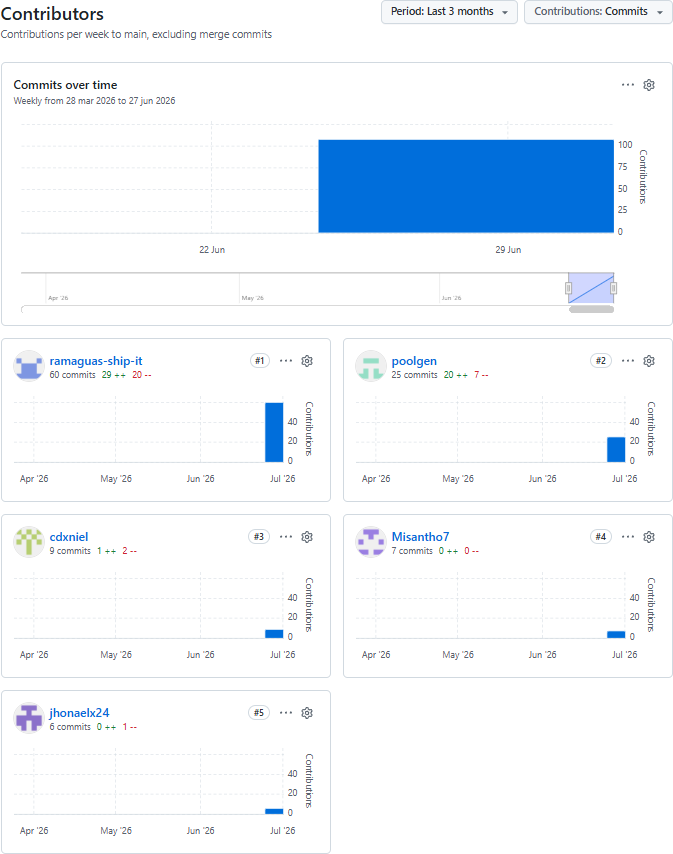
\includegraphics[width=6.16926in,height=7.82833in]{./media/image65.png}
\end{quote}

\protect\phantomsection\label{_bookmark115}{}\emph{\textbf{Ilustración
36. Commits}}

\begin{quote}
Con el fin de evidenciar el trabajo colaborativo del equipo, a
continuación, se presenta el historial de \emph{commits} registrado en
el repositorio de GitHub. Este registro muestra las contribuciones
realizadas por cada integrante durante el desarrollo del proyecto,
permitiendo verificar el seguimiento de cambios y la participación
activa en la elaboración de la documentación y demás entregables.
\end{quote}

\subsection{LISTA DE REQUISITOS CRUDOS
ELICITADOS}\label{lista-de-requisitos-crudos-elicitados}

\begin{quote}
Los siguientes requisitos crudos fueron identificados a partir del
análisis de las dos entrevistas semiestructuradas realizadas y del
análisis del sistema objetivo. Se organizan por área funcional y se
indica la fuente de elicitación para garantizar trazabilidad. La
priorización inicial utiliza el esquema MoSCoW.
\end{quote}

{\def\LTcaptype{none} % do not increment counter
\begin{longtable}[]{@{}
  >{\raggedright\arraybackslash}p{(\linewidth - 8\tabcolsep) * \real{0.0716}}
  >{\raggedright\arraybackslash}p{(\linewidth - 8\tabcolsep) * \real{0.2347}}
  >{\raggedright\arraybackslash}p{(\linewidth - 8\tabcolsep) * \real{0.3814}}
  >{\raggedright\arraybackslash}p{(\linewidth - 8\tabcolsep) * \real{0.1638}}
  >{\raggedright\arraybackslash}p{(\linewidth - 8\tabcolsep) * \real{0.1088}}@{}}
\toprule\noalign{}
\begin{minipage}[b]{\linewidth}\centering
\textbf{ID}
\end{minipage} & \begin{minipage}[b]{\linewidth}\centering
\textbf{Nombre}
\end{minipage} & \begin{minipage}[b]{\linewidth}\centering
\textbf{Descripción}
\end{minipage} & \begin{minipage}[b]{\linewidth}\raggedright
\begin{quote}
\textbf{Fuente (entrevista)}
\end{quote}
\end{minipage} & \begin{minipage}[b]{\linewidth}\centering
\textbf{MoSCoW}
\end{minipage} \\
\midrule\noalign{}
\endhead
\bottomrule\noalign{}
\endlastfoot
\multicolumn{5}{@{}>{\raggedright\arraybackslash}p{(\linewidth - 8\tabcolsep) * \real{0.9603} + 8\tabcolsep}@{}}{%
\textbf{Área 1: Gestión Operativa}} \\
\begin{minipage}[t]{\linewidth}\raggedright
\begin{quote}
\textbf{RC-01}
\end{quote}
\end{minipage} & \begin{minipage}[t]{\linewidth}\raggedright
\begin{quote}
\textbf{Acceso multiplataforma (móvil y escritorio)}
\end{quote}
\end{minipage} & \begin{minipage}[t]{\linewidth}\raggedright
\begin{quote}
El sistema debe ser accesible desde smartphones (Android/iOS) y
computadoras de escritorio, dado que ambos stakeholders indicaron el
teléfono

móvil como dispositivo principal.
\end{quote}
\end{minipage} & \begin{minipage}[t]{\linewidth}\raggedright
\begin{quote}
D3 --- ambas entrevistas
\end{quote}
\end{minipage} & \textbf{Must} \\
\begin{minipage}[t]{\linewidth}\raggedright
\begin{quote}
\textbf{RC-02}
\end{quote}
\end{minipage} & \begin{minipage}[t]{\linewidth}\raggedright
\begin{quote}
\textbf{Centralización de información clínica}
\end{quote}
\end{minipage} & \begin{minipage}[t]{\linewidth}\raggedright
\begin{quote}
El sistema debe centralizar todos los historiales de pacientes (nombre,
edad, raza, peso, diagnósticos, tratamientos) en una única base de datos
consultable.
\end{quote}
\end{minipage} & \begin{minipage}[t]{\linewidth}\raggedright
\begin{quote}
A1/A2 ---

Amagua; A1/A2

--- Dr. Antonio
\end{quote}
\end{minipage} & \textbf{Must} \\
\begin{minipage}[t]{\linewidth}\raggedright
\begin{quote}
\textbf{RC-03}
\end{quote}
\end{minipage} & \begin{minipage}[t]{\linewidth}\raggedright
\begin{quote}
\textbf{Búsqueda rápida por nombre del paciente y nombre del dueño}
\end{quote}
\end{minipage} & \begin{minipage}[t]{\linewidth}\raggedright
\begin{quote}
El sistema debe permitir búsquedas por nombre del animal y por nombre
del propietario para resolver el problema de organización identificado
en Buff Note.
\end{quote}
\end{minipage} & \begin{minipage}[t]{\linewidth}\raggedright
\begin{quote}
A2 --- Amagua ("no está bien organizado el tema de buscar por nombre y

dueño")
\end{quote}
\end{minipage} & \textbf{Must} \\
\begin{minipage}[t]{\linewidth}\raggedright
\begin{quote}
\textbf{RC-04}
\end{quote}
\end{minipage} & \begin{minipage}[t]{\linewidth}\raggedright
\begin{quote}
\textbf{Registro detallado de historial clínico}
\end{quote}
\end{minipage} & \begin{minipage}[t]{\linewidth}\raggedright
\begin{quote}
El sistema debe registrar: nombre, edad, raza, peso, motivo de consulta,
diagnóstico,

tratamiento, dosis, frecuencia de administración y fecha de cada
consulta.
\end{quote}
\end{minipage} & \begin{minipage}[t]{\linewidth}\raggedright
\begin{quote}
A1 --- Amagua; A2 --- Dr.

Antonio
\end{quote}
\end{minipage} & \textbf{Must} \\
\begin{minipage}[t]{\linewidth}\raggedright
\begin{quote}
\textbf{RC-05}
\end{quote}
\end{minipage} & \begin{minipage}[t]{\linewidth}\raggedright
\begin{quote}
\textbf{Control de inventario con alertas de vencimiento automáticas}
\end{quote}
\end{minipage} & \begin{minipage}[t]{\linewidth}\raggedright
\begin{quote}
El sistema debe registrar cada producto con su fecha de vencimiento y
generar alertas automáticas cuando un producto esté a 30, 15 y 7 días de
su fecha de caducidad.
\end{quote}
\end{minipage} & \begin{minipage}[t]{\linewidth}\raggedright
\begin{quote}
A4 --- Dr.

Antonio ("siempre se caducan por falta de precaución"); A4 --- Amagua
("manualmente revisando uno a

uno")
\end{quote}
\end{minipage} & \textbf{Must} \\
\begin{minipage}[t]{\linewidth}\raggedright
\begin{quote}
\textbf{RC-06}
\end{quote}
\end{minipage} & \begin{minipage}[t]{\linewidth}\raggedright
\begin{quote}
\textbf{Gestión de stock con alertas de faltantes}
\end{quote}
\end{minipage} & \begin{minipage}[t]{\linewidth}\raggedright
\begin{quote}
El sistema debe registrar las cantidades en stock y generar alertas
cuando el nivel de

un producto caiga por debajo del umbral mínimo configurado.
\end{quote}
\end{minipage} & \begin{minipage}[t]{\linewidth}\raggedright
\begin{quote}
A4 --- ambas entrevistas
\end{quote}
\end{minipage} & \textbf{Must} \\
\begin{minipage}[t]{\linewidth}\raggedright
\begin{quote}
\textbf{RC-07}
\end{quote}
\end{minipage} & \begin{minipage}[t]{\linewidth}\raggedright
\begin{quote}
\textbf{Registro del proceso de cobro}
\end{quote}
\end{minipage} & \begin{minipage}[t]{\linewidth}\raggedright
\begin{quote}
El sistema debe permitir registrar el cobro de cada consulta, incluyendo
los servicios prestados, productos utilizados y monto cobrado.
\end{quote}
\end{minipage} & \begin{minipage}[t]{\linewidth}\raggedright
\begin{quote}
A3 --- Dr.

Antonio; A3 --- Amagua ("la parte más

demorada")
\end{quote}
\end{minipage} & \textbf{Must} \\
\begin{minipage}[t]{\linewidth}\raggedright
\begin{quote}
\textbf{RC-08}
\end{quote}
\end{minipage} & \begin{minipage}[t]{\linewidth}\raggedright
\begin{quote}
\textbf{Módulo de facturación ágil}
\end{quote}
\end{minipage} & \begin{minipage}[t]{\linewidth}\raggedright
\begin{quote}
El proceso de registro de una factura no debe requerir más de 3 pasos
desde el inicio hasta la emisión, eliminando las demoras identificadas
en el programa

actual.
\end{quote}
\end{minipage} & \begin{minipage}[t]{\linewidth}\raggedright
\begin{quote}
A3 --- Amagua ("es la parte más demorada")
\end{quote}
\end{minipage} & \textbf{Must} \\
\begin{minipage}[t]{\linewidth}\raggedright
\begin{quote}
\textbf{RC-09}
\end{quote}
\end{minipage} & \begin{minipage}[t]{\linewidth}\raggedright
\begin{quote}
\textbf{Registro de comunicaciones post-consulta}
\end{quote}
\end{minipage} & \begin{minipage}[t]{\linewidth}\raggedright
\begin{quote}
El sistema debe registrar las comunicaciones realizadas con los dueños

(tipo: llamada, WhatsApp, mensaje), con fecha y resumen del contenido.
\end{quote}
\end{minipage} & \begin{minipage}[t]{\linewidth}\raggedright
\begin{quote}
A6 --- ambas entrevistas
\end{quote}
\end{minipage} & Should \\
\begin{minipage}[t]{\linewidth}\raggedright
\begin{quote}
\textbf{RC-10}
\end{quote}
\end{minipage} & \begin{minipage}[t]{\linewidth}\raggedright
\begin{quote}
\textbf{Envío de resultados por WhatsApp}
\end{quote}
\end{minipage} & \begin{minipage}[t]{\linewidth}\raggedright
\begin{quote}
El sistema debe permitir adjuntar y enviar resultados de exámenes
directamente por WhatsApp desde la plataforma.
\end{quote}
\end{minipage} & \begin{minipage}[t]{\linewidth}\raggedright
\begin{quote}
A6 --- Amagua ("los resultados de exámenes se
\end{quote}
\end{minipage} & Should \\
\end{longtable}
}

{\def\LTcaptype{none} % do not increment counter
\begin{longtable}[]{@{}
  >{\raggedright\arraybackslash}p{(\linewidth - 8\tabcolsep) * \real{0.0716}}
  >{\raggedright\arraybackslash}p{(\linewidth - 8\tabcolsep) * \real{0.2347}}
  >{\raggedright\arraybackslash}p{(\linewidth - 8\tabcolsep) * \real{0.3814}}
  >{\raggedright\arraybackslash}p{(\linewidth - 8\tabcolsep) * \real{0.1638}}
  >{\centering\arraybackslash}p{(\linewidth - 8\tabcolsep) * \real{0.1088}}@{}}
\toprule\noalign{}
\begin{minipage}[b]{\linewidth}\raggedright
\end{minipage} & \begin{minipage}[b]{\linewidth}\raggedright
\end{minipage} & \begin{minipage}[b]{\linewidth}\raggedright
\end{minipage} & \begin{minipage}[b]{\linewidth}\raggedright
\begin{quote}
lo enviamos

directamente por WhatsApp")
\end{quote}
\end{minipage} & \begin{minipage}[b]{\linewidth}\centering
\end{minipage} \\
\midrule\noalign{}
\endhead
\bottomrule\noalign{}
\endlastfoot
\begin{minipage}[t]{\linewidth}\raggedright
\begin{quote}
\textbf{RC-11}
\end{quote}
\end{minipage} & \begin{minipage}[t]{\linewidth}\raggedright
\begin{quote}
\textbf{Registro de seguimiento de citas e inasistencias}
\end{quote}
\end{minipage} & \begin{minipage}[t]{\linewidth}\raggedright
\begin{quote}
El sistema debe registrar las citas programadas, las asistencias y las
inasistencias, permitiendo conocer la evolución del paciente incluso
cuando no

regresa a control.
\end{quote}
\end{minipage} & \begin{minipage}[t]{\linewidth}\raggedright
\begin{quote}
A5 --- Amagua ("no sabemos qué pasó con el paciente")
\end{quote}
\end{minipage} & \textbf{Must} \\
\begin{minipage}[t]{\linewidth}\raggedright
\begin{quote}
\textbf{RC-12}
\end{quote}
\end{minipage} & \begin{minipage}[t]{\linewidth}\raggedright
\begin{quote}
\textbf{Recordatorios automáticos de citas}
\end{quote}
\end{minipage} & \begin{minipage}[t]{\linewidth}\raggedright
\begin{quote}
El sistema debe enviar recordatorios automáticos (WhatsApp o SMS) al
dueño

de la mascota con 24 horas de antelación a una cita programada.
\end{quote}
\end{minipage} & \begin{minipage}[t]{\linewidth}\raggedright
\begin{quote}
A5 --- Amagua; A6 --- Dr.

Antonio
\end{quote}
\end{minipage} & Should \\
\multicolumn{5}{@{}>{\raggedright\arraybackslash}p{(\linewidth - 8\tabcolsep) * \real{0.9603} + 8\tabcolsep}@{}}{%
\textbf{Área 2: Seguimiento Clínico y Nutricional}} \\
\begin{minipage}[t]{\linewidth}\raggedright
\begin{quote}
\textbf{RC-13}
\end{quote}
\end{minipage} & \begin{minipage}[t]{\linewidth}\raggedright
\begin{quote}
\textbf{Registro de parámetros de crecimiento y peso a lo largo del
tiempo}
\end{quote}
\end{minipage} & \begin{minipage}[t]{\linewidth}\raggedright
\begin{quote}
El sistema debe registrar de forma cronológica el peso, edad y
parámetros de condición corporal del animal en cada visita, permitiendo
visualizar tendencias.
\end{quote}
\end{minipage} & \begin{minipage}[t]{\linewidth}\raggedright
\begin{quote}
B1 --- Dr.

Antonio ("en base a la edad va a agarrar el peso"); B1 ---

Amagua
\end{quote}
\end{minipage} & \textbf{Must} \\
\begin{minipage}[t]{\linewidth}\raggedright
\begin{quote}
\textbf{RC-14}
\end{quote}
\end{minipage} & \begin{minipage}[t]{\linewidth}\raggedright
\begin{quote}
\textbf{Generación de recomendaciones nutricionales personalizadas}
\end{quote}
\end{minipage} & \begin{minipage}[t]{\linewidth}\raggedright
\begin{quote}
El sistema debe generar recomendaciones de alimentación basadas en la
raza, edad, peso y condición de salud del animal, apoyando el juicio del
veterinario.
\end{quote}
\end{minipage} & \begin{minipage}[t]{\linewidth}\raggedright
\begin{quote}
B2 --- Dr.

Antonio ("inculcarle al dueño del perro la alimentación nutritiva
adecuada"); B2

--- Amagua
\end{quote}
\end{minipage} & Should \\
\begin{minipage}[t]{\linewidth}\raggedright
\begin{quote}
\textbf{RC-15}
\end{quote}
\end{minipage} & \begin{minipage}[t]{\linewidth}\raggedright
\begin{quote}
\textbf{Programación de recordatorios de seguimiento de indicaciones
médicas}
\end{quote}
\end{minipage} & \begin{minipage}[t]{\linewidth}\raggedright
\begin{quote}
El sistema debe permitir programar recordatorios para verificar el
cumplimiento de indicaciones (medicación, dieta, reposo) en fechas
establecidas por el

veterinario.
\end{quote}
\end{minipage} & \begin{minipage}[t]{\linewidth}\raggedright
\begin{quote}
B3 --- Amagua ("esperamos que lleguen; si no, no podemos saber")
\end{quote}
\end{minipage} & Should \\
\begin{minipage}[t]{\linewidth}\raggedright
\begin{quote}
\textbf{RC-16}
\end{quote}
\end{minipage} & \begin{minipage}[t]{\linewidth}\raggedright
\begin{quote}
\textbf{Exportación de reportes de salud del paciente}
\end{quote}
\end{minipage} & \begin{minipage}[t]{\linewidth}\raggedright
\begin{quote}
El sistema debe generar y exportar reportes del historial clínico del
paciente en formato PDF para facilitar referencias a clínicas con mayor
equipamiento.
\end{quote}
\end{minipage} & \begin{minipage}[t]{\linewidth}\raggedright
\begin{quote}
B4 --- Dr.

Antonio ("se le indica que hay que hacer pruebas de sangre o llevar a
una clínica con todos los

equipos")
\end{quote}
\end{minipage} & Should \\
\multicolumn{5}{@{}>{\raggedright\arraybackslash}p{(\linewidth - 8\tabcolsep) * \real{0.9603} + 8\tabcolsep}@{}}{%
\textbf{Área 3: Módulo de Inteligencia Artificial}} \\
\begin{minipage}[t]{\linewidth}\raggedright
\begin{quote}
\textbf{RC-17}
\end{quote}
\end{minipage} & \begin{minipage}[t]{\linewidth}\raggedright
\begin{quote}
\textbf{Sugerencias diagnósticas basadas en datos clínicos (con
validación obligatoria)}
\end{quote}
\end{minipage} & \begin{minipage}[t]{\linewidth}\raggedright
\begin{quote}
El sistema debe analizar los datos clínicos ingresados por el
veterinario y sugerir posibles diagnósticos diferenciales.

Ninguna sugerencia puede aplicarse sin revisión y aprobación explícita
del veterinario.
\end{quote}
\end{minipage} & \begin{minipage}[t]{\linewidth}\raggedright
\begin{quote}
C2/C4 ---

Amagua ("si tengo que dar un visto bueno antes, sí"); C4

--- Dr. Antonio ("confianza moderada")
\end{quote}
\end{minipage} & \textbf{Must} \\
\begin{minipage}[t]{\linewidth}\raggedright
\begin{quote}
\textbf{RC-18}
\end{quote}
\end{minipage} & \begin{minipage}[t]{\linewidth}\raggedright
\begin{quote}
\textbf{Respaldo de recomendaciones en literatura científica veterinaria
validada}
\end{quote}
\end{minipage} & \begin{minipage}[t]{\linewidth}\raggedright
\begin{quote}
Cada sugerencia del módulo de IA debe indicar su fuente bibliográfica
científica para que el veterinario pueda evaluarla.
\end{quote}
\end{minipage} & \begin{minipage}[t]{\linewidth}\raggedright
\begin{quote}
C5 --- ambas entrevistas (primera opción seleccionada en

ambos casos)
\end{quote}
\end{minipage} & \textbf{Must} \\
\begin{minipage}[t]{\linewidth}\raggedright
\begin{quote}
\textbf{RC-19}
\end{quote}
\end{minipage} & \begin{minipage}[t]{\linewidth}\raggedright
\begin{quote}
\textbf{Capacidad de revisión y corrección de sugerencias de IA por
parte del veterinario}
\end{quote}
\end{minipage} & \begin{minipage}[t]{\linewidth}\raggedright
\begin{quote}
El sistema debe permitir al veterinario ver, modificar o rechazar
cualquier sugerencia del módulo de IA antes de registrarla en el
historial del paciente.
\end{quote}
\end{minipage} & \begin{minipage}[t]{\linewidth}\raggedright
\begin{quote}
C5 --- Amagua (segunda opción); C5 --- Dr. Antonio
\end{quote}
\end{minipage} & \textbf{Must} \\
\multicolumn{5}{@{}>{\raggedright\arraybackslash}p{(\linewidth - 8\tabcolsep) * \real{0.9603} + 8\tabcolsep}@{}}{%
\textbf{Área 4: Usabilidad, Acceso y Calidad del Sistema}} \\
\end{longtable}
}

{\def\LTcaptype{none} % do not increment counter
\begin{longtable}[]{@{}
  >{\raggedright\arraybackslash}p{(\linewidth - 8\tabcolsep) * \real{0.0716}}
  >{\raggedright\arraybackslash}p{(\linewidth - 8\tabcolsep) * \real{0.2347}}
  >{\raggedright\arraybackslash}p{(\linewidth - 8\tabcolsep) * \real{0.3814}}
  >{\raggedright\arraybackslash}p{(\linewidth - 8\tabcolsep) * \real{0.1638}}
  >{\centering\arraybackslash}p{(\linewidth - 8\tabcolsep) * \real{0.1088}}@{}}
\toprule\noalign{}
\begin{minipage}[b]{\linewidth}\raggedright
\begin{quote}
\textbf{RC-20}
\end{quote}
\end{minipage} & \begin{minipage}[b]{\linewidth}\raggedright
\begin{quote}
\textbf{Interfaz sencilla sin capacitación prolongada}
\end{quote}
\end{minipage} & \begin{minipage}[b]{\linewidth}\raggedright
\begin{quote}
El sistema debe poder ser utilizado por un veterinario con experiencia
digital básica sin necesidad de un proceso de formación mayor a 2 horas.
\end{quote}
\end{minipage} & \begin{minipage}[b]{\linewidth}\raggedright
\begin{quote}
D2 --- Dr.

Antonio ("que sea fácil de usar"); D2 --- Amagua ("facilidad de

utilizarla")
\end{quote}
\end{minipage} & \begin{minipage}[b]{\linewidth}\centering
\textbf{Must}
\end{minipage} \\
\midrule\noalign{}
\endhead
\bottomrule\noalign{}
\endlastfoot
\begin{minipage}[t]{\linewidth}\raggedright
\begin{quote}
\textbf{RC-21}
\end{quote}
\end{minipage} & \begin{minipage}[t]{\linewidth}\raggedright
\begin{quote}
\textbf{Operación con baja dependencia de conectividad permanente}
\end{quote}
\end{minipage} & \begin{minipage}[t]{\linewidth}\raggedright
\begin{quote}
El sistema debe permitir el registro y consulta de historiales clínicos
de manera local cuando no haya conexión a internet, sincronizando
automáticamente al restablecerse la conexión.
\end{quote}
\end{minipage} & \begin{minipage}[t]{\linewidth}\raggedright
\begin{quote}
D4 --- Dr.

Antonio (nivel 2-3/5 de cortes); D4 --- Amagua (rara vez, pero

ocurre)
\end{quote}
\end{minipage} & Should \\
\begin{minipage}[t]{\linewidth}\raggedright
\begin{quote}
\textbf{RC-22}
\end{quote}
\end{minipage} & \begin{minipage}[t]{\linewidth}\raggedright
\begin{quote}
\textbf{Bajo costo de implementación y operación}
\end{quote}
\end{minipage} & \begin{minipage}[t]{\linewidth}\raggedright
\begin{quote}
El sistema debe contemplar un modelo de costos accesible para clínicas
de 1 a 3 veterinarios, siendo este un criterio

explícito de adopción.
\end{quote}
\end{minipage} & \begin{minipage}[t]{\linewidth}\raggedright
\begin{quote}
D2 --- Dr.

Antonio ("bajo valor

económico")
\end{quote}
\end{minipage} & \textbf{Must} \\
\begin{minipage}[t]{\linewidth}\raggedright
\begin{quote}
\textbf{RC-23}
\end{quote}
\end{minipage} & \begin{minipage}[t]{\linewidth}\raggedright
\begin{quote}
\textbf{Perfiles de usuario diferenciados con control de acceso}
\end{quote}
\end{minipage} & \begin{minipage}[t]{\linewidth}\raggedright
\begin{quote}
El sistema debe gestionar al menos dos tipos de perfil de usuario:
médico veterinario y personal administrativo, con accesos y permisos
diferenciados por rol.
\end{quote}
\end{minipage} & \begin{minipage}[t]{\linewidth}\raggedright
\begin{quote}
Sección C/D --- ambas entrevistas; RC identificado por

el equipo
\end{quote}
\end{minipage} & \textbf{Must} \\
\begin{minipage}[t]{\linewidth}\raggedright
\begin{quote}
\textbf{RC-24}
\end{quote}
\end{minipage} & \begin{minipage}[t]{\linewidth}\raggedright
\begin{quote}
\textbf{Trazabilidad de cambios en historiales clínicos}
\end{quote}
\end{minipage} & \begin{minipage}[t]{\linewidth}\raggedright
\begin{quote}
El sistema debe registrar automáticamente quién realizó cada
modificación en un historial clínico, con fecha y descripción

del cambio.
\end{quote}
\end{minipage} & \begin{minipage}[t]{\linewidth}\raggedright
\begin{quote}
Derivado de RC-04 y RC-17 ---

buenas prácticas de IA clínica
\end{quote}
\end{minipage} & Should \\
\end{longtable}
}

\protect\phantomsection\label{_bookmark117}{}\emph{\textbf{Tabla 30.
Requisitos crudos elicitados}}

\paragraph{\texorpdfstring{ \ul{Notas de Ajuste respecto al Documento
Proyecto\_1\_vcty}
}{ Notas de Ajuste respecto al Documento Proyecto\_1\_vcty }}\label{notas-de-ajuste-respecto-al-documento-proyecto_1_vcty}

\begin{quote}
En comparación con la lista de requisitos del documento original
(Proyecto\_1\_vcty), se realizaron los siguientes ajustes basados en las
entrevistas reales:
\end{quote}

\begin{itemize}
\item
  RC-03 (NUEVO): Se agregó búsqueda por nombre del dueño además del
  nombre del animal, problema específico identificado por Amagua con
  Buff Note.
\item
  RC-07 y RC-08 (AMPLIADOS): Se separó el registro de cobro (RC-07) de
  la facturación ágil (RC-08), y se añadió el criterio de no más de 3
  pasos basado en el dolor específico de Amagua.
\item
  RC-10 (NUEVO): Envío de resultados por WhatsApp, uso confirmado
  directamente por Amagua.
\item
  RC-17/RC-18/RC-19 (REFINADOS): Los requisitos de IA se desagregaron en
  tres requisitos separados para mayor trazabilidad; la condición de
  validación obligatoria del veterinario es un Must, no un Should.
\item
  RC-21 (AJUSTADO): La operación offline se mantiene como Should (no
  Must) porque Amagua reportó baja frecuencia de cortes (nivel 1-2/5).
\item
  RC-22 (NUEVO): El bajo costo fue mencionado explícitamente como
  criterio de adopción por Dr. Antonio; se eleva a Must.
\item
  RC original "módulo de configuración para bajo costo" se elimina como
  requisito técnico y se convierte en RC-22 de criterio de negocio.
\end{itemize}

\subsection{REFERENCIAS}\label{referencias-1}

\begin{enumerate}
\def\labelenumi{\arabic{enumi}.}
\item
  I. Sommerville, Ingeniería de Software, 10.a ed. Madrid, España:
  Pearson, 2016.
\item
  E. H. Shortliffe y J. J. Cimino, Eds., Biomedical Informatics:
  Computer Applications in Health Care and Biomedicine. New York, NY,
  USA: Springer, 2014.
\item
  E. J. Topol, Deep Medicine: How Artificial Intelligence Can Make
  Healthcare Human Again. New York, NY, USA: Basic Books, 2019.
\item
  R. Haux, A. Winter, E. Ammenwerth y B. Brigl, Strategic Information
  Management in Hospitals: An Introduction to Hospital Information
  Systems. Cham, Switzerland: Springer Nature, 2018.
\item
  IEEE/ISO/IEC 29148:2018, Systems and Software Engineering --- Life
  Cycle Processes --- Requirements Engineering. Geneva, Switzerland:
  ISO/IEC, 2018.
\item
  ISO/IEC 25010:2023, Systems and Software Quality Requirements and
  Evaluation (SQuaRE). Geneva, Switzerland: ISO/IEC, 2023.
\item
  H. Washizaki (Ed.), SWEBOK Guide v4.0. IEEE Computer Society, 2024.
\item
  K. Pohl, Requirements Engineering: Fundamentals, Principles, and
  Techniques. Heidelberg, Germany: Springer, 2010.
\end{enumerate}

\end{document}
